\documentclass{../course_template/lectureClass}


\title[Control of three-phase drives]{Control of three-phase drives}
\author{Oliver Wallscheid}
\date{}

\makeglossaries
% Course-related individual configuration deviating from the general course template settings 

\hypersetup{bookmarksdepth=4} % Set depth of PDF bookmarks to include sections, subsections, and subsubsections


% Reconfiguration of TOC (Table of Contents) to include subsubsections
\AtBeginSection[]
{
    \hypertarget{sec\thesection}{}
    \begin{frame}{Table of contents}
        \tableofcontents[sectionstyle=show/hide,subsectionstyle=show/show/hide,
            subsubsectionstyle=hide/hide/hide/hide]
    \end{frame}
}

\AtBeginSubsection[]
{
    \ifnum\value{subsection} > 1 % show TOC again after the second subsection
        \begin{frame}{Table of contents}
            \tableofcontents[sectionstyle=show/hide,subsectionstyle=show/shaded/hide,
                subsubsectionstyle=show/show/hide/hide]
        \end{frame}
    \fi
}

\AtBeginSubsubsection[]
{

    \ifnum\value{subsubsection} > 1 % show TOC again after the second subsection
        \begin{frame}{Table of contents}
            \tableofcontents[sectionstyle=show/hide,subsectionstyle=show/shaded/hide,
                subsubsectionstyle=show/shaded/hide/hide]
        \end{frame}
    \fi
}


% Helper functions and parameters for OPS plots / normalize IPMSM
%-------------------------------------------------------------------------
% Simplified linear IPMSM model for visualizing the operating regions:
%   psi_d = psi_PM + L_d i_{s,d},
%   psi_q = L_q i_{s,q},
%   T = K_T (psi_PM - (L_q-L_d)i_{s,d}) i_{s,q}.
%
% Normalization:
%   x = i_{s,d}/I_max, y = i_{s,q}/I_max.
% Thus, the current constraint becomes x^2 + y^2 = 1.
%
% Voltage model for the loci, with R_s neglected for clarity:
%   (psi_PM + L_d I_max x)^2 + (L_q I_max y)^2 = c^2,
%   c = u_{s,max}/omega.
%
% Color convention used below:
%   signaldelta   -> current constraint
%   signalalpha   -> voltage constraint
%   signalbeta    -> MTPC contour
%   signalepsilon -> MTPV contour
% -------------------------------------------------------------------------

\pgfmathsetmacro{\psim}{1.1}
\pgfmathsetmacro{\Ld}{0.4}
\pgfmathsetmacro{\Lq}{0.8}
\pgfmathsetmacro{\DeltaL}{\Lq-\Ld}
\pgfmathsetmacro{\Kt}{1.0}
\pgfmathsetmacro{\Imax}{5.0}

% Analytic functions in physical coordinates.
\pgfmathdeclarefunction{torque}{2}{%
    \pgfmathparse{\Kt*(\psim-\DeltaL*(#1))*(#2)}%
}
\pgfmathdeclarefunction{idmtpc}{1}{%
    \pgfmathparse{\psim/(2*\DeltaL)-sqrt((\psim/(2*\DeltaL))^2 + (#1)^2)}%
}
\pgfmathdeclarefunction{iqvoltage}{2}{%
    \pgfmathparse{sqrt(max(0,(#2)*(#2)-(\psim+\Ld*(#1))*(\psim+\Ld*(#1))))/\Lq}%
}
\pgfmathdeclarefunction{iqtorque}{2}{%
    \pgfmathparse{(#2)/(\Kt*(\psim-\DeltaL*(#1)))}%
}
\pgfmathdeclarefunction{iqmtpv}{1}{%
    \pgfmathparse{sqrt(max(0,-\Ld*(\psim+\Ld*(#1))*(\psim-\DeltaL*(#1))/(\DeltaL*\Lq*\Lq)))}%
}

% Analytic functions in normalized coordinates.
\pgfmathdeclarefunction{xmtpcnorm}{1}{%
    \pgfmathparse{idmtpc(\Imax*abs(#1))/\Imax}%
}
\pgfmathdeclarefunction{ycurrentnorm}{1}{%
    \pgfmathparse{sqrt(max(0,1-(#1)*(#1)))}%
}
\pgfmathdeclarefunction{xcurrentnorm}{1}{%
    \pgfmathparse{-sqrt(max(0,1-(#1)*(#1)))}%
}
\pgfmathdeclarefunction{yvoltnorm}{2}{%
    \pgfmathparse{iqvoltage(\Imax*(#1),#2)/\Imax}%
}
\pgfmathdeclarefunction{ytorquenorm}{2}{%
    \pgfmathparse{iqtorque(\Imax*(#1),#2)/\Imax}%
}
\pgfmathdeclarefunction{ymtpvnorm}{1}{%
    \pgfmathparse{iqmtpv(\Imax*(#1))/\Imax}%
}

% Inverse MTPV relation x = x_MTPV(y), derived from the quadratic equation
% of the analytic MTPV locus. The negative root gives the relevant branch.
\pgfmathdeclarefunction{xmtpvnorm}{1}{%
    \pgfmathparse{%
        -(-\Ld*\psim*(\Ld*\Imax-\DeltaL*\Imax))/(2*\Ld*(\Ld*\Imax)*(\DeltaL*\Imax))
        -
        sqrt((-\Ld*\psim*(\Ld*\Imax-\DeltaL*\Imax))^2
        -4*(\Ld*(\Ld*\Imax)*(\DeltaL*\Imax))
        *(-\Ld*\psim*\psim-\DeltaL*\Lq*\Lq*\Imax*\Imax*(#1)*(#1)))
        /(2*\Ld*(\Ld*\Imax)*(\DeltaL*\Imax))%
    }%
}


% Helper functions and parameters for IM OPS plots
% -------------------------------------------------------------------------
% Normalized rotor-flux-oriented IM example:
%   x = i_{s,d}^{psi_r}/i_{s,max}, y = i_{s,q}^{psi_r}/i_{s,max}
%   L_m(x) follows a mild apparent main-inductance saturation law,
%   while L_{sigma s} and L_{sigma r} are constant.
% All trajectories below are evaluated online by pgfmath/PGFPlots.
% -------------------------------------------------------------------------


\pgfmathsetmacro{\imLmZero}{1.0}
\pgfmathsetmacro{\imSatA}{0.20}
\pgfmathsetmacro{\imSatB}{0.70}
\pgfmathsetmacro{\imLsigmas}{0.15}
\pgfmathsetmacro{\imLsigmar}{0.12}
\pgfmathsetmacro{\imRs}{1.00}
\pgfmathsetmacro{\imRr}{0.80}

\pgfmathdeclarefunction{imLm}{1}{%
    \pgfmathparse{\imLmZero*(1-\imSatA*(#1)*(#1)/(1+\imSatB*(#1)*(#1)))}%
}
\pgfmathdeclarefunction{imLmPrime}{1}{%
    \pgfmathparse{\imLmZero*(-2*\imSatA*abs(#1))/((1+\imSatB*(#1)*(#1))*(1+\imSatB*(#1)*(#1)))}%
}
\pgfmathdeclarefunction{imLs}{1}{%
    \pgfmathparse{\imLsigmas+imLm(abs(#1))}%
}
\pgfmathdeclarefunction{imLr}{1}{%
    \pgfmathparse{\imLsigmar+imLm(abs(#1))}%
}
\pgfmathdeclarefunction{imBeta}{1}{%
    \pgfmathparse{imLm(abs(#1))/imLr(abs(#1))}%
}
\pgfmathdeclarefunction{imBetaPrime}{1}{%
    \pgfmathparse{imLmPrime(abs(#1))*\imLsigmar/(imLr(abs(#1))*imLr(abs(#1)))}%
}
\pgfmathdeclarefunction{imEta}{1}{%
    \pgfmathparse{imLm(abs(#1))*imLm(abs(#1))/imLr(abs(#1))}%
}
\pgfmathdeclarefunction{imEtaPrime}{1}{%
    \pgfmathparse{imLmPrime(abs(#1))*imLm(abs(#1))*(2*imLr(abs(#1))-imLm(abs(#1)))/(imLr(abs(#1))*imLr(abs(#1)))}%
}
\pgfmathdeclarefunction{imA}{1}{%
    \pgfmathparse{imEta(abs(#1))*abs(#1)}%
}
\pgfmathdeclarefunction{imAprime}{1}{%
    \pgfmathparse{imEta(abs(#1))+abs(#1)*imEtaPrime(abs(#1))}%
}
\pgfmathdeclarefunction{imBcu}{1}{%
    \pgfmathparse{\imRs+\imRr*imBeta(abs(#1))*imBeta(abs(#1))}%
}
\pgfmathdeclarefunction{imBcuPrime}{1}{%
    \pgfmathparse{2*\imRr*imBeta(abs(#1))*imBetaPrime(abs(#1))}%
}
\pgfmathdeclarefunction{imSigmaEff}{1}{%
    \pgfmathparse{imLs(abs(#1))-imEta(abs(#1))}%
}
\pgfmathdeclarefunction{imSigmaEffPrime}{1}{%
    \pgfmathparse{imLmPrime(abs(#1))-imEtaPrime(abs(#1))}%
}
\pgfmathdeclarefunction{imFluxD}{1}{%
    \pgfmathparse{imLs(abs(#1))*abs(#1)}%
}
\pgfmathdeclarefunction{imFluxDsq}{1}{%
    \pgfmathparse{imFluxD(abs(#1))*imFluxD(abs(#1))}%
}
\pgfmathdeclarefunction{imFluxDsqPrime}{1}{%
    \pgfmathparse{2*imLs(abs(#1))*abs(#1)*(imLs(abs(#1))+abs(#1)*imLmPrime(abs(#1)))}%
}
\pgfmathdeclarefunction{imFluxQweight}{1}{%
    \pgfmathparse{imSigmaEff(abs(#1))*imSigmaEff(abs(#1))}%
}
\pgfmathdeclarefunction{imFluxQweightPrime}{1}{%
    \pgfmathparse{2*imSigmaEff(abs(#1))*imSigmaEffPrime(abs(#1))}%
}
\pgfmathdeclarefunction{imTorqueRaw}{2}{%
    \pgfmathparse{imA(abs(#1))*(#2)}%
}
\pgfmathdeclarefunction{imPsirRaw}{1}{%
    \pgfmathparse{imLm(abs(#1))*abs(#1)}%
}
\pgfmathdeclarefunction{imPsisRaw}{2}{%
    \pgfmathparse{sqrt(imFluxD(abs(#1))*imFluxD(abs(#1)) + imSigmaEff(abs(#1))*imSigmaEff(abs(#1))*(#2)*(#2))}%
}
\pgfmathdeclarefunction{imCurrentY}{1}{%
    \pgfmathparse{sqrt(max(0,1-(#1)*(#1)))}%
}
\pgfmathdeclarefunction{imTorqueY}{2}{%
    \pgfmathparse{(#2)/max(0.0001,imA(abs(#1)))}%
}
\pgfmathdeclarefunction{imMTPCY}{1}{%
    \pgfmathparse{sqrt(max(0,(abs(#1)*imA(abs(#1)))/max(0.0001,imAprime(abs(#1)))))}%
}
\pgfmathdeclarefunction{imMTPLY}{1}{%
    \pgfmathparse{sqrt(max(0,(2*\imRs*abs(#1))/max(0.0001,2*imBcu(abs(#1))*imAprime(abs(#1))/max(0.0001,imA(abs(#1)))-imBcuPrime(abs(#1)))))}%
}
\pgfmathdeclarefunction{imMTPFY}{1}{%
    \pgfmathparse{sqrt(max(0,imFluxDsqPrime(abs(#1))/max(0.0001,2*imFluxQweight(abs(#1))*imAprime(abs(#1))/max(0.0001,imA(abs(#1)))-imFluxQweightPrime(abs(#1)))))}%
}
\pgfmathdeclarefunction{imPcuRaw}{2}{%
    \pgfmathparse{\imRs*((#1)*(#1)+(#2)*(#2))+\imRr*imBeta(abs(#1))*imBeta(abs(#1))*(#2)*(#2)}%
}

% Current-circle intersections of the three online-calculated trajectories.
% The displayed curves remain PGFPlots function plots; these constants only
% define the visible end points of the feasible branches for the chosen example.
\pgfmathsetmacro{\imxRMTPC}{0.683}
\pgfmathsetmacro{\imyRMTPC}{imMTPCY(\imxRMTPC)}
\pgfmathsetmacro{\imxRMTPL}{0.764}
\pgfmathsetmacro{\imyRMTPL}{imMTPLY(\imxRMTPL)}
\pgfmathsetmacro{\imxRMTPF}{0.219}
\pgfmathsetmacro{\imyRMTPF}{imMTPFY(\imxRMTPF)}

\pgfmathsetmacro{\imTN}{imTorqueRaw(\imxRMTPC,\imyRMTPC)}
\pgfmathsetmacro{\imPsiRMax}{imPsirRaw(1)}
\pgfmathsetmacro{\imPsiRN}{imPsirRaw(\imxRMTPC)}
\pgfmathsetmacro{\imPsiSMax}{imPsisRaw(\imxRMTPC,\imyRMTPC)}

\pgfmathdeclarefunction{imTorqueNorm}{2}{%
    \pgfmathparse{imTorqueRaw(#1,#2)/\imTN}%
}
\pgfmathdeclarefunction{imPsiRNorm}{1}{%
    \pgfmathparse{imPsirRaw(#1)/\imPsiRMax}%
}
\pgfmathdeclarefunction{imPsiRNNorm}{1}{%
    \pgfmathparse{imPsirRaw(#1)/\imPsiRN}%
}
\pgfmathdeclarefunction{imPsiSNorm}{2}{%
    \pgfmathparse{imPsisRaw(#1,#2)/\imPsiSMax}%
}

\pgfmathsetmacro{\imPcuN}{imPcuRaw(\imxRMTPC,\imyRMTPC)}
\pgfmathdeclarefunction{imPcuNorm}{2}{%
    \pgfmathparse{imPcuRaw(#1,#2)/\imPcuN}%
}
\pgfmathdeclarefunction{imPcuY}{2}{%
    \pgfmathparse{sqrt(max(0,((#2)-\imRs*(#1)*(#1))/max(0.0001,imBcu(abs(#1)))))}%
}
\pgfmathdeclarefunction{imPsiSY}{2}{%
    \pgfmathparse{sqrt(max(0,((#2)*(#2)-imFluxD(abs(#1))*imFluxD(abs(#1)))/max(0.0001,imFluxQweight(abs(#1)))))}%
}
\pgfmathdeclarefunction{imOmegaNorm}{2}{%
    \pgfmathparse{\imPsiSMax/max(0.0001,imPsisRaw(#1,#2))}%
}

\pgfmathsetmacro{\imxExMTPC}{0.48}
\pgfmathsetmacro{\imyExMTPC}{imMTPCY(\imxExMTPC)}
\pgfmathsetmacro{\imTExMTPC}{imTorqueRaw(\imxExMTPC,\imyExMTPC)}
\pgfmathsetmacro{\imIExMTPC}{sqrt(\imxExMTPC*\imxExMTPC+\imyExMTPC*\imyExMTPC)}
\pgfmathsetmacro{\imPsiVMTPC}{0.75}
\pgfmathsetmacro{\imxPsiVMTPC}{0.72}

\pgfmathsetmacro{\imxExMTPL}{0.47}
\pgfmathsetmacro{\imyExMTPL}{imMTPLY(\imxExMTPL)}
\pgfmathsetmacro{\imTExMTPL}{imTorqueRaw(\imxExMTPL,\imyExMTPL)}
\pgfmathsetmacro{\imPcuExMTPL}{0.45}
\pgfmathsetmacro{\imxPcuExMTPL}{0.671}
\pgfmathsetmacro{\imPsiVMTPL}{0.75}
\pgfmathsetmacro{\imxPsiVMTPL}{0.696}

\pgfmathsetmacro{\imxExFW}{0.34}
\pgfmathsetmacro{\imPsiExFW}{0.44}
\pgfmathsetmacro{\imyExFW}{imPsiSY(\imxExFW,\imPsiExFW)}
\pgfmathsetmacro{\imTExFW}{imTorqueRaw(\imxExFW,\imyExFW)}
\pgfmathsetmacro{\imxPsiExFW}{0.395}

\pgfmathsetmacro{\imxExMC}{0.50}
\pgfmathsetmacro{\imyExMC}{imCurrentY(\imxExMC)}
\pgfmathsetmacro{\imTExMC}{imTorqueRaw(\imxExMC,\imyExMC)}
\pgfmathsetmacro{\imPsiExMC}{0.78}
\pgfmathsetmacro{\imxPsiExMC}{0.732}

\pgfmathsetmacro{\imxExMTPF}{0.17}
\pgfmathsetmacro{\imyExMTPF}{imMTPFY(\imxExMTPF)}
\pgfmathsetmacro{\imTExMTPF}{imTorqueRaw(\imxExMTPF,\imyExMTPF)}
\pgfmathsetmacro{\imPsiExMTPF}{imPsisRaw(\imxExMTPF,\imyExMTPF)}
\pgfmathsetmacro{\imxPsiExMTPF}{0.25}

\pgfmathsetmacro{\imxTSend}{0.1565}
\pgfmathsetmacro{\imOmegaMaxPlot}{3.00}

\pgfmathsetmacro{\imOmegaMTPLedge}{imOmegaNorm(\imxRMTPL,\imyRMTPL)}
\pgfmathsetmacro{\imTorqueMTPLedge}{imTorqueNorm(\imxRMTPL,\imyRMTPL)}
\pgfmathsetmacro{\imOmegaMTPFedge}{imOmegaNorm(\imxRMTPF,\imyRMTPF)}

\pgfplotsset{
    imsataxis/.style={
            width=6.5cm,
            height=4.8cm,
            xmin=0, xmax=1.05,
            ymin=0.82, ymax=1.02,
            axis lines=left,
            xlabel={$i_{\mathrm{s,d}}^{\psi_{\mathrm r}}/i_{\mathrm{s,max}}$},
            ylabel={$L_{\mathrm{m}}/L_{\mathrm{m},0}$},
            grid=major,
            tick label style={font=\small},
            label style={font=\small}
        },
    imcurrentaxis/.style={
            width=10.5cm,
            height=7.5cm,
            xmin=0.0, xmax=1.05,
            ymin=0.0, ymax=1.10,
            axis lines=left,
            axis equal image,
            xlabel={$i_{\mathrm{s,d}}/i_{\mathrm{s,max}}$},
            ylabel={$i_{\mathrm{s,q}}/i_{\mathrm{s,max}}$},
            grid=major,
            tick label style={font=\small},
            label style={font=\small},
            clip=true,
            unbounded coords=discard,
            filter discard warning=false
        },
    immapaxis/.style={
            width=7.2cm,
            height=5.6cm,
            xmin=0.0, xmax=1.05,
            ymin=0.0, ymax=1.08,
            axis lines=left,
            xlabel={$T^*/T_{\max}$},
            ylabel={$\psi^*_{\mathrm r}/\psi_{\mathrm{r,N}}$},
            grid=major,
            tick label style={font=\small},
            label style={font=\small},
            legend style={draw=black,fill=white,font=\scriptsize,legend cell align=left},
            clip=false
        },
    imtmaxaxis/.style={
            width=7.2cm,
            height=5.6cm,
            xmin=0.0, xmax=1.08,
            ymin=0.0, ymax=1.10,
            axis lines=left,
            xlabel={$\psi^*_{\mathrm r}/\psi_{\mathrm{r,N}}$},
            ylabel={$T^*_{\lim}/T_{\max}$},
            grid=major,
            tick label style={font=\small},
            label style={font=\small},
            legend style={draw=black,fill=white,font=\scriptsize,legend cell align=left},
            clip=false
        },
    imspeedaxis/.style={
            width=13.4cm,
            height=7.15cm,
            xmin=0, xmax=3.0,
            ymin=0, ymax=1.10,
            axis lines=left,
            axis line style={-Latex},
            xlabel={$\omega/\omega_{\mathrm{nom}}$},
            ylabel={$T^*/T_{\mathrm{max}}$},
            grid=major,
            major grid style={gray!35},
            xtick={0,0.2,...,3.0},
            ytick={0,0.2,...,1.0},
            tick label style={font=\small},
            label style={font=\small},
            clip=false,
            legend style={draw=none,fill=none,font=\small},
        }
}

 % Course-specific configuration (deviating from general course template settings)

\includeonly{tex/Lecture04} % build only selected section


\begin{document}

%%%%%%%%%%%%%%%%%%%%%%%%%%%%%%%%%%%%%%%%%%%%%%%%%%%%%%%%%%%%%
%% Cover slide %%
%%%%%%%%%%%%%%%%%%%%%%%%%%%%%%%%%%%%%%%%%%%%%%%%%%%%%%%%%%%%%

\begin{frame}[plain]
    \titlepage
\end{frame}

%%%%%%%%%%%%%%%%%%%%%%%%%%%%%%%%%%%%%%%%%%%%%%%%%%%%%%%%%%%%%
%% Outline / table of content %%
%%%%%%%%%%%%%%%%%%%%%%%%%%%%%%%%%%%%%%%%%%%%%%%%%%%%%%%%%%%%%
\begin{frame}{Table of contents}
    \tableofcontents[hideallsubsections]
\end{frame}

%%%%%%%%%%%%%%%%%%%%%%%%%%%%%%%%%%%%%%%%%%%%%%%%%%%%%%%%%%%%%
%% Lecture sections %%
%%%%%%%%%%%%%%%%%%%%%%%%%%%%%%%%%%%%%%%%%%%%%%%%%%%%%%%%%%%%%

\include{tex/Lecture01} % Initial overview

%%%%%%%%%%%%%%%%%%%%%%%%%%%%%%%%%%%%%%%%%%%%%%%%%%%%%%%%%%%%%%%%%%
\section{Inverter hardware and modulation techniques}
%%%%%%%%%%%%%%%%%%%%%%%%%%%%%%%%%%%%%%%%%%%%%%%%%%%%%%%%%%%%%%%%%%

%%%%%%%%%%%%%%%%%%%%%%%%%%%%%%%%%%%%%%%%%%%%%%%%%%%%%%%%%%%%%%%%%%
\subsection{Two-level voltage source inverter}
%%%%%%%%%%%%%%%%%%%%%%%%%%%%%%%%%%%%%%%%%%%%%%%%%%%%%%%%%%%%%%%%%%

%%%%%%%%%%%%%%%%%%%%%%%%%%%%%%%%%%%%%%%%%%%%%%%%%%%%%%%%%%%%%
%% Two-level voltage source inverter (2L-VSI) %%
%%%%%%%%%%%%%%%%%%%%%%%%%%%%%%%%%%%%%%%%%%%%%%%%%%%%%%%%%%%%%
\begin{frame}
    \frametitle{Two-level voltage source inverter (2L-VSI)}
    \begin{figure}
        \begin{circuitikz}
            \draw (0,0) node[cute spdt up arrow, xscale=-1] (Sw1) {};
            \draw (1.5,-1.5) node[cute spdt down arrow, xscale=-1] (Sw2) {};
            \draw (3,-3) node[cute spdt down arrow, xscale=-1] (Sw3) {};
            \draw (Sw2.in) to [short, -o] ++(4,0) coordinate (out2);
            \draw (Sw1.in) to [short] ++(3.75,0) to [short, -o] (Sw1.in -| out2) coordinate (out1);
            \draw (Sw3.in) to [short, i=$i_{\mathrm{c}}(t)$] ($(Sw3.in |- Sw3.in)!0.5!(Sw3.in -| out2)$) to [short, -o] (Sw3.in -| out2) coordinate (out3);
            \draw (Sw3.in |- Sw2.in) to [short, i=$i_{\mathrm{b}}(t)$] ($(Sw3.in |- Sw2.in)!0.5!(Sw2.in -| out2)$) to [short, -o] (Sw2.in -| out2);
            \draw (Sw3.in |- Sw1.in) to [short, i=$i_{\mathrm{a}}(t)$] ($(Sw3.in |- Sw1.in)!0.5!(Sw1.in -| out2)$) to [short, -o] (Sw1.in -| out2);
            \draw (out1) to [open, v^=$u_{\mathrm{a\text{-}b}}(t)$, voltage = straight] (out2);
            \draw (out2) to [open, v^=$u_{\mathrm{b\text{-}c}}(t)$, voltage = straight] (out3);
            \draw ($(out3) + (1.5,0)$) to [open, v_=$u_{\mathrm{c\text{-}a}}(t)$, voltage = straight] ($(out1) + (1.5,0)$);
            \draw (Sw1-out 1.n) to [short, -*] ++(0,0.5) coordinate (int1);
            \draw (Sw3-out 2.s) to [short] ++(0,-0.5) coordinate (int3);
            \draw (int3) to [short] (int3 -| Sw1-out 2.s) coordinate (int4) to [short, *-] (Sw1-out 2.s);
            \draw node[crossingshape, name=x1, rotate=-90] at (out1 -| Sw2-out 1.n) {};
            \draw (x1.west) to [short] (int1 -| x1.west) coordinate (int2) to [short] (int1);
            \draw (x1.east) to [short] (Sw2-out 1.n);
            \draw (int1) to [short] ++(-1,0) to [short, i_<=$i_\mathrm{dc}(t)$, -o] ++(-1,0) coordinate (in1);
            \draw (int4) to [short, -o] ++(-2,0) coordinate (in2);
            \draw (in1) to [open, v=$\frac{u_\mathrm{dc}(t)}{2}$, voltage = straight] ($(in2)!0.5!(in1)$) coordinate (mid);
            \draw (mid) to [open, v=$\frac{u_\mathrm{dc}(t)}{2}$, voltage = straight] (in2);
            \draw (mid) node[rground, rotate=-90, name = gnd1]{};
            \draw node[anchor = east, xshift=-0.3cm] at (Sw1) {$s_1(t)$};
            \draw node[anchor = east, xshift=-0.3cm] at (Sw2) {$s_2(t)$};
            \draw node[anchor = east, xshift=-0.3cm] at (Sw3) {$s_3(t)$};
            \draw (Sw2-out 2.s) to [short, -*] (int3 -| Sw2-out 2.s);
            \draw node[crossingshape, name=x2, rotate=-90] at (out1 -| Sw3-out 1.n) {};
            \draw node[crossingshape, name=x3, rotate=-90] at (out2 -| Sw3-out 1.n) {};
            \draw (x3.west) to [short] (x2.east);
            \draw (x3.east) to [short] (Sw3-out 1.n);
            \draw (x2.west) to [short] (int2 -| x2.west) to [short,-*] (int2);
            \draw ($(out2  |- in2) + (-0.5,0)$) node[rground, anchor = north, name = gnd2]{};
            \draw[->] ($(out3) + (0,-0.2)$) to ($(out3 |- gnd2) + (0,0.2)$);
            \draw[->] ($(out2) + (-0.5,-0.2)$) to ($(out2 |- gnd2) + (-0.5,0.2)$);
            \draw[->] ($(out1) + (-1,-0.2)$) to ($(out1 |- gnd2) + (-1,0.2)$);
            \draw ($(out3)!0.5!(gnd2) + (0.5,0)$) node[anchor = west] {$u_{\mathrm{ai/bi/ci}}(t)$};
        \end{circuitikz}
        \caption{Idealized switch representation of a three-phase two-level inverter (note that the reference voltage potential is typically only a virtual point and physically not present in the circuit).}
        \label{fig:idealized_switch_three_phase_bridge_converter}
    \end{figure}
\end{frame}

%%%%%%%%%%%%%%%%%%%%%%%%%%%%%%%%%%%%%%%%%%%%%%%%%%%%%%%%%%%%%
%% Circuit realization %%
%%%%%%%%%%%%%%%%%%%%%%%%%%%%%%%%%%%%%%%%%%%%%%%%%%%%%%%%%%%%%
\begin{frame}
    \frametitle{2L-VSI: circuit realization}
    \begin{figure}
        \begin{circuitikz}[]
            \draw (0,4) coordinate (A) to [capacitor, *-*, v = $\frac{u_\mathrm{dc}(t)}{2}$, voltage = straight] ++(0,-3) coordinate (Z) to [capacitor, *-*, v = $\frac{u_\mathrm{dc}(t)}{2}$, voltage = straight] ++(0,-3) coordinate (B)
            (Z) node[rground, rotate=-90, name = gnd1]{}
            (A) to [short, *-o] ++(-2,0) coordinate (Y)
            (B) to [short, *-o] ++(-2,0) coordinate (X)
            (Y) to [open, o-o, v = $u_\mathrm{dc}(t)$, voltage = straight] (X)
            (A) to [short, i=$i_\mathrm{dc}(t)$] ++(2,0) coordinate (E)
            to [TLnigbt, n=igbt1, invert, bodydiode] ++(0,-2) coordinate (C)
            to [short, *-] ++(1,0) to [crossing] ++(2,0) to [crossing] ++(2,0)
            to [short, i=$i_{\mathrm{a}}(t)$] ++(1,0) coordinate (U) to [short] ++(1,0) coordinate (G)
            (C) to [short] ++(0,-2)
            to [TLnigbt, n=igbt2, invert, bodydiode] ++(0,-2) coordinate (D)
            (E) to [short, *-] ++(2,0) coordinate (I)
            to [TLnigbt, n=igbt3, invert, bodydiode] ++(0,-2)
            to [short] ++(0,-1) coordinate (F)
            to [short] ++(0,-1)
            to [TLnigbt, n=igbt4, invert, bodydiode] ++(0,-2)
            to [short, -*] ++(-2,0)
            to [short, -o] (B)
            (I) to [short, *-] ++(2,0)
            to [TLnigbt, n=igbt5, invert, bodydiode] ++(0,-2) coordinate (J)
            to [short] ++(0,-2) coordinate (K)
            to [TLnigbt, n=igbt6, invert, bodydiode] ++(0,-2)
            to [short, -*] ++(-2,0)
            (F) to [short, *-] ++(1,0) to [crossing] ++(2,0) to [short, i=$i_{\mathrm{b}}(t)$] ++(1,0) coordinate (V) to [short] ++(1,0) coordinate (H)
            (K) to [short, *-] ++(1,0) to [short, i=$i_{\mathrm{c}}(t)$] ++(1,0) to [short] ++(0.5,0) coordinate(W) to [short] ++(0.5,0) coordinate (L)
            (G) to [open, o-o, v^=$u_{\mathrm{a\text{-}b}}(t)$, voltage = straight] (H)
            (H) to [open, o-o, v^=$u_{\mathrm{b\text{-}c}}(t)$, voltage = straight] (L)
            ($(L) + (1.5,0)$) to [open, v_=$u_{\mathrm{c\text{-}a}}(t)$, voltage = straight] ($(G) + (1.5,0)$);
            \draw let \p1 = (igbt1.B) in node[anchor=south east] at (\x1,\y1) {$T_1$};
            \draw let \p1 = (igbt2.B) in node[anchor=south east] at (\x1,\y1) {$T_2$};
            \draw let \p1 = (igbt3.B) in node[anchor=south east] at (\x1,\y1) {$T_3$};
            \draw let \p1 = (igbt4.B) in node[anchor=south east] at (\x1,\y1) {$T_4$};
            \draw let \p1 = (igbt5.B) in node[anchor=south east] at (\x1,\y1) {$T_5$};
            \draw let \p1 = (igbt6.B) in node[anchor=south east] at (\x1,\y1) {$T_6$};
            \draw
            (W |- D) node[rground, anchor = south, name = gnd2]{};
            \draw[->] ($(W) + (0.5,-0.2)$) to ($(W |- gnd2) + (0.5,0.2)$);
            \draw[->] ($(V) + (0.5,-0.2)$) to ($(V |- gnd2) + (0.5,0.2)$);
            \draw[->] ($(U) + (0,-0.2)$) to ($(U |- gnd2) + (0,0.2)$);
            \draw ($(W)!0.5!(gnd2) + (0.5,0)$) node[anchor = west] {$u_{\mathrm{ai/bi/ci}}(t)$};
        \end{circuitikz}
        \caption{2L-VSI realization with insulated gate bipolar transistors (IGBTs) and anti-parallel diodes.}
        \label{fig:2L-VSI_IGBT}
    \end{figure}
\end{frame}

%%%%%%%%%%%%%%%%%%%%%%%%%%%%%%%%%%%%%%%%%%%%%%%%%%%%%%%%%%%%%
%% Circuit realization (cont.) %%
%%%%%%%%%%%%%%%%%%%%%%%%%%%%%%%%%%%%%%%%%%%%%%%%%%%%%%%%%%%%%
\begin{frame}
    \frametitle{2L-VSI: circuit realization (cont.)}
    \vspace{-0.2cm}
    \begin{figure}
        \begin{circuitikz}[]
            \draw (0,4) coordinate (A) to [capacitor, *-*, v = $\frac{u_\mathrm{dc}(t)}{2}$, voltage = straight] ++(0,-3) coordinate (Z) to [capacitor, *-*, v = $\frac{u_\mathrm{dc}(t)}{2}$, voltage = straight] ++(0,-3) coordinate (B)
            (Z) node[rground, rotate=-90, name = gnd1]{}
            (A) to [short, *-o] ++(-2,0) coordinate (Y)
            (B) to [short, *-o] ++(-2,0) coordinate (X)
            (Y) to [open, o-o, v = $u_\mathrm{dc}(t)$, voltage = straight] (X)
            (A) to [short, i=$i_\mathrm{dc}(t)$] ++(2,0) coordinate (E)
            to [Tnigfete, n=mosfet1, invert, bodydiode] ++(0,-2) coordinate (C)
            to [short, *-] ++(1,0) to [crossing] ++(2,0) to [crossing] ++(2,0)
            to [short, i=$i_{\mathrm{a}}(t)$] ++(1,0) coordinate (U) to [short] ++(1,0) coordinate (G)
            (C) to [short] ++(0,-2)
            to [Tnigfete, n=mosfet2, invert, bodydiode] ++(0,-2) coordinate (D)
            (E) to [short, *-] ++(2,0) coordinate (I)
            to [Tnigfete, n=mosfet3, invert, bodydiode] ++(0,-2)
            to [short] ++(0,-1) coordinate (F)
            to [short] ++(0,-1)
            to [Tnigfete, n=mosfet4, invert, bodydiode] ++(0,-2)
            to [short, -*] ++(-2,0)
            to [short, -o] (B)
            (I) to [short, *-] ++(2,0)
            to [Tnigfete, n=mosfet5, invert, bodydiode] ++(0,-2) coordinate (J)
            to [short] ++(0,-2) coordinate (K)
            to [Tnigfete, n=mosfet6, invert, bodydiode] ++(0,-2)
            to [short, -*] ++(-2,0)
            (F) to [short, *-] ++(1,0) to [crossing] ++(2,0) to [short, i=$i_{\mathrm{b}}(t)$] ++(1,0) coordinate (V) to [short] ++(1,0) coordinate (H)
            (K) to [short, *-] ++(1,0) to [short, i=$i_{\mathrm{c}}(t)$] ++(1,0) to [short] ++(0.5,0) coordinate(W) to [short] ++(0.5,0) coordinate (L)
            (G) to [open, o-o, v^=$u_{\mathrm{a\text{-}b}}(t)$, voltage = straight] (H)
            (H) to [open, o-o, v^=$u_{\mathrm{b\text{-}c}}(t)$, voltage = straight] (L)
            ($(L) + (1.5,0)$) to [open, v_=$u_{\mathrm{c\text{-}a}}(t)$, voltage = straight] ($(G) + (1.5,0)$);
            \draw let \p1 = (mosfet1.G) in node[anchor=south] at (\x1,\y1) {$T_1$};
            \draw let \p1 = (mosfet2.G) in node[anchor=south] at (\x1,\y1) {$T_2$};
            \draw let \p1 = (mosfet3.G) in node[anchor=south] at (\x1,\y1) {$T_3$};
            \draw let \p1 = (mosfet4.G) in node[anchor=south] at (\x1,\y1) {$T_4$};
            \draw let \p1 = (mosfet5.G) in node[anchor=south] at (\x1,\y1) {$T_5$};
            \draw let \p1 = (mosfet6.G) in node[anchor=south] at (\x1,\y1) {$T_6$};
            \draw
            (W |- D) node[rground, anchor = south, name = gnd2]{};
            \draw[->] ($(W) + (0.5,-0.2)$) to ($(W |- gnd2) + (0.5,0.2)$);
            \draw[->] ($(V) + (0.5,-0.2)$) to ($(V |- gnd2) + (0.5,0.2)$);
            \draw[->] ($(U) + (0,-0.2)$) to ($(U |- gnd2) + (0,0.2)$);
            \draw ($(W)!0.5!(gnd2) + (0.5,0)$) node[anchor = west] {$u_{\mathrm{ai/bi/ci}}(t)$};
        \end{circuitikz}
        \caption{2L-VSI realization with metal-oxide-semiconductor field-effect transistors (MOSFETs) and anti-parallel diodes.}
        \label{fig:2L-VSI_MOSFET}
    \end{figure}
\end{frame}


%%%%%%%%%%%%%%%%%%%%%%%%%%%%%%%%%%%%%%%%%%%%%%%%%%%%%%%%%%%%%
%% Typical power semiconductor devices for three-phase inverters %%
%%%%%%%%%%%%%%%%%%%%%%%%%%%%%%%%%%%%%%%%%%%%%%%%%%%%%%%%%%%%%
\begin{frame}
    \frametitle{Typical power semiconductor devices for three-phase inverters}
    \begin{table}
        \centering

        \small
        \setlength{\tabcolsep}{4pt}
        \renewcommand{\arraystretch}{1.15}
        \begin{tabular}{p{2.2cm} p{3cm} p{3cm} p{2.2cm} p{3.5cm}}
            \toprule
            Technology                                                                                                                                                                                                                                                                                & Voltage rating & Current ratings & Switching freq. & Apparent power range \\
            \midrule
            \href{https://en.wikipedia.org/wiki/Power_MOSFET}{Si MOSFET}                                                                                                                                                                                                                              &
            Typ.: \SIrange{20}{600}{\volt}                                                                                                                                                                                                                             \newline Max: \SI{1600}{\volt} &
            Typ.: \SIrange{1}{200}{\ampere}\newline Max: \SI{350}{\ampere}                                                                                                                                                                                                                            &
            \SIrange{20}{100}{\kilo\hertz}                                                                                                                                                                                                                                                            &
            Typ.: \SIrange{0.1}{50}{\kilo\volt\ampere}                                                                                                                                                                                                                                                                                                                            \\
            \href{https://en.wikipedia.org/wiki/Insulated-gate_bipolar_transistor}{IGBT}                                                                                                                                                                                                              &
            Typ.: \SIrange{650}{1700}{\volt}\newline Max: \SI{6500}{\volt}                                                                                                                                                                                                                            &
            Typ.: \SIrange{35}{1400}{\ampere}\newline Max: \SI{4000}{\ampere}                                                                                                                                                                                                                         &
            \SIrange{2}{50}{\kilo\hertz}                                                                                                                                                                                                                                                              &
            Typ.: \SIrange{1}{5000}{\kilo\volt\ampere}                                                                                                                                                                                                                                                                                                                            \\
            \href{https://en.wikipedia.org/wiki/Gate_turn-off_thyristor}{GTO}                                                                                                                                                                                                                         &
            Typ.: \SIrange{1350}{4500}{\volt}\newline Max: \SI{6000}{\volt}                                                                                                                                                                                                                           &
            Typ.: \SIrange{600}{4000}{\ampere}\newline Max: \SI{6000}{\ampere}                                                                                                                                                                                                                        &
            \SIrange{0.2}{0.5}{\kilo\hertz}                                                                                                                                                                                                                                                           &
            Typ.: \SIrange{1}{20}{\mega\volt\ampere}                                                                                                                                                                                                                                                                                                                              \\
            \href{https://en.wikipedia.org/wiki/Integrated_gate-commutated_thyristor}{IGCT}                                                                                                                                                                                                           &
            Typ.: \SIrange{4500}{6000}{\volt}\newline Max: \SI{6500}{\volt}                                                                                                                                                                                                                           &
            Typ.: \SIrange{1000}{2700}{\ampere}\newline Max: \SI{6000}{\ampere}                                                                                                                                                                                                                       &
            \SIrange{0.5}{1}{\kilo\hertz}                                                                                                                                                                                                                                                             &
            Typ.: \SIrange{0.1}{30}{\mega\volt\ampere}                                                                                                                                                                                                                                                                                                                            \\
            \href{https://en.wikipedia.org/wiki/Silicon_carbide\#Power_electronic_devices}{SiC MOSFET}                                                                                                                                                                                                &
            Typ.: \SIrange{650}{1700}{\volt}\newline Max: \SI{3300}{\volt}                                                                                                                                                                                                                            &
            Typ.: \SIrange{75}{1000}{\ampere}\newline Max: \SI{1200}{\ampere}                                                                                                                                                                                                                         &
            \SIrange{20}{200}{\kilo\hertz}                                                                                                                                                                                                                                                            &
            Typ.: \SIrange{1}{1000}{\kilo\volt\ampere}                                                                                                                                                                                                                                                                                                                            \\
            \href{https://en.wikipedia.org/wiki/Gallium_nitride\#Transistors_and_power_ICs}{GaN HEMT}                                                                                                                                                                                                 &
            Typ.: \SIrange{60}{650}{\volt}\newline Max: \SI{1250}{\volt}                                                                                                                                                                                                                              &
            Typ.:\SIrange{1}{100}{\ampere}\newline Max: \SI{300}{\ampere}                                                                                                                                                                                                                             &
            \SIrange{40}{100}{\kilo\hertz}                                                                                                                                                                                                                                                            &
            Typ.: \SIrange{0.5}{15}{\kilo\volt\ampere}                                                                                                                                                                                                                                                                                                                            \\
            \bottomrule
        \end{tabular}
        \caption{Comparison of commercially used power semiconductor technologies for three-phase inverters.}
    \end{table}
\end{frame}

%%%%%%%%%%%%%%%%%%%%%%%%%%%%%%%%%%%%%%%%%%%%%%%%%%%%%%%%%%%%%
%% Switching function and phase voltages %%
%%%%%%%%%%%%%%%%%%%%%%%%%%%%%%%%%%%%%%%%%%%%%%%%%%%%%%%%%%%%%
\begin{frame}
    \frametitle{Switching function and phase voltages}
    Per VSI lag we define a \hl{switching function}
    \begin{equation}
        \begin{split}
            s_\mathrm{a}(t) & = \begin{cases}
                                    1,  & \text{if } T_1 \text{ is on and } T_2 \text{ is off}, \\
                                    -1, & \text{if } T_1 \text{ is off and } T_2 \text{ is on},
                                \end{cases} \\
            s_\mathrm{b}(t) & = \begin{cases}
                                    1,  & \text{if } T_3 \text{ is on and } T_4 \text{ is off}, \\
                                    -1, & \text{if } T_3 \text{ is off and } T_4 \text{ is on},
                                \end{cases} \\
            s_\mathrm{c}(t) & = \begin{cases}
                                    1,  & \text{if } T_5 \text{ is on and } T_6 \text{ is off}, \\
                                    -1, & \text{if } T_5 \text{ is off and } T_6 \text{ is on}.
                                \end{cases}
        \end{split}
        \label{eq:2L_VSI_switching_functions}
    \end{equation}
    From this we receive the \hl{VSI phase voltages} (with lower index $\mathrm{i}$ for inverter output) against reference as
    \begin{equation}
        u_\mathrm{ai}(t) = \frac{u_\mathrm{dc}(t)}{2} s_\mathrm{a}(t), \quad
        u_\mathrm{bi}(t) = \frac{u_\mathrm{dc}(t)}{2} s_\mathrm{b}(t), \quad
        u_\mathrm{ci}(t) = \frac{u_\mathrm{dc}(t)}{2} s_\mathrm{c}(t)
        \label{eq:VSI_phase_voltages}
    \end{equation}
    and the \hl{DC-link current} is $i_\mathrm{dc}(t) = \sum_{k=\mathrm{a, b, c}}s_k(t)i_k(t)$.
\end{frame}

%%%%%%%%%%%%%%%%%%%%%%%%%%%%%%%%%%%%%%%%%%%%%%%%%%%%%%%%%%%%%
%% Three-phase converter with symmetric load in star connection %%
%%%%%%%%%%%%%%%%%%%%%%%%%%%%%%%%%%%%%%%%%%%%%%%%%%%%%%%%%%%%%
\begin{frame}
    \frametitle{Three-phase converter with symmetric load in star connection}
    \vspace{-0.3cm}
    \begin{figure}
        \begin{circuitikz}[]
            \draw (0,4) coordinate (A) to [capacitor, *-*, v = $\frac{u_\mathrm{dc}(t)}{2}$, voltage = straight] ++(0,-3) coordinate (Z) to [capacitor, *-*, v = $\frac{u_\mathrm{dc}(t)}{2}$, voltage = straight] ++(0,-3) coordinate (B)
            (Z) node[rground, rotate=-90, name = gnd1]{}
            (A) to [short, *-o] ++(-2,0) coordinate (Y)
            (B) to [short, *-o] ++(-2,0) coordinate (X)
            (Y) to [open, o-o, v = $u_\mathrm{dc}(t)$, voltage = straight] (X)
            (A) to [short, i=$i_{\mathrm{dc}}(t)$] ++(2,0) coordinate (E)
            to [TLnigbt, n=igbt1, invert, bodydiode] ++(0,-2) coordinate (C)
            to [short, *-] ++(1,0) to [crossing] ++(2,0) to [crossing] ++(2,0)
            to [short, i=$i_{\mathrm{a}}(t)$] ++(1,0) coordinate (U) to [short] ++(1,0) coordinate (G)
            (C) to [short] ++(0,-2)
            to [TLnigbt, n=igbt2, invert, bodydiode] ++(0,-2) coordinate (D)
            (E) to [short, *-] ++(2,0) coordinate (I)
            to [TLnigbt, n=igbt3, invert, bodydiode] ++(0,-2)
            to [short] ++(0,-1) coordinate (F)
            to [short] ++(0,-1)
            to [TLnigbt, n=igbt4, invert, bodydiode] ++(0,-2)
            to [short, -*] ++(-2,0)
            to [short, -o] (B)
            (I) to [short, *-] ++(2,0)
            to [TLnigbt, n=igbt5, invert, bodydiode] ++(0,-2) coordinate (J)
            to [short] ++(0,-2) coordinate (K)
            to [TLnigbt, n=igbt6, invert, bodydiode] ++(0,-2)
            to [short, -*] ++(-2,0)
            (F) to [short, *-] ++(1,0) to [crossing] ++(2,0) to [short, i=$i_{\mathrm{b}}(t)$] ++(1,0) coordinate (V) to [short] ++(1,0) coordinate (H)
            (K) to [short, *-] ++(1,0) to [short, i=$i_{\mathrm{c}}(t)$] ++(1,0) to [short] ++(0.5,0) coordinate(W) to [short] ++(0.5,0) coordinate (L);
            \draw (H) to [inductor, v^=$u_{\mathrm{b}}(t)$, voltage=straight] ++(1.5,0) to [short,-*] ++(1,0) coordinate (N)
            (L) to [inductor, v^=$u_{\mathrm{c}}(t)$, voltage=straight] ++(1.5,0) to [short] (\tikztostart) -| (N)
            (G) to [inductor, v^=$u_{\mathrm{a}}(t)$, voltage=straight] ++(1.5,0) to [short] (\tikztostart) -| (N);
            \draw let \p1 = (igbt1.B) in node[anchor=south east] at (\x1,\y1) {$T_1$};
            \draw let \p1 = (igbt2.B) in node[anchor=south east] at (\x1,\y1) {$T_2$};
            \draw let \p1 = (igbt3.B) in node[anchor=south east] at (\x1,\y1) {$T_3$};
            \draw let \p1 = (igbt4.B) in node[anchor=south east] at (\x1,\y1) {$T_4$};
            \draw let \p1 = (igbt5.B) in node[anchor=south east] at (\x1,\y1) {$T_5$};
            \draw let \p1 = (igbt6.B) in node[anchor=south east] at (\x1,\y1) {$T_6$};
            \draw (W |- D) node[rground, anchor = south, name = gnd2]{};
            \draw[->] ($(W) + (0.5,-0.2)$) to ($(W |- gnd2) + (0.5,0.2)$);
            \draw[->] ($(V) + (0.5,-0.2)$) to ($(V |- gnd2) + (0.5,0.2)$);
            \draw[->] ($(U) + (0,-0.2)$) to ($(U |- gnd2) + (0,0.2)$);
            \draw ($(W)!0.5!(gnd2) + (0.5,0)$) node[anchor = west] {$u_{\mathrm{ai/bi/ci}}(t)$};
            \draw[->] ($(N) + (0,-1.25)$) to ($(N |- gnd2) + (0,0.2)$);
            \draw (N |- D) node[rground, anchor = south, name = gnd3]{};
            \draw ($(W)!0.5!(gnd3)+ (1.5,0)$) node[anchor = west] {$u_{\mathrm{N}}(t)$};
            \draw (N) node[anchor = west] {$\mathrm{N}$};
        \end{circuitikz}
        \caption{Three-phase VSI with symmetric load in star connection}
        \label{fig:VSI_three_phase_two_level_bridge_converter_load_star}
    \end{figure}
\end{frame}

%%%%%%%%%%%%%%%%%%%%%%%%%%%%%%%%%%%%%%%%%%%%%%%%%%%%%%%%%%%%%
%% Three-phase converter with symmetric load in star connection (cont.) %%
%%%%%%%%%%%%%%%%%%%%%%%%%%%%%%%%%%%%%%%%%%%%%%%%%%%%%%%%%%%%%
\begin{frame}
    \frametitle{Three-phase converter with symmetric load in star connection (cont.)}
    Assuming a \hl{star-connected load} and that the star point is not connected to ground, $u_{\mathrm{N}}(t)\neq 0$ may occur leading to a load voltage of
    \begin{equation}
        u_{\mathrm{a}}(t) = u_{\mathrm{ai}}(t) - u_{\mathrm{N}}(t), \quad u_{\mathrm{b}}(t) = u_{\mathrm{bi}}(t) - u_{\mathrm{N}}(t), \quad u_{\mathrm{c}}(t) = u_{\mathrm{ci}}(t) - u_{\mathrm{N}}(t).
    \end{equation}\pause
    To calculate $u_{\mathrm{N}}(t)$ one can utilize the load equation (assuming an \hl{inductive load} as approximation of an electrical machine):
    \begin{equation}
        u_{i}(t) = L \frac{\mathrm{d}}{\mathrm{d}t} i_{i}(t) + u_{\mathrm{N}}(t), \quad i\in \{\mathrm{a, b, c}\}
    \end{equation}\pause
    summing up to
    \begin{equation}
        3u_{\mathrm{N}}(t) +  L \frac{\mathrm{d}}{\mathrm{d}t} \underbrace{\left(i_{\mathrm{a}}(t) + i_{\mathrm{b}}(t) + i_{\mathrm{c}}(t)\right)}_{=0} = u_{\mathrm{ai}}(t) + u_{\mathrm{bi}}(t) +u_{\mathrm{ci}}(t)
    \end{equation}\pause
    and finally delivering the \hl{star-to-ground voltage} as
    \begin{equation}
        u_{\mathrm{N}}(t) = \frac{1}{3} \left(u_{\mathrm{ai}}(t) + u_{\mathrm{bi}}(t) +u_{\mathrm{ci}}(t)\right).
    \end{equation}
\end{frame}

%%%%%%%%%%%%%%%%%%%%%%%%%%%%%%%%%%%%%%%%%%%%%%%%%%%%%%%%%%%%%
%% Three-phase converter with symmetric load in star connection (cont.) %%
%%%%%%%%%%%%%%%%%%%%%%%%%%%%%%%%%%%%%%%%%%%%%%%%%%%%%%%%%%%%%
\begin{frame}[b]
    \frametitle{Three-phase converter with symmetric load in star connection (cont.)}
    \vspace{1em}
    \begin{table}
        \renewcommand{\arraystretch}{1.25}
        \centering
        \begin{tabular}{c c c c c c c c c c c c c c}
            \toprule
            $\mathrm{No.}$ & $s_\mathrm{a}$ & $s_\mathrm{b}$ & $s_\mathrm{c}$ & $\frac{u_{\mathrm{ai}}}{u_\mathrm{dc}}$ & $\frac{u_{\mathrm{bi}}}{u_\mathrm{dc}}$ & $\frac{u_{\mathrm{ci}}}{u_\mathrm{dc}}$ & $\frac{u_{\mathrm{a}}}{u_\mathrm{dc}}$ & $\frac{u_{\mathrm{b}}}{u_\mathrm{dc}}$ & $\frac{u_{\mathrm{c}}}{u_\mathrm{dc}}$ & $\frac{u_{\mathrm{a\text{-}b}}}{u_\mathrm{dc}}$ & $\frac{u_{\mathrm{b\text{-}c}}}{u_\mathrm{dc}}$ & $\frac{u_{\mathrm{c\text{-}a}}}{u_\mathrm{dc}}$ & $\frac{u_{\mathrm{N}}}{u_\mathrm{dc}}$ \\
            \midrule
            $0$            & $-1$           & $-1$           & $-1$           & $-\frac{1}{2}$                          & $-\frac{1}{2}$                          & $-\frac{1}{2}$                          & $0$                                    & $0$                                    & $0$                                    & $0$                                             & $0$                                             & $0$                                             & $-\frac{1}{2}$                         \\

            $1$            & $+1$           & $-1$           & $-1$           & $+\frac{1}{2}$                          & $-\frac{1}{2}$                          & $-\frac{1}{2}$                          & $+\frac{2}{3}$                         & $-\frac{1}{3}$                         & $-\frac{1}{3}$                         & $+1$                                            & $0$                                             & $-1$                                            & $-\frac{1}{6}$                         \\

            $2$            & $+1$           & $+1$           & $-1$           & $+\frac{1}{2}$                          & $+\frac{1}{2}$                          & $-\frac{1}{2}$                          & $+\frac{1}{3}$                         & $+\frac{1}{3}$                         & $-\frac{2}{3}$                         & $0$                                             & $+1$                                            & $-1$                                            & $+\frac{1}{6}$                         \\

            $3$            & $-1$           & $+1$           & $-1$           & $-\frac{1}{2}$                          & $+\frac{1}{2}$                          & $-\frac{1}{2}$                          & $-\frac{1}{3}$                         & $+\frac{2}{3}$                         & $-\frac{1}{3}$                         & $-1$                                            & $+1$                                            & $0$                                             & $-\frac{1}{6}$                         \\

            $4$            & $-1$           & $+1$           & $+1$           & $-\frac{1}{2}$                          & $+\frac{1}{2}$                          & $+\frac{1}{2}$                          & $-\frac{2}{3}$                         & $+\frac{1}{3}$                         & $+\frac{1}{3}$                         & $-1$                                            & $0$                                             & $+1$                                            & $+\frac{1}{6}$                         \\

            $5$            & $-1$           & $-1$           & $+1$           & $-\frac{1}{2}$                          & $-\frac{1}{2}$                          & $+\frac{1}{2}$                          & $-\frac{1}{3}$                         & $-\frac{1}{3}$                         & $+\frac{2}{3}$                         & $0$                                             & $-1$                                            & $1$                                             & $-\frac{1}{6}$                         \\

            $6$            & $+1$           & $-1$           & $+1$           & $+\frac{1}{2}$                          & $-\frac{1}{2}$                          & $+\frac{1}{2}$                          & $+\frac{1}{3}$                         & $-\frac{2}{3}$                         & $+\frac{1}{3}$                         & $1$                                             & $-1$                                            & $0$                                             & $+\frac{1}{6}$                         \\

            $7$            & $+1$           & $+1$           & $+1$           & $+\frac{1}{2}$                          & $+\frac{1}{2}$                          & $+\frac{1}{2}$                          & $0$                                    & $0$                                    & $0$                                    & $0$                                             & $0$                                             & $0$                                             & $+\frac{1}{2}$                         \\

            \bottomrule
        \end{tabular}
        \caption{Switching states and resulting voltages of the three-phase 2L-VSI with symmetric load in star connection (with $2^3=8$ possible switching states)}
        \label{tab:VSI_three_phase_two_level_bridge_converter_load_star}
    \end{table}
\end{frame}

%%%%%%%%%%%%%%%%%%%%%%%%%%%%%%%%%%%%%%%%%%%%%%%%%%%%%%%%%%%%%
%% Elementary voltage vectors %%
%%%%%%%%%%%%%%%%%%%%%%%%%%%%%%%%%%%%%%%%%%%%%%%%%%%%%%%%%%%%%
\begin{frame}
    \frametitle{Elementary voltage vectors}
    Based on \eqref{eq:2L_VSI_switching_functions} and \eqref{eq:VSI_phase_voltages} we define the \hl{elementary voltage vectors} as
    \begin{equation}
        \bm{u}_\mathrm{i}(t) = \frac{u_\mathrm{dc}(t)}{2} \begin{bmatrix}
            s_\mathrm{a}(t) \\
            s_\mathrm{b}(t) \\
            s_\mathrm{c}(t)
        \end{bmatrix}\in \left\{\bm{u}_{\mathrm{i}0}(t), \bm{u}_{\mathrm{i}1}(t), \ldots, \bm{u}_{\mathrm{i}7}(t) \right\}.
    \end{equation}
    Given the discrete nature of the switching functions, \hl{only $2^3=8$ different voltage vectors} can be generated by the three-phase 2L-VSI  with $\bm{u}_{\mathrm{i}k}(t)$ being the voltage vector corresponding to the switching state $k$ as defined in \tabref{tab:VSI_three_phase_two_level_bridge_converter_load_star}.\pause  Applying the \hl{simplified Clarke transformation} \eqref{eq:Clarke_transformation_zero_component_free} to the elementary voltage vectors, we can represent them in the $\upalpha\upbeta$-plane:
    \begin{equation}
        \bm{u}_\mathrm{\upalpha\upbeta i}(t) = \begin{bmatrix}
            u_\mathrm{\upalpha i}(t) \\
            u_\mathrm{\upbeta i}(t)
        \end{bmatrix}= \bm{T}_{23}\bm{u}_\mathrm{i}(t).
    \end{equation}
    Here, we \hl{neglect the voltage zero-component} as the star connection condition \eqref{eq:star_connection_conditions} prevents the generation of a zero-component current (not considering \hl{parasitic effects}, cf. \figref{fig:VSI_three_phase_two_level_bridge_converter_load_star_parasitic_currents}).
\end{frame}

%%%%%%%%%%%%%%%%%%%%%%%%%%%%%%%%%%%%%%%%%%%%%%%%%%%%%%%%%%%%%
%% Elementary voltage vectors in the $\upalpha\upbeta$-plane %%
%%%%%%%%%%%%%%%%%%%%%%%%%%%%%%%%%%%%%%%%%%%%%%%%%%%%%%%%%%%%%
\begin{frame}[b]
    \frametitle{Elementary voltage vectors in the $\upalpha\upbeta$-plane}
    \vspace{0.3em}
    \begin{columns}[T,onlytextwidth]
        \begin{column}{0.52\textwidth}
            \begin{table}
                \setlength{\tabcolsep}{4pt}
                \renewcommand{\arraystretch}{1.2}
                \centering
                \begin{tabular}{c c c c c c}
                    \toprule
                    $\mathrm{No.}$ & $s_\mathrm{a}$ & $s_\mathrm{b}$ & $s_\mathrm{c}$ & $\frac{u_{\mathrm{\upalpha i}}}{u_\mathrm{dc}}$ & $\frac{u_{\mathrm{\upbeta i}}}{u_\mathrm{dc}}$ \\
                    \midrule
                    $0$            & $-1$           & $-1$           & $-1$           & $0$                                             & $0$                                            \\
                    $1$            & $+1$           & $-1$           & $-1$           & $+\frac{2}{3}$                                  & $0$                                            \\
                    $2$            & $+1$           & $+1$           & $-1$           & $+\frac{1}{3}$                                  & $+\frac{1}{\sqrt{3}}$                          \\
                    $3$            & $-1$           & $+1$           & $-1$           & $-\frac{1}{3}$                                  & $+\frac{1}{\sqrt{3}}$                          \\
                    $4$            & $-1$           & $+1$           & $+1$           & $-\frac{2}{3}$                                  & $0$                                            \\
                    $5$            & $-1$           & $-1$           & $+1$           & $-\frac{1}{3}$                                  & $-\frac{1}{\sqrt{3}}$                          \\
                    $6$            & $+1$           & $-1$           & $+1$           & $+\frac{1}{3}$                                  & $-\frac{1}{\sqrt{3}}$                          \\
                    $7$            & $+1$           & $+1$           & $+1$           & $0$                                             & $0$                                            \\
                    \bottomrule
                \end{tabular}
                \caption{Switching states and normalized elementary voltage vectors of the three-phase 2L-VSI.}
                \label{tab:VSI_three_phase_two_level_bridge_converter_load_star}
            \end{table}
        \end{column}
        \begin{column}{0.47\textwidth}
            \centering
            \vspace{-0.275cm}
            \begin{figure}
                \begin{tikzpicture}[x=1.25cm,y=1.25cm,>=Latex]
                    \coordinate (u0) at (0,0);
                    \coordinate (u1) at (2,0);
                    \coordinate (u2) at (1,1.732);
                    \coordinate (u3) at (-1,1.732);
                    \coordinate (u4) at (-2,0);
                    \coordinate (u5) at (-1,-1.732);
                    \coordinate (u6) at (1,-1.732);
                    \coordinate (betaMax) at ($(u2)!0.5!(u3)$);

                    \draw[->,thin] (-2.5,0) -- (2.7,0) node[below] {$u_{\upalpha i}$};
                    \draw[->,thin] (0,-2.2) -- (0,2.2) node[left] {$u_{\upbeta i}$};
                    \draw[gray!70,thick] (u1) -- (u2) -- (u3) -- (u4) -- (u5) -- (u6) -- cycle;

                    \draw[thin] (u1) ++(0,0.08) -- ++(0,-0.16);
                    \draw[thin] ($(u1) + (0.03,-0.15)$) -- ++(0.1,-0.28) node[below right] {$\frac{2}{3}u_\mathrm{dc}$};

                    \draw[thin] (betaMax) ++(0.08,0.08) -- ++(0.35,0.2) node[above right] {$\frac{1}{\sqrt{3}}u_\mathrm{dc}$};
                    \draw[thin] (betaMax) ++(0.08,0) -- ++(-0.16,0);

                    \draw[signalalpha,->,thick] (u0) -- (u1);
                    \draw[signalalpha,->,thick] (u0) -- (u2);
                    \draw[signalalpha,->,thick] (u0) -- (u3);
                    \draw[signalalpha,->,thick] (u0) -- (u4);
                    \draw[signalalpha,->,thick] (u0) -- (u5);
                    \draw[signalalpha,->,thick] (u0) -- (u6);

                    \node[above right] at (u1) {$\bm{u}_{\mathrm{i}1}$};
                    \node[above right] at (u2) {$\bm{u}_{\mathrm{i}2}$};
                    \node[above left] at (u3) {$\bm{u}_{\mathrm{i}3}$};
                    \node[above left] at (u4) {$\bm{u}_{\mathrm{i}4}$};
                    \node[below left] at (u5) {$\bm{u}_{\mathrm{i}5}$};
                    \node[below right] at (u6) {$\bm{u}_{\mathrm{i}6}$};

                    \fill[signalalpha] (u0) circle (3pt);
                    \node[below right, xshift=0.08cm] at (u0) {$\bm{u}_{\mathrm{i}7}$};
                    \node[above right, xshift=0.08cm] at (u0) {$\bm{u}_{\mathrm{i}0}$};
                \end{tikzpicture}
                \caption{Elementary voltage vectors in the $\alpha\beta$ plane.}
                \label{fig:elementary_voltages_alpha_beta}
            \end{figure}
        \end{column}
    \end{columns}
\end{frame}




%%%%%%%%%%%%%%%%%%%%%%%%%%%%%%%%%%%%%%%%%%%%%%%%%%%%%%%%%%%%%
%% Three-phase converter with symmetric load in star connection %%
%%%%%%%%%%%%%%%%%%%%%%%%%%%%%%%%%%%%%%%%%%%%%%%%%%%%%%%%%%%%%
\begin{frame}
    \frametitle{Parasitic common mode currents}

    \begin{figure}
        \begin{circuitikz}[scale=0.8, every node/.style={scale=0.8}]
            \draw (0,4) coordinate (A) to [capacitor, *-*, v = $\frac{u_\mathrm{dc}(t)}{2}$, voltage = straight] ++(0,-3) coordinate (Z) to [capacitor, *-*, v = $\frac{u_\mathrm{dc}(t)}{2}$, voltage = straight] ++(0,-3) coordinate (B)
            (Z) node[rground, rotate=-90, name = gnd1]{}
            (A) to [short, *-] ++(-2,0) coordinate (Y)
            (B) to [short, *-] ++(-2,0) coordinate (X)
            (Y) to [open, o-o, v = $u_\mathrm{dc}(t)$, voltage = straight] (X)
            (A) to [short, i_>=$i_{\mathrm{dc}}(t)$] ++(2,0) coordinate (E)
            to [TLnigbt, n=igbt1, invert, bodydiode] ++(0,-2) coordinate (C)
            to [short, *-] ++(1,0) to [crossing] ++(2,0) to [crossing] ++(2,0)
            to [short, i=$i_{\mathrm{a}}(t)$] ++(1,0) coordinate (U) to [short] ++(1,0) coordinate (G)
            (C) to [short] ++(0,-2)
            to [TLnigbt, n=igbt2, invert, bodydiode] ++(0,-2) coordinate (D)
            (E) to [short, *-] ++(2,0) coordinate (I)
            to [TLnigbt, n=igbt3, invert, bodydiode] ++(0,-2)
            to [short] ++(0,-1) coordinate (F)
            to [short] ++(0,-1)
            to [TLnigbt, n=igbt4, invert, bodydiode] ++(0,-2)
            to [short, -*] ++(-2,0)
            to [short] (B)
            (I) to [short, *-] ++(2,0)
            to [TLnigbt, n=igbt5, invert, bodydiode] ++(0,-2) coordinate (J)
            to [short] ++(0,-2) coordinate (K)
            to [TLnigbt, n=igbt6, invert, bodydiode] ++(0,-2) coordinate (T6low)
            to [short, -*] ++(-2,0)
            (F) to [short, *-] ++(1,0) to [crossing] ++(2,0) to [short, i=$i_{\mathrm{b}}(t)$] ++(1,0) coordinate (V) to [short] ++(1,0) coordinate (H)
            (K) to [short, *-] ++(1,0) to [short, i=$i_{\mathrm{c}}(t)$] ++(1,0) to [short] ++(0.5,0) coordinate(W) to [short] ++(0.5,0) coordinate (L);
            \draw (H) to [inductor, v^=$u_{\mathrm{b}}(t)$, voltage=straight] ++(1.5,0) to [short,-*] ++(1,0) coordinate (N)
            (L) to [inductor, v^=$u_{\mathrm{c}}(t)$, voltage=straight] ++(1.5,0) to [short] (\tikztostart) -| (N)
            (G) to [inductor, v^=$u_{\mathrm{a}}(t)$, voltage=straight] ++(1.5,0) to [short] (\tikztostart) -| (N);
            \draw let \p1 = (igbt1.B) in node[anchor=south east] at (\x1,\y1) {$T_1$};
            \draw let \p1 = (igbt2.B) in node[anchor=south east] at (\x1,\y1) {$T_2$};
            \draw let \p1 = (igbt3.B) in node[anchor=south east] at (\x1,\y1) {$T_3$};
            \draw let \p1 = (igbt4.B) in node[anchor=south east] at (\x1,\y1) {$T_4$};
            \draw let \p1 = (igbt5.B) in node[anchor=south east] at (\x1,\y1) {$T_5$};
            \draw let \p1 = (igbt6.B) in node[anchor=south east] at (\x1,\y1) {$T_6$};
            \draw (W |- D) node[rground, anchor = south, name = gnd2]{};
            \draw[->] ($(W) + (0.5,-0.2)$) to ($(W |- gnd2) + (0.5,0.2)$);
            \draw[->] ($(V) + (0.5,-0.2)$) to ($(V |- gnd2) + (0.5,0.2)$);
            \draw[->] ($(U) + (0,-0.2)$) to ($(U |- gnd2) + (0,0.2)$);
            \draw ($(W)!0.5!(gnd2) + (0.5,0)$) node[anchor = west] {$u_{\mathrm{ai/bi/ci}}(t)$};
            \draw[->] ($(N) + (0,-1.25)$) to ($(N |- gnd2) + (0,0.2)$);
            \draw (N |- D) node[rground, anchor = south, name = gnd3]{};
            \draw ($(W)!0.5!(gnd3)+ (1.5,0)$) node[anchor = west] {$u_{\mathrm{N}}(t)$};
            \draw (N) node[anchor = south west] {$\mathrm{N}$};

            %rectangular box below (X) -> upper left corner of the box and to (T6low) -> upper right corner of the box. add 2 vertical space distance
            \draw[dashed] (B) to [capacitor] ++(0,-1.25);
            \coordinate (housingSW) at ($(X) + (0,-2.0)$);
            \coordinate (housingNE) at ($(T6low) + (0,-1.25)$);
            \coordinate (housingSE) at (housingSW -| housingNE);
            \coordinate (housingEast) at ($(housingSE)!0.5!(housingNE)$);
            \draw[dashed] (housingSW) rectangle (housingNE) node[ pos=0.5] (housing) {VSI housing};
            \draw[dashed] (N) to [capacitor] ++(2,0) coordinate (housingLinkStart) to [short, i=$i_{\mathrm{CM}}(t)$] (\tikztostart |- housingEast) to [short] (housingEast);
            \coordinate (housingLinkBend) at (housingLinkStart |- housingEast);
            \draw (housingLinkBend) to [short,*-] ++(0,-0.0) node[rground, anchor = north, name = gnd4]{};

        \end{circuitikz}
        \caption{Common-mode current $i_{\mathrm{CM}}(t)$ due to $u_{\mathrm{N}}(t)\neq 0$ and capacitive parasitic coupling of the VSI and machine via ground (note: further parasitic current paths exist, e.g., via the bearing and rotor).}
        \label{fig:VSI_three_phase_two_level_bridge_converter_load_star_parasitic_currents}
    \end{figure}
\end{frame}

%%%%%%%%%%%%%%%%%%%%%%%%%%%%%%%%%%%%%%%%%%%%%%%%%%%%%%%%%%%%%
%% Inverter induced bearing currents %%
%%%%%%%%%%%%%%%%%%%%%%%%%%%%%%%%%%%%%%%%%%%%%%%%%%%%%%%%%%%%%
\begin{frame}
    \frametitle{Inverter induced bearing currents}
    \vspace{-0.2cm}
    \begin{figure}
        \centering
        \begin{subfigure}[b]{0.58\textwidth}
            \centering
            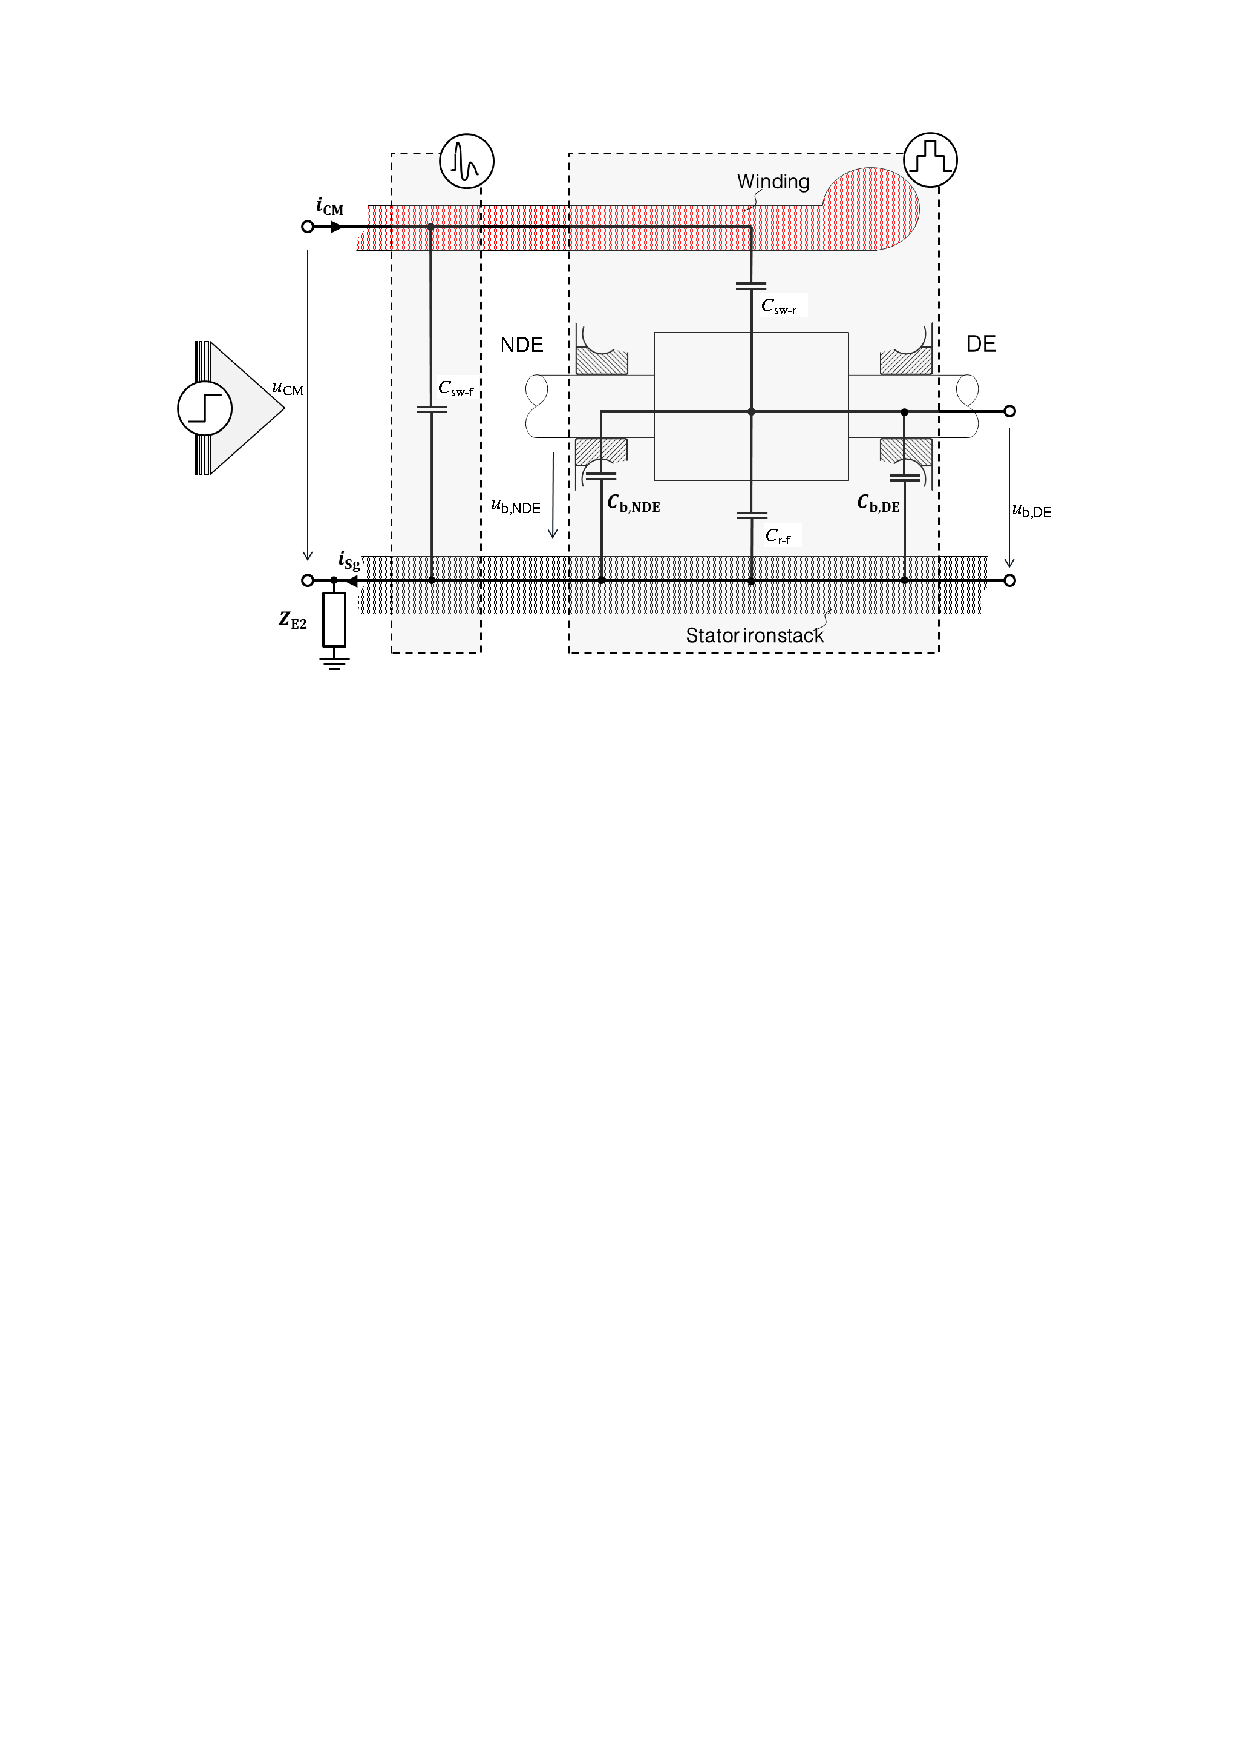
\includegraphics[width=\linewidth,height=0.65\textheight,keepaspectratio]{fig/lec02/Equivalent_capactive circuit.pdf}
            \caption{Equivalent capacitive circuit of the parasitic coupling paths.}
        \end{subfigure}
        \hfill
        \begin{subfigure}[b]{0.41\textwidth}
            \centering
            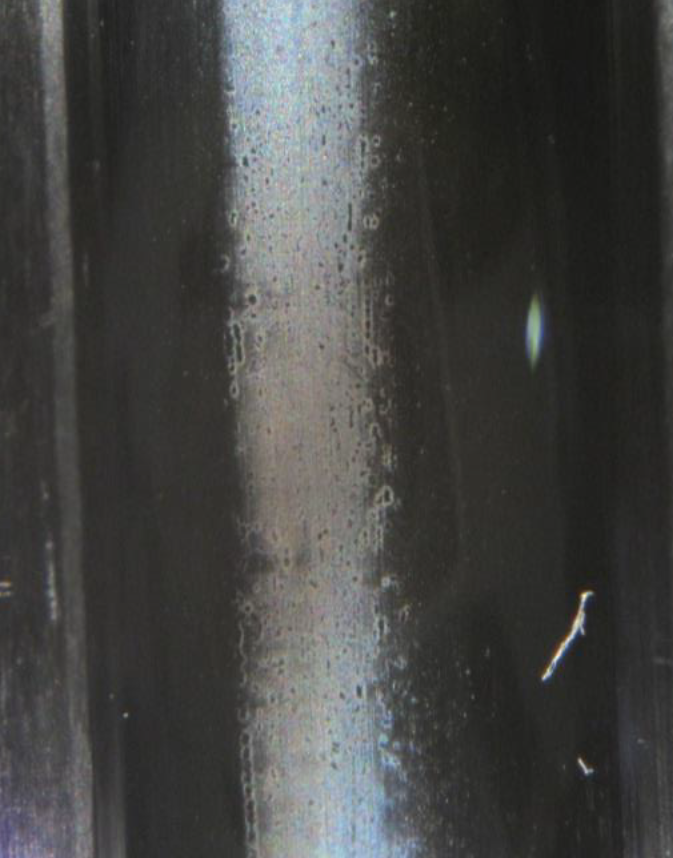
\includegraphics[width=\linewidth,height=0.65\textheight,keepaspectratio]{fig/lec02/Damaged_bearing.png}
            \caption{Bearing surface damage.}
        \end{subfigure}
        \caption{Inverter-induced bearing currents can lead to electrical discharge machining damage at the bearing surfaces (source: \href{https://tuprints.ulb.tu-darmstadt.de/id/eprint/19393}{TU Darmstadt}, \href{https://creativecommons.org/licenses/by/4.0/deed.en}{CC BY 4.0}).}
        \label{fig:inverter_induced_bearing_currents}
    \end{figure}
\end{frame}

%%%%%%%%%%%%%%%%%%%%%%%%%%%%%%%%%%%%%%%%%%%%%%%%%%%%%%%%%%%%%%%%%%
\subsection{Pulse width modulation}
%%%%%%%%%%%%%%%%%%%%%%%%%%%%%%%%%%%%%%%%%%%%%%%%%%%%%%%%%%%%%%%%%% % Inverter hardware and modulation techniques

%%%%%%%%%%%%%%%%%%%%%%%%%%%%%%%%%%%%%%%%%%%%%%%%%%%%%%%%%%%%%%%%%%
\section{Synchronous machine drives -- basic models and control concepts}
%%%%%%%%%%%%%%%%%%%%%%%%%%%%%%%%%%%%%%%%%%%%%%%%%%%%%%%%%%%%%%%%%%

%%%%%%%%%%%%%%%%%%%%%%%%%%%%%%%%%%%%%%%%%%%%%%%%%%%%%%%%%%%%%%%%%%
\subsection{Synchronous machine models}
%%%%%%%%%%%%%%%%%%%%%%%%%%%%%%%%%%%%%%%%%%%%%%%%%%%%%%%%%%%%%%%%%%

%%%%%%%%%%%%%%%%%%%%%%%%%%%%%%%%%%%%%%%%%%%%%%%%%%%%%%%%%%%%%
%% Synchronous machine (SM) rotor types %%
%%%%%%%%%%%%%%%%%%%%%%%%%%%%%%%%%%%%%%%%%%%%%%%%%%%%%%%%%%%%%
\begin{frame}
    \frametitle{Permanent magnet synchronous machine (PMSM) rotor types}
    \begin{figure}
        \centering
        \begin{subfigure}{0.49\textwidth}
            \centering
            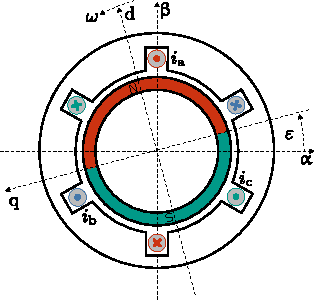
\includegraphics[width=0.8\textwidth]{fig/lec03/SPMSM.pdf}
            \caption{Surface-mounted PMSM(SPMSM)}
        \end{subfigure}
        \hfill
        \begin{subfigure}{0.49\textwidth}
            \centering
            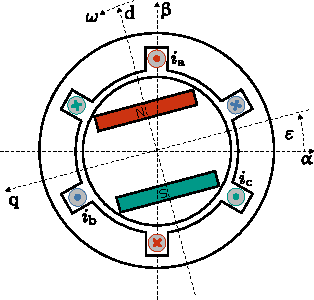
\includegraphics[width=0.8\textwidth]{fig/lec03/IPMSM.pdf}
            \caption{Interior PMSM (IPMSM)}
        \end{subfigure}
        \caption{Major rotor types of permanent magnet synchronous machines (PMSM) with dq reference frame axes aligned to the rotor flux produced by the permanent magnets}
        \label{fig:examples_PMSM_rotor}
    \end{figure}
\end{frame}

%%%%%%%%%%%%%%%%%%%%%%%%%%%%%%%%%%%%%%%%%%%%%%%%%%%%%%%%%%%%%
%% Summary: PMSM model in dq coordinates   %%
%%%%%%%%%%%%%%%%%%%%%%%%%%%%%%%%%%%%%%%%%%%%%%%%%%%%%%%%%%%%%
\begin{frame}
    \frametitle{PMSM model in dq coordinates}
    The most important equations of the PMSM model in the  dq coordinates are\footnote{A detailed derivation can be found in \href{https://github.com/IAS-Uni-Siegen/EMD_course}{Fundamentals of electrical machines and drives (EMD) course}.}:
    \begin{equation}
        \begin{alignedat}{4}
             &  & \mbox{Stator voltage:} &  & \quad\bm{u}_\mathrm{s,dq}( & t) &  & = R_\mathrm{s} \bm{i}_\mathrm{s,dq}(t)+ \omega(t)\bm{J}\bm{\psi}_\mathrm{s,dq}(t) + \nicefrac{\mathrm{d}}{\mathrm{d}t}\bm{\psi}_\mathrm{s,dq}(t), \\
            \onslide<2->{&  & \mbox{Stator flux linkage:} &  & \quad \bm{\psi}_\mathrm{s,dq}( & t) &  & = \bm{f}_{\psi_\mathrm{s}}(\bm{i}_\mathrm{s,dq}(t), \psi_\mathrm{PM}),}                                                      \\\onslide<3->{
                                                                                                                                                                                                                                                          &  & \mbox{Torque:}              &  & \quad T(                       & t) &  & = \nicefrac{3}{2} p (\bm{i}_\mathrm{s,dq}(t))\T\bm{J}\bm{\psi}_\mathrm{s,dq}(t)}
        \end{alignedat}
        \label{eq:basic_PMSM_model_set}
    \end{equation}
    \onslide<4->{with the further signals and parameters:
            \begin{equation*}
                \begin{aligned}
                    \bm{i}_\mathrm{s,dq}: \text{stator current},                                                              &
                    \qquad \psi_\mathrm{PM}  : \text{permanent magnet flux linkage},                                            \\
                    R_\mathrm{s}:                                                          \text{stator winding resistances}, &
                    \qquad \bm{f}_{\psi_\mathrm{s}} : \text{stator flux linkage function},                                      \\
                    p                                           : \text{pole pair number},                                    &
                    \qquad \omega = p\omega_\mathrm{me}                   : \text{electrical angular velocity,}                 \\
                    \bm{J}: \text{90° rotation matrix, cf. \eqref{eq:J_rotation}}.                                            &
                \end{aligned}
            \end{equation*}}
\end{frame}

%%%%%%%%%%%%%%%%%%%%%%%%%%%%%%%%%%%%%%%%%%%%%%%%%%%%%%%%%%%%%
%% Flux saturation motor cross section %%
%%%%%%%%%%%%%%%%%%%%%%%%%%%%%%%%%%%%%%%%%%%%%%%%%%%%%%%%%%%%%

\begin{frame}
    \frametitle{Flux saturation in electric machines}
    \begin{figure}
        \centering
        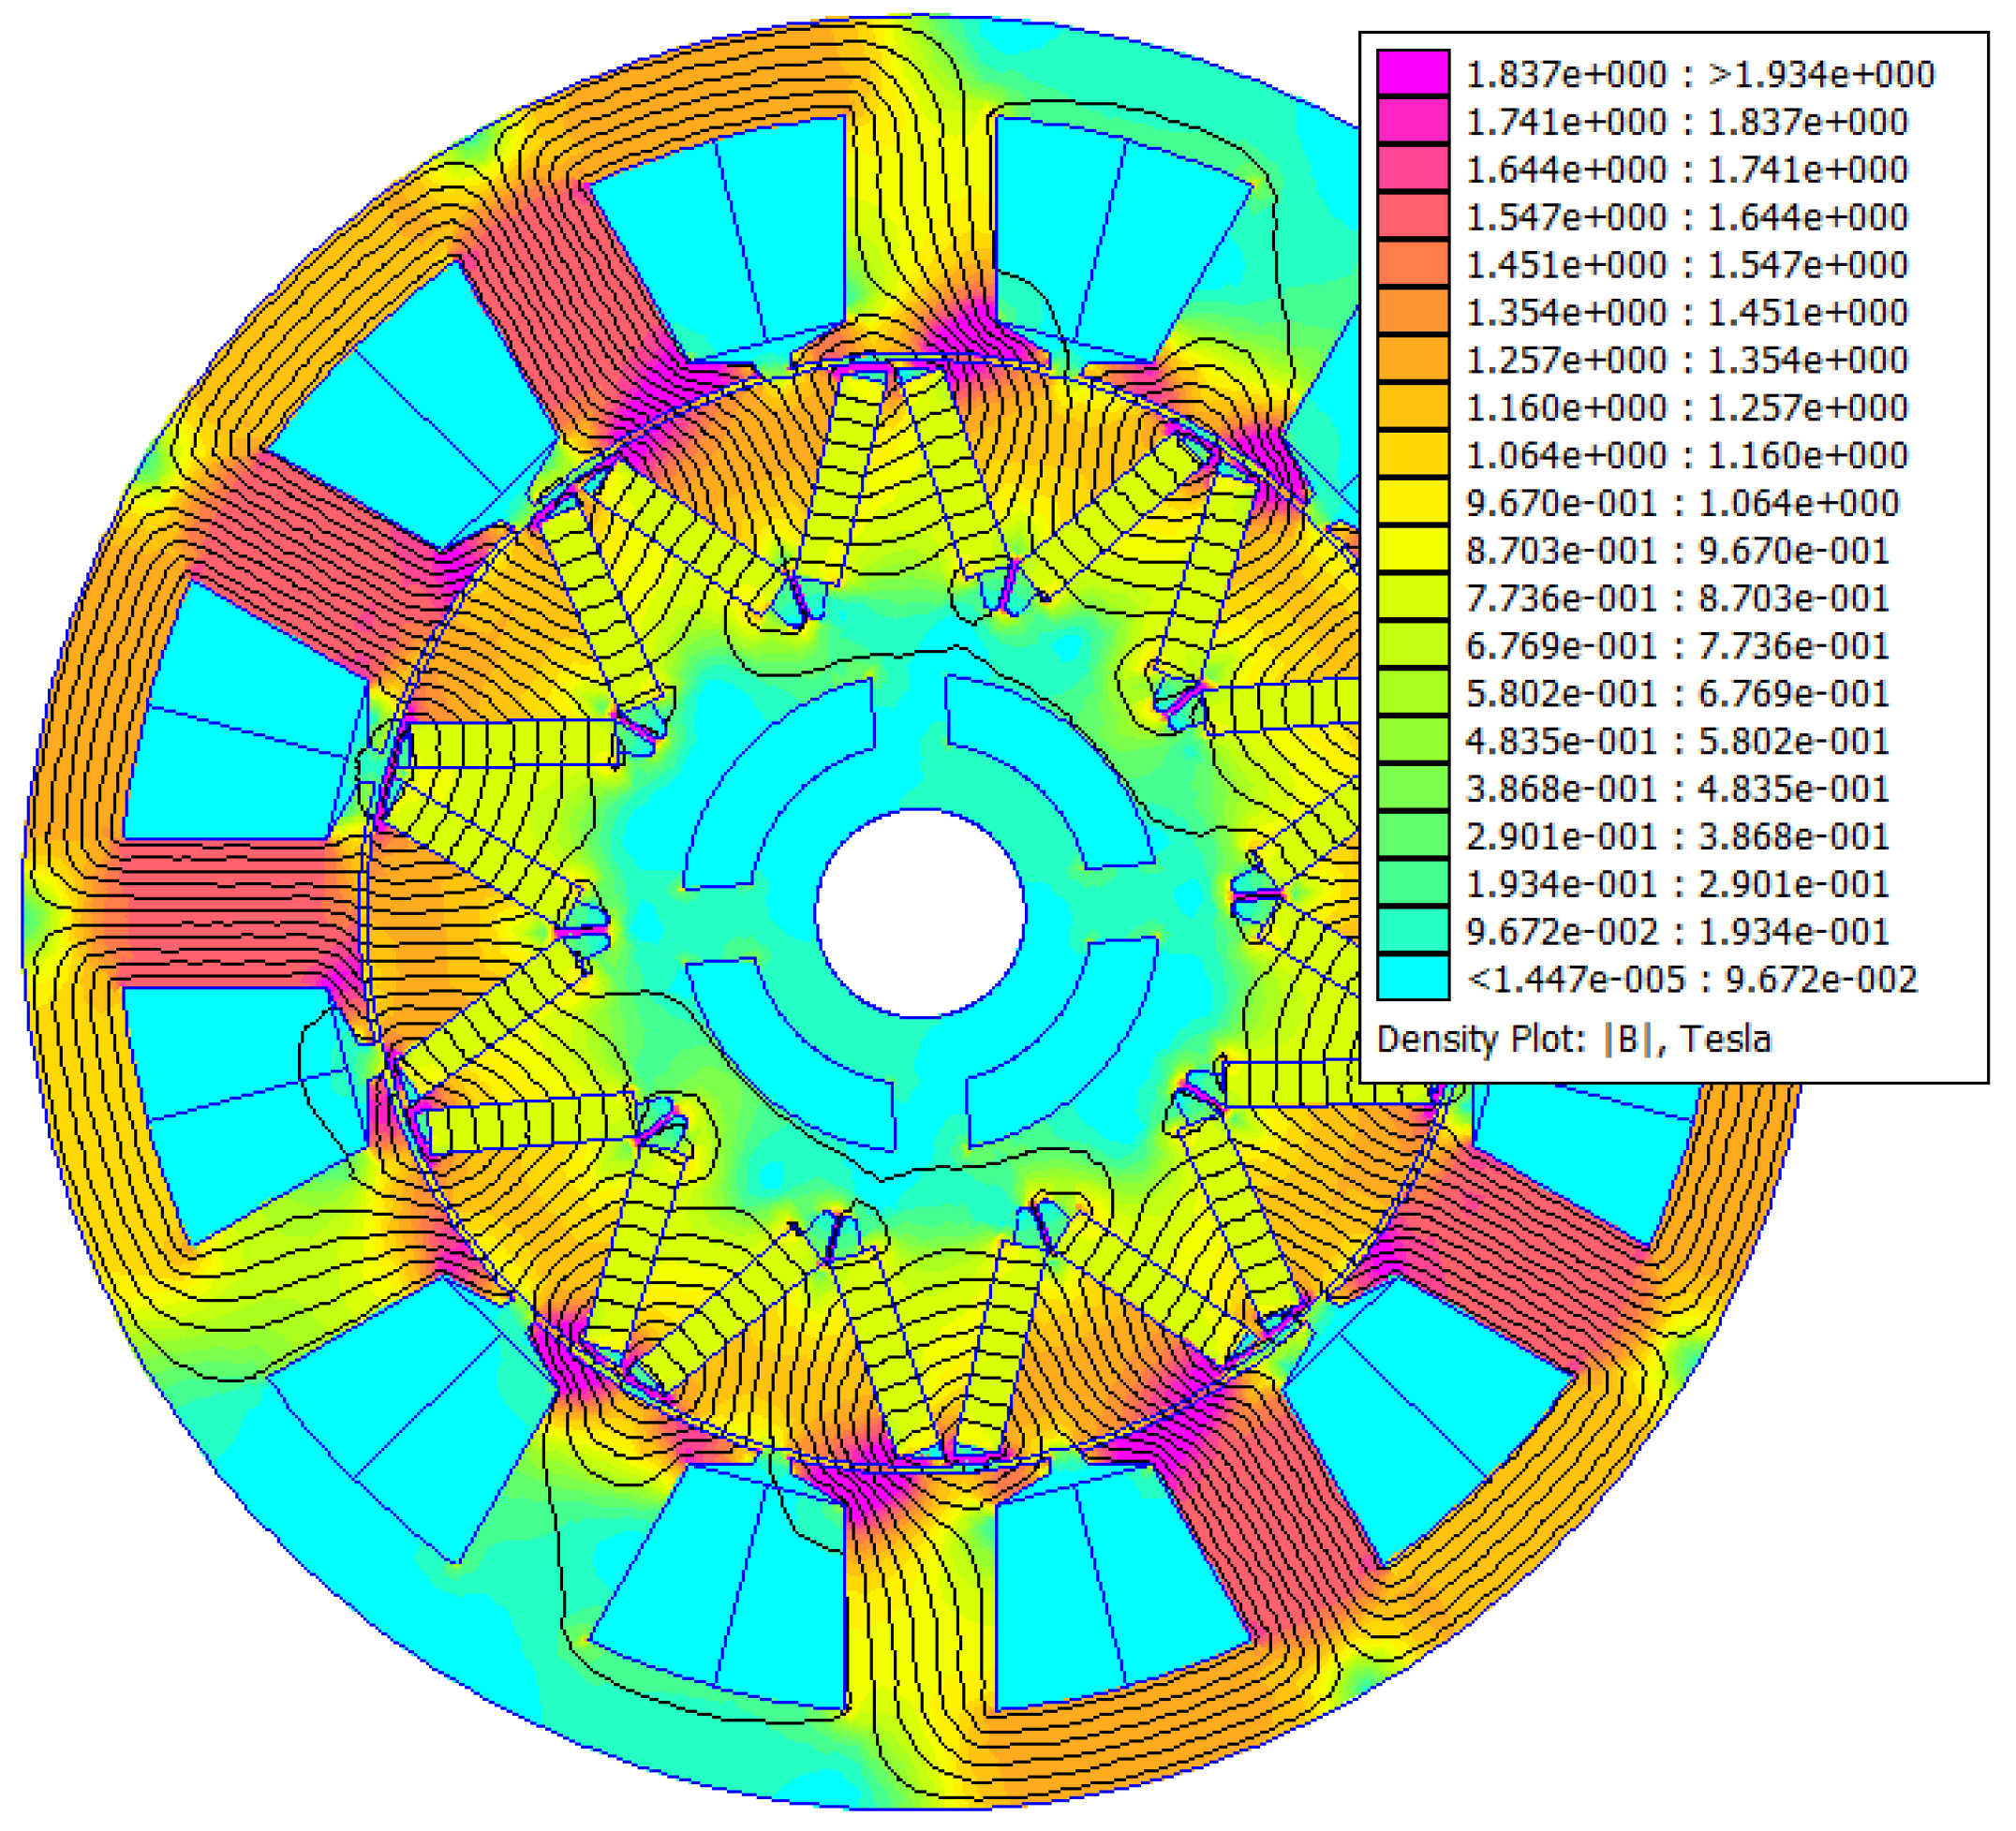
\includegraphics[height=0.75\textheight]{fig/lec03/IPMSM_flux_density_example.png}
        \caption{Exemplary cross-section of an IPMSM with flux density distribution (source: \href{https://www.mdpi.com/2076-3417/12/23/11956}{10.3390/app122311956}, \href{https://creativecommons.org/licenses/by/4.0/deed.en}{CC BY 4.0})}
        \label{fig:motor_cross_section}
    \end{figure}
\end{frame}

%%%%%%%%%%%%%%%%%%%%%%%%%%%%%%%%%%%%%%%%%%%%%%%%%%%%%%%%%%%%%
%% Flux saturation in electric machines (cont.) %%
%%%%%%%%%%%%%%%%%%%%%%%%%%%%%%%%%%%%%%%%%%%%%%%%%%%%%%%%%%%%%
\begin{frame}
    \frametitle{Flux saturation in electric machines (cont.)}
    \begin{figure}
        \centering
        \movie[height=0.74\textheight]{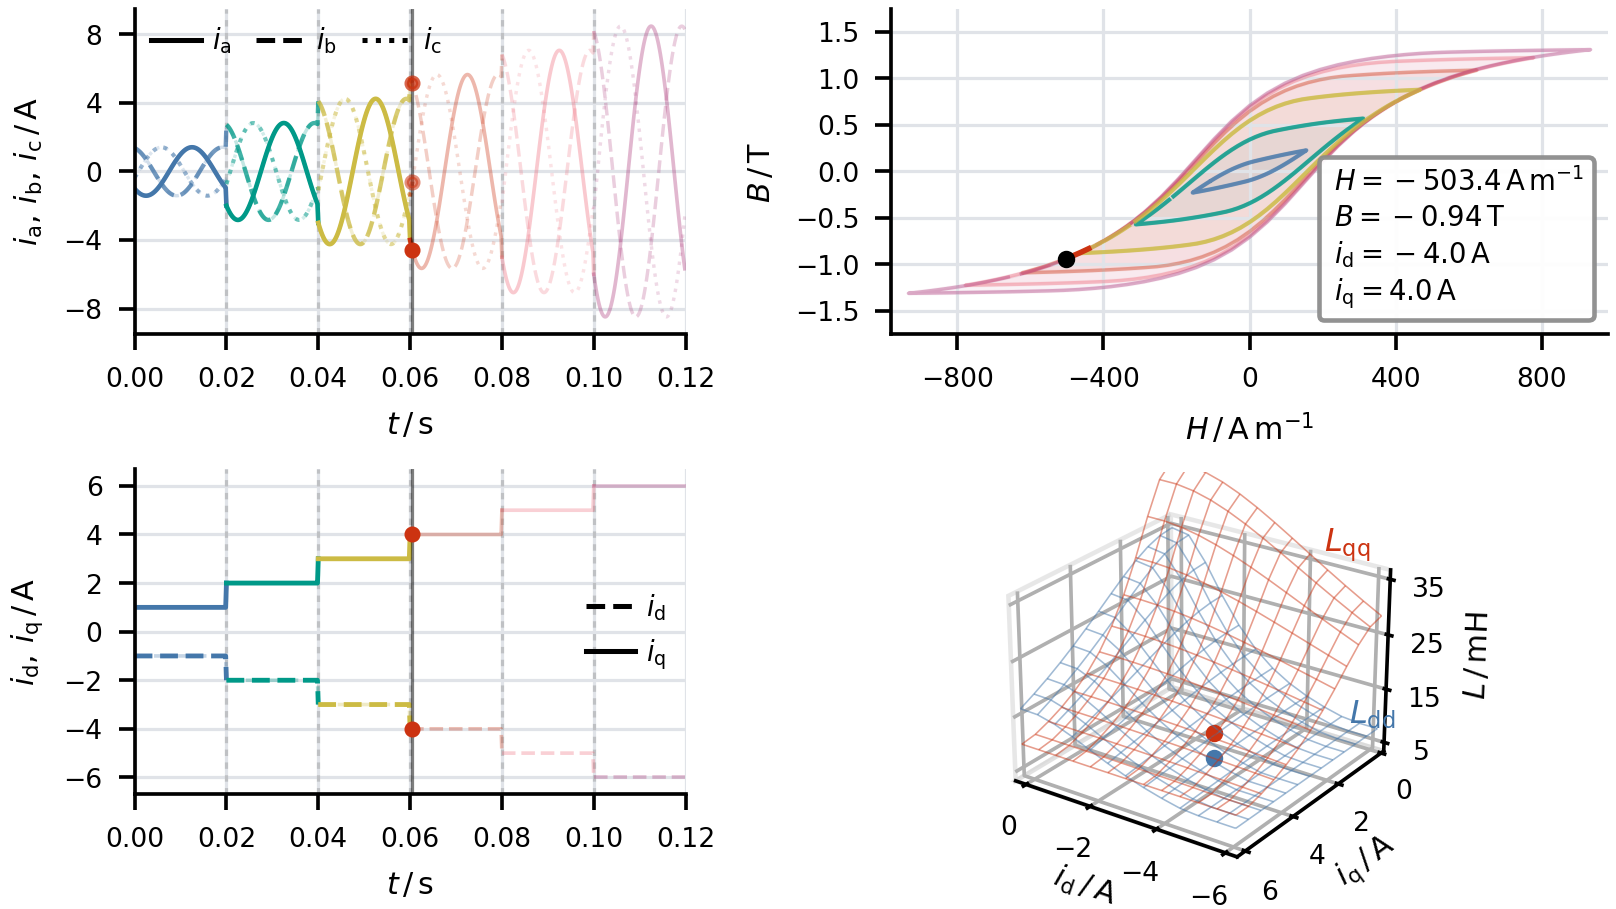
\includegraphics[height=0.678\textheight]{fig/lec03/PMSM_Saturation_BH_Example.png}}{fig/lec03/PMSM_Saturation_BH_Example.mp4}
        \caption{Illustrative and simplified representation of flux saturation in a PMSM based on the \href{https://en.wikipedia.org/wiki/Jiles\%E2\%80\%93Atherton_model}{Jiles-Atherton} B-H curve model (animation)}
        \label{fig:pmsm_saturation_bh_animation}
    \end{figure}
\end{frame}

%%%%%%%%%%%%%%%%%%%%%%%%%%%%%%%%%%%%%%%%%%%%%%%%%%%%%%%%%%%%%
%% Flux saturation: apparent vs.\ differential inductance %%
%%%%%%%%%%%%%%%%%%%%%%%%%%%%%%%%%%%%%%%%%%%%%%%%%%%%%%%%%%%%%
\begin{frame}
    \frametitle{Flux linkage saturation: apparent vs.\ differential inductance}
    \begin{figure}
        \centering
        \begin{tikzpicture}
            \begin{axis}[
                    width=0.72\textwidth,
                    height=0.62\textheight,
                    xlabel={$i$},
                    ylabel={$\psi,\,  L,\,  L_{\mathrm{app}}$},
                    xmin=-0.3, xmax=10.8,
                    ymin=-0.08, ymax=3.40,
                    axis lines=left,
                    clip=false,
                    xtick=\empty,
                    ytick=\empty,
                    xlabel style = {at={(axis description cs:1,0)},anchor=north east},
                    ylabel style = {at={(axis description cs:0,1)},anchor=south east},
                    legend style={at={(1.02,0.98)}, anchor=north west,
                            draw=black, fill=white, font=\small,
                            legend cell align=left,
                            inner xsep=6pt, inner ysep=4pt},
                ]
                %-- Flux saturation curve: psi(i) = 3*tanh(i/3) --%
                \addplot[black, very thick, smooth, domain=0:10.4, samples=120]
                {3*tanh(x/3)};
                \addlegendentry{$\psi$}

                %-- Differential inductance: L = d(psi)/di = 1/cosh^2(i/3) --%

                \addplot[signalalpha, thick, smooth, domain=0.01:10.4, samples=120, visible on=<3->]
                {1/(cosh(x/3)^2)};
                \addlegendentry[visible on=<3->]{$L = \nicefrac{\mathrm{d}\psi}{\mathrm{d}i}$}

                %-- Apparent inductance: L_app = psi/i = 3/i * tanh(i/3) --%

                \addplot[signaldelta, thick, smooth, domain=0.10:10.4, samples=120, visible on=<2->]
                {3/x * tanh(x/3)};
                \addlegendentry[visible on=<2->]{$L_{\mathrm{app}} = \nicefrac{\psi}{i}$}

                %-- Tangent lines at operating points (signalalpha, dashed) --%

                % i1=1.5: psi1=3*tanh(0.5)=1.3863, L1=1/cosh(0.5)^2=0.7864
                \addplot[signalalpha, dashed, thick, domain=0:3.2, forget plot, visible on=<3->]
                {0.7864*(x-1.5) + 1.3863};
                % i2=4: psi2=3*tanh(4/3)=2.6141, L2=1/cosh(4/3)^2=0.2604
                \addplot[signalalpha, dashed, thick, domain=1.3:6.5, forget plot, visible on=<3->]
                {0.2604*(x-4) + 2.6141};
                % i3=7: psi3=3*tanh(7/3)=2.9447, L3=1/cosh(7/3)^2=0.0387
                \addplot[signalalpha, dashed, thick, domain=4.8:9.2, forget plot, visible on=<3->]
                {0.0387*(x-7) + 2.9447};

                %-- Secant lines from origin (signaldelta, dotted) --%

                % L_app1 = 1.3863/1.5 = 0.9242
                \addplot[signaldelta, dotted, thick, domain=0:2.0, forget plot, visible on=<2->]
                {0.9242*x};
                % L_app2 = 2.6141/4 = 0.6535
                \addplot[signaldelta, dotted, thick, domain=0:4.8, forget plot, visible on=<2->]
                {0.6535*x};
                % L_app3 = 2.9447/7 = 0.4207
                \addplot[signaldelta, dotted, thick, domain=0:7.8, forget plot, visible on=<2->]
                {0.4207*x};

                %-- Operating points --%
                \addplot[black, mark=*, mark size=2.5pt, only marks, forget plot]
                coordinates {(1.5, 1.3863) (4, 2.6141) (7, 2.9447)};

                %-- Operating point labels --%
                \node[above left, font=\small] at (axis cs:1.5, 1.3863)
                {$(i_1,\psi_1)$};
                \node[above left, font=\small] at (axis cs:4, 2.6141)
                {$(i_2,\psi_2)$};
                \node[above, font=\small] at (axis cs:7, 2.9447)
                {$(i_3,\psi_3)$};
            \end{axis}
        \end{tikzpicture}
        \caption{Nonlinear flux linkage $\psi(i)$ with the differential inductance $L$ (slope of the tangent) and the apparent inductance $L_{\mathrm{app}}$ (slope of the secant from the origin) -- inspired by \href{https://www.researchgate.net/publication/384459015_A_generic_approach_to_modern_electrical_drives_Tutorial_at_PEMC_2024}{10.13140/RG.2.2.33279.01443}}
        \label{fig:flux_saturation}
    \end{figure}
\end{frame}

%%%%%%%%%%%%%%%%%%%%%%%%%%%%%%%%%%%%%%%%%%%%%%%%%%%%%%%%%%%%%
%% PMSM current-to-flux maps   %%
%%%%%%%%%%%%%%%%%%%%%%%%%%%%%%%%%%%%%%%%%%%%%%%%%%%%%%%%%%%%%
\begin{frame}
    \frametitle{PMSM current-to-flux maps: nonlinear magnetic saturation}

    \begin{figure}
        \begin{tikzpicture}
            \begin{groupplot}[
                    group style={group size=2 by 1, horizontal sep=2.5cm},
                    width=7cm,
                    height=6.25cm,
                    view={-45}{24},
                    xlabel={$i_{\mathrm{d}}\,/\,\mathrm{A}$},
                    ylabel={$i_{\mathrm{q}}\,/\,\mathrm{A}$},
                    xmin=-250, xmax=0,
                    ymin=-250, ymax=250,
                    enlargelimits=false,
                    xlabel style={yshift=2ex},
                    ylabel style={yshift=2ex},
                    xtick={-200,-100,0},
                    ytick={-200,-100, 0,100,200},
                    grid=major,
                    grid style={line width=.1pt, draw=gray!40},
                    tick label style={font=\small},
                    label style={font=\normalsize},
                    zlabel style={font=\normalsize},
                    title style={font=\normalsize},
                ]
                \nextgroupplot[
                    zlabel={$\psi_{\mathrm{d}}\,/\,\mathrm{mVs}$},
                    ztick={0, 25, 50},
                ]
                \addplot3[
                    surf,
                    mesh/rows=26,
                    mesh/cols=14,
                    draw=black,
                    shader=flat,
                    fill=signalalpha,
                    opacity=0.78,
                ]
                table[x=id,y=iq,z expr=1000*\thisrow{psi_d}] {fig/lec03/PMSM_flux_maps.dat};

                \nextgroupplot[
                    zlabel={$\psi_{\mathrm{q}}\,/\,\mathrm{mVs}$},
                ]
                \addplot3[
                    surf,
                    mesh/rows=26,
                    mesh/cols=14,
                    draw=black,
                    shader=flat,
                    fill=signalalpha,
                    opacity=0.78,
                ]
                table[x=id,y=iq,z expr=1000*\thisrow{psi_q}] {fig/lec03/PMSM_flux_maps.dat};
            \end{groupplot}
        \end{tikzpicture}
        \caption{Exemplary current-to-flux maps for a \SI{68}{\kilo\watt} PMSM (derived from \href{https://ieeexplore.ieee.org/document/10098161}{10.1109/TPEL.2023.3265705}, \href{https://creativecommons.org/licenses/by/4.0/deed.en}{CC BY 4.0})}
        \label{fig:flux_maps_BRUSA}
    \end{figure}
\end{frame}

%%%%%%%%%%%%%%%%%%%%%%%%%%%%%%%%%%%%%%%%%%%%%%%%%%%%%%%%%%%%%
%% PMSM current-to-flux maps (cont.): differential inductances   %%
%%%%%%%%%%%%%%%%%%%%%%%%%%%%%%%%%%%%%%%%%%%%%%%%%%%%%%%%%%%%%
\begin{frame}
    \frametitle{PMSM current-to-flux maps (cont.): differential inductances}
    \begin{figure}
        \begin{tikzpicture}
            \begin{groupplot}[
                    group style={group size=2 by 2, horizontal sep=2.55cm, vertical sep=0.6cm},
                    width=0.4\textwidth,
                    height=0.285\textwidth,
                    xlabel={$i_\mathrm{d} / \mathrm{A}$},
                    ylabel={$i_\mathrm{q} / \mathrm{A}$},
                    xmin=-250, xmax=0,
                    ymin=-250, ymax=250,
                    xlabel style={yshift=2ex},
                    ylabel style={yshift=2ex},
                    view={-45}{40},
                    enlargelimits=false,
                    grid=major,
                    grid style={line width=.1pt, draw=gray!40},
                    minor tick num=1,
                    tick label style={font=\small},
                    label style={font=\small},
                    title style={font=\small},
                ]
                \nextgroupplot[
                    zlabel={$L_\mathrm{dd}/ \mathrm{mH}$}
                ]
                \addplot3[surf,
                    mesh/rows=26,
                    mesh/cols=14,
                    shader=flat,
                    draw=black,
                    fill=signalalpha,
                    opacity=0.78,]
                table[x=id, y=iq, z expr=1000*\thisrow{L_dd}] {fig/lec03/PMSM_diff_inductance_maps.dat};

                \nextgroupplot[
                    zlabel={$L_\mathrm{dq} / \mathrm{mH}$}
                ]
                \addplot3[surf,
                    mesh/rows=26,
                    mesh/cols=14,
                    shader=flat,
                    draw=black,
                    fill=signalalpha,
                    opacity=0.78,]
                table[x=id, y=iq, z expr=1000*\thisrow{L_dq}] {fig/lec03/PMSM_diff_inductance_maps.dat};
                \nextgroupplot[
                    zlabel={$L_\mathrm{qd}/ \mathrm{mH}$},
                ]
                \addplot3[surf,
                    mesh/rows=26,
                    mesh/cols=14,
                    shader=flat,
                    draw=black,
                    fill=signalalpha,
                    opacity=0.78,]
                table[x=id, y=iq, z expr=1000*\thisrow{L_qd}] {fig/lec03/PMSM_diff_inductance_maps.dat};

                \nextgroupplot[
                    zlabel={$L_\mathrm{qq}/ \mathrm{mH}$},
                ]
                \addplot3[surf,
                    mesh/rows=26,
                    mesh/cols=14,
                    shader=flat,
                    draw=black,
                    fill=signalalpha,
                    opacity=0.78,]
                table[x=id, y=iq, z expr=1000*\thisrow{L_qq}] {fig/lec03/PMSM_diff_inductance_maps.dat};
            \end{groupplot}
        \end{tikzpicture}
        \caption{Exemplary differential inductance maps derived from \figref{fig:flux_maps_BRUSA}}
        \label{fig:inductance_maps_BRUSA}
    \end{figure}
\end{frame}







%%%%%%%%%%%%%%%%%%%%%%%%%%%%%%%%%%%%%%%%%%%%%%%%%%%%%%%%%%%%%
%% Nonlinear PMSM flux linkage model and inductances %%
%%%%%%%%%%%%%%%%%%%%%%%%%%%%%%%%%%%%%%%%%%%%%%%%%%%%%%%%%%%%%
\begin{frame}
    \frametitle{Nonlinear PMSM flux linkage model and inductances}
    Consider the following nonlinear flux linkage model in dq coordinates for a PMSM:
    \begin{equation}
        \bm{\psi}_\mathrm{s,dq}(t) = \begin{bmatrix}
            \psi_\mathrm{s,d}(t) \\
            \psi_\mathrm{s,q}(t)
        \end{bmatrix} = \bm{f}_{\psi_\mathrm{s}}(\bm{i}_\mathrm{s,dq}(t)).
        \label{eq:nonlinear_flux_function_PMSM}
    \end{equation}
    \onslide<2->{Applying the chain rule yields the time derivative}
    \begin{equation}
        \begin{split}
            \onslide<2->{\frac{\mathrm{d}}{\mathrm{d}t}\bm{\psi}_\mathrm{s,dq}(t)
                               = \underbrace{\frac{\partial \bm{f}_{\psi_\mathrm{s}}}{\partial \bm{i}_\mathrm{s,dq}}}_{\displaystyle=\,\bm{L}(\bm{i}_\mathrm{s,dq})}
                               \frac{\mathrm{d}}{\mathrm{d}t}\bm{i}_\mathrm{s,dq}(t) &} \onslide<3->{= \begin{bmatrix}
                                                                                                               \text{\makebox[\widthof{$L_\mathrm{dd}(\bm{i}_\mathrm{s,dq})$}][c]{$\dfrac{\partial \psi_\mathrm{s,d}}{\partial i_\mathrm{s,d}}$}} &
                                                                                                               \text{\makebox[\widthof{$L_\mathrm{dq}(\bm{i}_\mathrm{s,dq})$}][c]{$\dfrac{\partial \psi_\mathrm{s,d}}{\partial i_\mathrm{s,q}}$}}   \\[1.5ex]
                                                                                                               \text{\makebox[\widthof{$L_\mathrm{qd}(\bm{i}_\mathrm{s,dq})$}][c]{$\dfrac{\partial \psi_\mathrm{s,q}}{\partial i_\mathrm{s,d}}$}} &
                                                                                                               \text{\makebox[\widthof{$L_\mathrm{qq}(\bm{i}_\mathrm{s,dq})$}][c]{$\dfrac{\partial \psi_\mathrm{s,q}}{\partial i_\mathrm{s,q}}$}}
                                                                                                           \end{bmatrix}\frac{\mathrm{d}}{\mathrm{d}t}\bm{i}_\mathrm{s,dq}(t)} \\ & \onslide<4->{= \begin{bmatrix}
                                                                                                                                                                                                           L_\mathrm{dd}(\bm{i}_\mathrm{s,dq}) & L_\mathrm{dq}(\bm{i}_\mathrm{s,dq}) \\[1.6ex]
                                                                                                                                                                                                           L_\mathrm{qd}(\bm{i}_\mathrm{s,dq}) & L_\mathrm{qq}(\bm{i}_\mathrm{s,dq})
                                                                                                                                                                                                       \end{bmatrix}\frac{\mathrm{d}}{\mathrm{d}t}\bm{i}_\mathrm{s,dq}(t),}
        \end{split}
    \end{equation}
    \onslide<4->{where the \hl{differential inductance matrix} $\bm{L}(\bm{i}_\mathrm{s,dq})$ is the Jacobian of $\bm{f}_{\psi_\mathrm{s}}$ with respect to $\bm{i}_\mathrm{s,dq}$.}
\end{frame}

%%%%%%%%%%%%%%%%%%%%%%%%%%%%%%%%%%%%%%%%%%%%%%%%%%%%%%%%%%%%%
%% Nonlinear PMSM flux linkage model and inductances (cont) %%
%%%%%%%%%%%%%%%%%%%%%%%%%%%%%%%%%%%%%%%%%%%%%%%%%%%%%%%%%%%%%
\begin{frame}
    \frametitle{Nonlinear PMSM flux linkage model and inductances (cont.)}
    Representing the nonlinear flux linkage model \eqref{eq:nonlinear_flux_function_PMSM} based on the \hl{apparent inductance matrix} $\bm{L}_{\mathrm{app}}(\bm{i}_\mathrm{s,dq})$ yields
    \begin{equation}
        \bm{\psi}_\mathrm{s,dq}(t) = \bm{L}_{\mathrm{app}}(\bm{i}_\mathrm{s,dq}(t))\bm{i}_\mathrm{s,dq}(t) + \bm{\psi}_\mathrm{PM}
    \end{equation}\pause
    with
    \begin{equation}
        \bm{L}_{\mathrm{app}}(\bm{i}_\mathrm{s,dq}) = \begin{bmatrix}
            L_{\mathrm{dd,app}}(i_\mathrm{s,d})                 & L_{\mathrm{dq,app}}(i_\mathrm{s,d}, i_\mathrm{s,q}) \\[1.5ex]
            L_{\mathrm{qd,app}}(i_\mathrm{s,d}, i_\mathrm{s,q}) & L_{\mathrm{qq,app}}(i_\mathrm{s,q})
        \end{bmatrix}, \quad \bm{\psi}_\mathrm{PM} = \begin{bmatrix}
            \psi_\mathrm{PM} \\[1.5ex]
            0
        \end{bmatrix}.
    \end{equation}\pause
    Here, the following can be noted:
    \begin{itemize}
        \item Main diagonal elements of $\bm{L}_{\mathrm{app}}$ depend only on the respective current component since otherwise the current-to-flux maps would be not unique (overdetermined system).\pause
        \item Since the apparent inductance matrix represents the absolute flux linkage change due to the stator currents, the PM flux linkage $\bm{\psi}_\mathrm{PM}$ is explicitly included in the model.\pause
        \item Since the apparent inductance representation is less elegant than the original flux function $\bm{f}_{\psi_\mathrm{s}}$ and partly ambiguous, it is not commonly used for control-oriented modeling of PMSMs.
    \end{itemize}
\end{frame}

%%%%%%%%%%%%%%%%%%%%%%%%%%%%%%%%%%%%%%%%%%%%%%%%%%%%%%%%%%%%%
%% Current differential equations of the nonlinear PMSM model %%
%%%%%%%%%%%%%%%%%%%%%%%%%%%%%%%%%%%%%%%%%%%%%%%%%%%%%%%%%%%%%
\begin{frame}
    \frametitle{Current differential equations of the nonlinear PMSM model}
    Utilizing the differential inductance concept, the \hl{current differential equation} can be derived as
    \begin{equation}
        \begin{split}
            \bm{u}_\mathrm{s,dq}(t) & = R_\mathrm{s} \bm{i}_\mathrm{s,dq}(t)+ \omega(t)\bm{J}\bm{\psi}_\mathrm{s,dq}(t) + \nicefrac{\mathrm{d}}{\mathrm{d}t}\bm{\psi}_\mathrm{s,dq}(t) \\ \onslide<2->{&= R_\mathrm{s} \bm{i}_\mathrm{s,dq}(t)+ \omega(t)\bm{J}\bm{f}_{\psi_\mathrm{s}}(\bm{i}_\mathrm{s,dq}(t)) + \bm{L}(\bm{i}_\mathrm{s,dq})\frac{\mathrm{d}}{\mathrm{d}t}\bm{i}_\mathrm{s,dq}(t)} \\
            \onslide<3->{\Leftrightarrow  \frac{\mathrm{d}}{\mathrm{d}t}\bm{i}_\mathrm{s,dq}(t) & = \bm{L}^{-1}(\bm{i}_\mathrm{s,dq})\left[\bm{u}_\mathrm{s,dq}(t)- R_\mathrm{s} \bm{i}_\mathrm{s,dq}(t)- \omega(t)\bm{J}\bm{f}_{\psi_\mathrm{s}}(\bm{i}_\mathrm{s,dq}(t))\right].}
        \end{split}
    \end{equation}
    \begin{itemize}
        \item<4-> The model $\bm{f}_{\psi_\mathrm{s}}$ can be implemented as look-up table (LUT) plus interpolation or as a function approximator (e.g., neural network, polynomial, prototype functions).
        \item<5-> Inverse $\bm{L}^{-1}(\bm{i}_\mathrm{s,dq})$ can be precomputed offline based on finite difference or analytical differentiation depending on the implementation of $\bm{f}_{\psi_\mathrm{s}}$.
        \item<6-> Alternatively, one can integrate the flux ODE \eqref{eq:basic_PMSM_model_set} and then compute  $\bm{i}_\mathrm{s,dq}=\bm{f}_{\psi_\mathrm{s}}^{-1}(\bm{\psi}_\mathrm{s,dq})$.
    \end{itemize}
\end{frame}

%%%%%%%%%%%%%%%%%%%%%%%%%%%%%%%%%%%%%%%%%%%%%%%%%%%%%%%%%%%%%
%% Current differential equations of the nonlinear PMSM model %%
%%%%%%%%%%%%%%%%%%%%%%%%%%%%%%%%%%%%%%%%%%%%%%%%%%%%%%%%%%%%%
\begin{frame}
    \frametitle{Linear PMSM model with constant inductances}
    Applying the \hl{first-order Taylor expansion} to the nonlinear flux function $\bm{f}_{\psi_\mathrm{s}}$ around some operating point (typically the origin $\bm{i}_\mathrm{s,dq}=\bm{0}$) yields the \hl{linear PMSM flux model}
    \begin{equation}
        \bm{\psi}_\mathrm{s,dq}(t)  \approx \underbrace{\bm{f}_{\psi_\mathrm{s}}(\bm{0})\vphantom{\frac{\partial \bm{f}_{\psi_\mathrm{s}}}{\partial \bm{i}_\mathrm{s,dq}}\bigg|_{\bm{i}_\mathrm{s,dq}=\bm{0}}}}_{\displaystyle=\bm{\psi}_\mathrm{PM}} + \underbrace{\frac{\partial \bm{f}_{\psi_\mathrm{s}}}{\partial \bm{i}_\mathrm{s,dq}}\bigg|_{\bm{i}_\mathrm{s,dq}=\bm{0}}}_{\displaystyle=\,\bm{L}_0}\bm{i}_\mathrm{s,dq}(t)  \onslide<2->{= \begin{bmatrix}
                    \psi_{\mathrm{PM}} \\
                    0
                \end{bmatrix} + \begin{bmatrix}
                    L_{\mathrm{dd},0} & L_{\mathrm{dq},0} \\
                    L_{\mathrm{qd},0} & L_{\mathrm{qq},0}
                \end{bmatrix}\bm{i}_\mathrm{s,dq}(t)}.
    \end{equation}
    \onslide<3->{With this linear flux model, the current ODE simplifies to}
    \begin{equation}
        \begin{split}
            \onslide<3->{\bm{u}_\mathrm{s,dq}(t)                                                & = R_\mathrm{s} \bm{i}_\mathrm{s,dq}(t)+ \omega(t)\bm{J}\left[\bm{\psi}_\mathrm{PM} + \bm{L}_0 \bm{i}_\mathrm{s,dq}(t)\right] + \bm{L}_0\frac{\mathrm{d}}{\mathrm{d}t}\bm{i}_\mathrm{s,dq}(t)} \\
            \onslide<4->{\Leftrightarrow  \frac{\mathrm{d}}{\mathrm{d}t}\bm{i}_\mathrm{s,dq}(t) & = \bm{L}_0^{-1}\left[\bm{u}_\mathrm{s,dq}(t)- R_\mathrm{s} \bm{i}_\mathrm{s,dq}(t)- \omega(t)\bm{J}\left(\bm{\psi}_\mathrm{PM} + \bm{L}_0 \bm{i}_\mathrm{s,dq}(t)\right)\right].}
        \end{split}
    \end{equation}
    \onslide<5->{And the torque expressions results in
            \begin{equation}
                T(t) = \frac{3}{2}p\left[\psi_\mathrm{PM} i_\mathrm{s,q}(t) + (L_{\mathrm{dd},0}-L_{\mathrm{qq},0})i_\mathrm{s,d}(t)i_\mathrm{s,q}(t) + L_{\mathrm{dq},0} i_\mathrm{s,d}^2(t) - L_{\mathrm{qd},0} i_\mathrm{s,q}^2(t)\right].
            \end{equation}}
\end{frame}

%%%%%%%%%%%%%%%%%%%%%%%%%%%%%%%%%%%%%%%%%%%%%%%%%%%%%%%%%%%%%
%% Current differential equations of the nonlinear PMSM model %%
%%%%%%%%%%%%%%%%%%%%%%%%%%%%%%%%%%%%%%%%%%%%%%%%%%%%%%%%%%%%%
\begin{frame}
    \frametitle{Linear PMSM model with constant inductances (cont.)}
    As can be seen from \figref{fig:inductance_maps_BRUSA} the off-diagonal inductance terms $L_{\mathrm{dq},0}$ and $L_{\mathrm{qd},0}$ are much smaller than the main diagonal terms $L_{\mathrm{dd},0}$ and $L_{\mathrm{qq},0}$. \pause Thus, by further simplification
    $$
        L_{\mathrm{dq},0} \approx L_{\mathrm{qd},0} \approx 0
    $$\pause
    we obtain the following current ODE
    \begin{equation}
        \frac{\mathrm{d}}{\mathrm{d}t}\bm{i}_\mathrm{s,dq}(t) = \begin{bmatrix}
            L_{\mathrm{dd},0}^{-1} & 0                      \\
            0                      & L_{\mathrm{qq},0}^{-1}
        \end{bmatrix}\left[\bm{u}_\mathrm{s,dq}(t)- R_\mathrm{s} \bm{i}_\mathrm{s,dq}(t)- \omega(t)\bm{J}\left(\bm{\psi}_\mathrm{PM} + \begin{bmatrix}
                L_{\mathrm{dd},0} & 0                 \\
                0                 & L_{\mathrm{qq},0}
            \end{bmatrix} \bm{i}_\mathrm{s,dq}(t)\right)\right].
    \end{equation}\pause
    and torque expression
    \begin{equation}
        T(t) = \frac{3}{2}p\left[\psi_\mathrm{PM} i_\mathrm{s,q}(t) + (L_{\mathrm{dd},0}-L_{\mathrm{qq},0})i_\mathrm{s,d}(t)i_\mathrm{s,q}(t)\right].
    \end{equation}\pause
    This is the \hl{standard linear model for IPMSMs} with constant inductances. For \hl{SPMSMs}, there is no \hl{magnetic anistropy} in the dq-paths, i.e., $L_{\mathrm{dd},0} \approx L_{\mathrm{qq},0}$ and the torque expression further simplifies to $T(t) = \frac{3}{2}p\psi_\mathrm{PM} i_\mathrm{s,q}(t)$.
\end{frame}

%%%%%%%%%%%%%%%%%%%%%%%%%%%%%%%%%%%%%%%%%%%%%%%%%%%%%%%%%%%%%
%% Flux linkage harmonics %%
%%%%%%%%%%%%%%%%%%%%%%%%%%%%%%%%%%%%%%%%%%%%%%%%%%%%%%%%%%%%%
\begin{frame}
    \frametitle{Flux linkage harmonics}
    The model \eqref{eq:basic_PMSM_model_set} is called the \hl{fundamental wave model} since it only considers the fundamental spatial harmonic of the flux linkage distribution. \onslide<2->{However, in a real machine multiple rotor angle-dependent effects shape the flux linkage distribution:}
    \begin{itemize}
        \item<2-> Design: slot and winding distribution impacts, motor skew along the axial direction, etc.,
        \item<3-> Production: geometry and material tolerances, assembly inaccuracies, etc.
    \end{itemize}
    \begin{figure}
        \begin{tikzpicture}
            \begin{groupplot}[
                    group style={group size=2 by 1, horizontal sep=2.4cm},
                    width=0.43\textwidth,
                    height=0.26\textwidth,
                    xmin=0, xmax=360,
                    xtick={0,90,180,270,360},
                    xlabel={$\varepsilon\,/\,^\circ$},
                    grid=major,
                    grid style={line width=.1pt, draw=gray!40},
                    tick label style={font=\small},
                    label style={font=\normalsize},
                    title style={font=\normalsize},
                    enlargelimits=false,
                ]
                \nextgroupplot[
                    ylabel={$\psi_\mathrm{d}\,/\,\mathrm{mVs}$},
                    ymin=32, ymax=44,
                    ytick={32,35,38,41,44},
                ]
                \addplot[
                    signalalpha,
                    very thick,
                ]
                table[x=Angle_el, y expr=1000*\thisrow{Psi_d}, col sep=comma] {fig/lec03/Harmonics_PMSM.csv};

                \nextgroupplot[
                    ylabel={$\psi_\mathrm{q}\,/\,\mathrm{mVs}$},
                    ymin=-28.5, ymax=-20,
                    ytick={-28,-26,-24,-22,-20},
                ]
                \addplot[
                    signalalpha,
                    very thick,
                ]
                table[x=Angle_el, y expr=1000*\thisrow{Psi_q}, col sep=comma] {fig/lec03/Harmonics_PMSM.csv};
            \end{groupplot}
        \end{tikzpicture}
        \caption{Exemplary  rotor angle $\varepsilon$ dependent flux harmonics of a PMSM for a steady-state operating point (measured at test bench)}
        \label{fig:flux_harmonics_PMSM}
    \end{figure}
\end{frame}

%%%%%%%%%%%%%%%%%%%%%%%%%%%%%%%%%%%%%%%%%%%%%%%%%%%%%%%%%%%%%
%% Flux linkage harmonics %%
%%%%%%%%%%%%%%%%%%%%%%%%%%%%%%%%%%%%%%%%%%%%%%%%%%%%%%%%%%%%%
\begin{frame}
    \frametitle{Flux linkage harmonics (cont.)}
    Considering the above, the flux linkage model becomes rotor angle-dependent:
    \begin{equation}
        \bm{\psi}_\mathrm{s,dq}(t) = \bm{f}_{\psi_\mathrm{s}}(\bm{i}_\mathrm{s,dq}(t), \varepsilon(t)).
    \end{equation}
    \onslide<2->{Consequently, the time derivative of the flux linkage becomes}
    \begin{equation}
        \begin{split}
            \onslide<2->{\frac{\mathrm{d}}{\mathrm{d}t}\bm{\psi}_\mathrm{s,dq}(t) & = \frac{\partial \bm{f}_{\psi_\mathrm{s}}}{\partial \bm{i}_\mathrm{s,dq}}\bigg|_{\varepsilon}\frac{\mathrm{d}}{\mathrm{d}t}\bm{i}_\mathrm{s,dq}(t) + \frac{\partial \bm{f}_{\psi_\mathrm{s}}}{\partial \varepsilon}\bigg|_{\bm{i}_\mathrm{s,dq}}\frac{\mathrm{d}}{\mathrm{d}t}\varepsilon(t)} \\ & \onslide<3->{= \bm{L}(\bm{i}_\mathrm{s,dq}, \varepsilon)\frac{\mathrm{d}}{\mathrm{d}t}\bm{i}_\mathrm{s,dq}(t) + \frac{\partial \bm{f}_{\psi_\mathrm{s}}}{\partial \varepsilon}(\bm{i}_\mathrm{s,dq}, \varepsilon)\omega(t).}
        \end{split}
    \end{equation}
    \onslide<4->{Thus, the flux linkage harmonics introduce an additional induced voltage term into the stator voltage equation:}
    \begin{equation}
        \begin{split}
            \onslide<4->{\bm{u}_\mathrm{s,dq}(t) & = R_\mathrm{s} \bm{i}_\mathrm{s,dq}(t)+ \omega(t)\bm{J}\bm{\psi}_\mathrm{s,dq}(t) + \frac{\mathrm{d}}{\mathrm{d}t}\bm{\psi}_\mathrm{s,dq}(t)} \\ \onslide<5->{& = R_\mathrm{s} \bm{i}_\mathrm{s,dq}(t)+ \omega(t)\bm{J}\bm{f}_{\psi_\mathrm{s}}(\bm{i}_\mathrm{s,dq}(t), \varepsilon(t)) + \bm{L}(\bm{i}_\mathrm{s,dq}, \varepsilon)\frac{\mathrm{d}}{\mathrm{d}t}\bm{i}_\mathrm{s,dq}(t) + \frac{\partial \bm{f}_{\psi_\mathrm{s}}}{\partial \varepsilon}\omega(t).}
        \end{split}
    \end{equation}
\end{frame}



%%%%%%%%%%%%%%%%%%%%%%%%%%%%%%%%%%%%%%%%%%%%%%%%%%%%%%%%%%%%%
%% Synchronous machine (SM) rotor types %%
%%%%%%%%%%%%%%%%%%%%%%%%%%%%%%%%%%%%%%%%%%%%%%%%%%%%%%%%%%%%%
\begin{frame}
    \frametitle{Electrically excited synchronous machine (EESM) rotor types}
    \begin{figure}
        \centering
        \begin{subfigure}{0.49\textwidth}
            \centering
            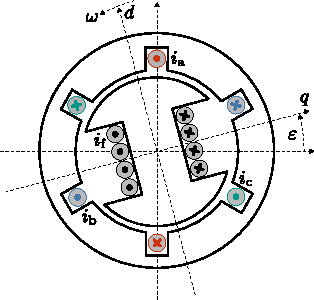
\includegraphics[width=0.8\textwidth]{fig/lec03/SM_salient_pole.pdf}
            \caption{Salient pole rotor}
        \end{subfigure}
        \hfill
        \begin{subfigure}{0.49\textwidth}
            \centering
            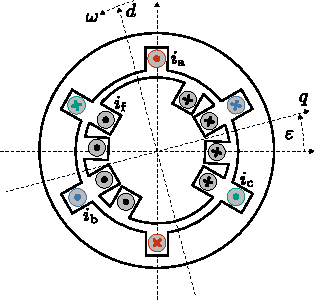
\includegraphics[width=0.8\textwidth]{fig/lec03/SM_cylindrical_rotor.pdf}
            \caption{Cylindrical rotor}
        \end{subfigure}
        \caption{Major rotor types of electrically excited synchronous machines (EESM) with dq reference frame axes aligned to the rotor flux produced by the field winding}
        \label{fig:examples_EESM_rotor}
    \end{figure}
\end{frame}

%%%%%%%%%%%%%%%%%%%%%%%%%%%%%%%%%%%%%%%%%%%%%%%%%%%%%%%%%%%%%
%% Summary: Cylindrical SM model in dq coordinates   %%
%%%%%%%%%%%%%%%%%%%%%%%%%%%%%%%%%%%%%%%%%%%%%%%%%%%%%%%%%%%%%
\begin{frame}
    \frametitle{EESM model in dq coordinates}
    The most important equations of the EESM model in the  dq coordinates are\footnote{A detailed derivation can be found in \href{https://github.com/IAS-Uni-Siegen/EMD_course}{Fundamentals of electrical machines and drives (EMD) course}.}:
    \begin{alignat}{4}
         &  & \text{Stator voltage:} &  & \quad\bm{u}_\mathrm{s,dq}( & t) &  & = R_\mathrm{s} \bm{i}_\mathrm{s,dq}(t)+ \omega(t)\bm{J}\bm{\psi}_\mathrm{s,dq}(t) + \nicefrac{\mathrm{d}}{\mathrm{d}t}\bm{\psi}_\mathrm{s,dq}(t), \notag \\
        \onslide<2->{&  & \text{Rotor / field winding voltage:}      &  & \quad u_\mathrm{f}(            & t) &  & = R_\mathrm{f}i_\mathrm{f}(t)+\nicefrac{\mathrm{d}}{\mathrm{d}t}\psi_\mathrm{f}(t), \notag}                          \\
        \onslide<3->{&  & \text{Stator flux linkage:}                &  & \quad \bm{\psi}_\mathrm{s,dq}( & t) &  & =  \bm{f}_{\psi_\mathrm{s}}(\bm{i}_\mathrm{s,dq}(t), \psi_\mathrm{f}(t)), \label{eq:basic_EESM_model_set}}           \\
        \onslide<4->{&  & \text{Rotor / field winding flux linkage:} &  & \psi_\mathrm{f}(               & t) &  & =  \bm{f}_{\psi_\mathrm{f}}(i_{\mathrm{f}}(t), \bm{i}_\mathrm{s,dq}(t)), \notag}                                     \\
        \onslide<5->{&  & \text{Torque:}                             &  & \quad T(                       & t) &  & = \nicefrac{3}{2} p (\bm{i}_\mathrm{s,dq}(t))\T\bm{J}\bm{\psi}_\mathrm{s,dq}(t) \notag}
    \end{alignat}
    \onslide<6->{with the further signals and parameters:
            \begin{equation*}
                \begin{aligned}
                    \bm{i}_\mathrm{s,dq}: \text{stator current},                                                              &
                    \qquad i_\mathrm{f}  : \text{rotor / field winding current},                                                                                                                                                      \\
                    R_\mathrm{s}:                                                          \text{stator winding resistances}, &
                    \qquad R_\mathrm{f} : \text{rotor / field winding resistance},                                                                                                                                                    \\
                    p                                           : \text{pole pair number},                                    &
                    \qquad \omega = p\omega_\mathrm{me}                   : \text{electrical angular velocity,}                                                                                                                       \\
                    \bm{J}: \text{90° rotation matrix, cf. \eqref{eq:J_rotation}},                                            & \qquad \bm{f}_{\psi_\mathrm{s}}, {f}_{\psi_\mathrm{f}} : \text{stator / rotor flux linkage function}.
                \end{aligned}
            \end{equation*}}
\end{frame}


%%%%%%%%%%%%%%%%%%%%%%%%%%%%%%%%%%%%%%%%%%%%%%%%%%%%%%%%%%%%%
%% EESM current-to-flux maps   %%
%%%%%%%%%%%%%%%%%%%%%%%%%%%%%%%%%%%%%%%%%%%%%%%%%%%%%%%%%%%%%
\begin{frame}
    \frametitle{EESM current-to-flux maps: nonlinear magnetic saturation}

    \begin{figure}
        \begin{tikzpicture}
            \begin{groupplot}[
                    group style={group size=3 by 1, horizontal sep=1.6cm},
                    width=0.32\textwidth,
                    height=0.33\textwidth,
                    view={-45}{24},
                    xlabel={$i_{\mathrm{d}}\,/\,\mathrm{A}$},
                    ylabel={$i_{\mathrm{q}}\,/\,\mathrm{A}$},
                    xmin=-30, xmax=10,
                    ymin=-35, ymax=35,
                    enlargelimits=false,
                    xtick={-30,-15,0,10},
                    ytick={-30,-15,0,15,30},
                    grid=major,
                    grid style={line width=.1pt, draw=gray!40},
                    tick label style={font=\small},
                    label style={font=\normalsize},
                    zlabel style={font=\normalsize},
                    title style={font=\normalsize},
                    xlabel style={yshift=2ex},
                    ylabel style={yshift=2ex},
                ]
                \nextgroupplot[
                    zlabel={$\psi_{\mathrm{d}}\,/\,\mathrm{Vs}$},
                    zmin=-0.50, zmax=1.05,
                ]
                \addplot3[surf, mesh/rows=15, mesh/cols=9, draw=black, shader=flat, fill=signaldelta, opacity=0.78] table[x=id_A,y=iq_A,z=psi_d_Vs_if2,col sep=comma] {fig/lec03/EESM_psi_d.csv};
                \addplot3[surf, mesh/rows=15, mesh/cols=9, draw=black, shader=flat, fill=signalgamma, opacity=0.74] table[x=id_A,y=iq_A,z=psi_d_Vs_if3,col sep=comma] {fig/lec03/EESM_psi_d.csv};
                \addplot3[surf, mesh/rows=15, mesh/cols=9, draw=black, shader=flat, fill=signalbeta, opacity=0.70] table[x=id_A,y=iq_A,z=psi_d_Vs_if4,col sep=comma] {fig/lec03/EESM_psi_d.csv};
                \addplot3[surf, mesh/rows=15, mesh/cols=9, draw=black, shader=flat, fill=signalalpha, opacity=0.66] table[x=id_A,y=iq_A,z=psi_d_Vs_if5,col sep=comma] {fig/lec03/EESM_psi_d.csv};

                \nextgroupplot[
                    zlabel={$\psi_{\mathrm{q}}\,/\,\mathrm{Vs}$},
                    zmin=-1.35, zmax=1.05,
                    zlabel style={yshift=-1ex},
                ]
                \addplot3[surf, mesh/rows=15, mesh/cols=9, draw=black, shader=flat, fill=signaldelta, opacity=0.78] table[x=id_A,y=iq_A,z=psi_q_Vs_if2,col sep=comma] {fig/lec03/EESM_psi_q.csv};
                \addplot3[surf, mesh/rows=15, mesh/cols=9, draw=black, shader=flat, fill=signalgamma, opacity=0.74] table[x=id_A,y=iq_A,z=psi_q_Vs_if3,col sep=comma] {fig/lec03/EESM_psi_q.csv};
                \addplot3[surf, mesh/rows=15, mesh/cols=9, draw=black, shader=flat, fill=signalbeta, opacity=0.70] table[x=id_A,y=iq_A,z=psi_q_Vs_if4,col sep=comma] {fig/lec03/EESM_psi_q.csv};
                \addplot3[surf, mesh/rows=15, mesh/cols=9, draw=black, shader=flat, fill=signalalpha, opacity=0.66] table[x=id_A,y=iq_A,z=psi_q_Vs_if5,col sep=comma] {fig/lec03/EESM_psi_q.csv};

                \nextgroupplot[
                    zlabel={$\psi_{\mathrm{f}}\,/\,\mathrm{Vs}$},
                    zmin=0.24, zmax=1.10,
                    zlabel style={yshift=-1ex},
                ]
                \addplot3[surf, mesh/rows=15, mesh/cols=9, draw=black, shader=flat, fill=signaldelta, opacity=0.78] table[x=id_A,y=iq_A,z=psi_f_Vs_if2,col sep=comma] {fig/lec03/EESM_psi_f.csv};
                \addplot3[surf, mesh/rows=15, mesh/cols=9, draw=black, shader=flat, fill=signalgamma, opacity=0.74] table[x=id_A,y=iq_A,z=psi_f_Vs_if3,col sep=comma] {fig/lec03/EESM_psi_f.csv};
                \addplot3[surf, mesh/rows=15, mesh/cols=9, draw=black, shader=flat, fill=signalbeta, opacity=0.70] table[x=id_A,y=iq_A,z=psi_f_Vs_if4,col sep=comma] {fig/lec03/EESM_psi_f.csv};
                \addplot3[surf, mesh/rows=15, mesh/cols=9, draw=black, shader=flat, fill=signalalpha, opacity=0.66] table[x=id_A,y=iq_A,z=psi_f_Vs_if5,col sep=comma] {fig/lec03/EESM_psi_f.csv};
            \end{groupplot}

            \matrix[matrix of nodes,
                ampersand replacement=\&,
                anchor=south,
                draw=black,
                fill=white,
                inner sep=1.4pt,
                row sep=1pt,
                column sep=5pt,
                nodes={anchor=west, font=\small}]
            at ($(group c1r1.north)!0.5!(group c3r1.north)+(0,0.5cm)$) {
                \tikz{\draw[draw=black, fill=signaldelta] (0,0) rectangle (0.40,0.16);} \& $i_{\mathrm{f}}=2\,\mathrm{A}$ \&
                \tikz{\draw[draw=black, fill=signalgamma] (0,0) rectangle (0.40,0.16);} \& $i_{\mathrm{f}}=3\,\mathrm{A}$ \&
                \tikz{\draw[draw=black, fill=signalbeta] (0,0) rectangle (0.40,0.16);} \& $i_{\mathrm{f}}=4\,\mathrm{A}$ \&
                \tikz{\draw[draw=black, fill=signalalpha] (0,0) rectangle (0.40,0.16);} \& $i_{\mathrm{f}}=5\,\mathrm{A}$ \\
            };
        \end{tikzpicture}
        \caption{Exemplary current-to-flux maps for a \SI{11}{\kilo\watt} EESM (derived from \href{https://www.mdpi.com/2079-9292/14/24/4924}{10.3390/electronics14244924}, \href{https://creativecommons.org/licenses/by/4.0/deed.en}{CC BY 4.0})}
        \label{fig:flux_maps_EESM}
    \end{figure}
\end{frame}

%%%%%%%%%%%%%%%%%%%%%%%%%%%%%%%%%%%%%%%%%%%%%%%%%%%%%%%%%%%%%
%% EESM differential inductance maps   %%
%%%%%%%%%%%%%%%%%%%%%%%%%%%%%%%%%%%%%%%%%%%%%%%%%%%%%%%%%%%%%
\begin{frame}
    \frametitle{EESM current-to-flux maps (cont.): differential inductances}
    \begin{figure}
        \begin{tikzpicture}
            \begin{groupplot}[
                    group style={group size=2 by 2, horizontal sep=2.55cm, vertical sep=0.6cm},
                    width=0.4\textwidth,
                    height=0.285\textwidth,
                    xlabel={$i_{\mathrm{d}}\,/\,\mathrm{A}$},
                    ylabel={$i_{\mathrm{q}}\,/\,\mathrm{A}$},
                    xmin=-30, xmax=10,
                    ymin=-35, ymax=35,
                    xtick={-30,-15,0,10},
                    ytick={-30,-15,0,15,30},
                    xlabel style={yshift=2ex},
                    ylabel style={yshift=2ex},
                    view={-45}{40},
                    enlargelimits=false,
                    grid=major,
                    grid style={line width=.1pt, draw=gray!40},
                    tick label style={font=\small},
                    label style={font=\small},
                    title style={font=\small},
                ]
                \nextgroupplot[
                    zlabel={$L_{\mathrm{dd}}\,/\,\mathrm{mH}$},
                    zmin=0, zmax=26,
                ]
                \addplot3[surf, mesh/rows=15, mesh/cols=9, shader=flat, draw=black, fill=signaldelta, opacity=0.78] table[x=id_A,y=iq_A,z=Ldd_mH_if2,col sep=comma] {fig/lec03/EESM_Ldd.csv};
                \addplot3[surf, mesh/rows=15, mesh/cols=9, shader=flat, draw=black, fill=signalgamma, opacity=0.74] table[x=id_A,y=iq_A,z=Ldd_mH_if3,col sep=comma] {fig/lec03/EESM_Ldd.csv};
                \addplot3[surf, mesh/rows=15, mesh/cols=9, shader=flat, draw=black, fill=signalbeta, opacity=0.70] table[x=id_A,y=iq_A,z=Ldd_mH_if4,col sep=comma] {fig/lec03/EESM_Ldd.csv};
                \addplot3[surf, mesh/rows=15, mesh/cols=9, shader=flat, draw=black, fill=signalalpha, opacity=0.66] table[x=id_A,y=iq_A,z=Ldd_mH_if5,col sep=comma] {fig/lec03/EESM_Ldd.csv};

                \nextgroupplot[
                    zlabel={$L_{\mathrm{dq}}\,/\,\mathrm{mH}$},
                    zmin=-3, zmax=10,
                ]
                \addplot3[surf, mesh/rows=15, mesh/cols=9, shader=flat, draw=black, fill=signaldelta, opacity=0.78] table[x=id_A,y=iq_A,z=Ldq_mH_if2,col sep=comma] {fig/lec03/EESM_Ldq.csv};
                \addplot3[surf, mesh/rows=15, mesh/cols=9, shader=flat, draw=black, fill=signalgamma, opacity=0.74] table[x=id_A,y=iq_A,z=Ldq_mH_if3,col sep=comma] {fig/lec03/EESM_Ldq.csv};
                \addplot3[surf, mesh/rows=15, mesh/cols=9, shader=flat, draw=black, fill=signalbeta, opacity=0.70] table[x=id_A,y=iq_A,z=Ldq_mH_if4,col sep=comma] {fig/lec03/EESM_Ldq.csv};
                \addplot3[surf, mesh/rows=15, mesh/cols=9, shader=flat, draw=black, fill=signalalpha, opacity=0.66] table[x=id_A,y=iq_A,z=Ldq_mH_if5,col sep=comma] {fig/lec03/EESM_Ldq.csv};

                \nextgroupplot[
                    zlabel={$L_{\mathrm{qd}}\,/\,\mathrm{mH}$},
                    zmin=-4, zmax=4,
                ]
                \addplot3[surf, mesh/rows=15, mesh/cols=9, shader=flat, draw=black, fill=signaldelta, opacity=0.78] table[x=id_A,y=iq_A,z=Lqd_mH_if2,col sep=comma] {fig/lec03/EESM_Lqd.csv};
                \addplot3[surf, mesh/rows=15, mesh/cols=9, shader=flat, draw=black, fill=signalgamma, opacity=0.74] table[x=id_A,y=iq_A,z=Lqd_mH_if3,col sep=comma] {fig/lec03/EESM_Lqd.csv};
                \addplot3[surf, mesh/rows=15, mesh/cols=9, shader=flat, draw=black, fill=signalbeta, opacity=0.70] table[x=id_A,y=iq_A,z=Lqd_mH_if4,col sep=comma] {fig/lec03/EESM_Lqd.csv};
                \addplot3[surf, mesh/rows=15, mesh/cols=9, shader=flat, draw=black, fill=signalalpha, opacity=0.66] table[x=id_A,y=iq_A,z=Lqd_mH_if5,col sep=comma] {fig/lec03/EESM_Lqd.csv};

                \nextgroupplot[
                    zlabel={$L_{\mathrm{qq}}\,/\,\mathrm{mH}$},
                    zmin=-25, zmax=55,
                ]
                \addplot3[surf, mesh/rows=15, mesh/cols=9, shader=flat, draw=black, fill=signaldelta, opacity=0.78] table[x=id_A,y=iq_A,z=Lqq_mH_if2,col sep=comma] {fig/lec03/EESM_Lqq.csv};
                \addplot3[surf, mesh/rows=15, mesh/cols=9, shader=flat, draw=black, fill=signalgamma, opacity=0.74] table[x=id_A,y=iq_A,z=Lqq_mH_if3,col sep=comma] {fig/lec03/EESM_Lqq.csv};
                \addplot3[surf, mesh/rows=15, mesh/cols=9, shader=flat, draw=black, fill=signalbeta, opacity=0.70] table[x=id_A,y=iq_A,z=Lqq_mH_if4,col sep=comma] {fig/lec03/EESM_Lqq.csv};
                \addplot3[surf, mesh/rows=15, mesh/cols=9, shader=flat, draw=black, fill=signalalpha, opacity=0.66] table[x=id_A,y=iq_A,z=Lqq_mH_if5,col sep=comma] {fig/lec03/EESM_Lqq.csv};
            \end{groupplot}

            % Legend    
            % \matrix[matrix of nodes,
            %     ampersand replacement=\&,
            %     anchor=west,
            %     draw=black,
            %     fill=white,
            %     inner sep=1.4pt,
            %     row sep=3pt,
            %     column sep=5pt,
            %     nodes={anchor=west, font=\small}]
            % at ($(group c2r1.east)!0.5!(group c2r2.east)+(0.5cm,0)$) {
            %     \tikz{\draw[draw=black, fill=signaldelta] (0,0) rectangle (0.40,0.16);} \& $i_{\mathrm{f}}=2\,\mathrm{A}$ \\
            %     \tikz{\draw[draw=black, fill=signalgamma] (0,0) rectangle (0.40,0.16);} \& $i_{\mathrm{f}}=3\,\mathrm{A}$ \\
            %     \tikz{\draw[draw=black, fill=signalbeta] (0,0) rectangle (0.40,0.16);} \& $i_{\mathrm{f}}=4\,\mathrm{A}$ \\
            %     \tikz{\draw[draw=black, fill=signalalpha] (0,0) rectangle (0.40,0.16);} \& $i_{\mathrm{f}}=5\,\mathrm{A}$ \\
            % };
        \end{tikzpicture}
        \caption{Exemplary differential inductance maps derived from \figref{fig:flux_maps_EESM}}
        \label{fig:inductance_maps_EESM}
    \end{figure}
\end{frame}

%%%%%%%%%%%%%%%%%%%%%%%%%%%%%%%%%%%%%%%%%%%%%%%%%%%%%%%%%%%%%
%% EESM differential inductance matrix %%
%%%%%%%%%%%%%%%%%%%%%%%%%%%%%%%%%%%%%%%%%%%%%%%%%%%%%%%%%%%%%
\begin{frame}
    \frametitle{EESM differential inductance matrix}
    Introducing the combined current and flux vectors for the EESM
    \begin{equation}
        \bm{i}_\mathrm{E}(t) = \begin{bmatrix} i_\mathrm{s,d}(t) & i_\mathrm{s,q}(t) & i_\mathrm{f}(t) \end{bmatrix}\T
        \quad  \text{and} \quad
        \bm{\psi}_\mathrm{E}(t) = \begin{bmatrix} \psi_\mathrm{s,d}(t) & \psi_\mathrm{s,q}(t) & \psi_\mathrm{f}(t) \end{bmatrix}\T,
    \end{equation}\pause
    its \hl{nonlinear magnetic model}\footnote{Extension towards rotor angle-dependent flux harmonics is analogous to PMSM and not explicitly shown here.} can be written compactly as
    \begin{equation}
        \bm{\psi}_\mathrm{E}(t) = \bm{f}_{\psi,\mathrm{E}}(\bm{i}_\mathrm{E}(t)).
    \end{equation}\pause
    Applying the chain rule yields the EESM differential inductance matrix
    \begin{equation}
        \frac{\mathrm{d}}{\mathrm{d}t}\bm{\psi}_\mathrm{E}(t) = \underbrace{\frac{\partial \bm{f}_{\psi,\mathrm{E}}}{\partial \bm{i}_\mathrm{E}}}_{\displaystyle=\,\bm{L}_\mathrm{E}(\bm{i}_\mathrm{E})} \frac{\mathrm{d}}{\mathrm{d}t}\bm{i}_\mathrm{E}(t)
        = \begin{bmatrix}
            L_{\mathrm{dd}}(\bm{i}_\mathrm{E}) & L_{\mathrm{dq}}(\bm{i}_\mathrm{E}) & L_{\mathrm{df}}(\bm{i}_\mathrm{E}) \\
            L_{\mathrm{qd}}(\bm{i}_\mathrm{E}) & L_{\mathrm{qq}}(\bm{i}_\mathrm{E}) & L_{\mathrm{qf}}(\bm{i}_\mathrm{E}) \\
            L_{\mathrm{fd}}(\bm{i}_\mathrm{E}) & L_{\mathrm{fq}}(\bm{i}_\mathrm{E}) & L_{\mathrm{ff}}(\bm{i}_\mathrm{E})
        \end{bmatrix} \frac{\mathrm{d}}{\mathrm{d}t}\bm{i}_\mathrm{E}(t).
    \end{equation}
\end{frame}

%%%%%%%%%%%%%%%%%%%%%%%%%%%%%%%%%%%%%%%%%%%%%%%%%%%%%%%%%%%%%
%% EESM current ODE %%
%%%%%%%%%%%%%%%%%%%%%%%%%%%%%%%%%%%%%%%%%%%%%%%%%%%%%%%%%%%%%
\begin{frame}
    \frametitle{Current differential equations of the nonlinear EESM model}
    With the compact voltage equation
    \begin{equation}
        \bm{u}_\mathrm{E}(t) = \bm{R}_\mathrm{E}\bm{i}_\mathrm{E}(t) + \bm{\Omega}(\omega)\bm{\psi}_\mathrm{E}(t) + \frac{\mathrm{d}}{\mathrm{d}t}\bm{\psi}_\mathrm{E}(t),
    \end{equation}
    and
    \begin{equation}
        \bm{u}_\mathrm{E} = \begin{bmatrix} \bm{u}_\mathrm{s,dq} \\ u_\mathrm{f} \end{bmatrix},
        \quad
        \bm{R}_\mathrm{E} = \operatorname{diag}(R_\mathrm{s}, R_\mathrm{s}, R_\mathrm{f}),
        \quad
        \bm{\Omega}(\omega) = \begin{bmatrix}
            \omega\bm{J}       & \bm{0}_{2\times 1} \\
            \bm{0}_{1\times 2} & 0
        \end{bmatrix},
    \end{equation}\pause
    substitution of $\frac{\mathrm{d}}{\mathrm{d}t}\bm{\psi}_\mathrm{E} = \bm{L}_\mathrm{E}(\bm{i}_\mathrm{E})\frac{\mathrm{d}}{\mathrm{d}t}\bm{i}_\mathrm{E}$ gives the \hl{EESM's nonlinear current ODE}
    \begin{equation}
        \frac{\mathrm{d}}{\mathrm{d}t}\bm{i}_\mathrm{E}(t) = \bm{L}_\mathrm{E}^{-1}(\bm{i}_\mathrm{E})\left[\bm{u}_\mathrm{E}(t) - \bm{R}_\mathrm{E}\bm{i}_\mathrm{E}(t) - \bm{\Omega}(\omega)\bm{f}_{\psi,\mathrm{E}}(\bm{i}_\mathrm{E}(t))\right].
    \end{equation}\pause
    In this nonlinear case, the torque expression remains
    \begin{equation}
        T(t) = \nicefrac{3}{2} p (\bm{i}_\mathrm{s,dq}(t))\T\bm{J}\bm{\psi}_\mathrm{s,dq}(t).
    \end{equation}
\end{frame}

%%%%%%%%%%%%%%%%%%%%%%%%%%%%%%%%%%%%%%%%%%%%%%%%%%%%%%%%%%%%%
%% Linear EESM model %%
%%%%%%%%%%%%%%%%%%%%%%%%%%%%%%%%%%%%%%%%%%%%%%%%%%%%%%%%%%%%%
\begin{frame}
    \frametitle{Linear EESM model with constant inductances}
    Around some operating point, a compact linear magnetic model is obtained as
    \begin{equation}
        \bm{\psi}_\mathrm{E}(t) \approx \bm{L}_{\mathrm{E},0}\bm{i}_\mathrm{E}(t),
        \qquad
        \bm{L}_{\mathrm{E},0} = \begin{bmatrix}
            L_{\mathrm{dd},0} & 0                 & L_{\mathrm{df},0} \\
            0                 & L_{\mathrm{qq},0} & 0                 \\
            L_{\mathrm{fd},0} & 0                 & L_{\mathrm{ff},0}
        \end{bmatrix},
    \end{equation}
    where the weak cross-couplings $L_{\mathrm{dq},0}$, $L_{\mathrm{qd},0}$, $L_{\mathrm{qf},0}$ and $L_{\mathrm{fq},0}$ are neglected. \pause
    The corresponding \hl{linear EESM current} ODE becomes
    \begin{equation}
        \frac{\mathrm{d}}{\mathrm{d}t}\bm{i}_\mathrm{E}(t) = \bm{L}_{\mathrm{E},0}^{-1}\left[\bm{u}_\mathrm{E}(t) - \bm{R}_\mathrm{E}\bm{i}_\mathrm{E}(t) - \bm{\Omega}(\omega)\bm{L}_{\mathrm{E},0}\bm{i}_\mathrm{E}(t)\right].
    \end{equation}\pause
    For this simplified linear magnetic model, the torque expression simplifies to
    \begin{equation}
        T(t) = \frac{3}{2}p\left[L_{\mathrm{df},0} i_\mathrm{f}(t)i_\mathrm{s,q}(t) + (L_{\mathrm{dd},0}-L_{\mathrm{qq},0})i_\mathrm{s,d}(t)i_\mathrm{s,q}(t)\right].
    \end{equation}
\end{frame}


%%%%%%%%%%%%%%%%%%%%%%%%%%%%%%%%%%%%%%%%%%%%%%%%%%%%%%%%%%%%%%%%%%
\subsection{Discrete-time machine models}
%%%%%%%%%%%%%%%%%%%%%%%%%%%%%%%%%%%%%%%%%%%%%%%%%%%%%%%%%%%%%%%%%%

%%%%%%%%%%%%%%%%%%%%%%%%%%%%%%%%%%%%%%%%%%%%%%%%%%%%%%%%%%%%%
%% RK1 discrete-time model of the nonlinear PMSM model %%
%%%%%%%%%%%%%%%%%%%%%%%%%%%%%%%%%%%%%%%%%%%%%%%%%%%%%%%%%%%%%
\begin{frame}
    \frametitle{RK1 discrete-time model of the nonlinear PMSM model}
    Based on the nonlinear flux ODE PMSM \eqref{eq:basic_PMSM_model_set}
    \begin{equation*}
        \frac{\mathrm{d}}{\mathrm{d}t}\bm{\psi}_\mathrm{s,dq}(t)  = \bm{u}_\mathrm{s,dq}(t) - R_\mathrm{s} \bm{i}_\mathrm{s,dq}(t)- \omega(t)\bm{J}\bm{\psi}_\mathrm{s,dq}(t)
    \end{equation*}\pause
    applying the \hl{explicit Euler method (RK1)} from \eqref{eq:RK1} yields the discrete-time model
    \begin{equation}
        \bm{\psi}_\mathrm{s,dq}[k+1] = \bm{\psi}_\mathrm{s,dq}[k] + T_\mathrm{s}\left(\bm{u}_\mathrm{s,dq}[k] - R_\mathrm{s} \bm{i}_\mathrm{s,dq}[k]- \omega[k]\bm{J}\bm{\psi}_\mathrm{s,dq}[k]\right),
    \end{equation}
    where $T_\mathrm{s}$ is the sampling period and $k$ is the \hl{discrete time index}. \pause Likewise, the \hl{implicit Euler method (IRK1)} from \eqref{eq:IRK1} gives
    \begin{equation}
        \begin{split}
            \bm{\psi}_\mathrm{s,dq}[k+1]                 & = \bm{\psi}_\mathrm{s,dq}[k] + T_\mathrm{s}\left(\bm{u}_\mathrm{s,dq}[k+1] - R_\mathrm{s} \bm{i}_\mathrm{s,dq}[k+1]- \omega[k+1]\bm{J}\bm{\psi}_\mathrm{s,dq}[k+1]\right)                        \\
            \Leftrightarrow \bm{\psi}_\mathrm{s,dq}[k+1] & = \left(\bm{I} + T_\mathrm{s}\omega[k+1]\bm{J}\right)^{-1}\left(\bm{\psi}_\mathrm{s,dq}[k] + T_\mathrm{s}\left(\bm{u}_\mathrm{s,dq}[k+1] - R_\mathrm{s} \bm{i}_\mathrm{s,dq}[k+1]\right)\right).
        \end{split}
        \label{eq:IRK1_nonlinear_flux_ODE_PMSM}
    \end{equation}
\end{frame}


%%%%%%%%%%%%%%%%%%%%%%%%%%%%%%%%%%%%%%%%%%%%%%%%%%%%%%%%%%%%%
%% RK1 discrete-time model of the nonlinear PMSM model (con.t) %%
%%%%%%%%%%%%%%%%%%%%%%%%%%%%%%%%%%%%%%%%%%%%%%%%%%%%%%%%%%%%%
\begin{frame}
    \frametitle{RK1 discrete-time model of the nonlinear PMSM model (cont.)}
    Since  the first-order RK methods are known to be inaccurate, we analyze the \hl{induced voltage terms} of the RK1 and IRK1 discrete-time models:
    \begin{equation}
        \text{RK1:} \, \bm{u}_\mathrm{ind.} = -\omega[k]\bm{J}\bm{\psi}_\mathrm{s,dq}[k] \quad \text{vs.} \quad \text{IRK1:} \, \bm{u}_\mathrm{ind.} = -\omega[k+1]\bm{J}\bm{\psi}_\mathrm{s,dq}[k+1].
        \label{eq:induc_voltages_RK1_IRK1_nonlinear_flux_ODE_PMSM}
    \end{equation}\pause
    Considering the $\nicefrac{\pi}{2}$ rotation of $\bm{J}$ from \eqref{eq:J_rotation}, we can directly conclude that the induced voltage is orthogonal to the flux linkage vector at time $k$:
    \begin{equation*}
        \text{RK1:} \, \angle\left(\bm{u}_\mathrm{ind.}, \bm{\psi}_\mathrm{s,dq}[k]\right) = \frac{\pi}{2}.
    \end{equation*}\pause
    For the IRK1 method, we first need to express $\bm{\psi}_\mathrm{s,dq}[k+1]$ in terms of $\bm{\psi}_\mathrm{s,dq}[k]$: neglecting the input and ohmic voltage terms in \eqref{eq:IRK1_nonlinear_flux_ODE_PMSM} gives
    $$
        \bm{\psi}_\mathrm{s,dq}[k+1] \approx \left(\bm{I} + T_\mathrm{s}\omega[k+1]\bm{J}\right)^{-1}\bm{\psi}_\mathrm{s,dq}[k] = \frac{1}{1+(T_\mathrm{s}\omega[k+1])^2}\left(\bm{I} - T_\mathrm{s}\omega[k+1]\bm{J}\right)\bm{\psi}_\mathrm{s,dq}[k].
    $$
\end{frame}

%%%%%%%%%%%%%%%%%%%%%%%%%%%%%%%%%%%%%%%%%%%%%%%%%%%%%%%%%%%%%
%% RK1 discrete-time model of the nonlinear PMSM model (con.t) %%
%%%%%%%%%%%%%%%%%%%%%%%%%%%%%%%%%%%%%%%%%%%%%%%%%%%%%%%%%%%%%
\begin{frame}
    \frametitle{RK1 discrete-time model of the nonlinear PMSM model (cont.)}
    Substituting this approximation into the IRK1 induced voltage term from \eqref{eq:induc_voltages_RK1_IRK1_nonlinear_flux_ODE_PMSM} yields
    \begin{equation*}
        \begin{split}
            \bm{u}_\mathrm{ind.} & = -\omega[k+1]\bm{J}\bm{\psi}_\mathrm{s,dq}[k+1] \\ &\approx -\frac{\omega[k+1]}{1+(T_\mathrm{s}\omega[k+1])^2}(\underbrace{\bm{J}\bm{\psi}_{\mathrm{s,dq}}[k]}_{\text{orthogonal to } \bm{\psi}_\mathrm{s,dq}[k]} - \underbrace{T_\mathrm{s}\omega[k+1]\bm{I}\bm{\psi}_\mathrm{s,dq}[k]}_{\text{parallel to} \bm{\psi}_\mathrm{s,dq}[k]} ).
        \end{split}
    \end{equation*}\pause
    Hence, the IRK1 induced voltage vector relative to the flux vector $\bm{\psi}_\mathrm{s,dq}[k]$ is given by
    \begin{equation*}
        \text{IRK1:} \, \angle\left(\bm{u}_\mathrm{ind.}, \bm{\psi}_\mathrm{s,dq}[k]\right) = \arctan\left(\frac{1}{T_\mathrm{s}\omega[k+1]}\right) = \frac{\pi}{2} - \arctan\left(T_\mathrm{s}\omega[k+1]\right).
    \end{equation*}\pause
    Consequently, for any $\omega[k+1]>0$, the IRK1 induced voltage vector is less than $\nicefrac{\pi}{2}$ shifted towards the flux vector.
\end{frame}

%%%%%%%%%%%%%%%%%%%%%%%%%%%%%%%%%%%%%%%%%%%%%%%%%%%%%%%%%%%%%
%% RK1 discrete-time model of the nonlinear PMSM model (con.t) %%
%%%%%%%%%%%%%%%%%%%%%%%%%%%%%%%%%%%%%%%%%%%%%%%%%%%%%%%%%%%%%
\begin{frame}
    \frametitle{RK1 discrete-time model of the nonlinear PMSM model (cont.)}
    \begin{figure}
        \centering
        \begin{tikzpicture}[scale=0.93, >=Latex, line cap=round, line join=round]
            % fixed axes
            \draw[black, line width=0.9pt, -{Latex[length=3.2mm,width=2.2mm]}] (0,0) -- (5.0,0) node[below right=-1pt] {$\alpha$};
            \draw[black, line width=0.9pt, -{Latex[length=3.2mm,width=2.2mm]}] (0,-0.45) -- (0,5) node[above left=-1pt] {$\beta$};

            % dq axes for the beginning of the step
            \draw[black, line width=0.8pt, -{Latex[length=2.8mm,width=2.0mm]}] (0,0) -- (15:5) node[right=-1pt] {$d$};
            \draw[black, line width=0.8pt, -{Latex[length=2.8mm,width=2.0mm]}] (0,0) -- (105:5) node[above left=-1pt] {$q$};

            % only the relevant circular arc between the alpha-axis and the larger angle
            \draw[black, dashed, line width=0.8pt] (3.55,0) arc[start angle=0,end angle=180,radius=3.55];

            % flux vectors
            \coordinate (Psik) at (70:3.553);
            \coordinate (Psikp) at (42:3.553);
            \draw[signalalpha, line width=1.0pt, -{Latex[length=3.0mm,width=2.1mm]}] (0,0) -- (Psik);
            \draw[signalalpha, line width=1.0pt, -{Latex[length=3.0mm,width=2.1mm]}] (0,0) -- (Psikp);
            \fill[black] (Psik) circle (1.6pt);
            \fill[black] (Psikp) circle (1.6pt);

            % induced voltages
            \draw[signaldelta, dashed, line width=1.0pt, -{Latex[length=3.0mm,width=2.1mm]}]
            (Psik) -- ++(70-90:1.5);
            \draw[signaldelta, dashed, line width=1.0pt, -{Latex[length=3.0mm,width=2.1mm]}]
            (Psik) -- ++(42-90:1.5);
            \draw[signaldelta, dashed, line width=1.0pt, -{Latex[length=3.0mm,width=2.1mm]}]
            (Psikp) -- ++(42-90:1.5);


            % labels
            \node[above, signalalpha] at (Psik) {$\bm{\psi}_{\mathrm{dq}}[k]$};
            \node[right, signalalpha] at (Psikp) {$\bm{\psi}_{\mathrm{dq}}[k{+}1]$};

            \node[above right, signaldelta] at (55:3.6) {$-\omega_{\mathrm{rs}}[k]\,\bm{J}\bm{\psi}_{\mathrm{dq}}[k]$ (RK1)};
            \node[right, signaldelta] at (27:3.75) {$-\omega_{\mathrm{rs}}[k{+}1]\,\bm{J}\bm{\psi}_{\mathrm{dq}}[k{+}1]$ (IRK1)};
        \end{tikzpicture}
        \caption{Impact of the time discretization on the induced voltage interpretation: in the explicit RK1 case, the induced voltage vector tends to increase the flux vector length in the next time step (excess virtual energy; lack of damping), while in the implicit IRK1 case, the induced voltage vector tends to decrease the flux vector length in the next time step (virtual energy dissipation; added damping).}
        \label{fig:rk1_irk1_induced_voltage_angle_dependency}
    \end{figure}
\end{frame}

%%%%%%%%%%%%%%%%%%%%%%%%%%%%%%%%%%%%%%%%%%%%%%%%%%%%%%%%%%%%%
%% Alternative discretization path: discretize in $\upalpha\upbeta$-frame first  %%
%%%%%%%%%%%%%%%%%%%%%%%%%%%%%%%%%%%%%%%%%%%%%%%%%%%%%%%%%%%%%
\begin{frame}
    \frametitle{Alternative discretization path: discretize in $\upalpha\upbeta$-frame first}
    Instead of the $\mathrm{dq}$ model \eqref{eq:basic_PMSM_model_set}, we can also start from the \hl{$\upalpha\upbeta$ flux linkage ODE}\footnote{Compare derivation again: \href{https://github.com/IAS-Uni-Siegen/EMD_course}{Fundamentals of electrical machines and drives (EMD) course}.}:
    \begin{equation}
        \frac{\mathrm{d}}{\mathrm{d}t}\bm{\psi}_{\upalpha\upbeta}(t) = \bm{u}_{\upalpha\upbeta}(t) - R_\mathrm{s}\,\bm{i}_{\upalpha\upbeta}(t).
        \label{eq:PMSM_flux_ODE_alpha_beta}
    \end{equation}\pause
    The \hl{explicit RK1 discretization} of this ODE is given by
    \begin{equation}
        \bm{\psi}_{\upalpha\upbeta}[k+1] = \bm{\psi}_{\upalpha\upbeta}[k] + T_\mathrm{s}\left(\bm{u}_{\upalpha\upbeta}[k] - R_\mathrm{s}\,\bm{i}_{\upalpha\upbeta}[k]\right).
    \end{equation}\pause
    Applying the Park transformation \eqref{eq:Park_transformation} to both sides yields
    \begin{equation}
        \bm{T}_\mathrm{p}(\varepsilon[k+1])\bm{\psi}_{\mathrm{dq}}[k+1] = \bm{T}_\mathrm{p}(\varepsilon[k])\left(\bm{\psi}_\mathrm{dq}[k] + T_\mathrm{s}\left(\bm{u}_\mathrm{dq}[k] - R_\mathrm{s}\,\bm{i}_\mathrm{dq}[k]\right)\right).
    \end{equation}\pause
    Assuming a nearly constant rotor speed $\omega[k]=\omega[k+1]$ during two sampling steps
    $$
        \bm{T}^{-1}_\mathrm{p}(\varepsilon[k+1])\bm{T}_\mathrm{p}(\varepsilon[k])=\bm{T}_\mathrm{p}(-\varepsilon[k+1])\bm{T}_\mathrm{p}(\varepsilon[k]) = \bm{T}_\mathrm{p}(\varepsilon[k]-\varepsilon[k+1]) = \bm{T}_\mathrm{p}(-\omega[k]T_\mathrm{s}),
    $$\pause
    we can rewrite the above equation as
    \begin{equation}
        \bm{\psi}_{\mathrm{dq}}[k+1] = \bm{T}_\mathrm{p}(-\omega[k]T_\mathrm{s})\left(\bm{\psi}_{\mathrm{dq}}[k] + T_\mathrm{s}\left(\bm{u}_{\mathrm{dq}}[k] - R_\mathrm{s}\,\bm{i}_{\mathrm{dq}}[k]\right)\right).
    \end{equation}
\end{frame}

%%%%%%%%%%%%%%%%%%%%%%%%%%%%%%%%%%%%%%%%%%%%%%%%%%%%%%%%%%%%%
%% Alternative discretization path: discretize in $\upalpha\upbeta$-frame first (cont.) %%
%%%%%%%%%%%%%%%%%%%%%%%%%%%%%%%%%%%%%%%%%%%%%%%%%%%%%%%%%%%%%
\begin{frame}
    \frametitle{Alternative discretization path: discretize in $\upalpha\upbeta$-frame first (cont.)}
    Mildly rearranging the above equation yields for the \hl{RK1 case}
    \begin{equation}
        \bm{\psi}_{\mathrm{dq}}[k+1] = \bm{\psi}_{\mathrm{dq}}[k] - \left(\bm{I} -\bm{T}_\mathrm{p}(-\omega[k]T_\mathrm{s})\right)\bm{\psi}_{\mathrm{dq}}[k]+\bm{T}_\mathrm{p}(-\omega[k]T_\mathrm{s})T_\mathrm{s}\left(\bm{u}_{\mathrm{dq}}[k] - R_\mathrm{s}\,\bm{i}_{\mathrm{dq}}[k]\right).
    \end{equation}\pause
    Applying the \hl{analogous steps for the IRK1} case starting from \eqref{eq:PMSM_flux_ODE_alpha_beta} yields
    \begin{equation}
        \bm{\psi}_{\mathrm{dq}}[k+1] = \bm{\psi}_{\mathrm{dq}}[k] - \left(\bm{I} -\bm{T}_\mathrm{p}(-\omega[k+1]T_\mathrm{s})\right)\bm{\psi}_{\mathrm{dq}}[k]+T_\mathrm{s}\left(\bm{u}_{\mathrm{dq}}[k+1] - R_\mathrm{s}\,\bm{i}_{\mathrm{dq}}[k+1]\right).
    \end{equation}\pause
    Following again the assumption $\omega[k]=\omega[k+1]$, we can identify that the induced voltage terms are identical for both discretization paths:
    \begin{equation*}
        \bm{u}_\mathrm{ind.}=T_\mathrm{s}\left(\bm{I} -\bm{T}_\mathrm{p}(-\omega[k]T_\mathrm{s})\right)\bm{\psi}_{\mathrm{dq}}[k] = T_\mathrm{s}\left(\bm{I} -\bm{T}_\mathrm{p}(-\omega[k+1]T_\mathrm{s})\right)\bm{\psi}_{\mathrm{dq}}[k].
    \end{equation*}\pause
    Not considering the input and ohmic voltage impacts, this term can be interpreted as the \hl{flux change in between two sampling steps}:
    \begin{equation}
        \frac{\bm{\psi}_{\mathrm{dq}}[k+1] - \bm{\psi}_{\mathrm{dq}}[k]}{T_\mathrm{s}}=\left(\bm{I} -\bm{T}_\mathrm{p}(-\omega[k]T_\mathrm{s})\right)\bm{\psi}_{\mathrm{dq}}[k]=\left(\bm{I} -\bm{T}_\mathrm{p}(-\omega[k+1]T_\mathrm{s})\right)\bm{\psi}_{\mathrm{dq}}[k].
    \end{equation}
\end{frame}

%%%%%%%%%%%%%%%%%%%%%%%%%%%%%%%%%%%%%%%%%%%%%%%%%%%%%%%%%%%%%
%% Alternative discretization path: discretize in $\upalpha\upbeta$-frame first (cont.) %%
%%%%%%%%%%%%%%%%%%%%%%%%%%%%%%%%%%%%%%%%%%%%%%%%%%%%%%%%%%%%%
\begin{frame}
    \frametitle{Alternative discretization path: discretize in $\upalpha\upbeta$-frame first (cont.)}
    \begin{figure}
        \centering
        \begin{tikzpicture}[scale=0.93, >=Latex, line cap=round, line join=round]
            % fixed axes
            \draw[black, line width=0.9pt, -{Latex[length=3.2mm,width=2.2mm]}] (0,0) -- (5.0,0) node[below right=-1pt] {$\alpha$};
            \draw[black, line width=0.9pt, -{Latex[length=3.2mm,width=2.2mm]}] (0,-0.45) -- (0,5) node[above left=-1pt] {$\beta$};

            % dq axes for the beginning of the step
            \draw[black, line width=0.8pt, -{Latex[length=2.8mm,width=2.0mm]}] (0,0) -- (15:5) node[right=-1pt] {$d$};
            \draw[black, line width=0.8pt, -{Latex[length=2.8mm,width=2.0mm]}] (0,0) -- (105:5) node[above left=-1pt] {$q$};

            % only the relevant circular arc between the alpha-axis and the larger angle
            \draw[black, dashed, line width=0.8pt] (3.55,0) arc[start angle=0,end angle=180,radius=3.55];

            % flux vectors
            \coordinate (Psik) at (70:3.553);
            \coordinate (Psikp) at (42:3.553);
            \draw[signalalpha, line width=1.0pt, -{Latex[length=3.0mm,width=2.1mm]}] (0,0) -- (Psik);
            \draw[signalalpha, line width=1.0pt, -{Latex[length=3.0mm,width=2.1mm]}] (0,0) -- (Psikp);
            \fill[black] (Psik) circle (1.6pt);
            \fill[black] (Psikp) circle (1.6pt);

            % induced voltages
            \draw[signaldelta, dashed, line width=1.0pt, -{Latex[length=3.0mm,width=2.1mm]}]
            (Psik) -- (Psikp);



            % labels
            \node[above, signalalpha] at (Psik) {$\bm{\psi}_{\mathrm{dq}}[k]$};
            \node[right, signalalpha] at (Psikp) {$\bm{\psi}_{\mathrm{dq}}[k{+}1]$};

            \node[above right, signaldelta] at (55:3.6) {$\left(\bm{I} -\bm{T}_\mathrm{p}(-\omega[k]T_\mathrm{s})\right)\bm{\psi}_{\mathrm{dq}}[k]$};

        \end{tikzpicture}
        \caption{Interpretation of the induced voltage vector as the flux change in between two sampling steps when: \hl{discretize in $\upalpha\upbeta$-frame first, then utilize the Park transformation}. }
        \label{fig:rk1_irk1_induced_voltage_angle_dependency}
    \end{figure}
\end{frame}

%%%%%%%%%%%%%%%%%%%%%%%%%%%%%%%%%%%%%%%%%%%%%%%%%%%%%%%%%%%%%
%% Alternative discretization path: discretize in $\upalpha\upbeta$-frame first (cont.) %%
%%%%%%%%%%%%%%%%%%%%%%%%%%%%%%%%%%%%%%%%%%%%%%%%%%%%%%%%%%%%%
\begin{frame}
    \frametitle{Alternative discretization path: discretize in $\upalpha\upbeta$-frame first (cont.)}
    Since the IRK1 model is unhandy for control-related implementations due to the implicit nature, we consider the \hl{explicit RK1 model as a simple standard model} (discretized from the $\upalpha\upbeta$-frame):
    \begin{equation}
        \begin{alignedat}{4}
             &  & \mbox{Difference eq.:} &  & \quad\bm{\psi}_{\mathrm{dq}}[&k+1] &  & = \bm{T}_\mathrm{p}(-\omega[k]T_\mathrm{s})\left(\bm{\psi}_{\mathrm{dq}}[k] + T_\mathrm{s}\left(\bm{u}_{\mathrm{dq}}[k] - R_\mathrm{s}\,\bm{i}_{\mathrm{dq}}[k]\right)\right), \\
            \onslide<2->{&  & \mbox{Stator flux linkage:} &  & \quad \bm{\psi}_\mathrm{s,dq}[ & k+1] &  & = \bm{f}_{\psi_\mathrm{s}}(\bm{i}_\mathrm{s,dq}[k+1], \psi_\mathrm{PM}),}                                                                                  \\\onslide<3->{
                                                                                                                                                                                                                                                                                          &  & \mbox{Torque:}              &  & \quad T[                       & k+1] &  & = \nicefrac{3}{2} p (\bm{i}_\mathrm{s,dq}[k+1])\T\bm{J}\bm{\psi}_\mathrm{s,dq}[k+1].}
        \end{alignedat}
        \label{eq:basic_PMSM_model_set_RK1}
    \end{equation}
    \onslide<4->{A few remarks on the above model set:}
    \begin{itemize}
        \item<4-> Although typically more accurate and numerical robust than a direct RK1 discretization of the $\mathrm{dq}$-frame model, the above RK1 model is still an approximation of the continuous-time dynamics.
        \item<5-> Consequently, numerical errors cannot be completely avoided. The severity of the numerical errors depend on the specific machine parameters, operating point and sampling time.
        \item<6-> If interested in the stator currents, one can solve \eqref{eq:basic_PMSM_model_set_RK1} and then apply the inverse flux linkage map $\bm{f}_{\psi_\mathrm{s}}^{-1}(\cdot)$.
    \end{itemize}
\end{frame}

%%%%%%%%%%%%%%%%%%%%%%%%%%%%%%%%%%%%%%%%%%%%%%%%%%%%%%%%%%%%%
%% Current difference equation of the RK1 discrete-time model %%
%%%%%%%%%%%%%%%%%%%%%%%%%%%%%%%%%%%%%%%%%%%%%%%%%%%%%%%%%%%%%
\begin{frame}
    \frametitle{Current difference equation of the RK1 discrete-time model}

\end{frame} % Basic control of synchronous machines

%%%%%%%%%%%%%%%%%%%%%%%%%%%%%%%%%%%%%%%%%%%%%%%%%%%%%%%%%%%%%%%%%%
\section{Induction machine drives -- basic models and control concepts}
%%%%%%%%%%%%%%%%%%%%%%%%%%%%%%%%%%%%%%%%%%%%%%%%%%%%%%%%%%%%%%%%%%

%%%%%%%%%%%%%%%%%%%%%%%%%%%%%%%%%%%%%%%%%%%%%%%%%%%%%%%%%%%%%%%%%%
\subsection{Induction machine model}
%%%%%%%%%%%%%%%%%%%%%%%%%%%%%%%%%%%%%%%%%%%%%%%%%%%%%%%%%%%%%%%%%%

%%%%%%%%%%%%%%%%%%%%%%%%%%%%%%%%%%%%%%%%%%%%%%%%%%%%%%%%%%%%%
%% Basic induction machine (IM) representation %%
%%%%%%%%%%%%%%%%%%%%%%%%%%%%%%%%%%%%%%%%%%%%%%%%%%%%%%%%%%%%%
\begin{frame}[b]
	\frametitle{Basic induction machine (IM) representation}
	\begin{columns}
		\begin{column}{0.55\textwidth}
			\begin{itemize}
				\item Three-phase stator + three-phase rotor
				\item Rotor electrical angular speed: $\omega$
				\item Rotor electrical angular displacement: $\varepsilon$
				\item Index \enquote{s} for stator, \enquote{r} for rotor quantities
			\end{itemize}
			\begin{figure}
				\centering
				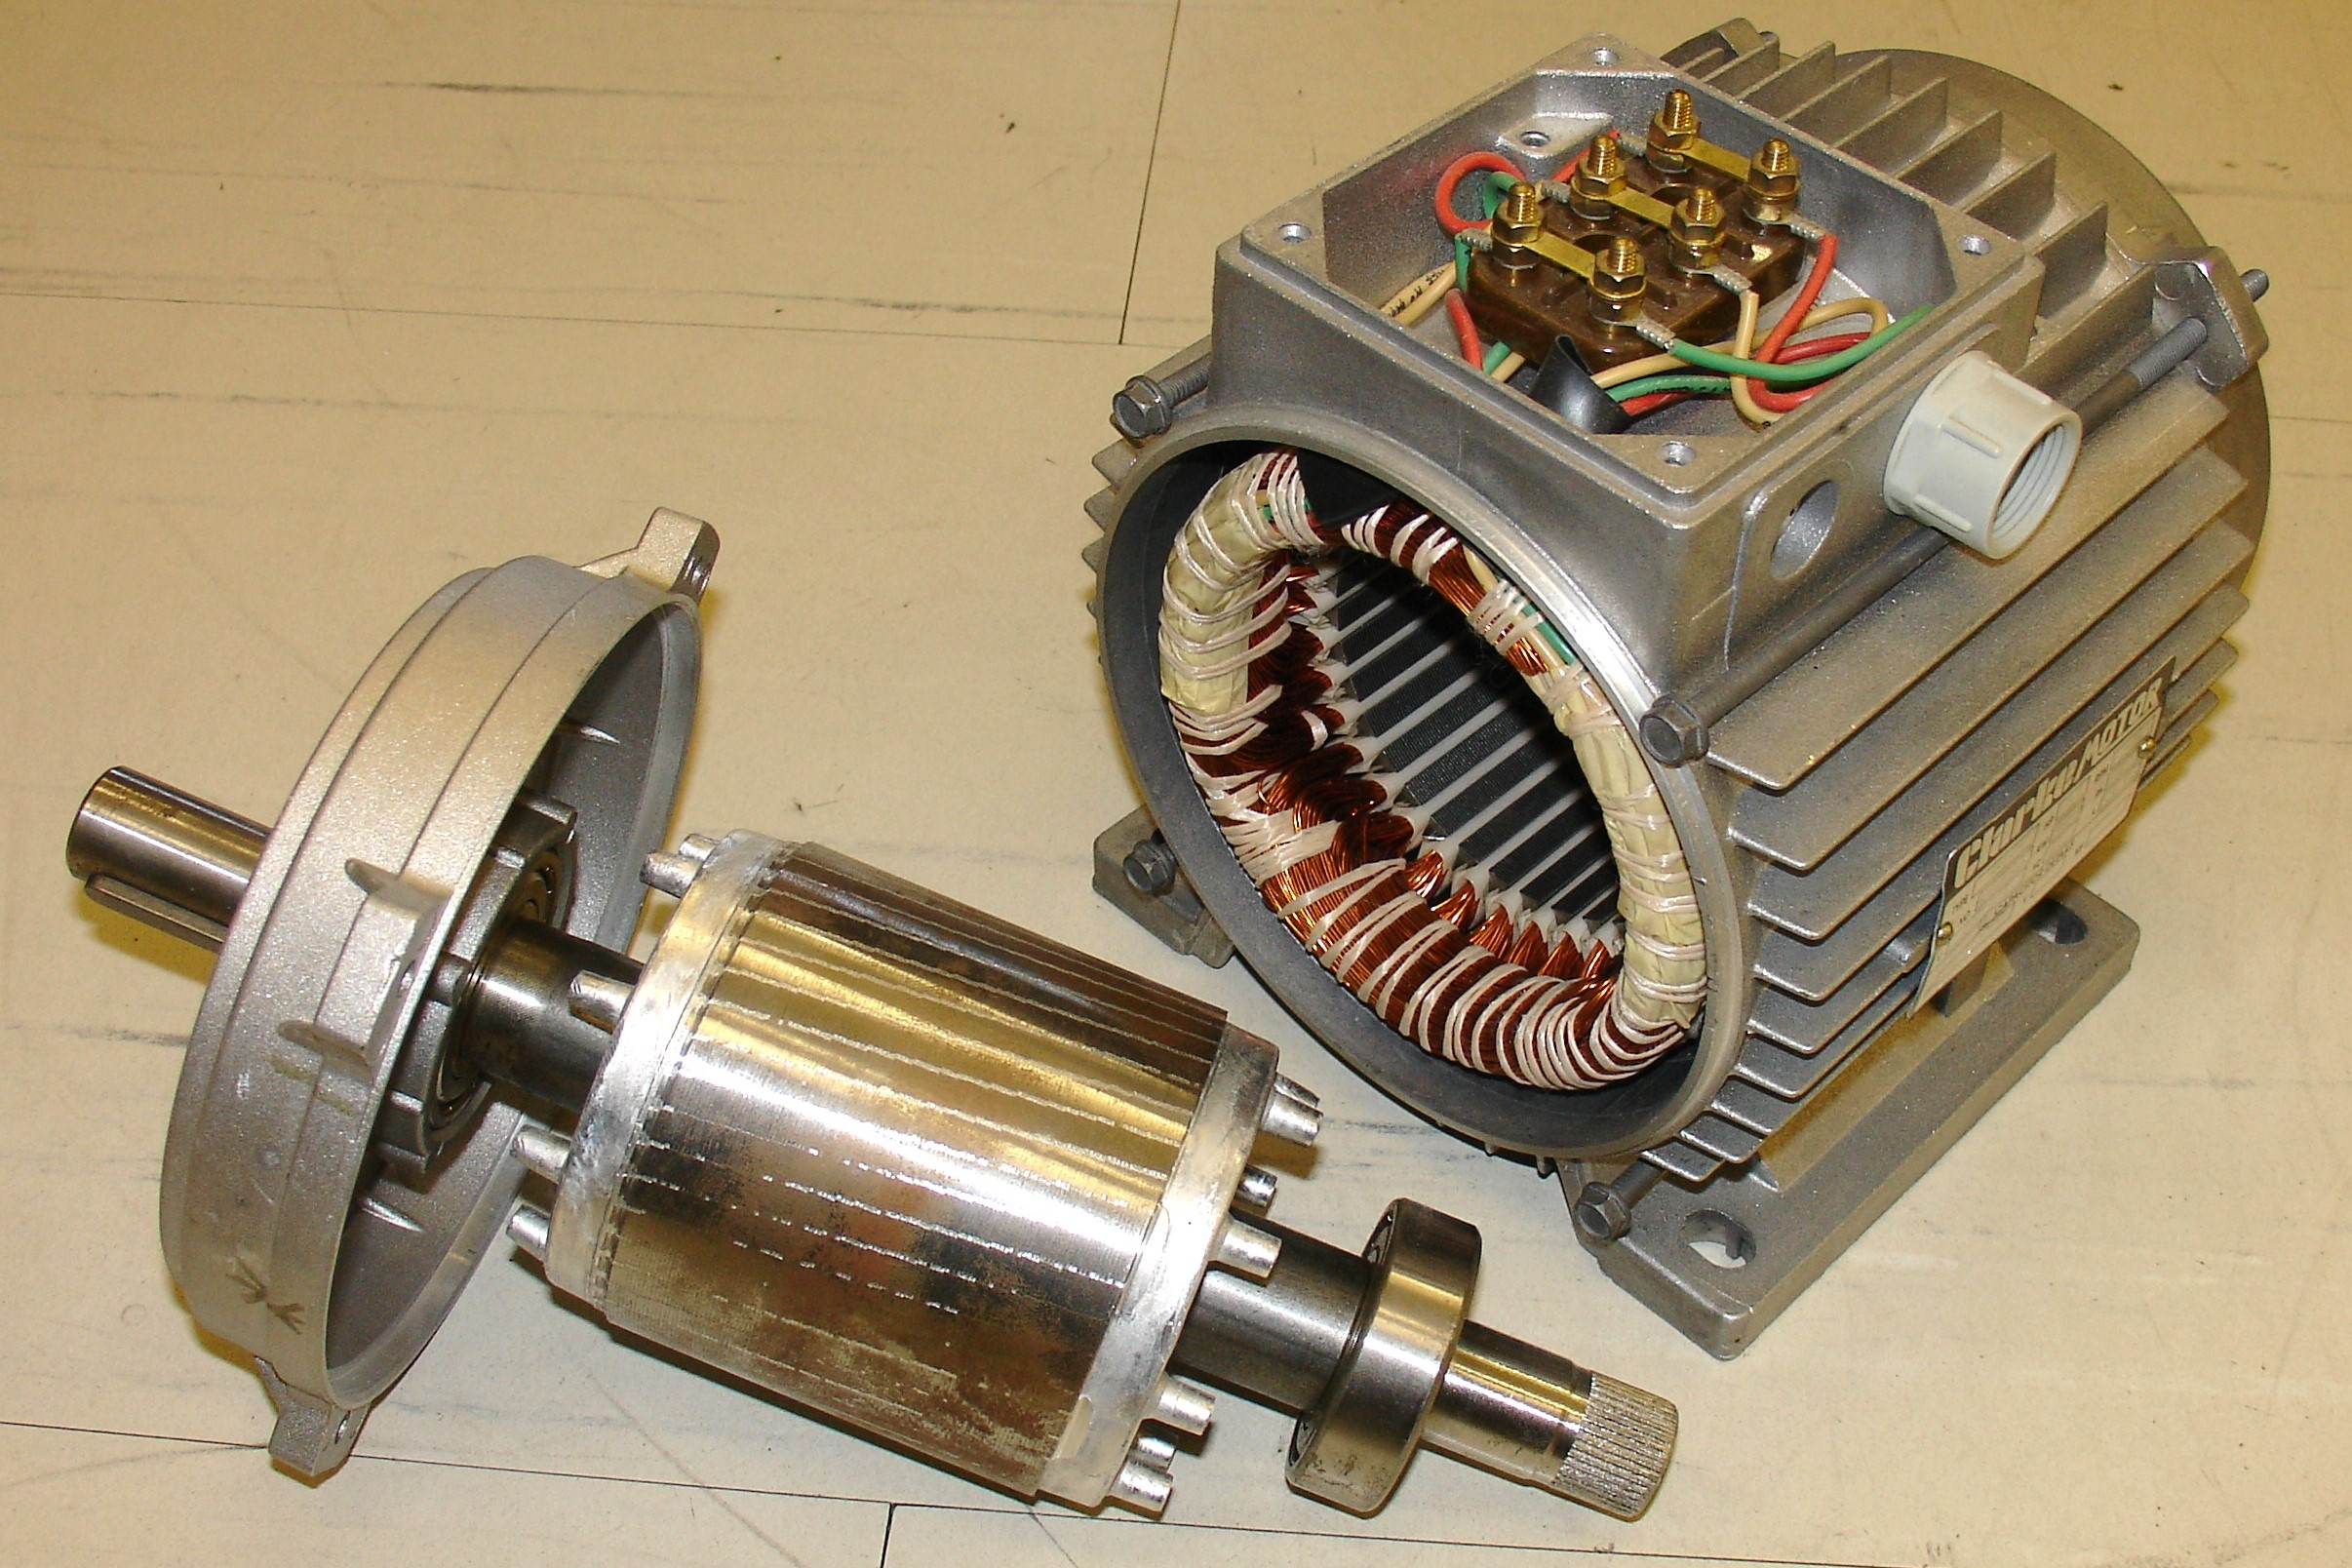
\includegraphics[width=0.525\textwidth]{fig/lec04/Induction_motor_stator_rotor.JPG}
				\caption{Induction machine with squirrel cage rotor (source: \href{https://commons.wikimedia.org/wiki/File:Stator_and_rotor_by_Zureks.JPG}{Wikimedia Commons}, Zureks, \href{https://creativecommons.org/licenses/by-sa/4.0/deed.en}{CC BY-SA 4.0})}
			\end{figure}
		\end{column}
		\begin{column}{0.45\textwidth}
			\begin{figure}
				\centering
				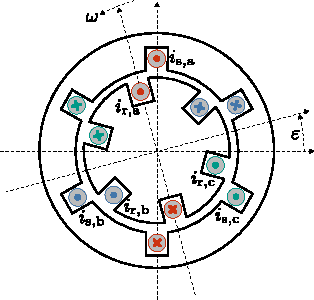
\includegraphics[width=0.85\textwidth]{fig/lec04/Simple_three_phase_induction_machine_lumped_coils.pdf}
				\caption{Elementary three-phase induction machine (IM)  with $p=1$ pole pair}
				\label{fig:Simple_three_phase_induction_machine_lumped_coils}
			\end{figure}
		\end{column}
	\end{columns}
\end{frame}

%%%%%%%%%%%%%%%%%%%%%%%%%%%%%%%%%%%%%%%%%%%%%%%%%%%%%%%%%%%%%
%% Summary: PMSM model in dq coordinates   %%
%%%%%%%%%%%%%%%%%%%%%%%%%%%%%%%%%%%%%%%%%%%%%%%%%%%%%%%%%%%%%
\begin{frame}
	\frametitle{IM model in dq coordinates}
	The most important equations of the squirrel cage IM model in the  dq coordinates with arbitrary orientation axis $\mathrm{k}$ (indicated as an upper index) are\footnote{A detailed derivation can be found in \href{https://github.com/IAS-Uni-Siegen/EMD_course}{Fundamentals of electrical machines and drives (EMD) course}. All quantities are already assumed to be transformed to the stator side (without further nomenclature hints).}:
	\begin{equation}
		\begin{alignedat}{4}
			\uncover<+->{ &  & \mbox{Stator voltage:}      &  & \quad\bm{u}^\mathrm{k}_\mathrm{s,dq}(     & t) &  & = R_\mathrm{s} \bm{i}^\mathrm{k}_\mathrm{s,dq}(t)+ \omega_\mathrm{k}(t)\bm{J}\bm{\psi}^\mathrm{k}_\mathrm{s,dq}(t) + \nicefrac{\mathrm{d}}{\mathrm{d}t}\bm{\psi}^\mathrm{k}_\mathrm{s,dq}(t),\\}
			\uncover<+->{ &  & \mbox{Rotor voltage:}       &  & & 0 &  & = R_\mathrm{r} \bm{i}^\mathrm{k}_\mathrm{r,dq}(t)+\left(\omega_\mathrm{k}(t)-\omega(t)\right)\bm{J}\bm{\psi}^\mathrm{k}_\mathrm{r,dq}(t) + \nicefrac{\mathrm{d}}{\mathrm{d}t}\bm{\psi}^\mathrm{k}_\mathrm{r,dq}(t),\\}
			\uncover<+->{&  & \mbox{Stator flux linkage:} &  & \quad \bm{\psi}^\mathrm{k}_\mathrm{s,dq}( & t) &  & = \bm{f}^\mathrm{k}_{\psi_\mathrm{s}}(\bm{i}^\mathrm{k}_\mathrm{s,dq}(t), \bm{i}^\mathrm{k}_\mathrm{r,dq}(t)),} \\
			\uncover<+->{&  & \mbox{Rotor flux linkage:} &  & \quad \bm{\psi}^\mathrm{k}_\mathrm{r,dq}( & t) &  & = \bm{f}^\mathrm{k}_{\psi_\mathrm{r}}(\bm{i}^\mathrm{k}_\mathrm{s,dq}(t), \bm{i}^\mathrm{k}_\mathrm{r,dq}(t)),}  \\\uncover<+->{
					                                                                                                                                                                                                                                    &  & \mbox{Torque:}              &  & \quad T(                       & t) &  & = \nicefrac{3}{2} p (\bm{i}^\mathrm{k}_\mathrm{s,dq}(t))\T\bm{J}\bm{\psi}^\mathrm{k}_\mathrm{s,dq}(t) = -\nicefrac{3}{2} p (\bm{i}^\mathrm{k}_\mathrm{r,dq}(t))\T\bm{J}\bm{\psi}^\mathrm{k}_\mathrm{r,dq}(t).}
		\end{alignedat}
		\label{eq:basic_IM_model_set}
	\end{equation}
	\onslide<6->{with the further new signals and parameters:
			\begin{equation*}
				\begin{aligned}
					 & \omega_\mathrm{k}: \text{(electrical) angular frequency of ref. axis $\mathrm{k}$},                                                        &  &
					\qquad \bm{\psi}^\mathrm{k}_\mathrm{s,dq}, \bm{\psi}^\mathrm{k}_\mathrm{r,dq}  : \text{nonlinear flux linkages},                                                                                                                                                   \\
					 & \omega_\mathrm{slip} =\omega_\mathrm{k} - \omega:                                                          \text{ slip angular frequency}. &  & \qquad R_\mathrm{r}:                                                          \text{rotor winding resistances}. \\
				\end{aligned}
			\end{equation*}}
\end{frame}

%%%%%%%%%%%%%%%%%%%%%%%%%%%%%%%%%%%%%%%%%%%%%%%%%%%%%%%%%%%%%
%% Stator flux orientation in the k coordinate system %%
%%%%%%%%%%%%%%%%%%%%%%%%%%%%%%%%%%%%%%%%%%%%%%%%%%%%%%%%%%%%%
\begin{frame}
	\frametitle{Stator flux linkage orientation}
	\begin{columns}
		\begin{column}{0.5\textwidth}
			Per definition we can assign the stator flux linkage to the $\mathrm{d}$-axis of the $\mathrm{k}$ coordinate system:
			\begin{equation}
				\renewcommand{\arraystretch}{1.4}
				\begin{split}
					\bm{\psi}^{\psi_{\mathrm{s}}}_\mathrm{s,dq}(t) & = \begin{bmatrix} \psi_{\mathrm{s,d}}^{\psi_{\mathrm{s}}}(t) \\ \psi_{\mathrm{s,q}}^{\psi_{\mathrm{s}}}(t) \end{bmatrix} = \begin{bmatrix} \psi_{\mathrm{s,d}}^{\psi_{\mathrm{s}}}(t) \\ 0 \end{bmatrix} \\
					                                               & = \begin{bmatrix}|\bm{\psi}^{\psi_{\mathrm{s}}}_\mathrm{s,dq}(t)| \\ 0 \end{bmatrix}.
				\end{split}
				\label{eq:IM_model_k_stator_flux_orientation_def}
			\end{equation}
			\onslide<2->{
					In this case, the torque expression simplifies to
					\begin{equation}
						T^{\psi_{\mathrm{s}}}(t)  = \frac{3}{2} p i_{\mathrm{s,q}}^{\psi_{\mathrm{s}}}(t)\psi_{\mathrm{s,d}}^{\psi_{\mathrm{s}}}(t) .
						\label{eq:IM_model_k_torque_stator_flux_orientation}
					\end{equation}
				}
		\end{column}
		\begin{column}{0.5\textwidth}
			\begin{figure}
				\centering
				\begin{tikzpicture}[>=Latex]

					% origin
					\coordinate (O) at (0,0);

					% stationary alpha-beta axes
					\draw[->] (-3.3,0) -- (3.35,0) node[right] {$\upalpha$};
					\draw[->] (0,-1.65) -- (0,3.95) node[right] {$\upbeta$};

					% rotating d-q axes
					\draw[thick] (O) -- ++(-35:1.7);
					\draw[thick, ->] (O) -- ++(145:3.05) node[below] {$\mathrm{q}$};

					\draw[thick] (O) -- ++(235:1.7);
					\draw[thick, ->] (O) -- ++(55:3.35) node[below right] {$\mathrm{d}$};

					% vectors
					\draw[signaldelta, ->, thick] (O) -- ++(105:2.88)
					node[pos=0.72, left=1mm] {$\bm{i}_{\mathrm{s,dq}}$};

					\draw[signalalpha,->, thick] (O) -- ++(55:2.75)
					node[pos=0.72, right=1mm] {$\bm{\psi}_{\mathrm{s,dq}}$};

					\draw[signalalpha,->, thick] (O) -- ++(23:2.45)
					node[pos=0.90, below right] {$\bm{\psi}_{\mathrm{r,dq}}$};

					% electrical angular velocity indication
					\draw[->, thin] (0,0) ++(45:3.6) arc (45:65:3.6) node[pos=0.5, above right] {$\omega_{\mathrm{k}}$};

				\end{tikzpicture}
				\caption{Stator flux-oriented coordinate system}
				\label{fig:K_coordinates_stator_flux_orientation}
			\end{figure}
		\end{column}
	\end{columns}
\end{frame}

%%%%%%%%%%%%%%%%%%%%%%%%%%%%%%%%%%%%%%%%%%%%%%%%%%%%%%%%%%%%%
%% Stator flux orientation in the k coordinate system %%
%%%%%%%%%%%%%%%%%%%%%%%%%%%%%%%%%%%%%%%%%%%%%%%%%%%%%%%%%%%%%
\begin{frame}
	\frametitle{Stator flux linkage orientation (cont.)}
	Rearranging the stator voltage equation towards a stator flux linkage differential equation yields
	\begin{equation}
		\begin{split}
			\frac{\mathrm{d}}{\mathrm{d}t}\bm{\psi}^{\psi_{\mathrm{s}}}_\mathrm{s,dq}(t)                                                               & = \bm{u}^{\psi_{\mathrm{s}}}_\mathrm{s,dq}(t) - R_\mathrm{s} \bm{i}^{\psi_{\mathrm{s}}}_\mathrm{s,dq}(t) - \omega_{\psi_{\mathrm{s}}}(t)\bm{J}\bm{\psi}^{\psi_{\mathrm{s}}}_\mathrm{s,dq}(t)                                                                                                                                                                                          \\ \Leftrightarrow \quad
			\frac{\mathrm{d}}{\mathrm{d}t}\begin{bmatrix} \psi^{\psi_{\mathrm{s}}}_\mathrm{s,d} \\ \psi^{\psi_{\mathrm{s}}}_\mathrm{s,q} \end{bmatrix} & = \begin{bmatrix} u_{\mathrm{s,d}}^{\psi_{\mathrm{s}}}(t) - R_\mathrm{s} i_{\mathrm{s,d}}^{\psi_{\mathrm{s}}}(t) + \omega_{\psi_{\mathrm{s}}}(t)\psi_{\mathrm{s,q}}^{\psi_{\mathrm{s}}}(t) \\ u_{\mathrm{s,q}}^{\psi_{\mathrm{s}}}(t) - R_\mathrm{s} i_{\mathrm{s,q}}^{\psi_{\mathrm{s}}}(t) - \omega_{\psi_{\mathrm{s}}}(t)\psi_{\mathrm{s,d}}^{\psi_{\mathrm{s}}}(t) \end{bmatrix}.
		\end{split}
		\label{eq:IM_model_k_stator_flux_orientation_differential_equation}
	\end{equation}\pause%
	Based on the orientation definition \eqref{eq:IM_model_k_stator_flux_orientation_def}, the $\mathrm{q}$-axis stator flux linkage differential component must be always zero, which implies
	\begin{equation}
		\frac{\mathrm{d}}{\mathrm{d}t}\psi_{\mathrm{s,q}}^{\psi_{\mathrm{s}}}(t) = 0 = u_{\mathrm{s,q}}^{\psi_{\mathrm{s}}}(t) - R_\mathrm{s} i_{\mathrm{s,q}}^{\psi_{\mathrm{s}}}(t) - \omega_{\psi_{\mathrm{s}}}(t)\psi_{\mathrm{s,d}}^{\psi_{\mathrm{s}}}(t).
	\end{equation}\pause%
	Hence, the \hl{stator flux angle} required for the reference frame of stator flux orientation is
	\begin{equation}
		\omega_{\psi_{\mathrm{s}}}(t) = \frac{1}{\psi_{\mathrm{s,d}}^{\psi_{\mathrm{s}}}(t)}\left(u_{\mathrm{s,q}}^{\psi_{\mathrm{s}}}(t) - R_\mathrm{s} i_{\mathrm{s,q}}^{\psi_{\mathrm{s}}}(t)\right) \quad \rightarrow \quad \varepsilon_{\psi_{\mathrm{s}}}(t) = \int_0^t \omega_{\psi_{\mathrm{s}}}(\tau) \mathrm{d}\tau.
		\label{eq:IM_model_k_stator_flux_orientation_angular_velocity}
	\end{equation}
\end{frame}

%%%%%%%%%%%%%%%%%%%%%%%%%%%%%%%%%%%%%%%%%%%%%%%%%%%%%%%%%%%%%
%% Stator flux orientation in the k coordinate system %%
%%%%%%%%%%%%%%%%%%%%%%%%%%%%%%%%%%%%%%%%%%%%%%%%%%%%%%%%%%%%%
\begin{frame}
	\frametitle{Rotor flux linkage orientation}
	\begin{columns}
		\begin{column}{0.5\textwidth}
			Alternatively, we can assign the rotor flux linkage to the $\mathrm{d}$-axis of the $\mathrm{k}$ coordinate system:
			\begin{equation}
				\renewcommand{\arraystretch}{1.4}
				\begin{split}
					\bm{\psi}^{\psi_{\mathrm{r}}}_\mathrm{r,dq}(t) & = \begin{bmatrix} \psi_{\mathrm{r,d}}^{\psi_{\mathrm{r}}}(t) \\ \psi_{\mathrm{r,q}}^{\psi_{\mathrm{r}}}(t) \end{bmatrix} = \begin{bmatrix} \psi_{\mathrm{r,d}}^{\psi_{\mathrm{r}}}(t) \\ 0 \end{bmatrix} \\
					                                               & = \begin{bmatrix}|\bm{\psi}^{\psi_{\mathrm{r}}}_\mathrm{r,dq}(t)| \\ 0 \end{bmatrix}.
				\end{split}
				\label{eq:IM_model_k_rotor_flux_orientation_def}
			\end{equation}
			\onslide<2->{
					In this case, the torque expression simplifies to
					\begin{equation}
						T^{\psi_{\mathrm{r}}}(t)  = -\frac{3}{2} p i_{\mathrm{r,q}}^{\psi_{\mathrm{r}}}(t)\psi_{\mathrm{r,d}}^{\psi_{\mathrm{r}}}(t) .
						\label{eq:IM_model_k_torque_rotor_flux_orientation}
					\end{equation}
				}
		\end{column}
		\begin{column}{0.5\textwidth}
			\begin{figure}
				\centering
				\begin{tikzpicture}[>=Latex]

					% origin
					\coordinate (O) at (0,0);

					% stationary alpha-beta axes
					\draw[->] (-3.3,0) -- (3.35,0) node[right] {$\upalpha$};
					\draw[->] (0,-1.65) -- (0,3.95) node[right] {$\upbeta$};

					% rotating d-q axes
					\draw[thick] (O) -- ++(293:1.7);
					\draw[thick, ->] (O) -- ++(113:3.05) node[left] {$\mathrm{q}$};

					\draw[thick] (O) -- ++(203:1.7);
					\draw[thick, ->] (O) -- ++(23:3.35) node[below] {$\mathrm{d}$};

					% vectors
					\draw[signaldelta, ->, thick] (O) -- ++(105:2.88)
					node[above] {$\bm{i}_{\mathrm{s,dq}}$};

					\draw[signalalpha,->, thick] (O) -- ++(55:2.75)
					node[pos=0.72, right=1mm] {$\bm{\psi}_{\mathrm{s,dq}}$};

					\draw[signalalpha,->, thick] (O) -- ++(23:2.45)
					node[pos=0.90, below right] {$\bm{\psi}_{\mathrm{r,dq}}$};

					% electrical angular velocity indication
					\draw[->, thin] (0,0) ++(13:3.6) arc (13:33:3.6) node[pos=0.5, above right] {$\omega_{\mathrm{k}}$};

				\end{tikzpicture}
				\caption{Rotor flux-oriented coordinate system}
				\label{fig:K_coordinates_rotor_flux_orientation}
			\end{figure}
		\end{column}
	\end{columns}
\end{frame}

%%%%%%%%%%%%%%%%%%%%%%%%%%%%%%%%%%%%%%%%%%%%%%%%%%%%%%%%%%%%%
%% Stator flux orientation in the k coordinate system %%
%%%%%%%%%%%%%%%%%%%%%%%%%%%%%%%%%%%%%%%%%%%%%%%%%%%%%%%%%%%%%
\begin{frame}
	\frametitle{Rotor flux linkage orientation (cont.)}
	Rearranging the rotor voltage equation towards a rotor flux linkage differential equation yields
	\begin{equation}
		\begin{split}
			\frac{\mathrm{d}}{\mathrm{d}t}\bm{\psi}^{\psi_{\mathrm{r}}}_\mathrm{r,dq}(t)                                                                                    & = - R_\mathrm{r} \bm{i}^{\psi_{\mathrm{r}}}_\mathrm{r,dq}(t) - \left(\omega_{\psi_{\mathrm{r}}}(t)-\omega(t)\right)\bm{J}\bm{\psi}^{\psi_{\mathrm{r}}}_\mathrm{r,dq}(t)                                                                                                                                                                             \\
			\Leftrightarrow \quad\frac{\mathrm{d}}{\mathrm{d}t}\begin{bmatrix} \psi^{\psi_{\mathrm{r}}}_\mathrm{r,d} \\ \psi^{\psi_{\mathrm{r}}}_\mathrm{r,q} \end{bmatrix} & = \begin{bmatrix} - R_\mathrm{r} i_{\mathrm{r,d}}^{\psi_{\mathrm{r}}}(t) + \left(\omega_{\psi_{\mathrm{r}}}(t)-\omega(t)\right)\psi_{\mathrm{r,q}}^{\psi_{\mathrm{r}}}(t) \\ - R_\mathrm{r} i_{\mathrm{r,q}}^{\psi_{\mathrm{r}}}(t) - \left(\omega_{\psi_{\mathrm{r}}}(t)-\omega(t)\right)\psi_{\mathrm{r,d}}^{\psi_{\mathrm{r}}}(t) \end{bmatrix}.
		\end{split}
		\label{eq:IM_model_k_rotor_flux_orientation_differential_equation}
	\end{equation}\pause%
	Based on the orientation definition \eqref{eq:IM_model_k_rotor_flux_orientation_def}, the $\mathrm{q}$-axis rotor flux linkage differential component must be always zero, which implies
	\begin{equation}
		\frac{\mathrm{d}}{\mathrm{d}t}\psi_{\mathrm{r,q}}^{\psi_{\mathrm{r}}}(t) = 0 = - R_\mathrm{r} i_{\mathrm{r,q}}^{\psi_{\mathrm{r}}}(t) - \left(\omega_{\psi_{\mathrm{r}}}(t)-\omega(t)\right)\psi_{\mathrm{r,d}}^{\psi_{\mathrm{r}}}(t).
	\end{equation}\pause%
	Hence, the \hl{rotor flux angle} required for the reference frame of rotor flux orientation is
	\begin{equation}
		\omega_{\psi_{\mathrm{r}}}(t) = \omega(t) - \frac{1}{\psi_{\mathrm{r,d}}^{\psi_{\mathrm{r}}}(t)} R_\mathrm{r} i_{\mathrm{r,q}}^{\psi_{\mathrm{r}}}(t) \quad \rightarrow \quad \varepsilon_{\psi_{\mathrm{r}}}(t) = \int_0^t \omega_{\psi_{\mathrm{r}}}(\tau) \mathrm{d}\tau.
		\label{eq:IM_model_k_rotor_flux_orientation_angular_velocity}
	\end{equation}\pause%
	Here, the term $\omega_\mathrm{slip} = -\nicefrac{R_\mathrm{r} i_{\mathrm{r,q}}^{\psi_{\mathrm{r}}}}{\psi_{\mathrm{r,d}}^{\psi_{\mathrm{r}}}} $ is the \hl{slip angular frequency}, i.e., the difference between the rotor flux angular velocity and the rotor speed (impacting the rotor's induced voltage).
\end{frame}

%%%%%%%%%%%%%%%%%%%%%%%%%%%%%%%%%%%%%%%%%%%%%%%%%%%%%%%%%%%%%
\subsubsection{Nonlinear parameter submodels}
%%%%%%%%%%%%%%%%%%%%%%%%%%%%%%%%%%%%%%%%%%%%%%%%%%%%%%%%%%%%%

%%%%%%%%%%%%%%%%%%%%%%%%%%%%%%%%%%%%%%%%%%%%%%%%%%%%%%%%%%%%%
%% Slip frequency-dependent rotor skin effect%%
%%%%%%%%%%%%%%%%%%%%%%%%%%%%%%%%%%%%%%%%%%%%%%%%%%%%%%%%%%%%%
\begin{frame}
	\frametitle{Slip frequency-dependent rotor skin effect}
	\begin{columns}
		\begin{column}{0.55\textwidth}
			\begin{itemize}
				\item<1-> If $\omega_\mathrm{slip} \neq 0$, the rotor bars are exposed to a time-varying magnetic field.
				\item<2-> This induces eddy currents leading to an uneven current distribution within the bars.
				\item<3-> As a result, the effective rotor resistance increases with the slip frequency: \begin{equation}
					      \frac{R_\mathrm{r}(\omega_\mathrm{slip})}{R_\mathrm{r,DC}} =  \delta \frac{\sinh(2 \delta) + \sin(2 \delta)}{\cosh(2\delta)-\cos(2 \delta)}
				      \end{equation}
				      with $$\delta = h_\mathrm{bar}\sqrt{|\omega_\mathrm{slip}| \frac{\mu_0 \kappa}{2}\frac{w_\mathrm{bar}}{w_\mathrm{slot}}}.$$ Here, $\mu_0$ is the vacuum permeability and $\kappa$ is the bar's conductivity.
			\end{itemize}
		\end{column}
		\begin{column}{0.45\textwidth}
			\onslide<1->
			\begin{figure}
				\centering
				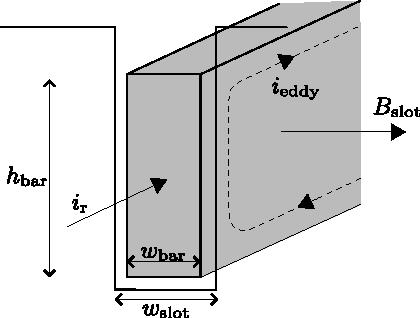
\includegraphics[width=0.85\textwidth]{fig/lec04/Eddy_currents_rotor_bar.pdf}
				\caption{Rotor bar with eddy currents induced by the rotating magnetic field (inspired from A. Binder, \textit{Elektrische Maschinen und Antriebe}, Vol. 2, Springer, 2017)}
				\label{fig:Eddy_currents_rotor_bar}
			\end{figure}
		\end{column}
	\end{columns}
\end{frame}

%%%%%%%%%%%%%%%%%%%%%%%%%%%%%%%%%%%%%%%%%%%%%%%%%%%%%%%%%%%%%
%% Slip frequency-dependent rotor skin effect (cont.)%%
%%%%%%%%%%%%%%%%%%%%%%%%%%%%%%%%%%%%%%%%%%%%%%%%%%%%%%%%%%%%%
% ------------------------------------------------------------
% Rotor skin-effect resistance ratio
% ------------------------------------------------------------
% Parameters:
% kappa  = 3.7e7 S/m
% hbar   = 50 mm
% wbar   = 10 mm
% wslot  = 15 mm
% mu0    = 4*pi*1e-7 H/m
%
% omega_slip = 2*pi*f_slip
% ------------------------------------------------------------

\pgfkeys{/pgf/fpu=true}
\pgfmathsetmacro{\SkinCoeff}{%
	50e-3*sqrt(2*pi*4*pi*1e-7*3.7e7/2*10e-3/15e-3)%
}
\pgfkeys{/pgf/fpu=false}

\pgfmathdeclarefunction{skinDelta}{1}{%
	\pgfmathparse{\SkinCoeff*sqrt(max(#1,1e-9))}%
}

\pgfmathdeclarefunction{skinRratio}{1}{%
	\pgfmathparse{%
		skinDelta(#1)
		*(sinh(2*skinDelta(#1)) + sin(deg(2*skinDelta(#1))))
		/(cosh(2*skinDelta(#1)) - cos(deg(2*skinDelta(#1))))%
	}%
}
\begin{frame}
	\frametitle{Slip frequency-dependent rotor skin effect (cont.)}
	\begin{figure}
		\centering
		\begin{tikzpicture}
			\begin{axis}[
					width=0.85\textwidth,
					height=0.65\textheight,
					xmin=0,
					xmax=50,
					ymin=1,
					ymax=3.5,
					xlabel={$f_{\mathrm{slip}}=\nicefrac{\omega_{\mathrm{slip}}}{2\pi}\ \mathrm{in\ Hz}$},
					ylabel={$\dfrac{R_{\mathrm r}(\omega_{\mathrm{slip}})}{R_{\mathrm{r,DC}}}$},
					xtick={0,10,20,30,40,50},
					ytick={1,1.5,2,2.5,3},
					grid=major,
				]
				\addplot[
					signalblue,
					thick,
					domain=0:50,
					samples=501,
					smooth
				] {skinRratio(x)};
			\end{axis}
		\end{tikzpicture}
		\caption{Rotor resistance of a squirrel cage IM as a function of the slip frequency (example based on the following values: $\kappa = \SI[per-mode=repeated-symbol, fraction-function=\nicefrac]{3.7\cdot10^7}{\siemens\per\metre}$, $h_\mathrm{bar} = \SI{50}{\milli\metre}$, $w_\mathrm{bar} = \SI{10}{\milli\metre}$, $w_\mathrm{slot} = \SI{15}{\milli\metre}$)}
		\label{fig:AC_rotor_resistance}
	\end{figure}
\end{frame}


%%%%%%%%%%%%%%%%%%%%%%%%%%%%%%%%%%%%%%%%%%%%%%%%%%%%%%%%%%%%%
%% Motivation %%
%%%%%%%%%%%%%%%%%%%%%%%%%%%%%%%%%%%%%%%%%%%%%%%%%%%%%%%%%%%%%
\begin{frame}
	\frametitle{Why an explicit IM flux linkage model?}
	The nonlinear squirrel cage IM model from \eqref{eq:IM_general_flux_functions} requires an explicit flux linkage model
	\begin{equation}
		\bm{\psi}^\mathrm{k}_\mathrm{s,dq}(t)=\bm{f}^\mathrm{k}_{\psi_\mathrm{s}}\big(\bm{i}^\mathrm{k}_\mathrm{s,dq}(t),\bm{i}^\mathrm{k}_\mathrm{r,dq}(t)\big), \quad
		\bm{\psi}^\mathrm{k}_\mathrm{r,dq}(t)=\bm{f}^\mathrm{k}_{\psi_\mathrm{r}}\big(\bm{i}^\mathrm{k}_\mathrm{s,dq}(t),\bm{i}^\mathrm{k}_\mathrm{r,dq}(t)\big).
		\label{eq:IM_general_flux_functions}
	\end{equation}
	\begin{itemize}
		\item<2-> For PMSMs, current-to-flux maps can be tabulated over the measurable stator currents.
		\item<3-> For squirrel cage IMs, the rotor currents are latent quantities and cannot be directly excited independently nor measured.
		\item<4-> Hence, a LUT in $(\bm{i}_\mathrm{s,dq},\bm{i}_\mathrm{r,dq})$ is not directly identifiable from steady-state stator voltage/current data.
		\item<5-> Instead, an explicit flux linkage model will be used as part of the overall IM model, which can be parameterized based on experimental data (covering both steady-state and transient conditions plus eventually further measurements such as torque).
	\end{itemize}
\end{frame}


%%%%%%%%%%%%%%%%%%%%%%%%%%%%%%%%%%%%%%%%%%%%%%%%%%%%%%%%%%%%%
%% Branch currents %%
%%%%%%%%%%%%%%%%%%%%%%%%%%%%%%%%%%%%%%%%%%%%%%%%%%%%%%%%%%%%%
\begin{frame}
	\frametitle{Current coordinates and branch currents}
	In the following, the upper index $\mathrm{k}$ is omitted for readability. \onslide<2->{We make use of the classical separation into main and stray flux paths, which can be represented by the \hl{T-type equivalent circuit} shown in \figref{fig:T_type_magnetic_IM_circuit}.}
	\onslide<3->{The main, stator stray and rotor stray branch currents are defined as
			\begin{equation}
				\bm{i}_\mathrm{m,dq}=\bm{i}_\mathrm{s,dq}+\bm{i}_\mathrm{r,dq}, \qquad
				\bm{i}_{\sigma\mathrm{s},\mathrm{dq}}=\bm{i}_\mathrm{s,dq}, \qquad
				\bm{i}_{\sigma\mathrm{r},\mathrm{dq}}=\bm{i}_\mathrm{r,dq}.
				\label{eq:IM_branch_currents}
			\end{equation}}
	\onslide<4->{The corresponding flux linkage contributions are
			\begin{equation}
				\bm{\psi}_\mathrm{s,dq}=\bm{\psi}_\mathrm{m,dq}+\bm{\psi}_{\sigma\mathrm{s},\mathrm{dq}}, \qquad
				\bm{\psi}_\mathrm{r,dq}=\bm{\psi}_\mathrm{m,dq}+\bm{\psi}_{\sigma\mathrm{r},\mathrm{dq}}.
				\label{eq:IM_flux_branch_decomposition}
			\end{equation}}\vspace{-0.2cm}
	\onslide<2->{%
			\begin{figure}
				\begin{circuitikz}
					\draw (0,0) to [inductor, l=$L_{\sigma\mathrm{s}}$, i>^=$\bm{i}_{\mathrm{s}}$, o-*] (2.25,0) coordinate (s) to [inductor, l=$L_{\sigma\mathrm{r}}$, i^<=$\bm{i}_{\mathrm{r}}$, *-o] (4.5,0);
					\draw (s) to [inductor, l=$L_\mathrm{m}$, i>^=$\bm{i}_\mathrm{m}$, *-*] ++(0,-2.25) coordinate (m);
					\draw (m) to [short, -o] ++(2.25,0);
					\draw (m) to [short, -o] ++(-2.25,0);
				\end{circuitikz}
				\caption{T-type IM magnetic circuit (with scalar and constant inductances for simplicity)}
				\label{fig:T_type_magnetic_IM_circuit}
			\end{figure}}
\end{frame}



%%%%%%%%%%%%%%%%%%%%%%%%%%%%%%%%%%%%%%%%%%%%%%%%%%%%%%%%%%%%%
%% Prototype functions %%
%%%%%%%%%%%%%%%%%%%%%%%%%%%%%%%%%%%%%%%%%%%%%%%%%%%%%%%%%%%%%
\begin{frame}
	\frametitle{Selected apparent inductance prototypes for one branch}
	Consider one branch $b\in\{\mathrm{m},\sigma\mathrm{s},\sigma\mathrm{r}\}$ of the magnetic circuit of \figref{fig:T_type_magnetic_IM_circuit}. The scalar function
	$L_{b,\mathrm{app}}(\|\bm{i}_{b,\mathrm{dq}}\|)$ denotes the \hl{apparent inductance}\footnote{The usage of an apparent inductance as a model approach is rather arbitrary, but common in the IM context. A direct functional mapping of $\bm{i}_{b,\mathrm{dq}}\rightarrow\bm{\psi}_{b,\mathrm{dq}}$ (without the apparent inductance) is a valid alternative.}  representing the flux linkage of this branch:
	\begin{equation}
		\bm{\psi}_{b,\mathrm{dq}}
		=L_{b,\mathrm{app}}(\|\bm{i}_{b,\mathrm{dq}}\|)\bm{i}_{b,\mathrm{dq}}.
		\label{eq:branch_flux_function_general}
	\end{equation}
	\onslide<2->{Two simple saturation-like \hl{examples} are}
	\begin{align}
		\onslide<2->{\text{fractional:}\quad
				           L_{b,\mathrm{app}}(\|\bm{i}_{b,\mathrm{dq}}\|)
				           &=L_{b,\infty}+\frac{\Delta L_b}{1+\left(\nicefrac{\|\bm{i}_{b,\mathrm{dq}}\|}{i_{b,\mathrm{max}}}\right)^2},}  \label{eq:branch_app_inductance_example_frac} \\[-0.2ex]
		\onslide<3->{\text{exponential:}\quad
				           L_{b,\mathrm{app}}(\|\bm{i}_{b,\mathrm{dq}}\|)
				           &=L_{b,\infty}+\Delta L_b
				           \exp\!\left[-\left(\nicefrac{\|\bm{i}_{b,\mathrm{dq}}\|}{i_{b,\mathrm{max}}}\right)^2\right].}
		\label{eq:branch_app_inductance_examples}
	\end{align}
	\onslide<4->{Both describe a decrease from $L_{b,\infty}+\Delta L_b$ at small currents towards the saturated value $L_{b,\infty}$ for large currents. Here, $L_{b,\infty}>0$ and $\Delta L_b\geq0$ are to be identified model parameters and $i_{b,\mathrm{max}}>0$ is the maximum current for the branch (for normalization purposes).}
\end{frame}

%%%%%%%%%%%%%%%%%%%%%%%%%%%%%%%%%%%%%%%%%%%%%%%%%%%%%%%%%%%%%
%% Total flux model %%
%%%%%%%%%%%%%%%%%%%%%%%%%%%%%%%%%%%%%%%%%%%%%%%%%%%%%%%%%%%%%
\begin{frame}
	\frametitle{Total IM flux linkage model with saturated stray paths}
	Applying \eqref{eq:branch_flux_function_general} to \eqref{eq:IM_branch_currents} gives
	\begin{equation}
		\begin{split}
			\bm{\psi}_\mathrm{m,dq}
			 & =L_{\mathrm{m},\mathrm{app}}(\|\bm{i}_\mathrm{s,dq}+\bm{i}_\mathrm{r,dq}\|)
			(\bm{i}_\mathrm{s,dq}+\bm{i}_\mathrm{r,dq}),                                         \\
			\bm{\psi}_{\sigma\mathrm{s},\mathrm{dq}}
			 & =L_{\sigma\mathrm{s},\mathrm{app}}(\|\bm{i}_\mathrm{s,dq}\|)\bm{i}_\mathrm{s,dq}, \\
			\bm{\psi}_{\sigma\mathrm{r},\mathrm{dq}}
			 & =L_{\sigma\mathrm{r},\mathrm{app}}(\|\bm{i}_\mathrm{r,dq}\|)\bm{i}_\mathrm{r,dq}.
			\label{eq:branch_fluxes_explicit}
		\end{split}
	\end{equation}
	Here, $L_{\mathrm{m},\mathrm{app}}, L_{\sigma\mathrm{s},\mathrm{app}}, L_{\sigma\mathrm{r},\mathrm{app}}$ are the apparent \hl{magnetizing and stray  inductances}. \onslide<2->{Together with \eqref{eq:IM_flux_branch_decomposition}, this results in}
	\begin{equation}
		\begin{split}
			\onslide<2->{\bm{\psi}_\mathrm{s,dq}
					           &=L_{\mathrm{m},\mathrm{app}}(\|\bm{i}_\mathrm{s,dq}+\bm{i}_\mathrm{r,dq}\|)
					           (\bm{i}_\mathrm{s,dq}+\bm{i}_\mathrm{r,dq})
					           +L_{\sigma\mathrm{s},\mathrm{app}}(\|\bm{i}_\mathrm{s,dq}\|)\bm{i}_\mathrm{s,dq},}                                                                                                                                                \\
			\onslide<3->{&=L_{\mathrm{s},\mathrm{app}}(\|\bm{i}_\mathrm{s,dq}+\bm{i}_\mathrm{r,dq}\|)\bm{i}_\mathrm{s,dq} + L_{\mathrm{m},\mathrm{app}}(\|\bm{i}_\mathrm{s,dq}+\bm{i}_\mathrm{r,dq}\|)                               \bm{i}_\mathrm{r,dq}} \\
			\onslide<4->{\bm{\psi}_\mathrm{r,dq}
					           &=L_{\mathrm{m},\mathrm{app}}(\|\bm{i}_\mathrm{s,dq}+\bm{i}_\mathrm{r,dq}\|)
					           (\bm{i}_\mathrm{s,dq}+\bm{i}_\mathrm{r,dq})
					           +L_{\sigma\mathrm{r},\mathrm{app}}(\|\bm{i}_\mathrm{r,dq}\|)\bm{i}_\mathrm{r,dq}.}                                                                                                                                                \\
			\onslide<5->{&=L_{\mathrm{m},\mathrm{app}}(\|\bm{i}_\mathrm{s,dq}+\bm{i}_\mathrm{r,dq}\|)\bm{i}_\mathrm{s,dq} + L_{\mathrm{r},\mathrm{app}}(\|\bm{i}_\mathrm{s,dq}+\bm{i}_\mathrm{r,dq}\|)\bm{i}_\mathrm{r,dq}}
			\label{eq:total_flux_model_explicit}
		\end{split}
	\end{equation}
	\onslide<6->{Here, $L_{\mathrm{s},\mathrm{app}}$ and $L_{\mathrm{r},\mathrm{app}}$ are the apparent \hl{stator and rotor  inductances}.}
\end{frame}

%%%%%%%%%%%%%%%%%%%%%%%%%%%%%%%%%%%%%%%%%%%%%%%%%%%%%%%%%%%%%
%% Stray constant} %%
%%%%%%%%%%%%%%%%%%%%%%%%%%%%%%%%%%%%%%%%%%%%%%%%%%%%%%%%%%%%%
\begin{frame}
	\frametitle{Stray constant}
	The \hl{stray constant} is defined as the ratio of the main flux to the total flux for some given current excitation (dropping the argument regarding the current dependency for better readability):
	\begin{equation}
		\sigma = 1-\frac{L^2_{\mathrm{m},\mathrm{app}}}{L_{\mathrm{s},\mathrm{app}} L_{\mathrm{r},\mathrm{app}}} = \frac{L_{\mathrm{s},\mathrm{app}} L_{\mathrm{r},\mathrm{app}} - L^2_{\mathrm{m},\mathrm{app}}}{L_{\mathrm{s},\mathrm{app}} L_{\mathrm{r},\mathrm{app}}}.
		\label{eq:stray_constant_def}
	\end{equation}\pause
	Hence, the stray constant reflects the \hl{magnetic coupling} between stator and rotor in a normalized way:
	\begin{itemize}
		\item For $\sigma=0$, the main branch is dominating and there is no flux leakage. \pause
		\item For $\sigma=1$, the main branch is negligible and all flux is leaking.\pause
	\end{itemize}
	With the stray constant the machine currents can be easily expressed as a function of the flux linkages:
	\begin{equation}
		\begin{split}
			\bm{i}_\mathrm{s,dq}  = \frac{1}{\sigma L_{\mathrm{s},\mathrm{app}}}\left(\bm{\psi}_\mathrm{s,dq} - \frac{L_{\mathrm{m},\mathrm{app}}}{L_{\mathrm{r},\mathrm{app}}}\bm{\psi}_\mathrm{r,dq}\right), \quad
			\bm{i}_\mathrm{r,dq}  = \frac{1}{\sigma L_{\mathrm{r},\mathrm{app}}}\left(\bm{\psi}_\mathrm{r,dq} - \frac{L_{\mathrm{m},\mathrm{app}}}{L_{\mathrm{s},\mathrm{app}}}\bm{\psi}_\mathrm{s,dq}\right).
		\end{split}
		\label{eq:IM_currents_stray_constant_def}
	\end{equation}
\end{frame}

%%%%%%%%%%%%%%%%%%%%%%%%%%%%%%%%%%%%%%%%%%%%%%%%%%%%%%%%%%%%%
%% Torque model with apparent inductances %%
%%%%%%%%%%%%%%%%%%%%%%%%%%%%%%%%%%%%%%%%%%%%%%%%%%%%%%%%%%%%%
\begin{frame}
	\frametitle{Torque model for rotor flux-oriented control with apparent inductances}
	The rotor flux-oriented torque equation from \eqref{eq:IM_model_k_torque_rotor_flux_orientation} was
	\begin{equation*}
		T^{\psi_{\mathrm{r}}}(t)  = -\frac{3}{2} p i_{\mathrm{r,q}}^{\psi_{\mathrm{r}}}(t)\psi_{\mathrm{r,d}}^{\psi_{\mathrm{r}}}(t)
	\end{equation*}\pause%
	From the apparent flux linkage model \eqref{eq:total_flux_model_explicit}, the rotor current can be expressed as\footnote{Dropping the inductances' argument regarding the current dependency for better readability.}
	\begin{equation}
		\bm{i}_{\mathrm{r,dq}}^{\psi_{\mathrm{r}}}(t)
		= \frac{\psi_{\mathrm{r,d}}^{\psi_{\mathrm{r}}}}{L_\mathrm{r,app}} - \frac{L_\mathrm{m,app}}{L_\mathrm{r,app}} \bm{i}^{\psi_{\mathrm{r}}}_{\mathrm{s,dq}}(t).
	\end{equation}\pause%
	Hence, the $\mathrm{q}$-axis rotor current component can be written as
	$$
		i_{\mathrm{r,q}}^{\psi_{\mathrm{r}}}(t) = - \frac{L_\mathrm{m,app}}{L_\mathrm{r,app}} i^{\psi_{\mathrm{r}}}_{\mathrm{s,q}}(t)
	$$\pause%
	and the torque can be expressed as
	\begin{equation}
		T^{\psi_{\mathrm{r}}}(t)=\frac{3}{2} p \frac{L_\mathrm{m,app}}{L_\mathrm{r,app}} i_{\mathrm{s,q}}(t)\psi_{\mathrm{r,d}}^{\psi_{\mathrm{r}}}(t).
	\end{equation}
\end{frame}

%%%%%%%%%%%%%%%%%%%%%%%%%%%%%%%%%%%%%%%%%%%%%%%%%%%%%%%%%%%%%
%% Branch differential inductance definition %%
%%%%%%%%%%%%%%%%%%%%%%%%%%%%%%%%%%%%%%%%%%%%%%%%%%%%%%%%%%%%%
\begin{frame}
	\frametitle{Branch differential inductance matrix definition}
	For the branch map
	\begin{equation}
		\bm{\psi}_{b,\mathrm{dq}}
		=L_{b,\mathrm{app}}(\|\bm{i}_{b,\mathrm{dq}}\|)\bm{i}_{b,\mathrm{dq}}, \qquad
		\bm{i}_{b,\mathrm{dq}}=\begin{bmatrix}i_{b,\mathrm{d}}\\i_{b,\mathrm{q}}\end{bmatrix},
		\quad
		\bm{\psi}_{b,\mathrm{dq}}=\begin{bmatrix}\psi_{b,\mathrm{d}}\\\psi_{b,\mathrm{q}}\end{bmatrix},
	\end{equation}
	\onslide<2->{the branch \hl{differential inductance matrix}\footnote{Remember that the differential inductance matrix is describing the incremental / tangential flux linkage change per current and, therefore, determines the dynamic current behavior. In contrast, the apparent inductance describes the absolute flux linkage for some given current (secant) -- compare \figref{fig:flux_saturation}.} is
			\begin{equation}
				\bm{L}_b(\bm{i}_{b,\mathrm{dq}})
				=\frac{\partial\bm{\psi}_{b,\mathrm{dq}}}{\partial\bm{i}_{b,\mathrm{dq}}}
				=\begin{bmatrix}
					L_{b,\mathrm{dd}} & L_{b,\mathrm{dq}} \\
					L_{b,\mathrm{qd}} & L_{b,\mathrm{qq}}
				\end{bmatrix}
				=\begin{bmatrix}
					\frac{\partial\psi_{b,\mathrm{d}}}{\partial i_{b,\mathrm{d}}} &
					\frac{\partial\psi_{b,\mathrm{d}}}{\partial i_{b,\mathrm{q}}}   \\[0.6ex]
					\frac{\partial\psi_{b,\mathrm{q}}}{\partial i_{b,\mathrm{d}}} &
					\frac{\partial\psi_{b,\mathrm{q}}}{\partial i_{b,\mathrm{q}}}
				\end{bmatrix}.
				\label{eq:branch_diff_inductance_jacobian}
			\end{equation}}%
	\onslide<3->{For any differentiable apparent inductance function, this Jacobian can be written compactly as}
	\begin{equation}
		\onslide<3->{\bm{L}_b
				=L_{b,\mathrm{app}}\bm{I}_2
				+\frac{1}{\|\bm{i}_{b,\mathrm{dq}}\|}
				\frac{\partial L_{b,\mathrm{app}}}{\partial\|\bm{i}_{b,\mathrm{dq}}\|}
				\bm{i}_{b,\mathrm{dq}}\bm{i}_{b,\mathrm{dq}}\T.}
		\label{eq:branch_diff_inductance_general}
	\end{equation}
\end{frame}

%%%%%%%%%%%%%%%%%%%%%%%%%%%%%%%%%%%%%%%%%%%%%%%%%%%%%%%%%%%%%
%% Branch differential inductance prototypes %%
%%%%%%%%%%%%%%%%%%%%%%%%%%%%%%%%%%%%%%%%%%%%%%%%%%%%%%%%%%%%%
\begin{frame}
	\frametitle{Branch differential inductance matrix examples}
	For the fractional prototype from \eqref{eq:branch_app_inductance_example_frac}, \eqref{eq:branch_diff_inductance_general} gives
	\begin{equation}
		\bm{L}_{b,\mathrm{frac}}
		=L_{b,\mathrm{app}}\bm{I}_2
		-\frac{2\Delta L_b}{I_b^2}
		\frac{\bm{i}_{b,\mathrm{dq}}\bm{i}_{b,\mathrm{dq}}\T}
		{\left[1+\left(\nicefrac{\|\bm{i}_{b,\mathrm{dq}}\|}{I_b}\right)^2\right]^2}.
		\label{eq:branch_frac_diff_inductance_matrix}
	\end{equation}
	\onslide<2->{For the exponential prototype from \eqref{eq:branch_app_inductance_examples}, one obtains}
	\begin{equation}
		\onslide<2->{\bm{L}_{b,\mathrm{exp}}
				=L_{b,\mathrm{app}}\bm{I}_2
				-\frac{2\Delta L_b}{I_b^2}
				\exp\!\left[-\left(\nicefrac{\|\bm{i}_{b,\mathrm{dq}}\|}{I_b}\right)^2\right]
				\bm{i}_{b,\mathrm{dq}}\bm{i}_{b,\mathrm{dq}}\T.}
		\label{eq:branch_exp_diff_inductance_matrix}
	\end{equation}
\end{frame}


%%%%%%%%%%%%%%%%%%%%%%%%%%%%%%%%%%%%%%%%%%%%%%%%%%%%%%%%%%%%%
%% Prototype visualization %%
%%%%%%%%%%%%%%%%%%%%%%%%%%%%%%%%%%%%%%%%%%%%%%%%%%%%%%%%%%%%%
\begin{frame}
	\frametitle{Normalized apparent and differential inductance examples}
	\begin{figure}
		\centering
		\begin{tikzpicture}
			\begin{axis}[
					width=0.82\textwidth,
					height=0.7\textheight,
					xlabel={$x=\|\bm{i}_{b,\mathrm{dq}}\|/i_{b,\mathrm{max}}$},
					ylabel={$L/L_{\mathrm{max}}$},
					xmin=0, xmax=1,
					ymin=0.1, ymax=1.05,
					axis lines=left,
					grid=major,
					legend style={at={(0.02,0.02)}, anchor=south west, draw=black, fill=white, font=\small, legend cell align=left},
				]
				% Example parameters: gamma = L_{b,\infty}/L_max = 0.4.
				% The factors 3 and sqrt(ln(10)) are chosen such that
				% L_{\mathrm{app},1}(1)=L_{\mathrm{app},2}(1)=0.46 L_max,
				% while the corresponding differential inductances remain positive.

				\addplot[signalalpha, thick, domain=0:1, samples=200]
				{0.4 + 0.6/(1 + 9*x^2)};
				\addlegendentry{$L_{b,\mathrm{app, frac}}/L_{\max}$}

				\addplot[signalalpha, dashed, thick, domain=0:1, samples=200]
				{0.4 + 0.6/(1 + 9*x^2) - 10.8*x^2/((1 + 9*x^2)^2)};
				\addlegendentry{$L_{b,\mathrm{dd, frac}}/L_{\max}$}

				\addplot[signaldelta, thick, domain=0:1, samples=200]
				{0.4 + 0.6*exp(-ln(10)*x^2)};
				\addlegendentry{$L_{b,\mathrm{app, exp}}/L_{\max}$}

				\addplot[signaldelta, dashed, thick, domain=0:1, samples=200]
				{0.4 + 0.6*exp(-ln(10)*x^2)*(1 - 2*ln(10)*x^2)};
				\addlegendentry{$L_{b,\mathrm{dd, exp}}/L_{\max}$}
			\end{axis}
		\end{tikzpicture}
		\caption{Exemplary normalized apparent inductance prototypes and selected branch differential inductance entries.}
		\label{fig:normalized_IM_inductance_examples}
	\end{figure}
\end{frame}

%%%%%%%%%%%%%%%%%%%%%%%%%%%%%%%%%%%%%%%%%%%%%%%%%%%%%%%%%%%%%
%% Full differential matrix %%
%%%%%%%%%%%%%%%%%%%%%%%%%%%%%%%%%%%%%%%%%%%%%%%%%%%%%%%%%%%%%
\begin{frame}
	\frametitle{Combined stator and rotor differential inductance matrix}
	Define the branch differential inductance matrices
	\begin{equation}
		\bm{L}_\mathrm{m}=\bm{L}_\mathrm{m}(\bm{i}_\mathrm{s,dq}+\bm{i}_\mathrm{r,dq}), \qquad
		\bm{L}_{\sigma\mathrm{s}}=\bm{L}_{\sigma\mathrm{s}}(\bm{i}_\mathrm{s,dq}), \qquad
		\bm{L}_{\sigma\mathrm{r}}=\bm{L}_{\sigma\mathrm{r}}(\bm{i}_\mathrm{r,dq}).
		\label{eq:branch_inductance_matrices}
	\end{equation}
	\onslide<2->{The Jacobian of the flux maps \eqref{eq:total_flux_model_explicit} defines the combined \hl{differential inductance matrix} of the nonlinear IM model as}
	\begin{equation}
		\begin{split}
			\onslide<2->{\bm{L}(\bm{i}_\mathrm{s,dq},\bm{i}_\mathrm{r,dq})
					           =\frac{\partial}{\partial[\bm{i}_\mathrm{s,dq}\T,\bm{i}_\mathrm{r,dq}\T]\T}
					           \begin{bmatrix}\bm{\psi}_\mathrm{s,dq}\\\bm{\psi}_\mathrm{r,dq}\end{bmatrix}
					           &=
					           \begin{bmatrix}
						           \bm{L}_\mathrm{m}+\bm{L}_{\sigma\mathrm{s}} & \bm{L}_\mathrm{m}                           \\
						           \bm{L}_\mathrm{m}                           & \bm{L}_\mathrm{m}+\bm{L}_{\sigma\mathrm{r}}
					           \end{bmatrix}} \\[0.6ex]
			\onslide<3->{&=\begin{bmatrix}
						           \bm{L}_{\mathrm{s}} & \bm{L}_\mathrm{m}   \\
						           \bm{L}_\mathrm{m}   & \bm{L}_{\mathrm{r}}
					           \end{bmatrix}.}
		\end{split}
		\label{eq:full_differential_inductance_matrix}
	\end{equation}
	\begin{itemize}
		\item<4-> The matrix is symmetric and has the same block structure as the linear IM model.
		\item<5-> Stator and rotor stray saturation enter through $\bm{L}_{\sigma\mathrm{s}}$ and $\bm{L}_{\sigma\mathrm{r}}$.
	\end{itemize}
\end{frame}

%%%%%%%%%%%%%%%%%%%%%%%%%%%%%%%%%%%%%%%%%%%%%%%%%%%%%%%%%%%%%
%% Coordinate indication for apparent and differential inductances %%
%%%%%%%%%%%%%%%%%%%%%%%%%%%%%%%%%%%%%%%%%%%%%%%%%%%%%%%%%%%%%
\begin{frame}
	\frametitle{Coordinate indication for apparent and differential inductances}
	For the utilized saturation model, the \hl{apparent branch inductances} depend only on current magnitudes,
	\begin{equation*}
		L_{\mathrm{b},\mathrm{app}}=L_{\mathrm{b},\mathrm{app}}(\|\bm{i}_{\mathrm{b},\mathrm{dq}}\|),
		\qquad
		\bm{\psi}_{\mathrm{b},\mathrm{dq}}=L_{\mathrm{b},\mathrm{app}}(\|\bm{i}_{\mathrm{b},\mathrm{dq}}\|)\bm{i}_{\mathrm{b},\mathrm{dq}}.
	\end{equation*}
	Hence, under \hl{rotationally symmetric saturation} and an orthogonal coordinate transformation,
	\begin{equation*}
		\|\bm{i}^{\alpha\beta}_{\mathrm{b}}\|=\|\bm{i}^{\mathrm{k}}_{\mathrm{b}}\|
		\quad\Rightarrow\quad
		L^{\alpha\beta}_{\mathrm{b},\mathrm{app}}=L^{\mathrm{k}}_{\mathrm{b},\mathrm{app}}.
	\end{equation*}
	Therefore, a coordinate superscript is usually \hl{not required} for the apparent inductances.
	\vspace{0.4em}
	This does \hl{not} carry over to the \hl{differential inductances}. Their Jacobian representation is
	\begin{equation*}
		\bm{L}_{\mathrm{b}}=L_{\mathrm{b},\mathrm{app}}\bm{I}_2+
		\frac{1}{\|\bm{i}_{\mathrm{b},\mathrm{dq}}\|}
		\frac{\partial L_{\mathrm{b},\mathrm{app}}}{\partial \|\bm{i}_{\mathrm{b},\mathrm{dq}}\|}
		\bm{i}_{\mathrm{b},\mathrm{dq}}\bm{i}_{\mathrm{b},\mathrm{dq}}^{\top},
	\end{equation*}
	such that the \hl{matrix entries} depend on the chosen frame.
	With a rotation $\bm{T}_{\mathrm{p}}(\vartheta)$,
	\begin{equation*}
		\bm{L}^{\mathrm{k}}_{\mathrm{b}}=\bm{T}_{\mathrm{p}}(\vartheta)\bm{L}^{\alpha\beta}_{\mathrm{b}}\bm{T}_{\mathrm{p}}(\vartheta)^{\top}.
	\end{equation*}
	Hence, a coordinate indication is \hl{useful or necessary} for differential inductance matrices.
\end{frame}

%%%%%%%%%%%%%%%%%%%%%%%%%%%%%%%%%%%%%%%%%%%%%%%%%%%%%%%%%%%%%
%% Current differential equations %%
%%%%%%%%%%%%%%%%%%%%%%%%%%%%%%%%%%%%%%%%%%%%%%%%%%%%%%%%%%%%%
\begin{frame}
	\frametitle{Current differential equations of the nonlinear IM model}
	Stacking stator and rotor quantities as
	\begin{equation}
		\bm{i}_\mathrm{dq}(t)=\begin{bmatrix}\bm{i}_\mathrm{s,dq}(t)\\\bm{i}_\mathrm{r,dq}(t)\end{bmatrix}, \qquad
		\bm{\psi}_\mathrm{dq}(t)=\begin{bmatrix}\bm{\psi}_\mathrm{s,dq}(t)\\\bm{\psi}_\mathrm{r,dq}(t)\end{bmatrix},
	\end{equation}
	\onslide<2->{yields
			\begin{equation}
				\frac{\mathrm{d}}{\mathrm{d}t}\bm{\psi}_\mathrm{dq}(t)=\bm{L}(\bm{i}_\mathrm{dq}(t))\frac{\mathrm{d}}{\mathrm{d}t}\bm{i}_\mathrm{dq}(t).
			\end{equation}}
	\onslide<3->{Applying this to the nonlinear IM model from \eqref{eq:basic_IM_model_set} reveals the \hl{current differential equations},}
	\begin{equation}
		\onslide<3->{\bm{L}(\bm{i}_\mathrm{dq}(t))\frac{\mathrm{d}}{\mathrm{d}t}\bm{i}_\mathrm{dq}(t)=
				\begin{bmatrix}
					\bm{u}_\mathrm{s,dq}(t)-R_\mathrm{s}\bm{i}_\mathrm{s,dq}(t)-\omega_\mathrm{k}(t)\bm{J}\bm{\psi}_\mathrm{s,dq}(t) \\
					-R_\mathrm{r}\bm{i}_\mathrm{r,dq}(t)-\left(\omega_\mathrm{k}(t)-\omega(t)\right)\bm{J}\bm{\psi}_\mathrm{r,dq}(t)
				\end{bmatrix}.}
		\label{eq:current_state_nonlinear_IM_model}
	\end{equation}
	\onslide<4->{Assuming a regular matrix $\bm{L}(\bm{i}_\mathrm{dq}(t))$ (e.g., by using the example apparent inductance models plus reasonable parameters), this can be rewritten as
			\begin{equation}
				\frac{\mathrm{d}}{\mathrm{d}t}\bm{i}_\mathrm{dq}(t)=
				\bm{L}(\bm{i}_\mathrm{dq}(t))^{-1}
				\begin{bmatrix}
					\bm{u}_\mathrm{s,dq}(t)-R_\mathrm{s}\bm{i}_\mathrm{s,dq}(t)-\omega_\mathrm{k}(t)\bm{J}\bm{\psi}_\mathrm{s,dq}(t) \\
					-R_\mathrm{r}\bm{i}_\mathrm{r,dq}(t)-\left(\omega_\mathrm{k}(t)-\omega(t)\right)\bm{J}\bm{\psi}_\mathrm{r,dq}(t)
				\end{bmatrix}.
				\label{eq:current_state_nonlinear_IM_model_explicit}
			\end{equation}}
\end{frame}



%%%%%%%%%%%%%%%%%%%%%%%%%%%%%%%%%%%%%%%%%%%%%%%%%%%%%%%%%%%%%
%% Parameter identification %%
%%%%%%%%%%%%%%%%%%%%%%%%%%%%%%%%%%%%%%%%%%%%%%%%%%%%%%%%%%%%%
\begin{frame}
	\frametitle{Nonlinear parameter identification: constrained model fitting}
	\begin{varblock}{Motivation for parameter identification}
		Due to the lack of  rotor side measurements, the nonlinear IM model cannot be fully identified from steady-state stator voltage/current data. Instead, a mix of steady-state and transient experiments delivers data for the below parameter identification.
	\end{varblock}\pause%
	With the state and the parameter vector
	\begin{equation}
		\bm{x}=\begin{bmatrix}\bm{i}_\mathrm{s,dq}\T&\bm{i}_\mathrm{r,dq}\T\end{bmatrix}\T,
		\quad
		\bm{\theta}=\begin{bmatrix}R_\mathrm{s}&R_\mathrm{r}&\cdots\end{bmatrix}\T,
	\end{equation}\pause%
	an output-error identification problem is
	\begin{equation}
		\begin{gathered}
			\min_{\bm{\theta}, \,\bm{x}_{0}}\quad
			\sum_k
			\left\|\bm{W}\left(\bm{y}[k]-\hat{\bm{y}}[k]\right)\right\|_2^2
			+\rho(\bm{\theta}) \\
			\mathrm{s.t.}\quad
			\frac{\mathrm{d}}{\mathrm{d}t}\hat{\bm{x}}(t)=\bm{f}(\hat{\bm{x}}(t),\bm{u}(t),\bm{\theta}), \quad \hat{\bm{y}}=\bm{g}(\hat{\bm{x}}(t),\bm{u}(t),\bm{\theta}),\quad \bm{\theta}\in\Theta.
			\label{eq:IM_parameter_identification_general}
		\end{gathered}
	\end{equation}\pause%
	Here, $\bm{W}$ is a weighting matrix, $\rho(\bm{\theta})$ is a regularization term, and $\Theta$ is a set of admissible parameters, and the ODE is numerically integrated to get the predicted output $\hat{\bm{y}}[k]$.
\end{frame}



%%%%%%%%%%%%%%%%%%%%%%%%%%%%%%%%%%%%%%%%%%%%%%%%%%%%%%%%%%%%%
%% Nonlinear parameter identification example %%
%%%%%%%%%%%%%%%%%%%%%%%%%%%%%%%%%%%%%%%%%%%%%%%%%%%%%%%%%%%%%
\begin{frame}
	\frametitle{Nonlinear parameter identification: exemplary cost function}
	A potential cost function may combine measured outputs and voltage equation residuals:
	\begin{equation}
		\begin{aligned}
			J(\bm{\theta})=\sum_k \bigg( &
			w_i\left\|\bm{i}_{\mathrm{s}}[k]-\hat{\bm{i}}_{\mathrm{s}}[k]\right\|_2^2
			+w_T\left(T[k]-\nicefrac{3}{2}p(\hat{\bm{i}}_{\mathrm{s}}[k])\T\bm{J}\hat{\bm{\psi}}_{\mathrm{s}}[k]\right)^2                                                                                                                                                          \\
			                             & +w_{u_\mathrm{s}}\left\|\bm{u}_{\mathrm{s}}[k]-R_\mathrm{s}\hat{\bm{i}}_{\mathrm{s}}[k]-\hat{\omega}_{\mathrm{k}}[k]\bm{J}\hat{\bm{\psi}}_{\mathrm{s}}[k]-\nicefrac{\mathrm{d}}{\mathrm{d}t}\hat{\bm{\psi}}_{\mathrm{s}}[k]\right\|_2^2 \\
			                             & +w_{u_\mathrm{r}}\left\|R_\mathrm{r}\hat{\bm{i}}_{\mathrm{r}}[k]+(\hat{\omega}_{\mathrm{k}}[k]-\omega[k])\bm{J}\hat{\bm{\psi}}_{\mathrm{r}}[k]+\nicefrac{\mathrm{d}}{\mathrm{d}t}\hat{\bm{\psi}}_{\mathrm{r}}[k]\right\|_2^2\bigg).
		\end{aligned}
		\label{eq:IM_parameter_identification_example}
	\end{equation}\pause%
	\begin{itemize}
		\item Considers current, voltage and torque data.\pause%
		\item If a torque sensor is not available, $w_T$ can be set to zero.\pause%
		\item Besides the cost function, initial parameter guesses and informative data are crucial for successful identification.\pause%
		\item Further details on nonlinear parameter identification methods can be found in our lecture \href{https://github.com/DS-4-DS/DS4DS_Course}{Data Science for Dynamical Systems Course (DS4DS)}.
	\end{itemize}
\end{frame}



%%%%%%%%%%%%%%%%%%%%%%%%%%%%%%%%%%%%%%%%%%%%%%%%%%%%%%%%%%%%%
%% Linear model %%
%%%%%%%%%%%%%%%%%%%%%%%%%%%%%%%%%%%%%%%%%%%%%%%%%%%%%%%%%%%%%
\begin{frame}
	\frametitle{Linear flux linkage model as special case}
	If no saturation is considered, all apparent branch inductances are constant:
	\begin{equation}
		L_{\mathrm{m},\mathrm{app}}=L_\mathrm{m}, \qquad
		L_{\sigma\mathrm{s},\mathrm{app}}=L_{\sigma\mathrm{s}}, \qquad
		L_{\sigma\mathrm{r},\mathrm{app}}=L_{\sigma\mathrm{r}}.
	\end{equation}
	\onslide<2->{Hence, apparent and differential inductances are identical, i.e., $\bm{L}_b=L_b\bm{I}_2$. The standard linear IM flux model becomes}
	\begin{align}
		\onslide<2->{\bm{\psi}_\mathrm{s,dq}
				           &=(L_\mathrm{m}+L_{\sigma\mathrm{s}})\bm{i}_\mathrm{s,dq}
				           +L_\mathrm{m}\bm{i}_\mathrm{r,dq},} \\
		\onslide<3->{\bm{\psi}_\mathrm{r,dq}
				           &=L_\mathrm{m}\bm{i}_\mathrm{s,dq}
				           +(L_\mathrm{m}+L_{\sigma\mathrm{r}})\bm{i}_\mathrm{r,dq}.}
		\label{eq:linear_IM_flux_linkage_model}
	\end{align}
	\onslide<4->{The corresponding constant differential inductance matrix is}
	\begin{equation}
		\onslide<4->{\bm{L}_\mathrm{lin}
				=\begin{bmatrix}
					(L_\mathrm{m}+L_{\sigma\mathrm{s}})\bm{I}_2 & L_\mathrm{m}\bm{I}_2                        \\
					L_\mathrm{m}\bm{I}_2                        & (L_\mathrm{m}+L_{\sigma\mathrm{r}})\bm{I}_2
				\end{bmatrix}=\begin{bmatrix}
					L_{\mathrm{s}}\bm{I}_2 & L_\mathrm{m}\bm{I}_2   \\
					L_\mathrm{m}\bm{I}_2   & L_{\mathrm{r}}\bm{I}_2
				\end{bmatrix}.}
		\label{eq:linear_IM_diff_inductance_matrix}
	\end{equation}
\end{frame}

%%%%%%%%%%%%%%%%%%%%%%%%%%%%%%%%%%%%%%%%%%%%%%%%%%%%%%%%%%%%%
%% T-type equivalent circuit model %%
%%%%%%%%%%%%%%%%%%%%%%%%%%%%%%%%%%%%%%%%%%%%%%%%%%%%%%%%%%%%%
\begin{frame}
	\frametitle{T-type equivalent circuit model}

	\begin{figure}
		\centering
		\begin{circuitikz}[straight voltages]

			% coordinates
			\coordinate (LT) at (0,2.5);
			\coordinate (LB) at (0,0);
			\coordinate (A)  at (1.0,2.5);
			\coordinate (B)  at (3.0,2.5);
			\coordinate (C)  at (5.0,2.5);
			\coordinate (N)  at (5.0,2.5);
			\coordinate (D)  at (7.0,2.5);
			\coordinate (E)  at (9.0,2.5);
			\coordinate (RT) at (10,2.5);
			\coordinate (RB) at (10.0,0);

			% main upper electrical path
			\draw
			(LT) to[short, i>^=$\bm{i}^{\mathrm{k}}_{\mathrm{s,dq}}$] (A)
			to[R, l=$R_{s}$] (B)
			to[L, l=$L_{\sigma \mathrm{s}}$] (C)
			to[short] (N)
			to[L, l=$L_{\sigma \mathrm{r}}$] (D)
			to[R, l=$R_{r}$] (E)
			to[short, i<^=$\underline{i}^{\mathrm{k}}_{\mathrm{r,dq}}$] (RT);

			% lower return path with rotational voltage sources
			\draw (LB) to [V, v_<=$\omega_{k}\bm{J}\bm{\psi}^{\mathrm{k}}_{\mathrm{s,dq}}$] (N |- LB)
			to [V, v_=$(\omega_{\mathrm{k}}-\omega)\bm{J}\bm{\psi}^{\mathrm{k}}_{\mathrm{r,dq}}$] (RB |- LB);

			% side connections
			\draw (LT) to[open, v=$\bm{u}^{\mathrm{k}}_{\mathrm{s,dq}}$, o-o] (LB);
			\draw (RT) to[short] (RB);

			% magnetizing branch
			\draw
			(N) to[L, l_=$L_{\mathrm{m}}$, i>_=$\bm{i}^{\mathrm{k}}_{\mathrm{m,dq}}$] (N |- LB);

			% connection dots
			\fill (N) circle[radius=1.6pt];
			\fill (N |- LB) circle[radius=1.6pt];

			% flux linkage voltage references
			\draw (3.2,2.5) to[open, v=$\frac{\mathrm{d}}{\mathrm{d}t}\bm{\psi}^{\mathrm{k}}_{\mathrm{s,dq}}$] (3.2,0);
			\draw (6.8,2.5) to[open, v^>=$\frac{\mathrm{d}}{\mathrm{d}t}\bm{\psi}^{\mathrm{k}}_{\mathrm{r,dq}}$] (6.8,0);
		\end{circuitikz}
		\caption{T-type equivalent model of the IM motor with constant and scalar parameters for a simplified representation (time dependency is not shown for brevity)}
		\label{fig:T_ECD_IM_dq}
	\end{figure}
\end{frame}

%%%%%%%%%%%%%%%%%%%%%%%%%%%%%%%%%%%%%%%%%%%%%%%%%%%%%%%%%%%%%
%% T-type equivalent circuit model %%
%%%%%%%%%%%%%%%%%%%%%%%%%%%%%%%%%%%%%%%%%%%%%%%%%%%%%%%%%%%%%
\begin{frame}
	\frametitle{T-type equivalent circuit model with iron loss resistance}
	\begin{columns}
		\begin{column}{0.4\textwidth}
			\begin{figure}
				\centering
				\onslide<1->{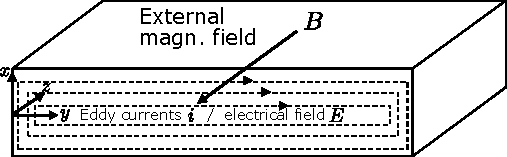
\includegraphics[width=0.95\textwidth]{fig/lec04/Eddy_currents_single_sheet.pdf}}
				\onslide<2->{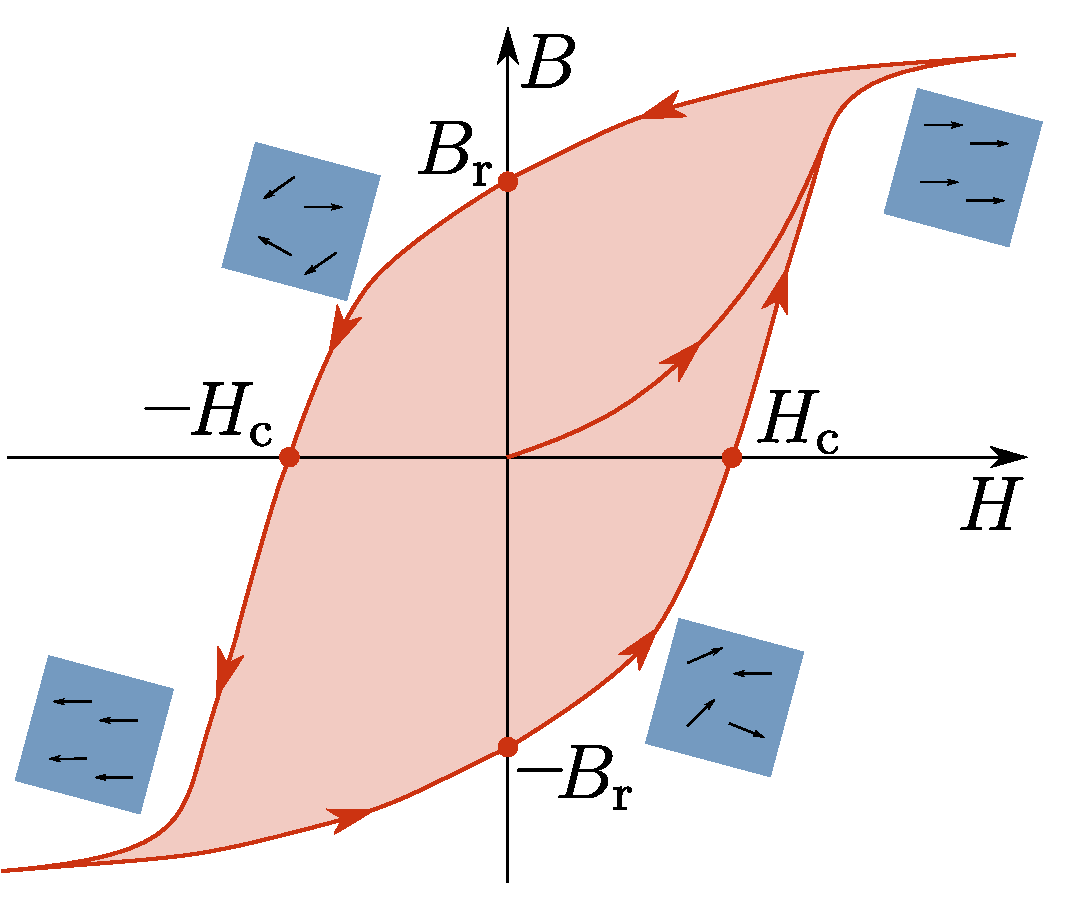
\includegraphics[width=0.95\textwidth]{fig/lec04/Hyteresis_curve_full.pdf}}

			\end{figure}
		\end{column}
		\begin{column}{0.6\textwidth}
			\onslide<1->{Iron losses in electrical machine cover (cf. right):}
			\begin{itemize}
				\item<1-> Eddy current losses: Due to time-varying magnetic fields, currents are induced in the iron core, leading to resistive losses.
				\item<2-> Hysteresis losses: Due to magnetic friction of changing orientation of Weiss domains.
			\end{itemize}\onslide<3->{%
					Empirical measurements show that the IM's iron losses can be approximated by
					\begin{equation}
						P_\mathrm{Fe}\approx \frac{1}{R_\mathrm{c}}\left\|\frac{\mathrm{d}}{\mathrm{d}t}\bm{\psi}^{\mathrm{s}}_{\mathrm{m},\upalpha\upbeta}\right\|^2=R_\mathrm{c}\left\|\bm{i}^{\mathrm{s}}_{\mathrm{c},\upalpha\upbeta}\right\|^2
					\end{equation}
					in the stator-oriented $\upalpha\upbeta$-frame, where $R_\mathrm{c}$ is an iron loss resistance and $\bm{i}^{\mathrm{s}}_{\mathrm{c},\upalpha\upbeta}$ is the iron loss current.}
		\end{column}
	\end{columns}
\end{frame}

%%%%%%%%%%%%%%%%%%%%%%%%%%%%%%%%%%%%%%%%%%%%%%%%%%%%%%%%%%%%%
%% T-type equivalent circuit model %%
%%%%%%%%%%%%%%%%%%%%%%%%%%%%%%%%%%%%%%%%%%%%%%%%%%%%%%%%%%%%%
\begin{frame}
	\frametitle{T-type equivalent circuit model with iron loss resistance}

	\begin{figure}
		\centering
		\begin{circuitikz}[straight voltages]

			% coordinates
			\coordinate (LT) at (0,2.5);
			\coordinate (LB) at (0,0);
			\coordinate (A)  at (1.0,2.5);
			\coordinate (B)  at (3.0,2.5);
			\coordinate (C)  at (5.0,2.5);
			\coordinate (N)  at (6.0,2.5);
			\coordinate (D)  at (8.0,2.5);
			\coordinate (E)  at (10.0,2.5);
			\coordinate (RT) at (11,2.5);
			\coordinate (RB) at (11.0,0);

			% main upper electrical path
			\draw
			(LT) to[short, i>^=$\bm{i}^{\mathrm{s}}_{\mathrm{s,\upalpha\upbeta}}$] (A)
			to[R, l=$R_{s}$] (B)
			to[L, l=$L_{\sigma \mathrm{s}}$] (C)
			to[short] (N)
			to[L, l=$L_{\sigma \mathrm{r}}$] (D)
			to[R, l=$R_{r}$] (E)
			to[short, i<^=$\underline{i}^{\mathrm{s}}_{\mathrm{r,\upalpha\upbeta}}$] (RT);

			% lower return path with rotational voltage sources
			\draw (LB) to [short] (C |- LB);
			\draw (N |- LB)  to [V, v_<=$\omega\bm{J}\bm{\psi}^{\mathrm{s}}_{\mathrm{r,\upalpha\upbeta}}$] (RB |- LB);
			\draw (N |- LB) to (C |- LB);

			% side connections
			\draw (LT) to[open, v=$\bm{u}^{\mathrm{s}}_{\mathrm{s,\upalpha\upbeta}}$, o-o] (LB);
			\draw (RT) to[short] (RB);

			% magnetizing branch
			\draw
			(C) to[L, l_=$L_{\mathrm{m}}$, i>_=$\bm{i}^{\mathrm{s}}_{\mathrm{m,\upalpha\upbeta}}$, *-*] (C |- LB);
			\draw
			(N) to[R, l=$R_{\mathrm{c}}$, i>^=$\bm{i}^{\mathrm{s}}_{\mathrm{c,\upalpha\upbeta}}$] (N |- LB);

			% connection dots
			\fill (N) circle[radius=1.6pt];
			\fill (N |- LB) circle[radius=1.6pt];

			% flux linkage voltage references
			\draw (3.2,2.5) to[open, v=$\frac{\mathrm{d}}{\mathrm{d}t}\bm{\psi}^{\mathrm{s}}_{\mathrm{s,\upalpha\upbeta}}$] (3.2,0);
			\draw (7.8,2.5) to[open, v^>=$\frac{\mathrm{d}}{\mathrm{d}t}\bm{\psi}^{\mathrm{s}}_{\mathrm{r,\upalpha\upbeta}}$] (7.8,0);
		\end{circuitikz}
		\caption{Extended T-type equivalent model with additional iron loss resistance $R_\mathrm{c}$ in the magnetizing branch depicted in the stator-oriented $\upalpha\upbeta$-frame}
		\label{fig:T_ECD_IM_iron_loss}
	\end{figure}
\end{frame}

%%%%%%%%%%%%%%%%%%%%%%%%%%%%%%%%%%%%%%%%%%%%%%%%%%%%%%%%%%%%%
%% No-load test for parameter identification %%
%%%%%%%%%%%%%%%%%%%%%%%%%%%%%%%%%%%%%%%%%%%%%%%%%%%%%%%%%%%%%
\begin{frame}
	\frametitle{No-load test for parameter identification}
	\onslide<2->{
			Assuming $R_\mathrm{s} << R_\mathrm{c}$ and $L_{\sigma\mathrm{s}}<<L_\mathrm{m}$, the mutual inductance and iron resistance can be identified from no-load active and reactive power measurements:
			\begin{equation}
				L_\mathrm{m}\approx 3\frac{U_\mathrm{s}^2}{Q_\mathrm{s}\omega }, \qquad
				R_\mathrm{c}\approx 3 \frac{U_\mathrm{s}^2}{P_\mathrm{s}},
			\end{equation}
			where $U_\mathrm{s}$ is the stator phase voltage RMS value at the applied angular frequency $\omega$ while $P_\mathrm{s}$ and $Q_\mathrm{s}$ are the active and reactive power measured at the stator, respectively.}
	\begin{figure}
		\begin{columns}
			\begin{column}{0.64\textwidth}
				\centering
				\begin{circuitikz}[straight voltages, scale=0.8, every node/.append style={scale=0.8}]

					% coordinates
					\coordinate (LT) at (0,2.5);
					\coordinate (LB) at (0,0);
					\coordinate (A)  at (1.0,2.5);
					\coordinate (B)  at (3.0,2.5);
					\coordinate (C)  at (5.0,2.5);
					\coordinate (N)  at (6.0,2.5);
					\coordinate (D)  at (8.0,2.5);
					\coordinate (E)  at (10.0,2.5);
					\coordinate (RT) at (11,2.5);
					\coordinate (RB) at (11.0,0);

					% main upper electrical path
					\draw
					(LT) to[short, i>^=$\bm{i}^{\mathrm{s}}_{\mathrm{s,\upalpha\upbeta}}$] (A)
					to[R, l=$R_{s}$] (B)
					to[L, l=$L_{\sigma \mathrm{s}}$] (C)
					to[short] (N);
					\draw[dashed] (N)
					to[L, l=$L_{\sigma \mathrm{r}}$] (D)
					to[R, l=$R_{r}$] (E)
					to[short, i<^=$\bm{i}^{\mathrm{s}}_{\mathrm{r,\upalpha\upbeta}} \approx 0$] (RT);

					% lower return path with rotational voltage sources
					\draw (LB) to [short] (C |- LB);
					\draw[dashed] (N |- LB)  to [V, v_<=$\omega\bm{J}\bm{\psi}^{\mathrm{s}}_{\mathrm{r,\upalpha\upbeta}}$] (RB |- LB);
					\draw (N |- LB) to (C |- LB);

					% side connections
					\draw (LT) to[open, v=$\bm{u}^{\mathrm{s}}_{\mathrm{s,\upalpha\upbeta}}$, o-o] (LB);
					\draw[dashed] (RT) to[short] (RB);

					% magnetizing branch
					\draw
					(C) to[L, l_=$L_{\mathrm{m}}$, i>_=$\bm{i}^{\mathrm{s}}_{\mathrm{m,\upalpha\upbeta}}$, *-*] (C |- LB);
					\draw
					(N) to[R, l=$R_{\mathrm{c}}$, i>^=$\bm{i}^{\mathrm{s}}_{\mathrm{c,\upalpha\upbeta}}$] (N |- LB);

					% connection dots
					\fill (N) circle[radius=1.6pt];
					\fill (N |- LB) circle[radius=1.6pt];

					% flux linkage voltage references
					\draw (3.2,2.5) to[open, v=$\frac{\mathrm{d}}{\mathrm{d}t}\bm{\psi}^{\mathrm{s}}_{\mathrm{s,\upalpha\upbeta}}$] (3.2,0);
					\draw (7.8,2.5) to[open, v^>=$\frac{\mathrm{d}}{\mathrm{d}t}\bm{\psi}^{\mathrm{s}}_{\mathrm{r,\upalpha\upbeta}}$] (7.8,0);
				\end{circuitikz}
			\end{column}
			\begin{column}{0.35\textwidth}
				\caption{\raggedright  No-load test (without a load the rotor runs synchronously to the stator field and thus the rotor current is approximately zero due to the lack of any rotor induced voltage)}
				\label{fig:T_ECD_IM_no_load_test}
			\end{column}
		\end{columns}
	\end{figure}
\end{frame}

%%%%%%%%%%%%%%%%%%%%%%%%%%%%%%%%%%%%%%%%%%%%%%%%%%%%%%%%%%%%%
%% Blocked rotor test for parameter identification %%
%%%%%%%%%%%%%%%%%%%%%%%%%%%%%%%%%%%%%%%%%%%%%%%%%%%%%%%%%%%%%
\begin{frame}
	\frametitle{Blocked rotor test for parameter identification}
	\onslide<2->{From a blocked rotor test with active and reactive power measurements we can approximate:
			\begin{equation}
				L_{\sigma\mathrm{s}}+L_{\sigma\mathrm{r}}\approx 3\frac{U_\mathrm{s}^2}{Q_\mathrm{s}\omega }, \qquad
				R_\mathrm{s} + R_\mathrm{r}\approx 3 \frac{U_\mathrm{s}^2}{P_\mathrm{s}}.
			\end{equation}}%
	\onslide<3->{With a separate ohmmeter  measurement of $R_\mathrm{s}$, the rotor resistance directly follows. However, for the stray inductances, further assumptions are required to split the sum into stator and rotor contributions (typically, $L_{\sigma\mathrm{s}}=L_{\sigma\mathrm{r}}$).}
	\begin{figure}
		\begin{columns}
			\begin{column}{0.64\textwidth}
				\centering
				\begin{circuitikz}[straight voltages, scale=0.8, every node/.append style={scale=0.8}]

					% coordinates
					\coordinate (LT) at (0,2.5);
					\coordinate (LB) at (0,0);
					\coordinate (A)  at (1.0,2.5);
					\coordinate (B)  at (3.0,2.5);
					\coordinate (C)  at (5.0,2.5);
					\coordinate (N)  at (6.0,2.5);
					\coordinate (D)  at (8.0,2.5);
					\coordinate (E)  at (10.0,2.5);
					\coordinate (RT) at (11,2.5);
					\coordinate (RB) at (11.0,0);

					% main upper electrical path
					\draw
					(LT) to[short, i>^=$\bm{i}^{\mathrm{s}}_{\mathrm{s,\upalpha\upbeta}}$] (A)
					to[R, l=$R_{s}$] (B)
					to[L, l=$L_{\sigma \mathrm{s}}$] (C)
					to[short] (N);
					\draw (N)
					to[L, l=$L_{\sigma \mathrm{r}}$] (D)
					to[R, l=$R_{r}$] (E)
					to[short, i<^=$\bm{i}^{\mathrm{s}}_{\mathrm{r,\upalpha\upbeta}}$] (RT);

					% lower return path with rotational voltage sources
					\draw (LB) to [short] (C |- LB);
					\draw (N |- LB)  to [V, v_<=$\omega\bm{J}\bm{\psi}^{\mathrm{s}}_{\mathrm{r,\upalpha\upbeta}}$] (RB |- LB);
					\draw (N |- LB) to (C |- LB);

					% side connections
					\draw (LT) to[open, v=$\bm{u}^{\mathrm{s}}_{\mathrm{s,\upalpha\upbeta}}$, o-o] (LB);
					\draw (RT) to[short] (RB);

					% magnetizing branch
					\draw[dashed]
					(C) to[L, l_=$L_{\mathrm{m}}$, i>_=$\bm{i}^{\mathrm{s}}_{\mathrm{m,\upalpha\upbeta}}\approx 0$, *-*] (C |- LB);
					\draw[dashed]
					(N) to[R, l=$R_{\mathrm{c}}$, i>^=$\bm{i}^{\mathrm{s}}_{\mathrm{c,\upalpha\upbeta}}\approx 0$] (N |- LB);

					% connection dots
					\fill (N) circle[radius=1.6pt];
					\fill (N |- LB) circle[radius=1.6pt];

					% flux linkage voltage references
					\draw (3.2,2.5) to[open, v=$\frac{\mathrm{d}}{\mathrm{d}t}\bm{\psi}^{\mathrm{s}}_{\mathrm{s,\upalpha\upbeta}}$] (3.2,0);
					\draw (7.8,2.5) to[open, v^>=$\frac{\mathrm{d}}{\mathrm{d}t}\bm{\psi}^{\mathrm{s}}_{\mathrm{r,\upalpha\upbeta}}$] (7.8,0);
				\end{circuitikz}
			\end{column}
			\begin{column}{0.35\textwidth}
				\caption{\raggedright  Blocked rotor test (analogous to a transformer's short-circuit test where high induced rotor currents dominate compared to the magnetizing branch)}
				\label{fig:T_ECD_IM_blocked_rotor_test}
			\end{column}
		\end{columns}
	\end{figure}
\end{frame}

%%%%%%%%%%%%%%%%%%%%%%%%%%%%%%%%%%%%%%%%%%%%%%%%%%%%%%%%%%%%%%%%%%
\subsection{Discrete-time machine models}
%%%%%%%%%%%%%%%%%%%%%%%%%%%%%%%%%%%%%%%%%%%%%%%%%%%%%%%%%%%%%%%%%%

%%%%%%%%%%%%%%%%%%%%%%%%%%%%%%%%%%%%%%%%%%%%%%%%%%%%%%%%%%%%%
%% Explicit Euler model in stator-oriented alpha-beta coordinates %%
%%%%%%%%%%%%%%%%%%%%%%%%%%%%%%%%%%%%%%%%%%%%%%%%%%%%%%%%%%%%%
\begin{frame}
	\frametitle{Nonlinear IM model in stator-oriented $\upalpha\upbeta$ coordinates}
	For deriving a discrete-time IM model, we follow the same route as in the previous PMSM case (first discretize, then rotate) and start in the \hl{stator-oriented} $\upalpha\upbeta$ coordinates for the stator flux while using the \hl{rotor-oriented} $\upalpha\upbeta$ coordinates for the rotor flux. The flux linkage ODEs in these coordinates are (based on Faradys's law):
	\begin{equation}
		\begin{split}
			\frac{\mathrm{d}}{\mathrm{d}t}\bm{\psi}^{\mathrm{s}}_\mathrm{s,\upalpha\upbeta}(t)
			 & = \bm{u}^{\mathrm{s}}_\mathrm{s,\upalpha\upbeta}(t)-R_\mathrm{s}\bm{i}^{\mathrm{s}}_\mathrm{s,\upalpha\upbeta}(t), \\
			\frac{\mathrm{d}}{\mathrm{d}t}\bm{\psi}^{\mathrm{r}}_\mathrm{r,\upalpha\upbeta}(t)
			 & = -R_\mathrm{r}\bm{i}^{\mathrm{r}}_\mathrm{r,\upalpha\upbeta}(t).
		\end{split}
		\label{eq:IM_alpha_beta_flux_ODE}
	\end{equation}\pause%
	Applying the \hl{explicit Euler method (RK1)} to \eqref{eq:IM_alpha_beta_flux_ODE} yields
	\begin{equation}
		\begin{split}
			\bm{\psi}^{\mathrm{s}}_\mathrm{s,\upalpha\upbeta}[k+1]
			 & =\bm{\psi}^{\mathrm{s}}_\mathrm{s,\upalpha\upbeta}[k]
			+T_\mathrm{s}\left(\bm{u}^{\mathrm{s}}_\mathrm{s,\upalpha\upbeta}[k]-R_\mathrm{s}\bm{i}^{\mathrm{s}}_\mathrm{s,\upalpha\upbeta}[k]\right), \\
			\bm{\psi}^{\mathrm{r}}_\mathrm{r,\upalpha\upbeta}[k+1]
			 & =\bm{\psi}^{\mathrm{r}}_\mathrm{r,\upalpha\upbeta}[k]
			+T_\mathrm{s}\left(-R_\mathrm{r}\bm{i}^{\mathrm{r}}_\mathrm{r,\upalpha\upbeta}[k]
			\right).
		\end{split}
		\label{eq:RK1_alpha_beta_flux_linkage_IM}
	\end{equation}
\end{frame}


%%%%%%%%%%%%%%%%%%%%%%%%%%%%%%%%%%%%%%%%%%%%%%%%%%%%%%%%%%%%%
%% Flux-based discrete-time IM model in general $\mathrm{k}$ coordinates %%
%%%%%%%%%%%%%%%%%%%%%%%%%%%%%%%%%%%%%%%%%%%%%%%%%%%%%%%%%%%%%
\begin{frame}
	\frametitle{Flux-based discrete-time IM model in general $\mathrm{k}$ coordinates}
	To obtain the model in a general $\mathrm{k}$ coordinate system, the RK1 update from \eqref{eq:RK1_alpha_beta_flux_linkage_IM} is transformed into a common frame via \hl{separate Park transformations}. Assuming approximately constant angular frequencies over one sampling interval gives
	\begin{equation}
		\begin{split}
			\bm{\psi}^{\mathrm{k}}_\mathrm{s,dq}[k+1]
			 & =\bm{T}_\mathrm{p}(-\omega_\mathrm{k}[k]T_\mathrm{s})
			\left(\bm{\psi}^{\mathrm{k}}_\mathrm{s,dq}[k]
			+T_\mathrm{s}\left(\bm{u}^{\mathrm{k}}_\mathrm{s,dq}[k]-R_\mathrm{s}\bm{i}^{\mathrm{k}}_\mathrm{s,dq}[k]\right)\right), \\[0.5ex]
			\bm{\psi}^{\mathrm{k}}_\mathrm{r,dq}[k+1]
			 & =\bm{T}_\mathrm{p}((\omega[k]-\omega_\mathrm{k}[k])T_\mathrm{s})
			\left(\bm{\psi}^{\mathrm{k}}_\mathrm{r,dq}[k]
			-T_\mathrm{s}R_\mathrm{r}\bm{i}^{\mathrm{k}}_\mathrm{r,dq}[k]
			\right).
		\end{split}
		\label{eq:RK1_k_flux_linkage_IM}
	\end{equation}\pause%
	The rotation matrix $\bm{T}_\mathrm{p}(-\omega_\mathrm{k}[k]T_\mathrm{s})$ represents the change of the reference frame between $k$ and $k+1$ from the stator point of view, while $\bm{T}_\mathrm{p}((\omega[k]-\omega_\mathrm{k}[k])T_\mathrm{s})$ represents the change of the reference frame between $k$ and $k+1$ from the rotor point of view, i.e., the slip frequency. \pause The \hl{electromagnetic torque} remains
	\begin{equation}
		T[k]=\frac{3}{2}p\left(\bm{i}^{\mathrm{k}}_\mathrm{s,dq}[k]\right)\T\bm{J}\bm{\psi}^{\mathrm{k}}_\mathrm{s,dq}[k]
		=-\frac{3}{2}p\left(\bm{i}^{\mathrm{k}}_\mathrm{r,dq}[k]\right)\T\bm{J}\bm{\psi}^{\mathrm{k}}_\mathrm{r,dq}[k].
		\label{eq:discrete_time_IM_torque}    \end{equation}
\end{frame}

%%%%%%%%%%%%%%%%%%%%%%%%%%%%%%%%%%%%%%%%%%%%%%%%%%%%%%%%%%%%%
%% Condensed flux-based model %%
%%%%%%%%%%%%%%%%%%%%%%%%%%%%%%%%%%%%%%%%%%%%%%%%%%%%%%%%%%%%%
\begin{frame}
	\frametitle{Condensed flux-based discrete-time IM model}
	With condensed notation for the flux linkages, currents, voltages, resistances and discrete rotations as
	\begin{equation}
		\begin{gathered}
			\bm{\psi}^{\mathrm{k}}_\mathrm{dq}=\begin{bmatrix}
				\bm{\psi}^{\mathrm{k}}_{\mathrm{s,dq}} \\
				\bm{\psi}^{\mathrm{k}}_{\mathrm{r,dq}}
			\end{bmatrix},\qquad
			\bm{i}^{\mathrm{k}}_\mathrm{dq}=\begin{bmatrix}
				\bm{i}^{\mathrm{k}}_{\mathrm{s,dq}} \\
				\bm{i}^{\mathrm{k}}_{\mathrm{r,dq}}
			\end{bmatrix},\qquad
			\bm{u}^{\mathrm{k}}_\mathrm{dq}=\begin{bmatrix}
				\bm{u}^{\mathrm{k}}_{\mathrm{s,dq}} \\
				\bm{0}_{2\times 1}
			\end{bmatrix},\\[1ex]
			\bm{R}_\mathrm{dq}=\begin{bmatrix}
				R_\mathrm{s}\bm{I}_2 & \bm{0}_{2\times 2}   \\
				\bm{0}_{2\times 2}   & R_\mathrm{r}\bm{I}_2
			\end{bmatrix},\qquad
			\bm{T}_\mathrm{dq}[k]=\begin{bmatrix}
				\bm{T}_\mathrm{p}(-\omega_\mathrm{k}[k]T_\mathrm{s}) & \bm{0}_{2\times 2}                                              \\
				\bm{0}_{2\times 2}                                   & \bm{T}_\mathrm{p}((\omega[k]-\omega_\mathrm{k}[k])T_\mathrm{s})
			\end{bmatrix},
		\end{gathered}
		\label{eq:IM_dt_condensed_notation}
	\end{equation}\pause%
	the \hl{condensed flux-based difference equation in a general $\mathrm{k}$ coordinate system} is
	\begin{equation}
		\bm{\psi}^{\mathrm{k}}_\mathrm{dq}[k+1]
		=\bm{T}_\mathrm{dq}[k]\Big(\bm{\psi}^{\mathrm{k}}_\mathrm{dq}[k]
		+T_\mathrm{s}(\bm{u}^{\mathrm{k}}_\mathrm{dq}[k]-\bm{R}_\mathrm{dq}\bm{i}^{\mathrm{k}}_\mathrm{dq}[k])\Big).
		\label{eq:IM_dt_flux_based_condensed}
	\end{equation}
\end{frame}

%%%%%%%%%%%%%%%%%%%%%%%%%%%%%%%%%%%%%%%%%%%%%%%%%%%%%%%%%%%%%
%% Current-based nonlinear model %%
%%%%%%%%%%%%%%%%%%%%%%%%%%%%%%%%%%%%%%%%%%%%%%%%%%%%%%%%%%%%%
\begin{frame}
	\frametitle{Current-based discrete-time IM model}
	For a current-based representation, the local nonlinear flux increment is approximated by the combined differential inductance matrix from \eqref{eq:full_differential_inductance_matrix}:
	\begin{equation}
		\bm{\psi}^{\mathrm{k}}_\mathrm{dq}[k+1]-\bm{\psi}^{\mathrm{k}}_\mathrm{dq}[k]
		\approx\bm{L}\!\left(\bm{i}^{\mathrm{k}}_\mathrm{dq}[k]\right)
		\left(\bm{i}^{\mathrm{k}}_\mathrm{dq}[k+1]-\bm{i}^{\mathrm{k}}_\mathrm{dq}[k]\right).
		\label{eq:IM_dt_current_increment}
	\end{equation}\pause%
	Applying this to \eqref{eq:IM_dt_flux_based_condensed} and solving for $\bm{i}^{\mathrm{k}}_\mathrm{dq}[k+1]$ yields
	\begin{equation}
		\begin{split}
			\bm{i}^{\mathrm{k}}_\mathrm{dq}[k+1]
			 & =\bm{i}^{\mathrm{k}}_\mathrm{dq}[k]
			+\bm{L}^{-1}[k]\Bigg(\!\left[
				                       \begin{array}{cc}
					                       \bm{T}_\mathrm{p}(-\omega_\mathrm{k}[k]T_\mathrm{s}) & \bm{0}                                                          \\
					                       \bm{0}                                               & \bm{T}_\mathrm{p}((\omega[k]-\omega_\mathrm{k}[k])T_\mathrm{s})
				                       \end{array}\right]-\bm{I}_4\!\Bigg)\bm{\psi}^{\mathrm{k}}_\mathrm{dq}[k] \\
			 & \quad+\bm{L}^{-1}[k]\left[
				                       \begin{array}{cc}
					                       \bm{T}_\mathrm{p}(-\omega_\mathrm{k}[k]T_\mathrm{s}) & \bm{0}                                                          \\
					                       \bm{0}                                               & \bm{T}_\mathrm{p}((\omega[k]-\omega_\mathrm{k}[k])T_\mathrm{s})
				                       \end{array}\right]T_\mathrm{s}
			\begin{bmatrix}
				\bm{u}^{\mathrm{k}}_{\mathrm{s,dq}}[k]-R_\mathrm{s}\bm{i}^{\mathrm{k}}_{\mathrm{s,dq}}[k] \\
				-R_\mathrm{r}\bm{i}^{\mathrm{k}}_{\mathrm{r,dq}}[k]
			\end{bmatrix} .
		\end{split}
		\label{eq:IM_dt_current_based_detailed}
	\end{equation}\pause%
	Here, $\bm{L}[k]=\bm{L}(\bm{i}^{\mathrm{k}}_\mathrm{dq}[k])$ is the differential inductance matrix.
\end{frame}


%%%%%%%%%%%%%%%%%%%%%%%%%%%%%%%%%%%%%%%%%%%%%%%%%%%%%%%%%%%%%
%% Detailed current difference equation interpretation %%
%%%%%%%%%%%%%%%%%%%%%%%%%%%%%%%%%%%%%%%%%%%%%%%%%%%%%%%%%%%%%
\begin{frame}
	\frametitle{Current difference equation of the nonlinear IM model (cont.)}
	Equation \eqref{eq:IM_dt_current_based_detailed} can be interpreted as the sum of three contributions:
	\begin{equation}
		\begin{split}
			\bm{i}^{\mathrm{k}}_\mathrm{dq}[k+1]
			 & =
			\underbrace{\bm{i}^{\mathrm{k}}_\mathrm{dq}[k]-\bm{L}^{-1}[k]T_\mathrm{s}
				\begin{bmatrix}
					\bm{T}_\mathrm{p}(-\omega_\mathrm{k}[k]T_\mathrm{s})R_\mathrm{s}\bm{i}^{\mathrm{k}}_{\mathrm{s,dq}}[k] \\
					\bm{T}_\mathrm{p}((\omega[k]-\omega_\mathrm{k}[k])T_\mathrm{s})R_\mathrm{r}\bm{i}^{\mathrm{k}}_{\mathrm{r,dq}}[k]
				\end{bmatrix}}_{\text{first-order delay / PT1 eigendynamics}}                 \\
			 & \quad+\underbrace{\bm{L}^{-1}[k]\Bigg(\!\left[
					         \begin{array}{cc}
						         \bm{T}_\mathrm{p}(-\omega_\mathrm{k}[k]T_\mathrm{s}) & \bm{0}                                                          \\
						         \bm{0}                                               & \bm{T}_\mathrm{p}((\omega[k]-\omega_\mathrm{k}[k])T_\mathrm{s})
					         \end{array}\right]-\bm{I}_4\!\Bigg)\bm{\psi}^{\mathrm{k}}_\mathrm{dq}[k]}_{\text{equiv. induced voltage contribution}} \\
			 & \quad+\underbrace{\bm{L}^{-1}[k]T_\mathrm{s}
				         \begin{bmatrix}
					         \bm{T}_\mathrm{p}(-\omega_\mathrm{k}[k]T_\mathrm{s})\bm{u}^{\mathrm{k}}_{\mathrm{s,dq}}[k] \\
					         \bm{0}
				         \end{bmatrix}}_{\text{input voltage contribution}} .
		\end{split}
		\label{eq:IM_dt_current_based_interpretation}
	\end{equation}
\end{frame}

%%%%%%%%%%%%%%%%%%%%%%%%%%%%%%%%%%%%%%%%%%%%%%%%%%%%%%%%%%%%%
%% Starting point %%
%%%%%%%%%%%%%%%%%%%%%%%%%%%%%%%%%%%%%%%%%%%%%%%%%%%%%%%%%%%%%
\begin{frame}
	\frametitle{Rotor-flux-oriented discrete-time IM model: starting point}
	\begin{varblock}{Objective}
		In the following, we derive a rotor-flux-oriented discrete-time IM model ($\mathrm{k}=\psi_\mathrm{r}$) for field-oriented control purpose. As a goal we aim for a model with the states $\bm{x}^\top=[\psi^{\psi_\mathrm{r}}_{\mathrm{r,d}},\, i^{\psi_\mathrm{r}}_{\mathrm{s,d}},\, i^{\psi_\mathrm{r}}_{\mathrm{s,q}}]$ assuming an accurate stator current measurement and an accurate rotor flux estimation.
	\end{varblock}\pause%
	The derivation starts from the common $\mathrm{k}$-coordinate flux difference equations:
	\begin{equation*}
		\bm{\psi}^{\mathrm{k}}_{\mathrm{s,dq}}[k+1]
		=\bm{T}_\mathrm{p}(-\omega_\mathrm{k}[k]T_\mathrm{s})
		\left(\bm{\psi}^{\mathrm{k}}_{\mathrm{s,dq}}[k]
		+T_\mathrm{s}\left(\bm{u}^{\mathrm{k}}_{\mathrm{s,dq}}[k]
		-R_\mathrm{s}\bm{i}^{\mathrm{k}}_{\mathrm{s,dq}}[k]\right)\right),
	\end{equation*}
	\begin{equation*}
		\bm{\psi}^{\mathrm{k}}_{\mathrm{r,dq}}[k+1]
		=\bm{T}_\mathrm{p}((\omega[k]-\omega_\mathrm{k}[k])T_\mathrm{s})
		\left(\bm{\psi}^{\mathrm{k}}_{\mathrm{r,dq}}[k]
		-T_\mathrm{s}R_\mathrm{r}\bm{i}^{\mathrm{k}}_{\mathrm{r,dq}}[k]\right).
	\end{equation*}\pause%
	From the rotor flux orientation condition, the rotor flux is aligned with the $\mathrm{d}$-axis at each sampling instant:
	\begin{equation}
		\bm{\psi}^{\psi_\mathrm{r}}_{\mathrm{r,dq}}[k]
		=\begin{bmatrix}\psi^{\psi_\mathrm{r}}_{\mathrm{r,d}}[k]\\0\end{bmatrix}.
		\label{eq:IM_RFO_v5_orientation}
	\end{equation}
\end{frame}

%%%%%%%%%%%%%%%%%%%%%%%%%%%%%%%%%%%%%%%%%%%%%%%%%%%%%%%%%%%%%
%% Rotor current elimination %%
%%%%%%%%%%%%%%%%%%%%%%%%%%%%%%%%%%%%%%%%%%%%%%%%%%%%%%%%%%%%%
\begin{frame}
	\frametitle{Rotor flux orientation: rotor current elimination}
	The apparent-inductance rotor flux relation from the nonlinear IM model is\footnote{We drop the explicit current dependence of the apparent inductances for readability and just use the time index $k$ to indicate the non-constant nature of the inductances: $L^{\psi_\mathrm{r}}_{\mathrm{m,app}}[k]=L^{\psi_\mathrm{r}}_{\mathrm{m,app}}(\bm{i}^{\psi_\mathrm{r}}_{\mathrm{s,dq}}[k],\bm{i}^{\psi_\mathrm{r}}_{\mathrm{r,dq}}[k]), \ldots$ }:
	\begin{equation}
		\bm{\psi}^{\psi_\mathrm{r}}_{\mathrm{r,dq}}[k]
		=L^{\psi_\mathrm{r}}_{\mathrm{m,app}}[k]\bm{i}^{\psi_\mathrm{r}}_{\mathrm{s,dq}}[k]
		+\left(L^{\psi_\mathrm{r}}_{\mathrm{m,app}}[k]+L^{\psi_\mathrm{r}}_{\sigma\mathrm{r,app}}[k]\right)
		\bm{i}^{\psi_\mathrm{r}}_{\mathrm{r,dq}}[k].
		\label{eq:IM_RFO_v5_apparent_rotor_flux}
	\end{equation}\pause%
	Using \eqref{eq:IM_RFO_v5_orientation} gives
	\begin{equation}
		\begin{split}
			i^{\psi_\mathrm{r}}_{\mathrm{r,d}}[k]
			 & =\frac{\psi^{\psi_\mathrm{r}}_{\mathrm{r,d}}[k]
				    -L^{\psi_\mathrm{r}}_{\mathrm{m,app}}[k]i^{\psi_\mathrm{r}}_{\mathrm{s,d}}[k]}
			    {L^{\psi_\mathrm{r}}_{\mathrm{m,app}}[k]+L^{\psi_\mathrm{r}}_{\sigma\mathrm{r,app}}[k]}, \\[0.6ex]
			i^{\psi_\mathrm{r}}_{\mathrm{r,q}}[k]
			 & =-\frac{L^{\psi_\mathrm{r}}_{\mathrm{m,app}}[k]}
			     {L^{\psi_\mathrm{r}}_{\mathrm{m,app}}[k]+L^{\psi_\mathrm{r}}_{\sigma\mathrm{r,app}}[k]}
			i^{\psi_\mathrm{r}}_{\mathrm{s,q}}[k].
		\end{split}
		\label{eq:IM_RFO_v5_rotor_current_elimination}
	\end{equation}
\end{frame}

%%%%%%%%%%%%%%%%%%%%%%%%%%%%%%%%%%%%%%%%%%%%%%%%%%%%%%%%%%%%%
%% Rotor flux rotation %%
%%%%%%%%%%%%%%%%%%%%%%%%%%%%%%%%%%%%%%%%%%%%%%%%%%%%%%%%%%%%%
\begin{frame}
	\frametitle{Rotor flux orientation: transformed rotor flux step}
	Applying \eqref{eq:IM_RFO_v5_orientation} to the rotor flux difference equation yields
	\begin{equation}
		\begin{bmatrix}\psi^{\psi_\mathrm{r}}_{\mathrm{r,d}}[k+1]\\0\end{bmatrix}
		=\bm{T}_\mathrm{p}(-\omega_\mathrm{slip}[k]T_\mathrm{s})
		\left(
		\begin{bmatrix}\psi^{\psi_\mathrm{r}}_{\mathrm{r,d}}[k]\\0\end{bmatrix}
		-T_\mathrm{s}R_\mathrm{r}
		\begin{bmatrix}i^{\psi_\mathrm{r}}_{\mathrm{r,d}}[k]\\i^{\psi_\mathrm{r}}_{\mathrm{r,q}}[k]\end{bmatrix}
		\right),
		\label{eq:IM_RFO_v5_rotor_flux_rotated}
	\end{equation}
	with $\omega_\mathrm{slip}[k]=\omega_{\psi_\mathrm{r}}[k]-\omega[k]$ \pause Hence, both components after the Euler step are affected by the rotation:
	\begin{equation}
		\begin{split}
			\psi^{\psi_\mathrm{r}}_{\mathrm{r,d}}[k+1]
			  & =\cos(-\omega_\mathrm{slip}[k]T_\mathrm{s})
			\left(\psi^{\psi_\mathrm{r}}_{\mathrm{r,d}}[k]-T_\mathrm{s}R_\mathrm{r}i^{\psi_\mathrm{r}}_{\mathrm{r,d}}[k]\right) \\
			  & \quad+\sin(-\omega_\mathrm{slip}[k]T_\mathrm{s})T_\mathrm{s}R_\mathrm{r}i^{\psi_\mathrm{r}}_{\mathrm{r,q}}[k],  \\
			0 & =\sin(-\omega_\mathrm{slip}[k]T_\mathrm{s})
			\left(\psi^{\psi_\mathrm{r}}_{\mathrm{r,d}}[k]-T_\mathrm{s}R_\mathrm{r}i^{\psi_\mathrm{r}}_{\mathrm{r,d}}[k]\right) \\
			  & \quad-\cos(-\omega_\mathrm{slip}[k]T_\mathrm{s})T_\mathrm{s}R_\mathrm{r}i^{\psi_\mathrm{r}}_{\mathrm{r,q}}[k].
		\end{split}
		\label{eq:IM_RFO_v5_rotor_flux_components}
	\end{equation}
\end{frame}

%%%%%%%%%%%%%%%%%%%%%%%%%%%%%%%%%%%%%%%%%%%%%%%%%%%%%%%%%%%%%
%% Slip frequency %%
%%%%%%%%%%%%%%%%%%%%%%%%%%%%%%%%%%%%%%%%%%%%%%%%%%%%%%%%%%%%%
\begin{frame}
	\frametitle{Rotor flux orientation: slip angular frequency}
	From the $\mathrm{q}$-axis condition in \eqref{eq:IM_RFO_v5_rotor_flux_components} follows
	\begin{equation}
		\tan(-\omega_\mathrm{slip}[k]T_\mathrm{s})
		=\frac{T_\mathrm{s}R_\mathrm{r}i^{\psi_\mathrm{r}}_{\mathrm{r,q}}[k]}
		{\psi^{\psi_\mathrm{r}}_{\mathrm{r,d}}[k]-T_\mathrm{s}R_\mathrm{r}i^{\psi_\mathrm{r}}_{\mathrm{r,d}}[k]}.
		\label{eq:IM_RFO_v5_slip_before_elimination}
	\end{equation}\pause%
	Inserting \eqref{eq:IM_RFO_v5_rotor_current_elimination} yields the \hl{discrete-time slip expression}
	\begin{equation}
		\begin{split}
			\omega_\mathrm{slip}[k]
			=\frac{1}{T_\mathrm{s}}\operatorname{atan2}\left(
			T_\mathrm{s}R_\mathrm{r}\frac{L^{\psi_\mathrm{r}}_{\mathrm{m,app}}[k]}
			                        {L^{\psi_\mathrm{r}}_{\mathrm{m,app}}[k]+L^{\psi_\mathrm{r}}_{\sigma\mathrm{r,app}}[k]}
			i^{\psi_\mathrm{r}}_{\mathrm{s,q}}[k], \right. \\
			\left.
			\psi^{\psi_\mathrm{r}}_{\mathrm{r,d}}[k]
			-T_\mathrm{s}R_\mathrm{r}\frac{\psi^{\psi_\mathrm{r}}_{\mathrm{r,d}}[k]
				                         -L^{\psi_\mathrm{r}}_{\mathrm{m,app}}[k]i^{\psi_\mathrm{r}}_{\mathrm{s,d}}[k]}
			                         {L^{\psi_\mathrm{r}}_{\mathrm{m,app}}[k]+L^{\psi_\mathrm{r}}_{\sigma\mathrm{r,app}}[k]}
			\right).
			\label{eq:IM_RFO_v5_slip_after_elimination}
		\end{split}
	\end{equation}
\end{frame}

%%%%%%%%%%%%%%%%%%%%%%%%%%%%%%%%%%%%%%%%%%%%%%%%%%%%%%%%%%%%%
%% Continuous-time limit of slip frequency %%
%%%%%%%%%%%%%%%%%%%%%%%%%%%%%%%%%%%%%%%%%%%%%%%%%%%%%%%%%%%%%
\begin{frame}
	\frametitle{Rotor flux orientation: continuous-time limit}
	For fixed \(\psi^{\psi_\mathrm{r}}_{\mathrm{r,d}}[k]>0\), \(i^{\psi_\mathrm{r}}_{\mathrm{r,d}}[k]\) and \(i^{\psi_\mathrm{r}}_{\mathrm{r,q}}[k]\), the \(\operatorname{atan2}\) expression locally equals
	\begin{equation}
		\omega_\mathrm{slip}(T_\mathrm{s})=\frac{1}{T_\mathrm{s}}
		\arctan\!\left(
		\frac{-T_\mathrm{s}R_\mathrm{r}i^{\psi_\mathrm{r}}_{\mathrm{r,q}}[k]}
		{\psi^{\psi_\mathrm{r}}_{\mathrm{r,d}}[k]-T_\mathrm{s}R_\mathrm{r}i^{\psi_\mathrm{r}}_{\mathrm{r,d}}[k]}
		\right).
		\label{eq:IM_dt_RFO_slip_limit_start}
	\end{equation}\pause%
	With \(f(T_\mathrm{s})=\arctan(\cdot)\), L'Hospital's rule gives
	\begin{equation}
		\lim_{T_\mathrm{s}\rightarrow 0}\omega_\mathrm{slip}(T_\mathrm{s})
		=-\lim_{T_\mathrm{s}\rightarrow 0}\frac{f(T_\mathrm{s})}{T_\mathrm{s}}
		=-f'(0)=-\frac{R_\mathrm{r}i^{\psi_\mathrm{r}}_{\mathrm{r,q}}[k]}
		{\psi^{\psi_\mathrm{r}}_{\mathrm{r,d}}[k]}.
		\label{eq:IM_dt_RFO_slip_limit_rotor_current}
	\end{equation}\pause%
	This is identical to the continuous-time slip frequency from \eqref{eq:IM_model_k_rotor_flux_orientation_angular_velocity}, showing that the discrete-time rotor flux model consistently approximates the continuous-time model for small sampling times.
\end{frame}

%%%%%%%%%%%%%%%%%%%%%%%%%%%%%%%%%%%%%%%%%%%%%%%%%%%%%%%%%%%%%
%% Rotor flux state difference equation %%
%%%%%%%%%%%%%%%%%%%%%%%%%%%%%%%%%%%%%%%%%%%%%%%%%%%%%%%%%%%%%
\begin{frame}
	\frametitle{Rotor flux difference equation in rotor flux coordinates}
	Substitution of \eqref{eq:IM_RFO_v5_rotor_current_elimination} into the $\mathrm{d}$-axis component of \eqref{eq:IM_RFO_v5_rotor_flux_components} gives
	\begin{equation}
		\begin{split}
			\psi^{\psi_\mathrm{r}}_{\mathrm{r,d}}[k+1]
			 & =\cos(\omega_\mathrm{slip}[k]T_\mathrm{s})
			\left(\psi^{\psi_\mathrm{r}}_{\mathrm{r,d}}[k]
			-T_\mathrm{s}R_\mathrm{r}
			\frac{\psi^{\psi_\mathrm{r}}_{\mathrm{r,d}}[k]
				-L^{\psi_\mathrm{r}}_{\mathrm{m,app}}[k]i^{\psi_\mathrm{r}}_{\mathrm{s,d}}[k]}
			{L^{\psi_\mathrm{r}}_{\mathrm{m,app}}[k]+L^{\psi_\mathrm{r}}_{\sigma\mathrm{r,app}}[k]}\right) \\
			 & \quad-\sin(\omega_\mathrm{slip}[k]T_\mathrm{s})T_\mathrm{s}R_\mathrm{r}
			\frac{L^{\psi_\mathrm{r}}_{\mathrm{m,app}}[k]}
			{L^{\psi_\mathrm{r}}_{\mathrm{m,app}}[k]+L^{\psi_\mathrm{r}}_{\sigma\mathrm{r,app}}[k]}
			i^{\psi_\mathrm{r}}_{\mathrm{s,q}}[k].
		\end{split}\
		\label{eq:IM_RFO_v5_rotor_flux_exact}
	\end{equation}\pause%
	However, the slip frequency $\omega_\mathrm{slip}[k]$ is typically quite small (e.g., in the order of a few tens of rad/s) and the sampling time $T_\mathrm{s}$ is in the order of hundred microseconds, so that $\omega_\mathrm{slip}[k]T_\mathrm{s}\ll 1$ holds. Applying the \hl{small-angle approximation} $\cos(\omega_\mathrm{slip}[k]T_\mathrm{s})\approx1$ and $\sin(\omega_\mathrm{slip}[k]T_\mathrm{s})\approx0$ is therefore well justified and leads to the \hl{rotor flux difference equation}:
	\begin{equation}
		\psi^{\psi_\mathrm{r}}_{\mathrm{r,d}}[k+1]
		=\left(1-\frac{T_\mathrm{s}R_\mathrm{r}}
		{L^{\psi_\mathrm{r}}_{\mathrm{m,app}}[k]+L^{\psi_\mathrm{r}}_{\sigma\mathrm{r,app}}[k]}\right)
		\psi^{\psi_\mathrm{r}}_{\mathrm{r,d}}[k]
		\quad+\frac{T_\mathrm{s}R_\mathrm{r}L^{\psi_\mathrm{r}}_{\mathrm{m,app}}[k]}
		{L^{\psi_\mathrm{r}}_{\mathrm{m,app}}[k]+L^{\psi_\mathrm{r}}_{\sigma\mathrm{r,app}}[k]}
		i^{\psi_\mathrm{r}}_{\mathrm{s,d}}[k].
		\label{eq:IM_RFO_v5_rotor_flux_first_order}
	\end{equation}
\end{frame}

%%%%%%%%%%%%%%%%%%%%%%%%%%%%%%%%%%%%%%%%%%%%%%%%%%%%%%%%%%%%%
%% Starting point for the current difference equation %%
%%%%%%%%%%%%%%%%%%%%%%%%%%%%%%%%%%%%%%%%%%%%%%%%%%%%%%%%%%%%%
\begin{frame}
	\frametitle{Starting point for the current difference equation}
	In rotor-flux-oriented coordinates, the stator part of the common $\mathrm{k}$-frame flux difference equation reads
	\begin{equation*}
		\bm{\psi}^{\psi_\mathrm{r}}_{\mathrm{s},\mathrm{dq}}[k+1]
		=\bm{T}_\mathrm{p}(-\omega_{\psi_\mathrm{r}}[k]T_\mathrm{s})\left(\bm{\psi}^{\psi_\mathrm{r}}_{\mathrm{s},\mathrm{dq}}[k]
		+T_\mathrm{s}\left(\bm{u}^{\psi_\mathrm{r}}_{\mathrm{s},\mathrm{dq}}[k]
		-R_\mathrm{s}\bm{i}^{\psi_\mathrm{r}}_{\mathrm{s},\mathrm{dq}}[k]\right)\right).
	\end{equation*}\pause%
	Hence, with $\Delta\bm{\psi}^{\psi_\mathrm{r}}_{\mathrm{s},\mathrm{dq}}[k]=\bm{\psi}^{\psi_\mathrm{r}}_{\mathrm{s},\mathrm{dq}}[k+1]-\bm{\psi}^{\psi_\mathrm{r}}_{\mathrm{s},\mathrm{dq}}[k]$,
	\begin{equation}
		\begin{split}
			\Delta\bm{\psi}^{\psi_\mathrm{r}}_{\mathrm{s},\mathrm{dq}}[k]
			 & =\left(\bm{T}_\mathrm{p}(-\omega_{\psi_\mathrm{r}}[k]T_\mathrm{s})-\bm{I}_2\right)\bm{\psi}^{\psi_\mathrm{r}}_{\mathrm{s},\mathrm{dq}}[k] \\
			 & \quad+T_\mathrm{s}\bm{T}_\mathrm{p}(-\omega_{\psi_\mathrm{r}}[k]T_\mathrm{s})
			\left(\bm{u}^{\psi_\mathrm{r}}_{\mathrm{s},\mathrm{dq}}[k]
			-R_\mathrm{s}\bm{i}^{\psi_\mathrm{r}}_{\mathrm{s},\mathrm{dq}}[k]\right).
		\end{split}
		\label{eq:IM_RFO_v7_stator_flux_increment}
	\end{equation}\pause%
	The goal is to transform \eqref{eq:IM_RFO_v7_stator_flux_increment} into a current difference equation without an independent stator flux state.
\end{frame}



%%%%%%%%%%%%%%%%%%%%%%%%%%%%%%%%%%%%%%%%%%%%%%%%%%%%%%%%%%%%%
%% Stator flux as algebraic function of the states %%
%%%%%%%%%%%%%%%%%%%%%%%%%%%%%%%%%%%%%%%%%%%%%%%%%%%%%%%%%%%%%
\begin{frame}
	\frametitle{Stator flux as algebraic function of the states}
	The apparent stator flux relation is
	\begin{equation*}
		\bm{\psi}^{\psi_\mathrm{r}}_{\mathrm{s},\mathrm{dq}}[k]
		=L^{\psi_\mathrm{r}}_{\mathrm{m},\mathrm{app}}[k]
		\left(\bm{i}^{\psi_\mathrm{r}}_{\mathrm{s},\mathrm{dq}}[k]+\bm{i}^{\psi_\mathrm{r}}_{\mathrm{r},\mathrm{dq}}[k]\right)
		+L^{\psi_\mathrm{r}}_{\sigma\mathrm{s},\mathrm{app}}[k]\bm{i}^{\psi_\mathrm{r}}_{\mathrm{s},\mathrm{dq}}[k].
		\label{eq:IM_RFO_v7_stator_app_relation}
	\end{equation*}\pause%
	Inserting \eqref{eq:total_flux_model_explicit} and \eqref{eq:IM_RFO_v5_rotor_current_elimination} gives
	\begin{equation}
		\begin{split}
			\psi^{\psi_\mathrm{r}}_{\mathrm{s},\mathrm{d}}[k]
			 & =\frac{L^{\psi_\mathrm{r}}_{\mathrm{m},\mathrm{app}}[k]}
			    {L^{\psi_\mathrm{r}}_{\mathrm{m},\mathrm{app}}[k]+L^{\psi_\mathrm{r}}_{\sigma\mathrm{r},\mathrm{app}}[k]}
			\psi^{\psi_\mathrm{r}}_{\mathrm{r},\mathrm{d}} +\left(L^{\psi_\mathrm{r}}_{\sigma\mathrm{s},\mathrm{app}}[k]
			+\frac{L^{\psi_\mathrm{r}}_{\mathrm{m},\mathrm{app}}[k]L^{\psi_\mathrm{r}}_{\sigma\mathrm{r},\mathrm{app}}[k]}
			 {L^{\psi_\mathrm{r}}_{\mathrm{m},\mathrm{app}}[k]+L^{\psi_\mathrm{r}}_{\sigma\mathrm{r},\mathrm{app}}[k]}\right)i^{\psi_\mathrm{r}}_{\mathrm{s},\mathrm{d}}[k], \\[0.5ex]
			\psi^{\psi_\mathrm{r}}_{\mathrm{s},\mathrm{q}}[k]
			 & =\left(L^{\psi_\mathrm{r}}_{\sigma\mathrm{s},\mathrm{app}}[k]
			+\frac{L^{\psi_\mathrm{r}}_{\mathrm{m},\mathrm{app}}[k]L^{\psi_\mathrm{r}}_{\sigma\mathrm{r},\mathrm{app}}[k]}
			 {L^{\psi_\mathrm{r}}_{\mathrm{m},\mathrm{app}}[k]+L^{\psi_\mathrm{r}}_{\sigma\mathrm{r},\mathrm{app}}[k]}\right)i^{\psi_\mathrm{r}}_{\mathrm{s},\mathrm{q}}[k].
		\end{split}
		\label{eq:IM_RFO_v7_stator_flux_state_expr}
	\end{equation}
	With the stray constant $\sigma$ from \eqref{eq:stray_constant_def}  and \eqref{eq:IM_currents_stray_constant_def}, the stator flux can be expressed as
	\begin{equation}
		\bm{\psi}^{\psi_\mathrm{r}}_{\mathrm{s},\mathrm{dq}}[k] = \sigma[k] L^{\psi_\mathrm{r}}_{\mathrm{s},\mathrm{app}}[k]\bm{i}^{\psi_\mathrm{r}}_{\mathrm{s},\mathrm{dq}}[k] + \frac{L^{\psi_\mathrm{r}}_{\mathrm{m},\mathrm{app}}[k]}{L^{\psi_\mathrm{r}}_{\mathrm{r},\mathrm{app}}[k]}\psi^{\psi_\mathrm{r}}_{\mathrm{r},\mathrm{d}}[k].
		\label{eq:stator_flux_IM_stray_constant}
	\end{equation}
\end{frame}


%%%%%%%%%%%%%%%%%%%%%%%%%%%%%%%%%%%%%%%%%%%%%%%%%%%%%%%%%%%%%
%%% Differential magnetic model for current increments %%%
%%%%%%%%%%%%%%%%%%%%%%%%%%%%%%%%%%%%%%%%%%%%%%%%%%%%%%%%%%%%%
\begin{frame}
	\frametitle{Differential magnetic model for current increments}
	The nonlinear flux map is locally linearized by the branch differential inductances:
	\begin{equation}
		\begin{bmatrix}
			\Delta\bm{\psi}^{\psi_\mathrm{r}}_{\mathrm{s},\mathrm{dq}} \\
			\Delta\bm{\psi}^{\psi_\mathrm{r}}_{\mathrm{r},\mathrm{dq}}
		\end{bmatrix}
		=
		\begin{bmatrix}
			\bm{L}^{\psi_\mathrm{r}}_\mathrm{m}+\bm{L}^{\psi_\mathrm{r}}_{\sigma\mathrm{s}} & \bm{L}^{\psi_\mathrm{r}}_\mathrm{m}                                             \\
			\bm{L}^{\psi_\mathrm{r}}_\mathrm{m}                                             & \bm{L}^{\psi_\mathrm{r}}_\mathrm{m}+\bm{L}^{\psi_\mathrm{r}}_{\sigma\mathrm{r}}
		\end{bmatrix}
		\begin{bmatrix}
			\Delta\bm{i}^{\psi_\mathrm{r}}_{\mathrm{s},\mathrm{dq}} \\
			\Delta\bm{i}^{\psi_\mathrm{r}}_{\mathrm{r},\mathrm{dq}}
		\end{bmatrix}.
		\label{eq:IM_RFO_v7_diff_model}
	\end{equation}\pause%
	The rotor part is
	\begin{equation}
		\Delta\bm{\psi}^{\psi_\mathrm{r}}_{\mathrm{r},\mathrm{dq}}
		=\bm{L}^{\psi_\mathrm{r}}_\mathrm{m}\Delta\bm{i}^{\psi_\mathrm{r}}_{\mathrm{s},\mathrm{dq}}
		+\left(\bm{L}^{\psi_\mathrm{r}}_\mathrm{m}+\bm{L}^{\psi_\mathrm{r}}_{\sigma\mathrm{r}}\right)\Delta\bm{i}^{\psi_\mathrm{r}}_{\mathrm{r},\mathrm{dq}}.
		\label{eq:IM_RFO_v7_diff_rotor_part}
	\end{equation}
	Hence,
	\begin{equation}
		\Delta\bm{i}^{\psi_\mathrm{r}}_{\mathrm{r},\mathrm{dq}}
		=\left(\bm{L}^{\psi_\mathrm{r}}_\mathrm{m}+\bm{L}^{\psi_\mathrm{r}}_{\sigma\mathrm{r}}\right)^{-1}
		\left(\Delta\bm{\psi}^{\psi_\mathrm{r}}_{\mathrm{r},\mathrm{dq}}-\bm{L}^{\psi_\mathrm{r}}_\mathrm{m}\Delta\bm{i}^{\psi_\mathrm{r}}_{\mathrm{s},\mathrm{dq}}\right).
		\label{eq:IM_RFO_v7_delta_ir_elim}
	\end{equation}
\end{frame}

%%%%%%%%%%%%%%%%%%%%%%%%%%%%%%%%%%%%%%%%%%%%%%%%%%%%%%%%%%%%%
%%% Eliminating the rotor current increment %%%
%%%%%%%%%%%%%%%%%%%%%%%%%%%%%%%%%%%%%%%%%%%%%%%%%%%%%%%%%%%%%
\begin{frame}
	\frametitle{Eliminating the rotor current increment}
	Insert \eqref{eq:IM_RFO_v7_delta_ir_elim} into the stator part of \eqref{eq:IM_RFO_v7_diff_model}:
	\begin{equation}
		\begin{split}
			\Delta\bm{\psi}^{\psi_\mathrm{r}}_{\mathrm{s},\mathrm{dq}}
			 & =\left(\bm{L}^{\psi_\mathrm{r}}_\mathrm{m}+\bm{L}^{\psi_\mathrm{r}}_{\sigma\mathrm{s}}\right)
			\Delta\bm{i}^{\psi_\mathrm{r}}_{\mathrm{s},\mathrm{dq}}                                          \\
			 & \quad+\bm{L}^{\psi_\mathrm{r}}_\mathrm{m}
			\left(\bm{L}^{\psi_\mathrm{r}}_\mathrm{m}+\bm{L}^{\psi_\mathrm{r}}_{\sigma\mathrm{r}}\right)^{-1}
			\left(\Delta\bm{\psi}^{\psi_\mathrm{r}}_{\mathrm{r},\mathrm{dq}}-\bm{L}^{\psi_\mathrm{r}}_\mathrm{m}\Delta\bm{i}^{\psi_\mathrm{r}}_{\mathrm{s},\mathrm{dq}}\right).
		\end{split}
		\label{eq:IM_RFO_v7_insert_delta_ir}
	\end{equation}\pause%
	Collecting the stator current increment gives
	\begin{equation}
		\begin{split}
			\Delta\bm{\psi}^{\psi_\mathrm{r}}_{\mathrm{s},\mathrm{dq}}
			 & =\bm{L}^{\psi_\mathrm{r}}_{\mathrm{s}|\psi_\mathrm{r}}\Delta\bm{i}^{\psi_\mathrm{r}}_{\mathrm{s},\mathrm{dq}}
			+\bm{L}^{\psi_\mathrm{r}}_{\mathrm{s}\psi_\mathrm{r}}\Delta\bm{\psi}^{\psi_\mathrm{r}}_{\mathrm{r},\mathrm{dq}},
		\end{split}
		\label{eq:IM_RFO_v7_reduced_diff_relation}
	\end{equation}
	with
	\begin{equation}
		\begin{split}
			\bm{L}^{\psi_\mathrm{r}}_{\mathrm{s}|\psi_\mathrm{r}}
			 & =\bm{L}^{\psi_\mathrm{r}}_\mathrm{m}+\bm{L}^{\psi_\mathrm{r}}_{\sigma\mathrm{s}}
			-\bm{L}^{\psi_\mathrm{r}}_\mathrm{m}\left(\bm{L}^{\psi_\mathrm{r}}_\mathrm{m}+\bm{L}^{\psi_\mathrm{r}}_{\sigma\mathrm{r}}\right)^{-1}\bm{L}^{\psi_\mathrm{r}}_\mathrm{m}, \\
			\bm{L}^{\psi_\mathrm{r}}_{\mathrm{s}\psi_\mathrm{r}}
			 & =\bm{L}^{\psi_\mathrm{r}}_\mathrm{m}\left(\bm{L}^{\psi_\mathrm{r}}_\mathrm{m}+\bm{L}^{\psi_\mathrm{r}}_{\sigma\mathrm{r}}\right)^{-1}.
		\end{split}
		\label{eq:IM_RFO_v7_Ls_and_Lsr}
	\end{equation}
\end{frame}

%%%%%%%%%%%%%%%%%%%%%%%%%%%%%%%%%%%%%%%%%%%%%%%%%%%%%%%%%%%%%
%%% Solving for the stator current increment %%%
%%%%%%%%%%%%%%%%%%%%%%%%%%%%%%%%%%%%%%%%%%%%%%%%%%%%%%%%%%%%%
\begin{frame}
	\frametitle{Solving for the stator current increment}
	From \eqref{eq:IM_RFO_v7_reduced_diff_relation} directly follows
	\begin{equation}
		\bm{L}^{\psi_\mathrm{r}}_{\mathrm{s}|\psi_\mathrm{r}}[k]\Delta\bm{i}^{\psi_\mathrm{r}}_{\mathrm{s},\mathrm{dq}}[k]
		=\Delta\bm{\psi}^{\psi_\mathrm{r}}_{\mathrm{s},\mathrm{dq}}[k]
		-\bm{L}^{\psi_\mathrm{r}}_{\mathrm{s}\psi_\mathrm{r}}[k]\Delta\bm{\psi}^{\psi_\mathrm{r}}_{\mathrm{r},\mathrm{dq}}[k].
		\label{eq:IM_RFO_v7_current_increment_before_solve}
	\end{equation}\pause%
	Assuming regularity of the effective stator inductance matrix delivers
	\begin{equation}
		\Delta\bm{i}^{\psi_\mathrm{r}}_{\mathrm{s},\mathrm{dq}}[k]
		=\left(\bm{L}^{\psi_\mathrm{r}}_{\mathrm{s}|\psi_\mathrm{r}}[k]\right)^{-1}
		\left(\Delta\bm{\psi}^{\psi_\mathrm{r}}_{\mathrm{s},\mathrm{dq}}[k]
		-\bm{L}^{\psi_\mathrm{r}}_{\mathrm{s}\psi_\mathrm{r}}[k]\Delta\bm{\psi}^{\psi_\mathrm{r}}_{\mathrm{r},\mathrm{dq}}[k]\right).
		\label{eq:IM_RFO_v7_current_increment_solved}
	\end{equation}\pause%
	Finally, inserting \eqref{eq:IM_RFO_v7_stator_flux_increment} and \eqref{eq:IM_RFO_v5_rotor_flux_first_order} into \eqref{eq:IM_RFO_v7_current_increment_solved} gives
	\begin{equation}
		\begin{split}
			\bm{i}^{\psi_\mathrm{r}}_{\mathrm{s},\mathrm{dq}}[k+1]
			 & =\bm{i}^{\psi_\mathrm{r}}_{\mathrm{s},\mathrm{dq}}[k]+\Delta\bm{i}^{\psi_\mathrm{r}}_{\mathrm{s},\mathrm{dq}}[k] \\
			 & =\bm{i}^{\psi_\mathrm{r}}_{\mathrm{s},\mathrm{dq}}[k]
			+\left(\bm{L}^{\psi_\mathrm{r}}_{\mathrm{s}|\psi_\mathrm{r}}[k]\right)^{-1}\Bigg[
				                                                                           \left(\bm{T}_\mathrm{p}(-\omega_{\psi_\mathrm{r}}[k]T_\mathrm{s})-\bm{I}_2\right)\bm{\psi}^{\psi_\mathrm{r}}_{\mathrm{s},\mathrm{dq}}[k]\\
				                                                                           &\quad+T_\mathrm{s}\bm{T}_\mathrm{p}(-\omega_{\psi_\mathrm{r}}[k]T_\mathrm{s})
				                                                                           \left(\bm{u}^{\psi_\mathrm{r}}_{\mathrm{s},\mathrm{dq}}[k]-R_\mathrm{s}\bm{i}^{\psi_\mathrm{r}}_{\mathrm{s},\mathrm{dq}}[k]\right)
				                                                                           -\bm{L}^{\psi_\mathrm{r}}_{\mathrm{s}\psi_\mathrm{r}}[k]
				                                                                           \begin{bmatrix}\Delta\psi^{\psi_\mathrm{r}}_{\mathrm{r},\mathrm{d}}[k]\\0\end{bmatrix}\Bigg].
		\end{split}
		\label{eq:IM_RFO_v7_current_inserted}
	\end{equation}
\end{frame}

%%%%%%%%%%%%%%%%%%%%%%%%%%%%%%%%%%%%%%%%%%%%%%%%%%%%%%%%%%%%%
%%% Rotation identity for compact voltage form %%
%%%%%%%%%%%%%%%%%%%%%%%%%%%%%%%%%%%%%%%%%%%%%%%%%%%%%%%%%%%%%
\begin{frame}
	\frametitle{Rotation identity for compact voltage form}
	The rotation term in \eqref{eq:IM_RFO_v7_current_inserted} can be wrapped as an equivalent voltage contribution. Since
	\begin{equation}
		\left(\bm{T}_\mathrm{p}(-\omega_{\psi_\mathrm{r}}[k]T_\mathrm{s})-\bm{I}_2\right)\bm{\psi}^{\psi_\mathrm{r}}_{\mathrm{s},\mathrm{dq}}[k]
		=T_\mathrm{s}\bm{T}_\mathrm{p}(-\omega_{\psi_\mathrm{r}}[k]T_\mathrm{s})
		\frac{\bm{I}_2-\bm{T}_\mathrm{p}(-\omega_{\psi_\mathrm{r}}[k]T_\mathrm{s})^{\mathrm{T}}}{T_\mathrm{s}}
		\bm{\psi}^{\psi_\mathrm{r}}_{\mathrm{s},\mathrm{dq}}[k],
		\label{eq:IM_RFO_v7_rotation_identity}
	\end{equation}
	define
	\begin{equation}
		\bm{u}^{\psi_\mathrm{r}}_{\mathrm{rot},\mathrm{dq}}[k]
		=\frac{\bm{I}_2-\bm{T}_\mathrm{p}(-\omega_{\psi_\mathrm{r}}[k]T_\mathrm{s})^{\mathrm{T}}}{T_\mathrm{s}}
		\bm{\psi}^{\psi_\mathrm{r}}_{\mathrm{s},\mathrm{dq}}[k].
		\label{eq:IM_RFO_v7_urot_def}
	\end{equation}\pause%
	With \eqref{eq:stator_flux_IM_stray_constant} the rotation-induced voltage can be expressed as
	\begin{equation}
		\bm{u}^{\psi_\mathrm{r}}_{\mathrm{rot},\mathrm{dq}}[k]
		=\frac{\bm{I}_2-\bm{T}_\mathrm{p}(-\omega_{\psi_\mathrm{r}}[k]T_\mathrm{s})^\top}{T_\mathrm{s}}
		\left(\sigma[k] L^{\psi_\mathrm{r}}_{\mathrm{s},\mathrm{app}}[k]\bm{i}^{\psi_\mathrm{r}}_{\mathrm{s},\mathrm{dq}}[k] + \frac{L^{\psi_\mathrm{r}}_{\mathrm{m},\mathrm{app}}[k]}{L^{\psi_\mathrm{r}}_{\mathrm{r},\mathrm{app}}[k]}\psi^{\psi_\mathrm{r}}_{\mathrm{r},\mathrm{d}}[k]\right).
	\end{equation}
\end{frame}

%%%%%%%%%%%%%%%%%%%%%%%%%%%%%%%%%%%%%%%%%%%%%%%%%%%%%%%%%%%%%
%%% Rotor-flux increment as compact voltage term %%
%%%%%%%%%%%%%%%%%%%%%%%%%%%%%%%%%%%%%%%%%%%%%%%%%%%%%%%%%%%%%
\begin{frame}
	\frametitle{Rotor-flux increment as compact voltage term}
	The coupling term in \eqref{eq:IM_RFO_v7_current_inserted} is
	\begin{equation}
		-\bm{L}^{\psi_\mathrm{r}}_{\mathrm{s}\psi_\mathrm{r}}[k]
		\begin{bmatrix}\Delta\psi^{\psi_\mathrm{r}}_{\mathrm{r},\mathrm{d}}[k]\\0\end{bmatrix}.
		\label{eq:IM_RFO_v7_psir_coupling_before_wrap}
	\end{equation}\pause%
	With \eqref{eq:IM_RFO_v5_rotor_flux_first_order}, this becomes
	\begin{equation}
		\bm{L}^{\psi_\mathrm{r}}_{\mathrm{s}\psi_\mathrm{r}}[k]
		\begin{bmatrix}1\\0\end{bmatrix}
		\frac{T_\mathrm{s}R_\mathrm{r}
			\left(\psi^{\psi_\mathrm{r}}_{\mathrm{r},\mathrm{d}}[k]-L^{\psi_\mathrm{r}}_{\mathrm{m},\mathrm{app}}[k]i^{\psi_\mathrm{r}}_{\mathrm{s},\mathrm{d}}[k]\right)}
		{L^{\psi_\mathrm{r}}_{\mathrm{r},\mathrm{app}}[k]}.
		\label{eq:IM_RFO_v7_psir_coupling_explicit}
	\end{equation}\pause%
	To obtain the same input structure as a stator voltage term, define
	\begin{equation}
		\bm{u}^{\psi_\mathrm{r}}_{\psi_\mathrm{r},\mathrm{dq}}[k]
		=\bm{T}_\mathrm{p}(-\omega_{\psi_\mathrm{r}}[k]T_\mathrm{s})^{\mathrm{T}}\bm{L}^{\psi_\mathrm{r}}_{\mathrm{s}\psi_\mathrm{r}}[k]
		\begin{bmatrix}1\\0\end{bmatrix}
		\frac{R_\mathrm{r}
			\left(\psi^{\psi_\mathrm{r}}_{\mathrm{r},\mathrm{d}}[k]-L^{\psi_\mathrm{r}}_{\mathrm{m},\mathrm{app}}[k]i^{\psi_\mathrm{r}}_{\mathrm{s},\mathrm{d}}[k]\right)}
		{L^{\psi_\mathrm{r}}_{\mathrm{r},\mathrm{app}}[k]}.
		\label{eq:IM_RFO_v7_upsi_def}
	\end{equation}
	We can interpret $\bm{u}^{\psi_\mathrm{r}}_{\psi_\mathrm{r},\mathrm{dq}}[k]$ as a rotor-flux-induced voltage contribution during transient rotor flux changes.
\end{frame}

%%%%%%%%%%%%%%%%%%%%%%%%%%%%%%%%%%%%%%%%%%%%%%%%%%%%%%%%%%%%%
%% Compact stator current difference equation %%%
%%%%%%%%%%%%%%%%%%%%%%%%%%%%%%%%%%%%%%%%%%%%%%%%%%%%%%%%%%%%%
\begin{frame}
	\frametitle{Compact stator current difference equation}
	Using \eqref{eq:IM_RFO_v7_urot_def} and \eqref{eq:IM_RFO_v7_upsi_def} in \eqref{eq:IM_RFO_v7_current_inserted} we receive the final \hl{stator current difference equation in rotor-flux-oriented coordinates}:
	\begin{equation}
		\begin{aligned}
			\bm{i}^{\psi_\mathrm{r}}_{\mathrm{s},\mathrm{dq}}[k+1]
			 & =\bm{i}^{\psi_\mathrm{r}}_{\mathrm{s},\mathrm{dq}}[k]
			+T_\mathrm{s}\left(\bm{L}^{\psi_\mathrm{r}}_{\mathrm{s}|\psi_\mathrm{r}}[k]\right)^{-1}
			\bm{T}_\mathrm{p}(-\omega_{\psi_\mathrm{r}}[k]T_\mathrm{s}) \\
			 & \quad\cdot\left(
			\bm{u}^{\psi_\mathrm{r}}_{\mathrm{s},\mathrm{dq}}[k]
			-R_\mathrm{s}\bm{i}^{\psi_\mathrm{r}}_{\mathrm{s},\mathrm{dq}}[k]
			+\bm{u}^{\psi_\mathrm{r}}_{\mathrm{rot},\mathrm{dq}}[k]
			+\bm{u}^{\psi_\mathrm{r}}_{\psi_\mathrm{r},\mathrm{dq}}[k]
			\right).
		\end{aligned}
		\label{eq:IM_RFO_v7_compact_current_model}
	\end{equation}\pause%
	This is structurally similar to the PMSM current model from \eqref{eq:current_diff_eq_RK1_alpha_beta} as the resulting model covers:
	\begin{itemize}
		\item a first-order stator PT1 current eigendynamics,\pause%
		\item a stator voltage input,\pause%
		\item a rotation-induced voltage input (due to stator flux rotation),\pause%
		\item a rotor-flux-induced voltage input (due to rotor flux magnitude changes).
	\end{itemize}
\end{frame}


%%%%%%%%%%%%%%%%%%%%%%%%%%%%%%%%%%%%%%%%%%%%%%%%%%%%%%%%%%%%%
%%% Summary: rotor-flux-oriented IM model with states %%
%%%%%%%%%%%%%%%%%%%%%%%%%%%%%%%%%%%%%%%%%%%%%%%%%%%%%%%%%%%%%
\begin{frame}
	\frametitle{Summary: rotor-flux-oriented IM model with states $\bm{x}^\top=[\psi^{\psi_\mathrm{r}}_{\mathrm{r,d}},\, i^{\psi_\mathrm{r}}_{\mathrm{s,d}},\, i^{\psi_\mathrm{r}}_{\mathrm{s,q}}]$}
	Rotor flux dynamics:
	\begin{equation*}
		\psi^{\psi_\mathrm{r}}_{\mathrm{r,d}}[k+1]
		=\left(1-\frac{T_\mathrm{s}R_\mathrm{r}}
		{L^{\psi_\mathrm{r}}_{\mathrm{m,app}}[k]+L^{\psi_\mathrm{r}}_{\sigma\mathrm{r,app}}[k]}\right)
		\psi^{\psi_\mathrm{r}}_{\mathrm{r,d}}[k]
		\quad+\frac{T_\mathrm{s}R_\mathrm{r}L^{\psi_\mathrm{r}}_{\mathrm{m,app}}[k]}
		{L^{\psi_\mathrm{r}}_{\mathrm{m,app}}[k]+L^{\psi_\mathrm{r}}_{\sigma\mathrm{r,app}}[k]}
		i^{\psi_\mathrm{r}}_{\mathrm{s,d}}[k].
	\end{equation*}\pause%
	Stator current dynamics:
	\begin{equation*}
		\begin{aligned}
			\bm{i}^{\psi_\mathrm{r}}_{\mathrm{s},\mathrm{dq}}[k+1]
			 & =\bm{i}^{\psi_\mathrm{r}}_{\mathrm{s},\mathrm{dq}}[k]
			+T_\mathrm{s}\left(\bm{L}^{\psi_\mathrm{r}}_{\mathrm{s}|\psi_\mathrm{r}}[k]\right)^{-1}
			\bm{T}_\mathrm{p}(-\omega_{\psi_\mathrm{r}}[k]T_\mathrm{s}) \\
			 & \quad\cdot\left(
			\bm{u}^{\psi_\mathrm{r}}_{\mathrm{s},\mathrm{dq}}[k]
			-R_\mathrm{s}\bm{i}^{\psi_\mathrm{r}}_{\mathrm{s},\mathrm{dq}}[k]
			+\bm{u}^{\psi_\mathrm{r}}_{\mathrm{rot},\mathrm{dq}}[k]
			+\bm{u}^{\psi_\mathrm{r}}_{\psi_\mathrm{r},\mathrm{dq}}[k]
			\right).
		\end{aligned}
	\end{equation*}\pause%
	Torque equation:
	\begin{equation*}
		T^{\psi_{\mathrm{r}}}[k]=\frac{3}{2} p \frac{L_\mathrm{m,app}[k]}{L_\mathrm{r,app}[k]} i_{\mathrm{s,q}}[k]\psi_{\mathrm{r,d}}^{\psi_{\mathrm{r}}}[k].
	\end{equation*}
\end{frame}

%%%%%%%%%%%%%%%%%%%%%%%%%%%%%%%%%%%%%%%%%%%%%%%%%%%%%%%%%%%%%%%%%%
\subsection{Field-oriented control}
\label{subsec:FOC_IM}
%%%%%%%%%%%%%%%%%%%%%%%%%%%%%%%%%%%%%%%%%%%%%%%%%%%%%%%%%%%%%%%%%%

%%%%%%%%%%%%%%%%%%%%%%%%%%%%%%%%%%%%%%%%%%%%%%%%%%%%%%%%%%%%%%
%% Field-oriented control: high-level overview %%
%%%%%%%%%%%%%%%%%%%%%%%%%%%%%%%%%%%%%%%%%%%%%%%%%%%%%%%%%%%%%%
\begin{frame}
	\frametitle{Field-oriented control (FOC): high-level overview}
	\centering
	\vspace{-0.3cm}
	\begin{figure}
		\begin{circuitikz}[x=1cm, y=1cm, scale=0.92, transform shape, >=Latex]
			\def\focblockheight{1.5cm}
			\def\focblockgaplarge{1.0cm}
			\def\focrowgap{2cm}
			\def\focinputgap{0.5cm}
			\def\focframeleftsep{0.4cm}
			\def\focframebottomsep{0.4cm}
			\def\focframerightsep{0.3cm}
			\def\focframetopsep{0.4cm}
			\def\foctitlegap{0.65cm}
			\pgfmathsetmacro{\focconverterscale}{\focblockheight/(1.4cm*0.7)}
			\tikzset{
				focblock/.style = {
						ctrlblock,
						align = center,
						inner sep = 3pt,
						minimum height = \focblockheight,
						font = \small
					},
				siglabel/.style = {font = \small, inner sep = 2pt}
			}

			\node[focblock, minimum width = 2.6cm] (op) at (2.10, 3.95) {Operating point\\selection};
			\node[focblock, right = 1.2*\focblockgaplarge of op] (rotorctrl) {Rotor\\ flux control};
			\node[focblock, minimum width = 2.3cm, right = \focblockgaplarge of rotorctrl] (foc) {Stator\\ current control};
			\node[focblock, minimum width = 1.55cm, right = \focblockgaplarge of foc] (pwm) {Modulator};
			\node[focblock, minimum width = 2.6cm, below = \focrowgap/1.9 of op] (mod) {Modulation\\degree control};
			\node[focblock, minimum width = 1.55cm, below = \focrowgap of pwm] (pll) {Flux\\estimator};

			\coordinate[right = \focblockgaplarge of pwm] (convwest);
			\draw (convwest) node[
				tdcacshape,
				anchor = west,
				circuitikz/blocks/scale = \focconverterscale
			] (conv) {};
			\node[
				threephasemotorshaftshape,
				at = ($(conv.center |- pll.east)$),
				anchor = center,
				circuitikz/blocks/scale = \focconverterscale
			] (motor) {};

			\begin{scope}[on background layer]
				\draw[draw = black, fill = black!3, rounded corners = 0.30cm]
				($(mod.south west |- pll.south)+(-\focframeleftsep,-\focframebottomsep)$)
				rectangle
				($(pwm.north east)+(\focframerightsep,\focframetopsep)$);
			\end{scope}
			\node[font = \normalsize] at ($(op.north)!0.5!(pwm.north)+(0,\foctitlegap)$) {Control software};

			\coordinate[left = \focinputgap of op.west] (torqueIn);
			\coordinate[left = \focinputgap of mod.west] (ampIn);
			\draw[thick, ->] (torqueIn) -- (op.west);
			\node[left] at (torqueIn) {$T^*$};
			\draw[thick, ->] (ampIn) -- (mod.west);
			\node[left] at (ampIn) {$m^*$};


			\coordinate (opTout) at ($(op.south east)!0.75!(op.north east)$);
			\coordinate (opPsiout) at ($(op.south east)!0.25!(op.north east)$);
			\coordinate (opTin) at ($(rotorctrl.south west)!0.75!(rotorctrl.north west)$);
			\coordinate (opPsiin) at ($(rotorctrl.south west)!0.25!(rotorctrl.north west)$);
			\draw[thick, ->] (opTout) -- (opTin);
			\draw[thick, ->] (opPsiout) -- (opPsiin);
			\node[siglabel, above] at ($(opTout)!0.35!(opTin)$) {$T_{\mathrm{lim}}^*$};
			\node[siglabel, above] at ($(opPsiout)!0.35!(opPsiin)$) {$\psi_{\mathrm{r,lim}}^*$};


			\coordinate (opIdOut) at ($(rotorctrl.south east)!0.75!(rotorctrl.north east)$);
			\coordinate (focIdIn) at ($(foc.south west)!0.75!(foc.north west)$);
			\coordinate (opIqOut) at ($(rotorctrl.south east)!0.25!(rotorctrl.north east)$);
			\coordinate (focIqIn) at ($(foc.south west)!0.25!(foc.north west)$);
			\draw[thick, ->] (opIdOut) -- (focIdIn);
			\draw[thick, ->] (opIqOut) -- (focIqIn);
			\node[siglabel, above] at ($(opIdOut)!0.35!(focIdIn)$) {$i_{\mathrm{s,d}}^*$};
			\node[siglabel, above] at ($(opIqOut)!0.35!(focIqIn)$) {$i_{\mathrm{s,q}}^*$};

			\draw[thick, ->] (mod.north) -- node[right] {$\psi_{\mathrm{r,max}}$} (op.south);

			\foreach \dy/\phase in {0.5/a, 0.00/b, -0.5/c} {
					\draw[thick, ->] ($(foc.east)+(0,\dy)$) -- ($(pwm.west)+(0,\dy)$);
					\node[siglabel, above] at ($($(foc.east)+(0,\dy)$)!0.5!($(pwm.west)+(0,\dy)$)$) {$u_\mathrm{\phase}^*$};
				}
			\coordinate (uLabelPos) at ($($(foc.east)+(0,0.0)$)!0.5!($(pwm.west)+(0,0.0)$)$);

			\foreach \dy/\phase in {0.5/a, 0.00/b, -0.5/c} {
					\draw[thick, ->] ($(pwm.east)+(0,\dy)$) -- ($(conv.west)+(0,\dy)$);
					\node[siglabel, above] at ($($(pwm.east)+(0,\dy)$)!0.5!($(conv.west)+(0,\dy)$)$) {$s_\mathrm{\phase}$};
				}
			\coordinate (sALabelPos) at ($($(pwm.east)+(0,0.5)$)!0.5!($(conv.west)+(0,0.5)$)$);
			\coordinate (sBLabelPos) at ($($(pwm.east)+(0,0.0)$)!0.5!($(conv.west)+(0,0.0)$)$);
			\coordinate (sCLabelPos) at ($($(pwm.east)+(0,-0.5)$)!0.5!($(conv.west)+(0,-0.5)$)$);

			\draw[thick] (conv.south) to[currtap, name=ctdc] (motor.north);
			\coordinate (ctdcQuarterTop) at ($(conv.south)+(0.5,0)$);
			\path[name path = motorcircle] (motor.center) circle[radius = \dimexpr\focblockheight/2\relax];
			\path[name path = ctdcQuarterLine] (ctdcQuarterTop) -- ($(ctdcQuarterTop |- motor.south)+(0,-0.2)$);
			\path[name intersections = {of = motorcircle and ctdcQuarterLine, by = ctdcQuarterBottom}];
			\coordinate (ctdcQuarterTapTop) at ($(ctdcQuarterTop)!0.05!(ctdcQuarterBottom)$);
			\coordinate (ctdcQuarterTapBottom) at ($(ctdcQuarterTop)!0.4!(ctdcQuarterBottom)$);
			\draw[thick](ctdcQuarterTop) -- (ctdcQuarterTapTop);
			\draw[thick] (ctdcQuarterTapTop) to[currtap, name=ctdcquarter] (ctdcQuarterTapBottom);
			\draw[thick] (ctdcQuarterTapBottom) -- (ctdcQuarterBottom);

			\coordinate (ctdcQuarterLeftTop) at ($(conv.south)+(-0.5,0)$);
			\path[name path = ctdcQuarterLeftLine] (ctdcQuarterLeftTop) -- ($(ctdcQuarterLeftTop |- motor.south)+(0,-0.2)$);
			\path[name intersections = {of = motorcircle and ctdcQuarterLeftLine, by = ctdcQuarterLeftBottom}];
			\coordinate (ctdcQuarterLeftTapTop) at ($(ctdcQuarterLeftTop)!0.525!(ctdcQuarterLeftBottom)$);
			\coordinate (ctdcQuarterLeftTapBottom) at ($(ctdcQuarterLeftTop)!0.875!(ctdcQuarterLeftBottom)$);
			\draw[thick] (ctdcQuarterLeftTop) -- (ctdcQuarterLeftTapTop);
			\draw[thick] (ctdcQuarterLeftTapTop) to[currtap, name=ctdcquarterleft] (ctdcQuarterLeftTapBottom);
			\draw[thick] (ctdcQuarterLeftTapBottom) -- (ctdcQuarterLeftBottom);
			\coordinate (focCurrSenseInA) at ($(foc.south east)!0.2!(foc.south west)$);
			\coordinate (focCurrSenseInB) at ($(foc.south east)!0.4!(foc.south west)$);
			\coordinate (focCurrSenseInC) at ($(foc.south east)!0.6!(foc.south west)$);
			\coordinate (focPllSenseIn) at ($(foc.south west)!0.2!(foc.south east)$);
			\coordinate (pllWestThird) at ($(pll.south west)!0.8!(pll.north west)$);
			\coordinate (pllWestBelow) at ($(pll.south west)!0.2!(pll.north west)$);
			\coordinate (pllWestmid) at ($(pll.south west)!0.5!(pll.north west)$);
			\coordinate (pwmDropA) at (pwm.south |- ctdcquarter.tap);
			\coordinate (pwmDropB) at (pwm.south |- ctdc.tap);
			\coordinate (pwmDropC) at (pwm.south |- ctdcquarterleft.tap);
			\coordinate (pwmModBusLevel) at ($(ctdcquarterleft.tap)+(0,-0.18)$);
			\coordinate (pwmModBusStart) at (pwm.south |- pwmModBusLevel);
			\coordinate (pwmModBusEnd) at (mod.east |- pwmModBusLevel);
			\node[crossingshape, rotate=-90, name = jumpPwmDropA, thick] at (pwmDropA) {};
			\node[crossingshape, rotate=-90, name = jumpPwmDropB, thick] at (pwmDropB) {};
			\node[crossingshape, rotate=-90, name = jumpPwmDropC, thick] at (pwmDropC) {};
			\node[crossingshape, rotate=-90, name = fluxmodjump, thick] at (rotorctrl.south |- mod.east) {};

			\draw[thick, ->] (ctdcquarter.tap) -| (focCurrSenseInA);
			\draw[thick, ->] (ctdc.tap) -| (focCurrSenseInB);
			\draw[thick, ->] (ctdcquarterleft.tap) -| (focCurrSenseInC);
			\draw[thick, ->] (pllWestThird) -| (focPllSenseIn);
			\draw[thick, -] (pllWestmid) -| (fluxmodjump.east);
			\draw[thick, ->] (fluxmodjump.west) -| (rotorctrl.south);
			\draw[thick, ->] (pllWestBelow) -| (mod.south);
			\draw[thick] (pwm.south) -- (jumpPwmDropA.west);
			\draw[thick] (jumpPwmDropA.east) -- (jumpPwmDropB.west);
			\draw[thick] (jumpPwmDropB.east) -- (jumpPwmDropC.west);
			\draw[thick, siglabel, ->] (jumpPwmDropC.east) |- node[pos=0.96, above] {$m$} (mod.east);
			\node[siglabel, above] at (sALabelPos |- ctdcquarter.tap) {$i_\mathrm{a}$};
			\node[siglabel, above] at (sBLabelPos |- ctdc.tap) {$i_\mathrm{b}$};
			\node[siglabel, above] at (sCLabelPos |- ctdcquarterleft.tap) {$i_\mathrm{c}$};
			\node[siglabel, above] at (uLabelPos |- pllWestThird) {$\varepsilon_{\psi_\mathrm{r}}$};
			\node[siglabel, above] at (uLabelPos |- pllWestBelow) {$\omega_{\psi_\mathrm{r}}$};
			\node[siglabel, above] at (uLabelPos |- pllWestmid) {$\psi_\mathrm{r}$};
			\draw[thick, ->] (motor.shaft) ++(0.4,0.24) arc[start angle = 40, end angle = -40, radius = 0.5];
			\node[below] at ($(motor.shaft tip)+(-0.1,-0.35)$) {$n,T$};
			\draw[thick, ->] (motor.west) to (pll.east);
			\draw[thick] ($(ctdcQuarterTop |- conv.north)$) to [short, -o] ++(0,0.5) coordinate (DC_link_right);
			\draw[thick] ($(ctdcQuarterLeftTop |- conv.north)$) to [short, -o] ++(0,0.5) coordinate (DC_link_left);
			\draw[thick] (DC_link_left) to [open, v^=$u_{\mathrm{DC}}$, voltage = straight] (DC_link_right);
		\end{circuitikz}
		\caption{Overview of a rotor flux-oriented control system for a squirrel-cage IM drive. The flux estimator requires additional voltage and current inputs, which are not shown for the sake of clarity. Likewise, the rotor flux orientation superscript is omitted in the signal labels.}
		\label{fig:foc_IM_high_level}
	\end{figure}
\end{frame}

%%%%%%%%%%%%%%%%%%%%%%%%%%%%%%%%%%%%%%%%%%%%%%%%%%%%%%%%%%%%%
\subsubsection{Current control}
%%%%%%%%%%%%%%%%%%%%%%%%%%%%%%%%%%%%%%%%%%%%%%%%%%%%%%%%%%%%%

%%%%%%%%%%%%%%%%%%%%%%%%%%%%%%%%%%%%%%%%%%%%%%%%%%%%%%%%%%%%%
%% High-level current control structure %%
%%%%%%%%%%%%%%%%%%%%%%%%%%%%%%%%%%%%%%%%%%%%%%%%%%%%%%%%%%%%%

\begin{frame}
	\frametitle{High-level current control structure}
	\begin{itemize}
		\item The IM's stator current dynamic model \eqref{eq:IM_RFO_v7_compact_current_model} is structurally identical to the PMSM's stator current model \eqref{eq:current_diff_eq_RK1_alpha_beta}.
		\item Specific differences are limited to the induced voltage terms (relevant for the feedforward decoupling) and the magnetic submodel.
	\end{itemize}
	\begin{figure}
		\centering
		\begin{tikzpicture}[node distance=1.05cm]
			\node[signedmixer, tripoles/signedmixer/west={$+$}, tripoles/signedmixer/south={$-$}] (sum0) {};
			\node[ctrlblock, align=center, right=1.15cm of sum0, minimum width=2.1cm, minimum height=1.1cm] (ctrl) {Feedback\\controller};
			\node[signedmixer, tripoles/signedmixer/west={$+$}, tripoles/signedmixer/south={$+$}, right=0.6cm of ctrl] (sum1) {};
			\node[ctrlblock, align=center, right=1.8cm of sum1, minimum width=2.05cm, minimum height=1.1cm] (inv) {Inverter\\plant};
			\node[ctrlblock, align=center, right=1.15cm of inv, minimum width=1.50cm, minimum height=1.1cm] (plant) {Machine\\plant};
			\node[ctrlblock, align=center, below=0.2cm of ctrl, minimum width=2.1cm, minimum height=1.1cm] (dec) {MIMO\\decoupling};
			\node[ctrlblock, align=center, below=2cm of sum1, minimum width=2.0cm, minimum height=1.1cm] (pred) {Model\\prediction};
			\node[right=1.3cm of plant] (out0) {};
			\coordinate (tap0) at ($(out0)!0.5!(plant.east)$);
			\node[left=1.25cm of sum0] (r0) {};
			\coordinate (predinA) at ($(pred.south east)!0.25!(pred.north east)$);
			\coordinate (predinB) at ($(pred.south east)!0.75!(pred.north east)$);
			\coordinate (predout) at (pred.west);
			\coordinate (predfbtap) at (dec.west -| sum0.south);
			\coordinate (uinv) at ($(inv.east)!0.5!(plant.west)$);
			\begin{scope}[every node/.style={font=\footnotesize}]
				\draw[->, thick] (r0) -- node[above, near start] {$\bm{i}_\mathrm{s,dq}^{*}[k\!+\!1]$} (sum0.west);
				\draw[->, thick] (sum0.east) -- node[above] {} (ctrl.west);
				\draw[->, thick] (ctrl.east) -- node[above] {} (sum1.west);
				\draw[->, thick] (dec.east) -| (sum1.south);
				\draw[->, thick] (sum1.east) -- node[above] {$\bm{u}_\mathrm{s,dq}^{*}[k\!+\!1]$} (inv.west);
				\draw[->, thick] (inv.east) -- node[above] {$\bar{\bm{u}}_\mathrm{s,dq}[k]$} (plant.west);
				\draw[thick] (plant.east) to[short, -*] (tap0.center);
				\draw[->, thick] (plant.east) -- node[above] {$\bm{i}_\mathrm{s,dq}[k]$} (out0.center);
				\draw[->, thick] (tap0.center) to[short, *-] node[pos=0.32, right] {} (tap0.center |- predinA) -- (predinA);
				\draw[->, thick] (uinv) to [short, *-] node[pos=0.32, left] {} (uinv |-  predinB) -- (predinB);
				\draw[->, thick] (pred.west) -|  node[pos=0.24, below] {$\hat{\bm{i}}_\mathrm{s,dq}[k\!+\!1|k]$} (sum0.south);
				\draw[->, thick] (predfbtap) to [short, *-] (dec.west);
			\end{scope}
		\end{tikzpicture}
		\caption{MIMO stator current loop for IM drives: structurally identical to the PMSM current loop.}
	\end{figure}
\end{frame}


%%%%%%%%%%%%%%%%%%%%%%%%%%%%%%%%%%%%%%%%%%%%%%%%%%%%%%%%%%%%%
%% Compact qLPV plant for decoupling %%
%%%%%%%%%%%%%%%%%%%%%%%%%%%%%%%%%%%%%%%%%%%%%%%%%%%%%%%%%%%%%
\begin{frame}
	\frametitle{Compact current model for the IM}
	Introduce the short notation
	\begin{equation}
		\begin{gathered}
			\bm{i}[k]=\bm{i}^{\psi_\mathrm{r}}_{\mathrm{s},\mathrm{dq}}[k],\qquad
			\bm{u}[k]=\bm{u}^{\psi_\mathrm{r}}_{\mathrm{s},\mathrm{dq}}[k],\qquad
			\bm{T}_{\mathrm{p}}[k]=\bm{T}_\mathrm{p}(-\omega_{\psi_\mathrm{r}}[k]T_\mathrm{s}),\\
			\bm{L}[k]=\bm{L}^{\psi_\mathrm{r}}_{\mathrm{s}|\psi_\mathrm{r}}[k],
			\qquad
			\bm{u}_\mathrm{x}[k]=\bm{u}^{\psi_\mathrm{r}}_{\mathrm{rot},\mathrm{dq}}[k]+\bm{u}^{\psi_\mathrm{r}}_{\psi_\mathrm{r},\mathrm{dq}}[k].
		\end{gathered}
		\label{eq:IM_current_control_short_notation}
	\end{equation}\pause%
	Then \eqref{eq:IM_RFO_v7_compact_current_model} becomes
	\begin{equation}
		\bm{i}[k+1]
		=\left(\bm{I}_2-\bm{L}^{-1}[k]\bm{T}_{\mathrm{p}}[k]T_\mathrm{s}R_\mathrm{s}\right)\bm{i}[k]
		+\bm{L}^{-1}[k]\bm{T}_{\mathrm{p}}[k]T_\mathrm{s}\bm{u}[k]
		+\bm{L}^{-1}[k]\bm{T}_{\mathrm{p}}[k]T_\mathrm{s}\bm{u}_\mathrm{x}[k].
		\label{eq:IM_current_control_qLPV_plant}
	\end{equation}\pause%
	As in the PMSM case, all controller-relevant variables are evaluated \hl{after the one-step prediction that compensates the digital control delay}.
\end{frame}

%%%%%%%%%%%%%%%%%%%%%%%%%%%%%%%%%%%%%%%%%%%%%%%%%%%%%%%%%%%%%
%% Target dynamics after decoupling %%
%%%%%%%%%%%%%%%%%%%%%%%%%%%%%%%%%%%%%%%%%%%%%%%%%%%%%%%%%%%%%
\begin{frame}
	\frametitle{Target dynamics after decoupling}
	We seek a feedforward decoupling structure that transforms \eqref{eq:IM_current_control_qLPV_plant} into the \hl{diagonal first-order model}
	\begin{equation}
		\bm{i}[k+1]=\left(\bm{I}_2-\bm{D}^{-1}[k]T_\mathrm{s}R_\mathrm{s}\right)\bm{i}[k]
		+\bm{D}^{-1}[k]T_\mathrm{s}\bm{v}[k],
		\label{eq:IM_target_diag_model}
	\end{equation}\pause%
	with the new input $\bm{v}$ and the desired diagonal inductance matrix
	\begin{equation}
		\bm{D}[k]=\operatorname{diag}\left(L^{\psi_\mathrm{r}}_{\mathrm{s}|\psi_\mathrm{r},\mathrm{dd}}[k],
		L^{\psi_\mathrm{r}}_{\mathrm{s}|\psi_\mathrm{r},\mathrm{qq}}[k]\right).
		\label{eq:IM_target_diag_inductance}
	\end{equation}\pause%
	Hence, the desired SISO current dynamics are
	\begin{equation}
		\begin{split}
			i^{\psi_\mathrm{r}}_{\mathrm{s,d}}[k+1]
			 & =\left(1-\frac{T_\mathrm{s}R_\mathrm{s}}{L^{\psi_\mathrm{r}}_{\mathrm{s}|\psi_\mathrm{r},\mathrm{dd}}[k]}\right)i^{\psi_\mathrm{r}}_{\mathrm{s,d}}[k]
			+\frac{T_\mathrm{s}}{L^{\psi_\mathrm{r}}_{\mathrm{s}|\psi_\mathrm{r},\mathrm{dd}}[k]}v_\mathrm{d}[k],                                                    \\
			i^{\psi_\mathrm{r}}_{\mathrm{s,q}}[k+1]
			 & =\left(1-\frac{T_\mathrm{s}R_\mathrm{s}}{L^{\psi_\mathrm{r}}_{\mathrm{s}|\psi_\mathrm{r},\mathrm{qq}}[k]}\right)i^{\psi_\mathrm{r}}_{\mathrm{s,q}}[k]
			+\frac{T_\mathrm{s}}{L^{\psi_\mathrm{r}}_{\mathrm{s}|\psi_\mathrm{r},\mathrm{qq}}[k]}v_\mathrm{q}[k].
		\end{split}
	\end{equation}
\end{frame}

%%%%%%%%%%%%%%%%%%%%%%%%%%%%%%%%%%%%%%%%%%%%%%%%%%%%%%%%%%%%%
%% Decoupling equation matching %%
%%%%%%%%%%%%%%%%%%%%%%%%%%%%%%%%%%%%%%%%%%%%%%%%%%%%%%%%%%%%%
\begin{frame}
	\frametitle{Discrete-time MIMO decoupling}
	Write \eqref{eq:IM_current_control_qLPV_plant} as
	\begin{equation}
		\bm{i}[k+1]=\bm{A}[k]\bm{i}[k]+\bm{B}[k]\bm{u}[k]+\bm{e}[k]
	\end{equation}\pause%
	with
	\begin{equation}
		\begin{gathered}
			\bm{A}[k]=\bm{I}_2-\bm{L}^{-1}[k]\bm{T}_{\mathrm{p}}[k]T_\mathrm{s}R_\mathrm{s},\qquad
			\bm{B}[k]=\bm{L}^{-1}[k]\bm{T}_{\mathrm{p}}[k]T_\mathrm{s},\\
			\bm{e}[k]=\bm{L}^{-1}[k]\bm{T}_{\mathrm{p}}[k]T_\mathrm{s}\bm{u}_\mathrm{x}[k].
		\end{gathered}
	\end{equation}\pause%
	Define the \hl{input transformation}
	\begin{equation}
		\bm{u}[k]=\bm{u}_\mathrm{0}[k]+\bm{F}[k]\bm{i}[k]+\bm{P}[k]\bm{v}[k].
		\label{eq:IM_input_transformation}
	\end{equation}\pause%
	Matching with the target model \eqref{eq:IM_target_diag_model} gives
	\begin{equation}
		\bm{e}[k]+\bm{B}[k]\bm{u}_\mathrm{0}[k]=\bm{0},\qquad
		\bm{A}[k]+\bm{B}[k]\bm{F}[k]=\bm{I}_2-\bm{D}^{-1}[k]T_\mathrm{s}R_\mathrm{s},
	\end{equation}
	\begin{equation}
		\bm{B}[k]\bm{P}[k]=\bm{D}^{-1}[k]T_\mathrm{s}.
	\end{equation}
\end{frame}

%%%%%%%%%%%%%%%%%%%%%%%%%%%%%%%%%%%%%%%%%%%%%%%%%%%%%%%%%%%%%
%% Decoupling law %%
%%%%%%%%%%%%%%%%%%%%%%%%%%%%%%%%%%%%%%%%%%%%%%%%%%%%%%%%%%%%%
\begin{frame}
	\frametitle{Discrete-time MIMO decoupling (cont.)}
	Since
	\begin{equation}
		\bm{B}^{-1}[k]=\frac{1}{T_\mathrm{s}}\bm{T}_{\mathrm{p}}^{-1}[k]\bm{L}[k],
	\end{equation}\pause%
	the \hl{decoupling terms} are
	\begin{equation}
		\bm{u}_\mathrm{0}[k]=-\bm{u}_\mathrm{x}[k],
		\qquad
		\bm{P}[k]=\bm{T}_{\mathrm{p}}^{-1}[k]\bm{L}[k]\bm{D}^{-1}[k],
	\end{equation}
	\begin{equation}
		\bm{F}[k]=\left(\bm{I}_2-\bm{T}_{\mathrm{p}}^{-1}[k]\bm{L}[k]\bm{D}^{-1}[k]\right)R_\mathrm{s}.
	\end{equation}\pause%
	Therefore, the \hl{modified stator-voltage command} is
	\begin{equation}
		\begin{split}
			\bm{u}^{*}[k]
			 & =-\bm{u}^{\psi_\mathrm{r}}_{\mathrm{rot},\mathrm{dq}}[k]
			-\bm{u}^{\psi_\mathrm{r}}_{\psi_\mathrm{r},\mathrm{dq}}[k]                                                                                        \\
			 & \quad+\left(\bm{I}_2-\bm{T}_{\mathrm{p}}^{-1}[k]\bm{L}[k]\bm{D}^{-1}[k]\right)R_\mathrm{s}\bm{i}^{\psi_\mathrm{r}}_{\mathrm{s},\mathrm{dq}}[k]
			+\bm{T}_{\mathrm{p}}^{-1}[k]\bm{L}[k]\bm{D}^{-1}[k]\bm{v}[k].
		\end{split}
		\label{eq:IM_decoupling_law}
	\end{equation}
	Substitution of \eqref{eq:IM_decoupling_law} into \eqref{eq:IM_current_control_qLPV_plant} yields \eqref{eq:IM_target_diag_model}.
\end{frame}

%%%%%%%%%%%%%%%%%%%%%%%%%%%%%%%%%%%%%%%%%%%%%%%%%%%%%%%%%%%%%
%% Resulting independent SISO current loops %%
%%%%%%%%%%%%%%%%%%%%%%%%%%%%%%%%%%%%%%%%%%%%%%%%%%%%%%%%%%%%%
\begin{frame}
	\frametitle{Resulting independent SISO current loops}
	\begin{itemize}
		\item Perfect model-based decoupling turns the stator current controller into two independent current loops.
		\item The remaining controller task is identical to the PMSM case after replacing $L_\mathrm{dd}$ and $L_\mathrm{qq}$ by the effective IM inductances in \eqref{eq:IM_target_diag_inductance}.
	\end{itemize}
	\begin{figure}
		\centering
		\begin{tikzpicture}[x=0.78cm,y=0.95cm]
			\coordinate (r) at (-1.20,0.00);
			\coordinate (tapr) at (0.00,0.00);
			\node[signedmixer, tripoles/signedmixer/west={$+$}, tripoles/signedmixer/south={$-$}] (sumc) at (1.55,0.00) {};
			\node[ctrlblock, align=center, minimum width=1.55cm, minimum height=0.78cm] (gf) at (4.70,1.55) {$G_{\mathrm{f},\nu}(\mathrm{z})$};
			\node[ctrlblock, align=center, minimum width=1.55cm, minimum height=0.78cm] (gc) at (4.70,0.00) {$G_{\mathrm{c},\nu}(\mathrm{z})$};
			\node[signedmixer, tripoles/signedmixer/west={$+$}, tripoles/signedmixer/north={$+$}] (sumv) at (7.75,0.00) {};
			\node[signedmixer, tripoles/signedmixer/west={$+$}, tripoles/signedmixer/north={$+$}] (sumd) at (10.10,0.00) {};
			\node[ctrlblock, align=center, minimum width=1.38cm, minimum height=0.78cm] (gp) at (12.70,0.00) {$G_{\mathrm{p},\nu}(\mathrm{z})$};
			\coordinate (tapy) at ($(gp.east)+(0.70,0)$);
			\coordinate (yout) at ($(tapy)+(1.00,0)$);
			\coordinate (dist) at ($(sumd.center)+(0,1.25)$);
			\draw[thick] (r) -- node[above, near start] {$i^{\psi_\mathrm{r},*}_{\mathrm{s},\nu}$} (tapr);
			\draw[thick, ->] (tapr) to[short, *-] (sumc.west);
			\draw[->, thick] (tapr) |- (gf.west);
			\draw[->, thick] (sumc.east) -- node[above] {$e_\nu$} (gc.west);
			\draw[->, thick] (gc.east) -- node[above] {$v_{\mathrm{c},\nu}$} (sumv.west);
			\draw[->, thick] (gf.east) -| node[pos=0.18, above] {$v_{\mathrm{f},\nu}$} (sumv.north);
			\draw[->, thick] (sumv.east) -- node[above] {$v_\nu$} (sumd.west);
			\draw[->, thick] (dist) -- node[right, near start] {$d_\nu$} (sumd.north);
			\draw[->, thick] (sumd.east) -- (gp.west);
			\draw[thick] (gp.east) to[short, -*] (tapy);
			\draw[->, thick] (tapy) -- node[above] {$i^{\psi_\mathrm{r}}_{\mathrm{s},\nu}$} (yout);
			\draw[->, thick] (tapy) |- ++(0,-1.10) -| (sumc.south);
		\end{tikzpicture}
		\caption{Equivalent SISO current loop for $\nu\in\{\mathrm{d},\mathrm{q}\}$ after IM MIMO decoupling.}
		\label{fig:IM_SISO_current_loop}
	\end{figure}
\end{frame}

%%%%%%%%%%%%%%%%%%%%%%%%%%%%%%%%%%%%%%%%%%%%%%%%%%%%%%%%%%%%%
%% Resulting SISO current plants %%
%%%%%%%%%%%%%%%%%%%%%%%%%%%%%%%%%%%%%%%%%%%%%%%%%%%%%%%%%%%%%
\begin{frame}
	\frametitle{Resulting SISO current plants}
	For one axis $\nu\in\{\mathrm{d},\mathrm{q}\}$ and with an additive input disturbance $d_\nu$, the decoupled IM current dynamics become
	\begin{equation}
		i^{\psi_\mathrm{r}}_{\mathrm{s},\nu}[k+1]=a_\nu[k]i^{\psi_\mathrm{r}}_{\mathrm{s},\nu}[k]+b_\nu[k]\left(v_\nu[k]+d_\nu[k]\right).
		\label{eq:IM_siso_current_plant}
	\end{equation}\pause%
	The plant parameters are
	\begin{equation}
		\begin{gathered}
			a_\mathrm{d}[k]=1-\frac{T_\mathrm{s}R_\mathrm{s}}{L^{\psi_\mathrm{r}}_{\mathrm{s}|\psi_\mathrm{r},\mathrm{dd}}[k]},\qquad
			b_\mathrm{d}[k]=\frac{T_\mathrm{s}}{L^{\psi_\mathrm{r}}_{\mathrm{s}|\psi_\mathrm{r},\mathrm{dd}}[k]},\\
			a_\mathrm{q}[k]=1-\frac{T_\mathrm{s}R_\mathrm{s}}{L^{\psi_\mathrm{r}}_{\mathrm{s}|\psi_\mathrm{r},\mathrm{qq}}[k]},\qquad
			b_\mathrm{q}[k]=\frac{T_\mathrm{s}}{L^{\psi_\mathrm{r}}_{\mathrm{s}|\psi_\mathrm{r},\mathrm{qq}}[k]}.
		\end{gathered}
	\end{equation}\pause%
	\vspace{-0.3cm}
	\begin{varblock}{Pole placement and ARW measure}
		Due to the structural equivalence of the decoupled SISO stator current control loops of the IM and PMSM, the PI control pole placement and the ARW design measures from the previous PMSM chapter can be applied directly to the IM case, i.e., they will not be repeated here.
	\end{varblock}
\end{frame}



%%%%%%%%%%%%%%%%%%%%%%%%%%%%%%%%%%%%%%%%%%%%%%%%%%%%%%%%%%%%%
%% Linear magnetic model simplification %%
%%%%%%%%%%%%%%%%%%%%%%%%%%%%%%%%%%%%%%%%%%%%%%%%%%%%%%%%%%%%%
\begin{frame}
	\frametitle{Linear magnetic model: simplified IM current plant}
	If magnetic saturation and cross-saturation are neglected, the apparent and differential inductances coincide and become constant scalar quantities:
	\begin{equation}
		L^{\psi_\mathrm{r}}_{\mathrm{m},\mathrm{app}}=L_\mathrm{m},\qquad
		L^{\psi_\mathrm{r}}_{\mathrm{s},\mathrm{app}}=L_\mathrm{s},\qquad
		L^{\psi_\mathrm{r}}_{\mathrm{r},\mathrm{app}}=L_\mathrm{r},
		\qquad
		\bm{L}^{\psi_\mathrm{r}}_\mathrm{m}=L_\mathrm{m}\bm{I}_2.
	\end{equation}\pause%
	Hence, the reduced differential magnetic model simplifies to
	\begin{equation}
		\bm{L}^{\psi_\mathrm{r}}_{\mathrm{s}|\psi_\mathrm{r}}
		=\left(L_\mathrm{s}-\frac{L_\mathrm{m}^2}{L_\mathrm{r}}\right)\bm{I}_2
		=\sigma L_\mathrm{s}\bm{I}_2,
		\qquad
		\bm{L}^{\psi_\mathrm{r}}_{\mathrm{s}\psi_\mathrm{r}}
		=\frac{L_\mathrm{m}}{L_\mathrm{r}}\bm{I}_2 .
		\label{eq:IM_linear_Ls_psir}
	\end{equation}\pause%
	Consequently, the desired diagonal inductance matrix is no longer operating-point dependent:
	\begin{equation}
		\bm{D}=\sigma L_\mathrm{s}\bm{I}_2,
		\qquad
		a=1-\frac{T_\mathrm{s}R_\mathrm{s}}{\sigma L_\mathrm{s}},
		\qquad
		b=\frac{T_\mathrm{s}}{\sigma L_\mathrm{s}}.
	\end{equation}
	Thus, both current axes have the same nominal PT1 stator-current eigendynamics.
\end{frame}

%%%%%%%%%%%%%%%%%%%%%%%%%%%%%%%%%%%%%%%%%%%%%%%%%%%%%%%%%%%%%
%% Linear magnetic model impact on decoupling %%
%%%%%%%%%%%%%%%%%%%%%%%%%%%%%%%%%%%%%%%%%%%%%%%%%%%%%%%%%%%%%
\begin{frame}
	\frametitle{Linear magnetic model: impact on decoupling}
	With \eqref{eq:IM_linear_Ls_psir}, the general MIMO decoupling law in \eqref{eq:IM_decoupling_law} reduces to
	\begin{equation}
		\bm{u}^{*}[k]
		=-\bm{u}^{\psi_\mathrm{r}}_{\mathrm{rot},\mathrm{dq}}[k]
		-\bm{u}^{\psi_\mathrm{r}}_{\psi_\mathrm{r},\mathrm{dq}}[k]
		+\left(\bm{I}_2-\bm{T}_{\mathrm{p}}^{-1}[k]\right)R_\mathrm{s}\bm{i}^{\psi_\mathrm{r}}_{\mathrm{s},\mathrm{dq}}[k]
		+\bm{T}_{\mathrm{p}}^{-1}[k]\bm{v}[k].
		\label{eq:IM_linear_decoupling_law}
	\end{equation}\pause%
	Substitution yields two identical nominal SISO plants
	\begin{equation}
		i^{\psi_\mathrm{r}}_{\mathrm{s},\nu}[k+1]
		=a\,i^{\psi_\mathrm{r}}_{\mathrm{s},\nu}[k]+b\left(v_\nu[k]+d_\nu[k]\right),
		\qquad \nu\in\{\mathrm{d},\mathrm{q}\},
		\label{eq:IM_linear_siso_plant}
	\end{equation}
	\begin{equation}
		G_{\mathrm{p},\nu}(\mathrm{z})=\frac{b}{\mathrm{z}-a}.
	\end{equation}\pause%
	Practical implications:
	\begin{itemize}
		\item No current-dependent gain scheduling of $a_\nu$, $b_\nu$, $K_{\mathrm{p},\nu}$, $K_{\mathrm{i},\nu}$ and $K_{\mathrm{f},\nu}$ is required by the magnetic model.
		\item The PMSM pole-placement design can be copied directly with $L_\nu=\sigma L_\mathrm{s}$.
	\end{itemize}
\end{frame}

%%%%%%%%%%%%%%%%%%%%%%%%%%%%%%%%%%%%%%%%%%%%%%%%%%%%%%%%%%%%%%%%%%
\subsubsection{Rotor flux control}
%%%%%%%%%%%%%%%%%%%%%%%%%%%%%%%%%%%%%%%%%%%%%%%%%%%%%%%%%%%%%%%%%%

%%%%%%%%%%%%%%%%%%%%%%%%%%%%%%%%%%%%%%%%%%%%%%%%%%%%%%%%%%%%%%%
%% Rotor flux and torque control implementation %%
%%%%%%%%%%%%%%%%%%%%%%%%%%%%%%%%%%%%%%%%%%%%%%%%%%%%%%%%%%%%%%%%

\begin{frame}
	\frametitle{Rotor flux and torque control implementation}
	\centering
	\begin{figure}
		\begin{circuitikz}[>=Latex, scale=0.8, transform shape]
			\tikzset{
				detailblock/.style = {ctrlblock, align=center, minimum width=1.34cm, minimum height=0.86cm, font=\small},
				intblock/.style = {ctrlblock, align=center, minimum width=1.10cm, minimum height=1.02cm, font=\small},
				tfblock/.style = {draw, rectangle, thick, minimum width=2.00cm, minimum height=1.90cm, inner sep=0pt},
				dublock/.style = {ctrlblock, align=center, minimum width=1.72cm, minimum height=1.48cm, font=\small},
				satblock/.style = {draw, rectangle, thick, minimum width=1.64cm, minimum height=1.98cm, inner sep=0pt},
				sig/.style = {font=\small, inner sep=1.5pt},
				tap/.style = {circle, fill=black, inner sep=1.15pt}
			}
			\ctikzset{block left anchors pos=0.7, block right anchors pos=0.7}
			\def\phaseport{0.72}
			\def\smallgap{0.6cm}
			\def\medgap{1.0cm}
			\def\biggap{2.25cm}

			\node[signedmixer, tripoles/signedmixer/west={$+$}, tripoles/signedmixer/south={$-$}] (sumd) {};
			\node[signedmixer, tripoles/signedmixer/west={$*$}, tripoles/signedmixer/north={$/$}, below=2cm of sumd] (sumq) {};

			\coordinate[left=\smallgap of sumd] (refd);
			\coordinate[left=\smallgap of sumq] (refq);
			\draw[->, thick] (refd) -- (sumd.west);
			\draw[->, thick] (refq) -- (sumq.west);
			\node[sig, above] at ($(refd)!0.1!(sumd.west)$) {$\psi_\mathrm{r}^{*}$};
			\node[sig, above] at ($(refq)!0.1!(sumq.west)$) {$T^{*}$};
			%\coordinate (out_feedback_back) at ($(out_idq)!0.5!(out_idq -| MA.east)$);

			\coordinate[below=\smallgap of sumd.south] (fbd);
			\coordinate (mid) at ($(sumd.south)!0.5!(sumq.north)$);
			\coordinate (psistart) at (mid -| refd);
			\coordinate[below=\smallgap of sumq.south] (fbq);
			\draw[->, thick] (psistart) to (psistart -| sumd.south) to [short, *-] (sumd.south);
			\draw[->, thick] (psistart) to (psistart -| sumq.north) to [short, *-] (sumq.north);
			\node[sig, above right] at (psistart) {$\psi_\mathrm{r}$};


			\node[detailblock, right=\medgap of sumd] (kpd) {$K_{\mathrm{p,\psi}}$};
			\coordinate[above=\smallgap of kpd] (kid);
			\node[detailblock, right=\medgap of sumq] (kpq) {$\frac{2}{3p}\frac{L_\mathrm{r, app}}{L_\mathrm{m,app}}$};
			\coordinate[above=\smallgap of kpq] (kiq);

			\draw[->, thick] (sumd) -- (kpd);
			\draw[->, thick] (sumq) -- (kpq);




			\node[signedmixer, tripoles/signedmixer/west={$+$}, tripoles/signedmixer/north={$-$}, right=1.0cm of kid] (sumid) {};

			\draw[->, thick] ($(sumd.east)!0.4!(kpd.west)$) to[short, *-] ($(sumd.east)!0.4!(kpd.west)$) |-  (sumid.west);



			\node[intblock, anchor=west, right=\medgap of sumid] (intd)  {$\dfrac{\mathrm{z}T_\mathrm{s}}{\mathrm{z}-1}$};

			\draw[->, thick] (sumid) -- (intd);

			\node[detailblock, right=\smallgap of intd] (kid2) {$K_{\mathrm{i,\psi}}$};

			\draw[->, thick] (intd) -- (kid2);

			\node[signedmixer, tripoles/signedmixer/west={$+$}, tripoles/signedmixer/south={$+$}, right=\smallgap of kid2] (sumvd) {};
			\draw[->, thick] (kid2) -- (sumvd);
			\draw[->, thick] (kpd.east) -| (sumvd.south);

			\node[saturationshape, circuitikz/blocks/scale=1.5, minimum height = 3cm, right=11cm of mid] (dqabc) {};
			\draw[->, thick] (sumvd.east) -| ($(dqabc.left up)!0.5!(sumvd.east)$) |- (dqabc.left up);
			\draw[->, thick] (kpq.east) -| ($(dqabc.left down)!0.5!(kpq.east)$) |- (dqabc.left down);
			\node[sig, above left, xshift=-2ex] at (dqabc.left up) {$i_{\mathrm{s,d}}^{*}$};
			\node[sig, above left, xshift=-2ex] at (dqabc.left down) {$i_{\mathrm{s,q}}^{*}$};
			\node[sig, above right] at (dqabc.right up) {$i_{\mathrm{s,d,lim}}^{*}$};
			\node[sig, above right] at (dqabc.right down) {$i_{\mathrm{s,q,lim}}^{*}$};

			\coordinate[right=\biggap of dqabc.right up] (out_id);
			\coordinate[right=\biggap of dqabc.right down] (out_iq);
			\draw[->, thick] (dqabc.right up) -- (out_id);
			\draw[->, thick] (dqabc.right down) -- (out_iq);


			\node[twoportshape, anchor=south, circuitikz/blocks/scale=1.5, t=$\Delta i_\mathrm{s,d}$] (delta) at ($(dqabc.left up)!0.5!(sumvd.east)+(0,2.25cm)$) {};
			\draw[->, thick] (sumvd.east -| delta.south) to [short, *-] (delta.south);
			\draw[->, thick] ($(dqabc.right up)!0.7!(out_id)$) to [short, *-] ($(dqabc.right up)!0.7!(out_id)$) |-  (delta.east);



			\node[detailblock] (kawd) at (kid2 |- delta.west) {$K_{\mathrm{aw,\psi}}$};
			\draw[->, thick] (delta.west) -- (kawd);
			\draw[->, thick] (kawd) -| (sumid.north);
		\end{circuitikz}%
		\caption{Closed-loop rotor flux and open-loop torque controller representation with ARW feedback}
		\label{fig:rotor_flux_controller_implementation}
	\end{figure}
\end{frame}


%%%%%%%%%%%%%%%%%%%%%%%%%%%%%%%%%%%%%%%%%%%%%%%%%%%%%%%%%%%%%
%% Rotor flux controller task %%
%%%%%%%%%%%%%%%%%%%%%%%%%%%%%%%%%%%%%%%%%%%%%%%%%%%%%%%%%%%%%
\begin{frame}
	\frametitle{Rotor flux controller task in rotor-flux-oriented IM control}
	The current controller addendum provided two decoupled stator-current loops in the rotor-flux-oriented frame. For the flux-control design, the \hl{inner $d$-axis current loop is therefore approximated} by its closed-loop reference response:
	\begin{equation}
		G_{\mathrm{i,d}}(\mathrm{z})
		=\frac{I_{\mathrm{s,d}}(\mathrm{z})}{I^{*}_{\mathrm{s,d}}(\mathrm{z})}
		\approx\frac{1-\lambda_\mathrm{i}}{\mathrm{z}-\lambda_\mathrm{i}} .
		\label{eq:IM_flux_inner_current_PT1}
	\end{equation}\pause%
	Here, $\lambda_\mathrm{i}$ is the remaining current-loop pole after the pole-zero cancellation used in the SISO current-loop design. The \hl{outer rotor-flux controller generates}
	\begin{equation}
		i^{*}_{\mathrm{s,d}}[k]
		=G_{\mathrm{c},\psi}(\mathrm{z})
		\left(\psi^{*}_{\mathrm{r,d}}[k]-\psi_{\mathrm{r,d}}[k]\right),
		\label{eq:IM_flux_controller_task}
	\end{equation}
	while the torque feedforward path generates $i^{*}_{\mathrm{s,q}}[k]$ in parallel.\pause%
	\begin{varblock}{Time-scale separation}
		The rotor-flux loop is much slower (one to two orders of magnitude slower) than the inner current loop and must be tuned with explicit current-limit awareness.
	\end{varblock}
\end{frame}

%%%%%%%%%%%%%%%%%%%%%%%%%%%%%%%%%%%%%%%%%%%%%%%%%%%%%%%%%%%%%
%% Rotor flux plant with current loop %%
%%%%%%%%%%%%%%%%%%%%%%%%%%%%%%%%%%%%%%%%%%%%%%%%%%%%%%%%%%%%%
\begin{frame}
	\frametitle{Rotor flux plant including the closed current loop}
	Freezing the magnetic model at the actual operating point gives the rotor-flux difference equation
	\begin{equation}
		\psi_{\mathrm{r,d}}[k+1]
		=a_\psi[k]\psi_{\mathrm{r,d}}[k]
		+b_\psi[k]i_{\mathrm{s,d}}[k]
		\label{eq:IM_flux_discrete_plant}
	\end{equation}
	with
	\begin{equation}
		a_\psi[k]=1-\frac{T_\mathrm{s}R_\mathrm{r}}{L_{\mathrm{r},\mathrm{app}}[k]},
		\qquad
		b_\psi[k]=\frac{T_\mathrm{s}R_\mathrm{r}L_{\mathrm{m},\mathrm{app}}[k]}{L_{\mathrm{r},\mathrm{app}}[k]} .
		\label{eq:IM_flux_ab}
	\end{equation}\pause%
	Combining \eqref{eq:IM_flux_inner_current_PT1} and \eqref{eq:IM_flux_discrete_plant} gives the plant from $i^{*}_{\mathrm{s,d}}$ to $\psi_{\mathrm{r,d}}$:
	\begin{equation}
		G_{\mathrm{p},\psi}(\mathrm{z})
		=\frac{\Psi_{\mathrm{r,d}}(\mathrm{z})}{I^{*}_{\mathrm{s,d}}(\mathrm{z})}
		\approx
		\frac{b_\psi[k](1-\lambda_\mathrm{i})}{(\mathrm{z}-a_\psi[k])(\mathrm{z}-\lambda_\mathrm{i})} .
		\label{eq:IM_flux_plant_with_current_loop}
	\end{equation}\pause%
	For $\lambda_\mathrm{i}\ll a_\psi[k]$ in the sense of time-scale separation, \hl{the fast pole is commonly neglected} for the outer-loop tuning:
	\begin{equation}
		G_{\mathrm{p},\psi}(\mathrm{z})\approx\frac{b_\psi[k]}{\mathrm{z}-a_\psi[k]},
		\qquad
		\frac{b_\psi[k]}{1-a_\psi[k]}=L_{\mathrm{m},\mathrm{app}}[k].
	\end{equation}
\end{frame}

%%%%%%%%%%%%%%%%%%%%%%%%%%%%%%%%%%%%%%%%%%%%%%%%%%%%%%%%%%%%%
%% PI flux controller and exact closed loop %%
%%%%%%%%%%%%%%%%%%%%%%%%%%%%%%%%%%%%%%%%%%%%%%%%%%%%%%%%%%%%%
\begin{frame}
	\frametitle{PI rotor flux controller: closed-loop transfer function}
	Define the flux-control error and use the same discrete-time PI form as in the current-controller derivation:
	\begin{equation}
		e_\psi[k]=\psi^{*}_{\mathrm{r,d}}[k]-\psi_{\mathrm{r,d}}[k],
		\qquad
		G_{\mathrm{c},\psi}(\mathrm{z})
		=K_{\mathrm{p},\psi}+K_{\mathrm{i},\psi}T_\mathrm{s}\frac{\mathrm{z}}{\mathrm{z}-1}
		=k_\psi\frac{\mathrm{z}-z_\psi}{\mathrm{z}-1} .
		\label{eq:IM_flux_PI}
	\end{equation}
	with
	\begin{equation}
		k_\psi=K_{\mathrm{p},\psi}+K_{\mathrm{i},\psi}T_\mathrm{s},
		\qquad
		z_\psi=\frac{K_{\mathrm{p},\psi}}{K_{\mathrm{p},\psi}+K_{\mathrm{i},\psi}T_\mathrm{s}} .
		\label{eq:IM_flux_PI_kz}
	\end{equation}\pause%
	Using the plant in \eqref{eq:IM_flux_plant_with_current_loop}, the \hl{closed-loop reference transfer function} is
	\begin{equation}
		\frac{\Psi_{\mathrm{r,d}}(\mathrm{z})}{\Psi^{*}_{\mathrm{r,d}}(\mathrm{z})}
		=\frac{k_\psi b_\psi(1-\lambda_\mathrm{i})(\mathrm{z}-z_\psi)}{\Delta_\psi(\mathrm{z})}
		\label{eq:IM_flux_closed_loop_tf}
	\end{equation}
	with characteristic polynomial
	\begin{equation}
		\Delta_\psi(\mathrm{z})
		=(\mathrm{z}-1)(\mathrm{z}-a_\psi)(\mathrm{z}-\lambda_\mathrm{i})
		+k_\psi b_\psi(1-\lambda_\mathrm{i})(\mathrm{z}-z_\psi).
		\label{eq:IM_flux_closed_loop_den_exact}
	\end{equation}
\end{frame}

%%%%%%%%%%%%%%%%%%%%%%%%%%%%%%%%%%%%%%%%%%%%%%%%%%%%%%%%%%%%%
%% Exact pole placement with residual pole %%
%%%%%%%%%%%%%%%%%%%%%%%%%%%%%%%%%%%%%%%%%%%%%%%%%%%%%%%%%%%%%
\begin{frame}
	\frametitle{Pole placement with the inner-current PT1 approximation}
	Since the PI controller has two free parameters, two flux-loop poles can be selected and the remaining third pole is determined by the fixed coefficient of $\mathrm{z}^2$. Choose
	\begin{equation}
		\Delta_{\psi,\mathrm{des}}(\mathrm{z})=(\mathrm{z}-p_1)(\mathrm{z}-p_2)(\mathrm{z}-r),
		\qquad
		r=1+a_\psi+\lambda_\mathrm{i}-p_1-p_2 .
		\label{eq:IM_flux_desired_cubic}
	\end{equation}\pause%
	With
	\begin{equation}
		Q_\mathrm{d}=p_1p_2+r(p_1+p_2),
		\qquad
		P_\mathrm{d}=p_1p_2r,
		\qquad
		Q_0=a_\psi+\lambda_\mathrm{i}+a_\psi\lambda_\mathrm{i},
		\label{eq:IM_flux_pole_aux}
	\end{equation}
	coefficient comparison of \eqref{eq:IM_flux_closed_loop_den_exact} gives
	\begin{equation}
		\kappa_\psi=Q_\mathrm{d}-Q_0,
		\qquad
		z_\psi=\frac{P_\mathrm{d}-a_\psi\lambda_\mathrm{i}}{\kappa_\psi},
		\qquad
		k_\psi=\frac{\kappa_\psi}{b_\psi(1-\lambda_\mathrm{i})} .
		\label{eq:IM_flux_exact_pole_placement}
	\end{equation}\pause%
	Finally,
	\begin{equation}
		K_{\mathrm{p},\psi}=k_\psi z_\psi,
		\qquad
		K_{\mathrm{i},\psi}=\frac{k_\psi(1-z_\psi)}{T_\mathrm{s}} .
		\label{eq:IM_flux_exact_PI_gains}
	\end{equation}
	The design is admissible only if the resulting $r$, $z_\psi$, $K_{\mathrm{p},\psi}$ and $K_{\mathrm{i},\psi}$ are stable and practically meaningful.
\end{frame}

%%%%%%%%%%%%%%%%%%%%%%%%%%%%%%%%%%%%%%%%%%%%%%%%%%%%%%%%%%%%%
%% Practical reduced pole placement %%
%%%%%%%%%%%%%%%%%%%%%%%%%%%%%%%%%%%%%%%%%%%%%%%%%%%%%%%%%%%%%
\begin{frame}
	\frametitle{Practical reduced pole-placement design}
	For the usual bandwidth separation $\lambda_\mathrm{i}\ll p_1,p_2\approx a_\psi$, \hl{the inner current loop can be approximated by unity} for the flux-loop tuning. Then
	\begin{equation}
		G_{\mathrm{p},\psi}(\mathrm{z})\approx\frac{b_\psi}{\mathrm{z}-a_\psi},
		\qquad
		G_{\mathrm{c},\psi}(\mathrm{z})=K_{\mathrm{p},\psi}+K_{\mathrm{i},\psi}T_\mathrm{s}\frac{\mathrm{z}}{\mathrm{z}-1}.
		\label{eq:IM_flux_reduced_plant_controller}
	\end{equation}\pause%
	This is identical in form to the decoupled SISO current-controller plant. Hence, for
	\begin{equation}
		\Delta_{\psi,\mathrm{des}}(\mathrm{z})=(\mathrm{z}-p_1)(\mathrm{z}-p_2)
		=\mathrm{z}^2-S_\psi\mathrm{z}+P_\psi,
		\qquad
		S_\psi=p_1+p_2,
		\quad P_\psi=p_1p_2,
		\label{eq:IM_flux_reduced_poles}
	\end{equation}
	the PI gains follow directly from the current-controller formulas:
	\begin{equation}
		K_{\mathrm{p},\psi}=\frac{a_\psi-P_\psi}{b_\psi},
		\qquad
		K_{\mathrm{i},\psi}=\frac{1-S_\psi+P_\psi}{b_\psi T_\mathrm{s}} .
		\label{eq:IM_flux_reduced_PI_gains}
	\end{equation}\pause%
	With the reduced design, the closed-loop transfer function is
	\begin{equation}
		\frac{\Psi_{\mathrm{r,d}}(\mathrm{z})}{\Psi^{*}_{\mathrm{r,d}}(\mathrm{z})}
		=\frac{b_\psi\left[(K_{\mathrm{p},\psi}+K_{\mathrm{i},\psi}T_\mathrm{s})\mathrm{z}-K_{\mathrm{p},\psi}\right]}{\mathrm{z}^2-S_\psi\mathrm{z}+P_\psi} .
		\label{eq:closed_loop_TF_rotor_flux_IM}
	\end{equation}
\end{frame}

%%%%%%%%%%%%%%%%%%%%%%%%%%%%%%%%%%%%%%%%%%%%%%%%%%%%%%%%%%%%%
%% Best practice for flux pole selection %%
%%%%%%%%%%%%%%%%%%%%%%%%%%%%%%%%%%%%%%%%%%%%%%%%%%%%%%%%%%%%%
\begin{frame}
	\frametitle{Best-practice pole selection for the rotor flux loop}
	A compact tuning rule is to use two identical real poles
	\begin{equation}
		p_1=p_2=\lambda_\psi,
		\qquad
		\lambda_\psi=\mathrm{e}^{-\rho_\psi},
		\qquad
		\rho_\psi=\frac{T_\mathrm{s}}{\tau_{\psi,\mathrm{cl}}} .
		\label{eq:IM_flux_pole_selection}
	\end{equation}\pause%
	The closed-loop flux time constant must be selected with two separations in mind:
	\begin{equation}
		\tau_{\psi,\mathrm{cl}}\gg\tau_{\mathrm{i},\mathrm{cl}},
		\qquad
		\tau_{\psi,\mathrm{cl}}\sim T_\mathrm{r}=\frac{L_{\mathrm{r},\mathrm{app}}}{R_\mathrm{r}},
		\label{eq:IM_flux_time_scale_separation}
	\end{equation}
	or, equivalently, $\rho_\psi\ll\rho_\mathrm{i}$. \pause%
	\hl{Practical guidelines}:
	\begin{itemize}
		\item Keep at least one order of magnitude separation, e.g., $\tau_{\psi,\mathrm{cl}}\in[10,25]\tau_{\mathrm{i},\mathrm{cl}}$ as a lower bound.
		\item Avoid current-loop-like flux dynamics; otherwise large magnetizing-current transients are demanded.
		\item Schedule $a_\psi[k]$ and $b_\psi[k]$ if saturation or rotor-heating-dependent $R_\mathrm{r}$ changes matter.
	\end{itemize}
\end{frame}

%%%%%%%%%%%%%%%%%%%%%%%%%%%%%%%%%%%%%%%%%%%%%%%%%%%%%%%%%%%%%
%% Torque feedforward %%
%%%%%%%%%%%%%%%%%%%%%%%%%%%%%%%%%%%%%%%%%%%%%%%%%%%%%%%%%%%%%
\begin{frame}
	\frametitle{Open-loop torque controller in parallel to the flux controller}
	In rotor-flux-oriented coordinates, the torque equation is
	\begin{equation}
		T[k]
		=\frac{3}{2}p\frac{L_{\mathrm{m},\mathrm{app}}[k]}{L_{\mathrm{r},\mathrm{app}}[k]}
		\psi_{\mathrm{r,d}}[k]i_{\mathrm{s,q}}[k] .
		\label{eq:IM_flux_torque_equation}
	\end{equation}\pause%
	Thus, the \hl{open-loop torque controller} maps the reference torque to the torque-producing current reference
	\begin{equation}
		i^{*}_{\mathrm{s,q}}[k]
		=\frac{2}{3p}\frac{L_{\mathrm{r},\mathrm{app}}[k]}{L_{\mathrm{m},\mathrm{app}}[k]}
		\frac{T^*[k]}{\psi_{\mathrm{r,d}}[k]} .
		\label{eq:IM_flux_torque_to_isq}
	\end{equation}\pause%
	For a linear magnetic model this becomes
	\begin{equation}
		i^{*}_{\mathrm{s,q}}[k]
		=\frac{2}{3p}\frac{L_\mathrm{r}}{L_\mathrm{m}}
		\frac{T^*[k]}{\psi_{\mathrm{r,d}}[k]} .
	\end{equation}\pause%
	In implementation, the denominator is clipped by $\psi_{\mathrm{r},\min}>0$ to avoid excessive $i^{*}_{\mathrm{s,q}}$ during start-up and field build-up.
\end{frame}

%%%%%%%%%%%%%%%%%%%%%%%%%%%%%%%%%%%%%%%%%%%%%%%%%%%%%%%%%%%%%
%% Mutual current limiting %%
%%%%%%%%%%%%%%%%%%%%%%%%%%%%%%%%%%%%%%%%%%%%%%%%%%%%%%%%%%%%%
\begin{frame}
	\frametitle{Mutual current limiting of flux and torque commands}
	The flux controller and the open-loop torque controller produce the unconstrained reference vector
	\begin{equation}
		\bm{i}^{*}_{\mathrm{s,dq}}[k]
		=\begin{bmatrix}
			i^{*}_{\mathrm{s,d}}[k] \\
			i^{*}_{\mathrm{s,q}}[k]
		\end{bmatrix} .
	\end{equation}\pause%
	With a simple magnitude clipping strategy, the orientation of this reference vector is kept unchanged:
	\begin{equation}
		\gamma[k]
		=\min\left\{1,\frac{i_{\mathrm{s},\max}}{\left\|\bm{i}^{*}_{\mathrm{s,dq}}[k]\right\|_2}\right\},
		\qquad
		\bm{i}^{*}_{\mathrm{s,dq,lim}}[k]
		=\gamma[k]\bm{i}^{*}_{\mathrm{s,dq}}[k].
		\label{eq:IM_flux_mutual_current_limit}
	\end{equation}\pause%
	Consequences:
	\begin{itemize}
		\item $\gamma=1$: flux and torque commands are feasible.\pause%
		\item $\gamma<1$: both axes are reduced proportionally.\pause%
		\item Magnitude clipping is simple, but it does not prioritize torque or rotor-flux tracking.
	\end{itemize}
\end{frame}

%%%%%%%%%%%%%%%%%%%%%%%%%%%%%%%%%%%%%%%%%%%%%%%%%%%%%%%%%%%%%
%% Flux controller ARW %%
%%%%%%%%%%%%%%%%%%%%%%%%%%%%%%%%%%%%%%%%%%%%%%%%%%%%%%%%%%%%%
\begin{frame}
	\frametitle{ARW measure for the rotor flux controller under current clipping}
	Let the unlimited flux-controller output be
	\begin{equation}
		x_{\mathrm{i},\psi}^{+}[k]=x_{\mathrm{i},\psi}[k-1]+T_\mathrm{s}e_\psi[k],
		\qquad
		i^{*}_{\mathrm{s,d}}[k]
		=K_{\mathrm{p},\psi}e_\psi[k]+K_{\mathrm{i},\psi}x_{\mathrm{i},\psi}^{+}[k].
		\label{eq:IM_flux_unlimited_PI_output}
	\end{equation}\pause%
	After mutual current limiting, the actually issued $d$-axis current reference is
	\begin{equation}
		i^{*}_{\mathrm{s,d,lim}}[k]=\gamma[k]i^{*}_{\mathrm{s,d}}[k],
		\qquad
		\Delta i_\psi[k]=i^{*}_{\mathrm{s,d}}[k]-i^{*}_{\mathrm{s,d,lim}}[k].
		\label{eq:IM_flux_current_clipping_mismatch}
	\end{equation}\pause%
	The ARW correction is then applied to the flux-controller integrator:
	\begin{equation}
		x_{\mathrm{i},\psi}[k]
		=x_{\mathrm{i},\psi}^{+}[k]-\frac{K_{\mathrm{aw},\psi}}{K_{\mathrm{i},\psi}}\Delta i_\psi[k],
		\qquad
		i_{\mathrm{i},\psi}[k]=K_{\mathrm{i},\psi}x_{\mathrm{i},\psi}[k].
		\label{eq:IM_flux_ARW_state_update}
	\end{equation}\pause%
	For isolated ARW tracking, i.e., $e_\psi[k]=0$, the integral current follows
	\begin{equation}
		\frac{I_{\mathrm{i},\psi}(\mathrm{z})}{I^{*}_{\mathrm{s,d}}(\mathrm{z})}
		=\frac{K_{\mathrm{aw},\psi}\mathrm{z}}{\mathrm{z}-(1-K_{\mathrm{aw},\psi})},
		\qquad
		\lambda_{\mathrm{aw},\psi}=1-K_{\mathrm{aw},\psi} .
	\end{equation}
	Choose $\lambda_{\mathrm{aw},\psi}\leq\lambda_\psi$ so that the integrator tracks the clipped current command at least as fast as the flux loop.
\end{frame}

%%%%%%%%%%%%%%%%%%%%%%%%%%%%%%%%%%%%%%%%%%%%%%%%%%%%%%%%%%%%%%%%%%
\subsubsection{Operating point selection}
%%%%%%%%%%%%%%%%%%%%%%%%%%%%%%%%%%%%%%%%%%%%%%%%%%%%%%%%%%%%%%%%%%


%%%%%%%%%%%%%%%%%%%%%%%%%%%%%%%%%%%%%%%%%%%%%%%%%%%%%%%%%%%%%
%% OPS task IM %%
%%%%%%%%%%%%%%%%%%%%%%%%%%%%%%%%%%%%%%%%%%%%%%%%%%%%%%%%%%%%%
\begin{frame}
	\frametitle{Operating point selection task for rotor-flux-oriented IM drives}
	The OPS maps a torque request to feasible and efficient references\footnote{For sake of brevity we drop the superscript $\psi_\mathrm{r}$ to indicate the rotor flux orientation in the following.}:
	\begin{equation}
		\left(T^*, \psi_\mathrm{r,max}\right)
		\mapsto
		\left(T^*_\mathrm{lim}, \psi^*_\mathrm{lim}\right).
		\label{eq:IM_OPS_mapping_v14}
	\end{equation}\pause%
	\begin{itemize}
		\item The rotor flux reference $\psi^*_\mathrm{lim}$ decides if operating in the loss-optimal constant torque region (low to medium speeds) or if flux weakening is required (medium to high speeds).\pause%
		\item In the flux weakening region, the torque reference $T^*_\mathrm{lim}$ may be reduced below $T^*$ in order to satisfy the voltage and current limits.\pause%
	\end{itemize}\vspace{-0.25cm}
	\begin{varblock}{Similarities and differences to the PMSM OPS}
		Likewise in the PMSM case, the IM's OPS is a static mapping problem considering \hl{steady-state conditions} such that a given torque reference is \hl{mapped to a feasible and efficient operating point}. However, we do not only map into the stator current plane (like with the PMSM) due to the additional presence of rotor flux dynamics.
	\end{varblock}
\end{frame}

%%%%%%%%%%%%%%%%%%%%%%%%%%%%%%%%%%%%%%%%%%%%%%%%%%%%%%%%%%%%%
%% Steady-state model %%
%%%%%%%%%%%%%%%%%%%%%%%%%%%%%%%%%%%%%%%%%%%%%%%%%%%%%%%%%%%%%
\begin{frame}
	\frametitle{Steady-state IM model used for OPS}
	Applying steady-state conditions to \eqref{eq:IM_RFO_v5_rotor_flux_first_order}, the rotor flux becomes
	\begin{equation}
		\psi_{\mathrm{r,d}} = L_\mathrm{m,app} i_{\mathrm{s,d}}.
		\label{eq:steady-state_rotor_flux_IM_id}
	\end{equation}\pause%
	Hence, the \hl{steady-state torque} can be expressed as
	\begin{equation}
		T
		=\frac{3}{2}p\frac{L_{\mathrm{m,app}}}{L_{\mathrm{r,app}}}
		\psi_{\mathrm{r,d}} i_{\mathrm{s,q}}=\frac{3}{2}p\frac{L^2_{\mathrm{m,app}}}{L_{\mathrm{r,app}}}
		i_{\mathrm{s,d}}i_{\mathrm{s,q}}.
	\end{equation}\pause%
	The \hl{copper-loss} model contains stator and rotor contributions:
	\begin{equation}
		P_{\mathrm{Cu}}=\frac{3}{2}
		\left(
		R_{\mathrm s}\left(i^2_{\mathrm{s,d}}+i^2_{\mathrm{s,q}}\right)
		+R_{\mathrm r}\left(i^2_{\mathrm{r,d}}+i^2_{\mathrm{r,q}}\right)
		\right).
		\label{eq:IM_OPS_copper_losses}
	\end{equation}\pause%
	With \eqref{eq:IM_RFO_v5_rotor_current_elimination} we eliminate the rotor currents and obtain
	\begin{equation}
		P_{\mathrm{Cu}}=\frac{3}{2}
		\left(
		R_{\mathrm s}i^2_{\mathrm{s,d}}
		+\left(R_{\mathrm s}+R_{\mathrm r}\frac{L^2_{\mathrm{m,app}}}{L^2_{\mathrm{r,app}}}\right)i^2_{\mathrm{s,q}}
		\right).
		\label{eq:IM_OPS_copper_losses_stator_currents}
	\end{equation}
\end{frame}

%%%%%%%%%%%%%%%%%%%%%%%%%%%%%%%%%%%%%%%%%%%%%%%%%%%%%%%%%%%%%
%% Steady-state model (cont.) %%
%%%%%%%%%%%%%%%%%%%%%%%%%%%%%%%%%%%%%%%%%%%%%%%%%%%%%%%%%%%%%
\begin{frame}
	\frametitle{Steady-state IM model used for OPS (cont.)}
	From \eqref{eq:basic_IM_model_set} the IM's \hl{steady-state stator voltage demand} is
	\begin{equation}
		\bm{u}_{\mathrm{s,dq}}= R_\mathrm{s} \bm{i}_\mathrm{s,dq}+ \omega_{\psi_\mathrm{r}}\bm{J}\bm{\psi}_\mathrm{s,dq} \approx \omega_{\psi_\mathrm{r}}\bm{J}\bm{\psi}_\mathrm{s,dq}.
	\end{equation}\pause%
	Here, the ohmic voltage drop is considered negligible compared to the rotatory induced voltage. \pause With \eqref{eq:stator_flux_IM_stray_constant} and \eqref{eq:steady-state_rotor_flux_IM_id} we express the stator flux as a function of the stator currents:
	\begin{equation}
		\bm{\psi}_\mathrm{s,dq} = \begin{bmatrix}
			L_\mathrm{s,app} i_\mathrm{s,d} \\ \sigma L_\mathrm{s,app} i_\mathrm{s,q}
		\end{bmatrix}.
	\end{equation}\pause%
	Hence, the \hl{squared steady-state stator voltage magnitude} becomes
	\begin{equation}
		\|\bm{u}_{\mathrm{s,dq}}\|_2^2
		=\omega_{\psi_\mathrm{r}}^2\left(L_\mathrm{s,app}^2 i_\mathrm{s,d}^2 + \sigma^2 L_\mathrm{s,app}^2 i_\mathrm{s,q}^2\right).
		\label{eq:IM_OPS_voltage_demand}
	\end{equation}
\end{frame}

%%%%%%%%%%%%%%%%%%%%%%%%%%%%%%%%%%%%%%%%%%%%%%%%%%%%%%%%%%%%%
%% Generic OPS problem %%
%%%%%%%%%%%%%%%%%%%%%%%%%%%%%%%%%%%%%%%%%%%%%%%%%%%%%%%%%%%%%
\begin{frame}
	\frametitle{Operating point selection as constrained optimization: IM case}
	For a given objective $J_{\mathrm{OPS}}$, the \hl{OPS problem} reads
	\begin{equation}
		\begin{aligned}
			\bm{i}_{\mathrm{s,dq}}^{*}
			 & \in
			\arg\min_{\bm{i}_{\mathrm{s,dq}}}
			J_{\mathrm{OPS}}\left(\bm{i}_{\mathrm{s,dq}};\omega_{\psi_\mathrm{r}}\right) \\[-0.5mm]
			\text{s.t.}\qquad
			 & T\left(\bm{i}_{\mathrm{s,dq}}\right)=T^*,
			\qquad
			\left\|\bm{i}_{\mathrm{s,dq}}\right\|_2\le i_{\mathrm{s},\max},              \\[-0.5mm]
			 & \left\|\bm{u}_{\mathrm{s,dq}}
			\left(\bm{i}_{\mathrm{s,dq}},\omega_{\psi_\mathrm{r}}\right)\right\|_2
			\le u_{\mathrm{s},\max}(u_{\mathrm{dc}},m_{\max}).
		\end{aligned}
		\label{eq:IM_OPS_problem_v14}
	\end{equation}\pause%
	The relevant \hl{objective functions} are
	\begin{equation}
		\begin{aligned}
			J_{\mathrm{MTPC}} & =\left\|\bm{i}_{\mathrm{s,dq}}\right\|_2^2,
			                  & \quad                                          & \text{maximum torque per (stator) current},             \\\pause%
			J_{\mathrm{MTPL}} & =P_{\mathrm{Cu}},
			                  &                                                & \text{maximum torque per (stator/rotor copper) losses}, \\\pause%
			J_{\mathrm{MTPF}} & =\left\|\bm{\psi}_{\mathrm{s,dq}}\right\|_2^2,
			                  &                                                & \text{maximum torque per (stator) flux}.
		\end{aligned}
		\label{eq:IM_OPS_objectives_v14}
	\end{equation}\pause%
	The MTPF objective is the relevant high-speed proxy for a maximum torque per (stator) voltage (MTPV) strategy as can be seen from \eqref{eq:IM_OPS_voltage_demand}.
\end{frame}

%%%%%%%%%%%%%%%%%%%%%%%%%%%%%%%%%%%%%%%%%%%%%%%%%%%%%%%%%%%%%
%% Contours %%
%%%%%%%%%%%%%%%%%%%%%%%%%%%%%%%%%%%%%%%%%%%%%%%%%%%%%%%%%%%%%
\begin{frame}
	\frametitle{Formal definition of the IM OPS contours}
	We define the relevant \hl{contours} in the rotor-flux-oriented stator current plane ($\bm{i}=\bm{i}_{\mathrm{s,dq}}$):
	\vspace{-0.2cm}
	\begin{columns}[c,onlytextwidth]
		\begin{column}{0.50\textwidth}
			\begin{align*}
				\mathbb{T}(\bar T)
				 & :=\left\{\bm{i}\in\mathbb{R}^2\mid T(\bm{i})=\bar T\right\},       \\
				\mathbb{I}(\bar i)
				 & :=\left\{\bm{i}\in\mathbb{R}^2\mid \|\bm{i}\|_2\le \bar i\right\}, \\
				\partial\mathbb{I}(\bar i)
				 & :=\left\{\bm{i}\in\mathbb{R}^2\mid \|\bm{i}\|_2=\bar i\right\},    \\
				\mathbb{F}(\bar\psi)
				 & :=\left\{\bm{i}\in\mathbb{R}^2\mid
				\|\bm{\psi}_{\mathrm{s,dq}}(\bm{i})\|_2\le\bar\psi\right\}.
			\end{align*}
		\end{column}\pause%
		\begin{column}{0.50\textwidth}
			\begin{align*}
				\mathbb{MTPC}
				 & :={\bigcup}_{\bar T}\arg\min_{\bm{i}\in\mathbb{T}(\bar T)}\|\bm{i}\|_2^2,          \\
				\mathbb{MTPL}
				 & :={\bigcup}_{\bar T}\arg\min_{\bm{i}\in\mathbb{T}(\bar T)}P_{\mathrm{Cu}}(\bm{i}), \\
				\mathbb{MTPF}
				 & :={\bigcup}_{\bar T}\arg\min_{\bm{i}\in\mathbb{T}(\bar T)}
				\|\bm{\psi}_{\mathrm{s,dq}}(\bm{i})\|_2^2 .
			\end{align*}
		\end{column}
	\end{columns}\pause%
	\begin{varblock}{Relation to the PMSM OPS representation}
		The geometric interpretation is unchanged: the optimum is a tangency of a constant-torque contour with the selected cost contour. Only the machine map changes from the PMSM flux map to the rotor-flux-oriented IM map.
	\end{varblock}
\end{frame}

%%%%%%%%%%%%%%%%%%%%%%%%%%%%%%%%%%%%%%%%%%%%%%%%%%%%%%%%%%%%%
%% Current-plane loci: MTPC %%
%%%%%%%%%%%%%%%%%%%%%%%%%%%%%%%%%%%%%%%%%%%%%%%%%%%%%%%%%%%%%
\begin{frame}
	\frametitle{Operating range of the IM-OPS: MTPC region}
	\begin{columns}
		\begin{column}{0.525\textwidth}
			\vspace{0.4cm}\\
			\begin{tikzpicture}
				\begin{axis}[imcurrentaxis,ymin=0,ymax=1.05,xtick={0,0.5,1.0},ytick={0,0.5,1.0}]
					\addplot[very thick,color=signaldelta,domain=0:1,samples=180] {imCurrentY(x)};
					\addplot[very thick,color=signalalpha,domain=0:\imxPsiVMTPC,samples=80,restrict y to domain=0:1.05,unbounded coords=discard] {imPsiSY(x,\imPsiVMTPC)};
					\addplot[very thick,dashed,color=signaldelta,domain=0:\imIExMTPC,samples=180] {sqrt(max(0,\imIExMTPC*\imIExMTPC-x*x))};
					\addplot[very thick,color=signalbeta] coordinates {(0,0)};
					\addplot[very thick,color=signalbeta,domain=0.0005:\imxRMTPC,samples=220,variable=\x] ({\x},{imMTPCY(\x)});
					\addplot[very thick,black,domain=0.04:1,samples=180,restrict y to domain=0:1.05,unbounded coords=discard] {imTorqueY(x,\imTExMTPC)};
					\addplot[very thick, only marks,mark=star,mark size=4,color=signalepsilon] coordinates {(\imxExMTPC,\imyExMTPC)};
					\node[color=signaldelta,anchor=south west] at (axis cs:0.65,0.7) {$\partial\mathbb{I}(i_{\mathrm{s,max}})$};
					\node[color=signalalpha,anchor=south west] at (axis cs:0.65,0.8) {$\partial\mathbb{V}(\omega,\hat{u}_{\mathrm{s,max}})$};
					\node[color=signalbeta,anchor=south] at (axis cs:0.3,0.1) {$\mathbb{MTPC}$};
					\node[black,anchor=south] at (axis cs:0.45,0.65) {$\mathbb{T}(T^*)$};
					\node[color=signaldelta,anchor=west] at (axis cs:0.37,0.30) {$\partial\mathbb{I}(i_{\mathrm{s}}^*)$};
				\end{axis}
			\end{tikzpicture}
		\end{column}
		\begin{column}{0.475\textwidth}
			\begin{itemize}
				\item<1-> Minimizes only the stator copper losses:
				      $$J_{\mathrm{OPS}}(\bm{i}_{\mathrm{s,dq}})=\|\bm{i}_{\mathrm{s,dq}}\|_2^2.$$
				\item<2-> Visual interpretation: tangent point of the torque contour and the current circle:
				      $$
					      \partial T(\bm{i}_{\mathrm{s,dq}})=\lambda\,\partial\mathbb{I}(\bm{i}_{\mathrm{s,dq}}).
				      $$
				\item<3-> Applicable below the voltage limit, i.e., in the low-speed region.
				\item<4-> Suboptimal efficiency since rotor copper losses are neglected.
				\item<5-> However, produces the maximum torque of the IM at the current limit.
			\end{itemize}
		\end{column}
	\end{columns}
\end{frame}

%%%%%%%%%%%%%%%%%%%%%%%%%%%%%%%%%%%%%%%%%%%%%%%%%%%%%%%%%%%%%
%% Current-plane loci: MTPL %%
%%%%%%%%%%%%%%%%%%%%%%%%%%%%%%%%%%%%%%%%%%%%%%%%%%%%%%%%%%%%%
\begin{frame}
	\frametitle{Operating range of the IM-OPS: MTPL region}
	\begin{columns}
		\begin{column}{0.525\textwidth}
			\vspace{0.4cm}\\
			\begin{tikzpicture}
				\begin{axis}[imcurrentaxis,ymin=0,ymax=1.05,xtick={0,0.5,1.0},ytick={0,0.5,1.0}]
					\addplot[very thick,color=signaldelta,domain=0:1,samples=180] {imCurrentY(x)};
					\addplot[very thick,color=signalalpha,domain=0:\imxPsiVMTPL,samples=80,restrict y to domain=0:1.05,unbounded coords=discard] {imPsiSY(x,\imPsiVMTPL)};

					\addplot[very thick,color=signalalpha!75!black] coordinates {(0,0)};
					\addplot[very thick,color=signalalpha!75!black,domain=0.0005:\imxRMTPL,samples=220,variable=\x] ({\x},{imMTPLY(\x)});
					\addplot[very thick,black,domain=0.04:1,samples=180,restrict y to domain=0:1.05,unbounded coords=discard] {imTorqueY(x,0.1535959938)};
					\addplot[very thick,dashed,color=signalalpha!75!black,domain=0:\imxPcuExMTPL,samples=180,restrict y to domain=0:1.05,unbounded coords=discard] {imPcuY(x,\imPcuExMTPL)};
					\addplot[very thick, only marks,mark=star,mark size=4,color=signalepsilon] coordinates {(0.47,0.3822004872)};
					\node[color=signaldelta,anchor=south west] at (axis cs:0.65,0.7) {$\partial\mathbb{I}(i_{\mathrm{s,max}})$};
					\node[color=signalalpha,anchor=south west] at (axis cs:0.65,0.8) {$\partial\mathbb{V}(\omega,\hat{u}_{\mathrm{s,max}})$};
					\node[color=signalalpha!75!black,anchor=south] at (axis cs:0.5,0.5) {$\mathbb{MTPL}$};
					\node[black,anchor=south] at (axis cs:0.38,0.6) {$\mathbb{T}(T^*)$};
					\node[color=signalalpha!75!black,anchor=west] at (axis cs:0.35,0.15) {$\partial P_{\mathrm{Cu}}$};
				\end{axis}
			\end{tikzpicture}
		\end{column}
		\begin{column}{0.475\textwidth}
			\begin{itemize}
				\item Loss-minimal operation in the low-speed region:
				      $$J_{\mathrm{OPS}}(\bm{i}_{\mathrm{s,dq}})=P_{\mathrm{Cu,s}}+P_{\mathrm{Cu,r}}.$$
				\item<2-> Visual interpretation: tangent point of the torque contour and the copper-loss contour:
				      $$
					      \partial T(\bm{i}_{\mathrm{s,dq}})=\lambda\,\partial P_{\mathrm{Cu}}(\bm{i}_{\mathrm{s,dq}}).
				      $$
				\item<3-> Applicable below the current and voltage limits.
			\end{itemize}
		\end{column}
	\end{columns}
\end{frame}

%%%%%%%%%%%%%%%%%%%%%%%%%%%%%%%%%%%%%%%%%%%%%%%%%%%%%%%%%%%
%% Current-plane loci: MC %%
%%%%%%%%%%%%%%%%%%%%%%%%%%%%%%%%%%%%%%%%%%%%%%%%%%%%%%%%%%%%
\begin{frame}
	\frametitle{Operating range of the IM-OPS: maximum current (MC) region}
	\begin{columns}
		\begin{column}{0.525\textwidth}
			\vspace{0.4cm}\\
			\begin{tikzpicture}
				\begin{axis}[imcurrentaxis,ymin=0,ymax=1.05,xtick={0,0.5,1.0},ytick={0,0.5,1.0}]
					\addplot[very thick,color=signaldelta,domain=0:1,samples=180] {imCurrentY(x)};
					\addplot[very thick,color=signalalpha,domain=0:\imxPsiExMC,samples=80,restrict y to domain=0:1.05,unbounded coords=discard] {imPsiSY(x*1.38,\imPsiExMC)};
					\addplot[very thick,black,domain=0.04:1,samples=180,restrict y to domain=0:1.05,unbounded coords=discard] {imTorqueY(x,\imTExMC)};
					\addplot[very thick, only marks,mark=star,mark size=4,color=signalepsilon] coordinates {(\imxExMC,\imyExMC)};
					\node[color=signaldelta,anchor=south west] at (axis cs:0.63,0.75) {$\partial\mathbb{I}(i_{\mathrm{s,max}})$};
					\node[color=signalalpha,anchor=south west] at (axis cs:0.06,0.65) {$\partial\mathbb{V}(\omega,\hat{u}_{\mathrm{s,max}})$};
					\node[black,anchor=west] at (axis cs:0.55,0.55) {$\mathbb{T}(T^*)$};
				\end{axis}
			\end{tikzpicture}
		\end{column}
		\begin{column}{0.475\textwidth}
			\begin{itemize}
				\item Region where the current and voltage constraints become simultaneously active (i.e., produces the maximum available torque at the given speed).
				\item<2-> The OPS can no longer follow the MTPL or MTPC loci due the voltage limit.
				\item<3-> Visual interpretation: the MC operating points are located at the boundary intersection
				      $$
					      \partial\mathbb{I}(i_{\mathrm{s,max}})\cap\partial\mathbb{V}(\omega,\hat{u}_{\mathrm{s,max}}).
				      $$
			\end{itemize}
		\end{column}
	\end{columns}
\end{frame}



%%%%%%%%%%%%%%%%%%%%%%%%%%%%%%%%%%%%%%%%%%%%%%%%%%%%%%%%%%%%%
%% Current-plane loci: FW %%
%%%%%%%%%%%%%%%%%%%%%%%%%%%%%%%%%%%%%%%%%%%%%%%%%%%%%%%%%%%%%
\begin{frame}
	\frametitle{Operating range of the IM-OPS: field-weakening (FW) region}
	\begin{columns}
		\begin{column}{0.525\textwidth}
			\vspace{0.4cm}\\
			\begin{tikzpicture}
				\begin{axis}[imcurrentaxis,ymin=0,ymax=1.05,xtick={0,0.5,1.0},ytick={0,0.5,1.0}]
					\addplot[very thick,color=signaldelta,domain=0:1,samples=180] {imCurrentY(x)};
					\addplot[very thick,color=signalalpha,domain=0:\imxPsiExFW,samples=80,restrict y to domain=0:1.05,unbounded coords=discard] {imPsiSY(x,\imPsiExFW)};
					\addplot[very thick,black,domain=0.04:1,samples=180,restrict y to domain=0:1.05,unbounded coords=discard] {imTorqueY(x,\imTExFW)};
					\addplot[very thick, only marks,mark=star,mark size=4,color=signalepsilon] coordinates {(\imxExFW,\imyExFW)};
					\node[color=signaldelta,anchor=south west] at (axis cs:0.61,0.78) {$\partial\mathbb{I}(i_{\mathrm{s,max}})$};
					\node[color=signalalpha,anchor=west] at (axis cs:0.40,0.23) {$\partial\mathbb{V}(\omega,\hat{u}_{\mathrm{s,max}})$};
					\node[black,anchor=west] at (axis cs:0.42,0.70) {$\mathbb{T}(T^*)$};
				\end{axis}
			\end{tikzpicture}
		\end{column}
		\begin{column}{0.475\textwidth}
			\begin{itemize}
				\item Region with active voltage constraint and remaining current margin (i.e., a torque reference below the maximum available torque at the given speed).
				\item<2-> Visual interpretation: the admissible operating point lies on
				      $$
					      \mathbb{T}(T^*)\cap\partial\mathbb{V}(\omega,\hat{u}_{\mathrm{s,max}})
				      $$
				      while still satisfying $\|\bm{i}_{\mathrm{s,dq}}\|_2<i_{\mathrm{s,max}}$.
			\end{itemize}
		\end{column}
	\end{columns}
\end{frame}

%%%%%%%%%%%%%%%%%%%%%%%%%%%%%%%%%%%%%%%%%%%%%%%%%%%%%%%%%%%%%
%% Current-plane loci: MTPF %%
%%%%%%%%%%%%%%%%%%%%%%%%%%%%%%%%%%%%%%%%%%%%%%%%%%%%%%%%%%%%%
\begin{frame}
	\frametitle{Operating range of the IM-OPS: MTPF region}
	\begin{columns}
		\begin{column}{0.525\textwidth}
			\vspace{0.4cm}\\
			\begin{tikzpicture}
				\begin{axis}[imcurrentaxis,ymin=0,ymax=1.05,xtick={0,0.5,1.0},ytick={0,0.5,1.0}]
					\addplot[very thick,color=signaldelta,domain=0:1,samples=180] {imCurrentY(x)};
					\addplot[very thick,color=signalalpha,domain=0:\imxPsiExMTPF,samples=80,restrict y to domain=0:1.05,unbounded coords=discard] {imPsiSY(x,\imPsiExMTPF)};
					\addplot[very thick,color=signalgamma] coordinates {(0,0)};
					\addplot[very thick,color=signalgamma,domain=0.0005:\imxRMTPF,samples=220,variable=\x] ({\x},{imMTPFY(\x)});
					\addplot[very thick,black,domain=0.04:1,samples=180,restrict y to domain=0:1.05,unbounded coords=discard] {imTorqueY(x,\imTExMTPF)};
					\addplot[very thick, only marks,mark=star,mark size=4,color=signalepsilon] coordinates {(\imxExMTPF,\imyExMTPF)};
					\node[color=signaldelta,anchor=south west] at (axis cs:0.61,0.75) {$\partial\mathbb{I}(i_{\mathrm{s,max}})$};
					\node[color=signalalpha,anchor=west] at (axis cs:0.25,0.125) {$\partial\mathbb{V}(\omega,\hat{u}_{\mathrm{s,max}})$};
					\node[color=signalgamma,anchor=south] at (axis cs:0.13,0.02) {$\mathbb{MTPF}$};
					\node[black,anchor=south] at (axis cs:0.35,0.525) {$\mathbb{T}(T^*)$};
				\end{axis}
			\end{tikzpicture}
		\end{column}
		\begin{column}{0.475\textwidth}
			\begin{itemize}
				\item High-speed region in which the voltage boundary determines the maximum achievable torque.
				\item<2-> Current constraint is no longer relevant, the voltage limit is the dominant constraint.
				\item<3-> Visual interpretation: tangent point of the torque contour and the flux or voltage boundary:
				      $$
					      \partial T(\bm{i}_{\mathrm{s,dq}})=\lambda\,\partial\Psi_{\mathrm s}(\bm{i}_{\mathrm{s,dq}})
					      \approx \lambda\,\partial\mathbb{V}(\bm{i}_{\mathrm{s,dq}}).
				      $$
				\item<4-> The MTPF locus defines the upper torque capability in deep flux weakening.
			\end{itemize}
		\end{column}
	\end{columns}
\end{frame}


%%%%%%%%%%%%%%%%%%%%%%%%%%%%%%%%%%%%%%%%%%%%%%%%%%%%%%%%%%%%%
%% Feasible operating range %%
%%%%%%%%%%%%%%%%%%%%%%%%%%%%%%%%%%%%%%%%%%%%%%%%%%%%%%%%%%%%%

\begin{frame}
	\frametitle{Feasible operating range of the IM-OPS}
	\centering
	\begin{columns}
		\begin{column}{0.43\textwidth}
			\begin{itemize}
				\item The feasible operating range is visualized as the grey area enclosed by the MTPF and MTPL trajectories together with the admissible current boundary.
				\item<2-> The exact shape of the feasible region depends on the specific machine characteristics.
				\item<3-> Operating points outside this range are either infeasible (current / voltage limits) or suboptimal (additional copper losses for a given torque).
			\end{itemize}
		\end{column}
		\begin{column}{0.57\textwidth}
			\centering
			\begin{tikzpicture}
				\begin{axis}[imcurrentaxis,ymin=-1.10,ymax=1.10,ytick={-1.0,-0.5,0,0.5,1.0}, axis on top]
					% Positive-torque feasible half-plane, i_sq >= 0.
					\path[fill=lightgray]
					(axis cs:0,0)
					\foreach \xx in {0.03,0.04,...,0.22} { -- (axis cs:{\xx},{imMTPFY(\xx)}) }
					\foreach \xx in {0.23,0.24,...,0.76} { -- (axis cs:{\xx},{imCurrentY(\xx)}) }
					\foreach \xx in {0.75,0.74,...,0.03} { -- (axis cs:{\xx},{imMTPLY(\xx)}) }
					-- cycle;
					% Negative-torque feasible half-plane, i_sq <= 0.
					\path[fill=lightgray]
					(axis cs:0,0)
					\foreach \xx in {0.03,0.04,...,0.22} { -- (axis cs:{\xx},{-imMTPFY(\xx)}) }
					\foreach \xx in {0.23,0.24,...,0.76} { -- (axis cs:{\xx},{-imCurrentY(\xx)}) }
					\foreach \xx in {0.75,0.74,...,0.03} { -- (axis cs:{\xx},{-imMTPLY(\xx)}) }
					-- cycle;

					% Positive-torque boundaries.
					\addplot[very thick,color=signalgamma] coordinates {(0,0) (0.03,{imMTPFY(0.03)})};
					\addplot[very thick,color=signalgamma,domain=0.03:\imxRMTPF,samples=70,variable=\x] ({\x},{imMTPFY(\x)});
					\addplot[very thick,color=signalbeta] coordinates {(0,0) (0.03,{imMTPCY(0.03)})};
					\addplot[very thick,color=signalbeta,domain=0.03:\imxRMTPC,samples=70,variable=\x] ({\x},{imMTPCY(\x)});
					\addplot[very thick,color=signalalpha] coordinates {(0,0) (0.03,{imMTPLY(0.03)})};
					\addplot[very thick,color=signalalpha,domain=0.03:\imxRMTPL,samples=70,variable=\x] ({\x},{imMTPLY(\x)});
					\addplot[very thick,color=signaldelta,domain=\imxRMTPF:0.764,samples=140] {imCurrentY(x)};

					% Negative-torque boundaries: same trajectories mirrored by i_sq -> -i_sq.
					\addplot[very thick,color=signalgamma] coordinates {(0,0) (0.03,{-imMTPFY(0.03)})};
					\addplot[very thick,color=signalgamma,domain=0.03:\imxRMTPF,samples=70,variable=\x] ({\x},{-imMTPFY(\x)});
					\addplot[very thick,color=signalbeta] coordinates {(0,0) (0.03,{-imMTPCY(0.03)})};
					\addplot[very thick,color=signalbeta,domain=0.03:\imxRMTPC,samples=70,variable=\x] ({\x},{-imMTPCY(\x)});
					\addplot[very thick,color=signalalpha] coordinates {(0,0) (0.03,{-imMTPLY(0.03)})};
					\addplot[very thick,color=signalalpha,domain=0.03:\imxRMTPL,samples=70,variable=\x] ({\x},{-imMTPLY(\x)});
					\addplot[very thick,color=signaldelta,domain=\imxRMTPF:0.764,samples=140] {-imCurrentY(x)};

					\node[color=signalbeta,anchor=east,font=\small] at (axis cs:0.65,0.7) {$\mathbb{MTPC}$};
					\node[color=signalalpha,anchor=west,font=\small] at (axis cs:0.55,0.39) {$\mathbb{MTPL}$};
					\node[color=signalgamma,anchor=west,font=\small] at (axis cs:0.15,-0.75) {$\mathbb{MTPF}$};
					\node[color=signaldelta,anchor=west,font=\small] at (axis cs:0.65,0.90) {$\mathbb{MC}$};
				\end{axis}
			\end{tikzpicture}
		\end{column}
	\end{columns}
\end{frame}

%%%%%%%%%%%%%%%%%%%%%%%%%%%%%%%%%%%%%%%%%%%%%%%%%%%%%%%%%%%%%
%% Torque-speed plane %%
%%%%%%%%%%%%%%%%%%%%%%%%%%%%%%%%%%%%%%%%%%%%%%%%%%%%%%%%%%%%%
\begin{frame}
	\frametitle{Operating range of the IM-OPS in the torque-speed plane}
	\centering
	\begin{figure}
		\begin{tikzpicture}
			\begin{axis}[imspeedaxis,clip=true,axis on top]
				% Blueish MTPL area down to T=0.
				\path[fill=signalalpha!22,draw=none]
				(axis cs:0,0) -- (axis cs:0,\imTorqueMTPLedge) -- (axis cs:\imOmegaMTPLedge,\imTorqueMTPLedge)
				foreach \k in {1,...,40} {
						-- (axis cs:{imOmegaNorm(\imxRMTPL-\k*(\imxRMTPL-\imxTSend)/40,imMTPLY(\imxRMTPL-\k*(\imxRMTPL-\imxTSend)/40))},
						{imTorqueNorm(\imxRMTPL-\k*(\imxRMTPL-\imxTSend)/40,imMTPLY(\imxRMTPL-\k*(\imxRMTPL-\imxTSend)/40))})
					}
				-- (axis cs:\imOmegaMaxPlot,0) -- cycle;

				% Greenish MTPC region between MTPC and MTPL.
				\path[fill=signalbeta!22,draw=none]
				(axis cs:0,\imTorqueMTPLedge) -- (axis cs:0,1) -- (axis cs:1,1)
				foreach \k in {1,...,40} {
						-- (axis cs:{imOmegaNorm(\imxRMTPC-\k*(\imxRMTPC-\imxTSend)/40,imMTPCY(\imxRMTPC-\k*(\imxRMTPC-\imxTSend)/40))},
						{imTorqueNorm(\imxRMTPC-\k*(\imxRMTPC-\imxTSend)/40,imMTPCY(\imxRMTPC-\k*(\imxRMTPC-\imxTSend)/40))})
					}
				foreach \k in {40,39,...,0} {
						-- (axis cs:{imOmegaNorm(\imxRMTPL-\k*(\imxRMTPL-\imxTSend)/40,imMTPLY(\imxRMTPL-\k*(\imxRMTPL-\imxTSend)/40))},
						{imTorqueNorm(\imxRMTPL-\k*(\imxRMTPL-\imxTSend)/40,imMTPLY(\imxRMTPL-\k*(\imxRMTPL-\imxTSend)/40))})
					}
				-- cycle;

				% Grey FW/MC feasible region.
				\path[fill=lightgray,opacity=0.55,draw=none]
				(axis cs:1,1)
				foreach \k in {1,...,40} {
						-- (axis cs:{imOmegaNorm(\imxRMTPC-\k*(\imxRMTPC-\imxRMTPF)/40,imCurrentY(\imxRMTPC-\k*(\imxRMTPC-\imxRMTPF)/40))},
						{imTorqueNorm(\imxRMTPC-\k*(\imxRMTPC-\imxRMTPF)/40,imCurrentY(\imxRMTPC-\k*(\imxRMTPC-\imxRMTPF)/40))})
					}
				foreach \k in {1,...,40} {
						-- (axis cs:{imOmegaNorm(\imxRMTPF-\k*(\imxRMTPF-\imxTSend)/40,imMTPFY(\imxRMTPF-\k*(\imxRMTPF-\imxTSend)/40))},
						{imTorqueNorm(\imxRMTPF-\k*(\imxRMTPF-\imxTSend)/40,imMTPFY(\imxRMTPF-\k*(\imxRMTPF-\imxTSend)/40))})
					}
				foreach \k in {40,39,...,0} {
						-- (axis cs:{imOmegaNorm(\imxRMTPC-\k*(\imxRMTPC-\imxTSend)/40,imMTPCY(\imxRMTPC-\k*(\imxRMTPC-\imxTSend)/40))},
						{imTorqueNorm(\imxRMTPC-\k*(\imxRMTPC-\imxTSend)/40,imMTPCY(\imxRMTPC-\k*(\imxRMTPC-\imxTSend)/40))})
					}
				-- cycle;

				% Online-generated operating-range boundaries.
				\addplot[very thick,color=signalbeta] coordinates {(0,1) (1,1)};
				\addplot[very thick,densely dashed,color=signalalpha,domain=0:\imOmegaMTPLedge,samples=2] {\imTorqueMTPLedge};
				\addplot[very thick,densely dashed,color=signalalpha,domain=\imxRMTPL:\imxTSend,samples=90,variable=\i]
				({imOmegaNorm(\i,imMTPLY(\i))},{imTorqueNorm(\i,imMTPLY(\i))});
				\addplot[very thick,densely dashed,color=signalbeta,domain=\imxRMTPC:\imxTSend,samples=90,variable=\i]
				({imOmegaNorm(\i,imMTPCY(\i))},{imTorqueNorm(\i,imMTPCY(\i))});
				\addplot[very thick,color=signaldelta,domain=\imxRMTPC:\imxRMTPF,samples=90,variable=\i]
				({imOmegaNorm(\i,imCurrentY(\i))},{imTorqueNorm(\i,imCurrentY(\i))});
				\addplot[very thick,color=signalgamma,domain=\imxRMTPF:\imxTSend,samples=90,variable=\i]
				({imOmegaNorm(\i,imMTPFY(\i))},{imTorqueNorm(\i,imMTPFY(\i))});

				% Characteristic points.
				\addplot[only marks,mark=square*,mark size=2.4,color=signalbeta] coordinates {(1,1)};
				\addplot[only marks,mark=square*,mark size=2.4,color=signalgamma]
				coordinates {({imOmegaNorm(\imxRMTPF,\imyRMTPF)},{imTorqueNorm(\imxRMTPF,\imyRMTPF)})};

				% Labels.
				\node[color=signalalpha,anchor=west,font=\large] at (axis cs:0.46,0.20) {$\mathbb{MTPL}$};
				\node[color=signalbeta,anchor=west,font=\large] at (axis cs:1.3,0.6) {$\mathbb{MTPC}$};
				\node[color=signaldelta,anchor=south,font=\large] at (axis cs:1.55,0.84) {$\mathbb{MC}$};
				\node[color=gray,anchor=west,font=\large] at (axis cs:2.38,0.25) {$\mathbb{FW}$};
				\node[color=signalgamma,anchor=west,font=\large] at (axis cs:2.48,0.45) {$\mathbb{MTPF}$};
				\node[color=signalbeta,anchor=south west,font=\scriptsize] at (axis cs:1.02,1.02)
				{$(\omega_{\mathrm{nom}},T_{\max})$};
			\end{axis}
		\end{tikzpicture}
		\caption{Typical speed-torque plane for the IM drive with the different operating modes.}
		\label{fig:speed_torque_IM_operating_range_v14}
	\end{figure}
\end{frame}

%%%%%%%%%%%%%%%%%%%%%%%%%%%%%%%%%%%%%%%%%%%%%%%%%%%%%%%%%%%%%
%% Flux-torque maps %%
%%%%%%%%%%%%%%%%%%%%%%%%%%%%%%%%%%%%%%%%%%%%%%%%%%%%%%%%%%%%%
\begin{frame}
	\frametitle{Mapping current-plane trajectories to torque-flux LUTs}
	\begin{figure}
		\centering
		\begin{tikzpicture}
			\begin{groupplot}[
					group style={group size=2 by 1, horizontal sep=1.6cm},
					width=0.47\textwidth,
					height=0.34\textheight
				]
				\nextgroupplot[immapaxis,legend pos=south east,title={\small(a) Rotor-flux reference map $\psi_{\mathrm{r,d}}^*(T^*)$}]
				\addplot[very thick,color=signalbeta,domain=0:\imxRMTPC,samples=120,variable=\x]
				({imTorqueNorm(\x,imMTPCY(\x))},{imPsiRNNorm(\x)});
				\addlegendentry{$\mathbb{MTPC}$}
				\addplot[very thick,color=signalalpha,domain=0:\imxRMTPL,samples=120,variable=\x]
				({imTorqueNorm(\x,imMTPLY(\x))},{imPsiRNNorm(\x)});
				\addlegendentry{$\mathbb{MTPL}$}
				\addplot[very thick,densely dotted,color=signaldelta]
				coordinates {
						({imTorqueNorm(\imxRMTPL,\imyRMTPL)},{imPsiRNNorm(\imxRMTPL)})
						({imTorqueNorm(\imxRMTPC,\imyRMTPC)},{imPsiRNNorm(\imxRMTPC)})
					};
				\addlegendentry{$\mathbb{MC}$ transition}

				\nextgroupplot[imtmaxaxis,legend pos=north west,title={\small(b) Torque limit map $T_{\lim}(\psi_{\mathrm r})$}]
				\addplot[very thick,color=signalgamma,domain=0:\imxRMTPF,samples=120,variable=\x]
				({imPsiRNNorm(\x)},{imTorqueNorm(\x,imCurrentY(\x))});
				\addlegendentry{$i^*\in\mathbb{MTPF}$}
				\addplot[very thick,color=signaldelta,domain=\imxRMTPF:\imxRMTPC,samples=120,variable=\x]
				({imPsiRNNorm(\x)},{imTorqueNorm(\x,imCurrentY(\x))});
				\addlegendentry{$i^*\in\mathbb{MC}$}
				\addplot[only marks,mark=square*,mark size=2.2,color=signalbeta]
				coordinates {({imPsiRNNorm(\imxRMTPC)},{imTorqueNorm(\imxRMTPC,\imyRMTPC)})};
				\addplot[only marks,mark=square*,mark size=2.4,color=signalgamma]
				coordinates {({imPsiRNNorm(\imxRMTPF)},{imTorqueNorm(\imxRMTPF,\imyRMTPF)})};
			\end{groupplot}
		\end{tikzpicture}
		\caption{Subplot view of the LUT construction: (a) loss-optimal rotor-flux reference over torque (below flux weakening) and (b) limiting torque envelope over rotor flux (for flux weakening).}
		\label{fig:flux_torque_LUTs_IM_OPS}
	\end{figure}
	\vspace{1mm}
\end{frame}

%%%%%%%%%%%%%%%%%%%%%%%%%%%%%%%%%%%%%%%%%%%%%%%%%%%%%%%%%%%%%
%% Selected reading: OPS solution methods %%
%%%%%%%%%%%%%%%%%%%%%%%%%%%%%%%%%%%%%%%%%%%%%%%%%%%%%%%%%%%%%
\begin{frame}
	\frametitle{IM-OPS solution methods: selected reading}
	\vspace{-1mm}
	\begin{columns}[T,onlytextwidth]
		\begin{column}{0.32\textwidth}
			\begin{tcolorbox}[enhanced,arc=1mm,boxrule=0pt,frame hidden,drop fuzzy shadow=black!70,colback=gray!12,colbacktitle=defaultcolor,title={Analytical / algebraic},fonttitle=\normalsize,left=1mm,right=1mm,top=1mm,bottom=1mm]
				\footnotesize
				\begin{itemize}
					\item \href{https://doi.org/10.1109/60.678980}{Wasynczuk et al. (1998)}
					\item \href{https://doi.org/10.1109/28.395288}{Kim and Sul (1995)}
					\item \href{https://doi.org/10.1049/iet-epa.2019.0400}{Mosaddegh-Hesar et al. (2019)}
				\end{itemize}
			\end{tcolorbox}
		\end{column}\pause%
		\begin{column}{0.32\textwidth}
			\begin{tcolorbox}[enhanced,arc=1mm,boxrule=0pt,frame hidden,drop fuzzy shadow=black!70,colback=gray!12,colbacktitle=defaultcolor,title={Online optimization},fonttitle=\normalsize,left=1mm,right=1mm,top=1mm,bottom=1mm]
				\footnotesize
				\begin{itemize}
					\item \href{https://doi.org/10.1109/TIA.2012.2190818}{Qu et al. (2012)}
					\item \href{https://doi.org/10.1109/JESTPE.2024.3437739}{Becker et al. (2024)}
					\item \href{https://doi.org/10.1038/s41598-026-42634-5}{Morawiec and Wogi (2026)}
				\end{itemize}
			\end{tcolorbox}
		\end{column}\pause%
		\begin{column}{0.32\textwidth}
			\begin{tcolorbox}[enhanced,arc=1mm,boxrule=0pt,frame hidden,drop fuzzy shadow=black!70,colback=gray!12,colbacktitle=defaultcolor,title={LUT},fonttitle=\normalsize,left=1mm,right=1mm,top=1mm,bottom=1mm]
				\footnotesize
				\begin{itemize}
					\item \href{https://doi.org/10.1109/PEDS.2015.7203404}{Wallscheid et al. (2015)}
					\item \href{https://doi.org/10.1109/TIA.2015.2448682}{Odhano et al. (2015)}
					\item \href{https://arxiv.org/abs/1812.02431}{Kullick and Hackl (2018)}
				\end{itemize}
			\end{tcolorbox}
		\end{column}
	\end{columns}\pause%
	\vspace{5mm}
	\begin{tcolorbox}[enhanced,arc=1mm,boxrule=0pt,frame hidden,drop fuzzy shadow=black!70,colback=gray!12,colbacktitle=defaultcolor,title={Remark},fonttitle=\normalsize,left=1mm,right=1mm,top=1mm,bottom=1mm]
		Some of the above references only include partial solutions (e.g., only MTPC or MTPL) or do not consider the full torque-speed range. Likewise in the PMSM case, many roads lead to Rome, i.e., \eqref{eq:IM_OPS_problem_v14} can be solved in many different ways, and the above references are only a small selection of the available literature.
	\end{tcolorbox}
\end{frame}


%%%%%%%%%%%%%%%%%%%%%%%%%%%%%%%%%%%%%%%%%%%%%%%%%%%%%%%%%%%%%
%% LUT implementation %%
%%%%%%%%%%%%%%%%%%%%%%%%%%%%%%%%%%%%%%%%%%%%%%%%%%%%%%%%%%%%%
\begin{frame}
	\frametitle{Selected implementation example: LUT-based IM-OPS}
	\begin{figure}
		\begin{center}
			\begin{tikzpicture}[>=Latex, thick, node distance=2.5cm, align=center]
				\node (psimax) at (0, 3.3) {$\psi_{\mathrm{r,max}}$};
				\node (tstar) at (0, 0) {$T^*$};
				\coordinate (tstar_tap) at (1, 0);

				\node[ctrlblock, minimum width=1.6cm, minimum height=1.2cm] (psiopt) at (2.25, 1.5) {};
				\begin{scope}[shift={(psiopt.center)}]
					\draw[->, thin] (-5mm, -2mm) -- (5mm, -2mm);
					\draw[->, thin] (0mm, -4mm) -- (0mm, 4mm);
					\draw[color=black, thick, domain=-3.4:3.4, samples=12, variable=\x] plot ({\x mm}, {-2mm + 0.25*\x*\x mm});
				\end{scope}
				\node[below=0.1mm of psiopt] {$\psi_{\mathrm{r,MTPL}}^*(T)$};

				\node[ctrlblock, minimum width=1.2cm, minimum height=1.2cm] (minb) at (4, 3) {min};

				\node[ctrlblock, minimum width=1.5cm, minimum height=1.2cm] (tmax) at (6.25, 1.5) {};
				\begin{scope}[shift={(tmax.center)}]
					\draw[->, thin] (-4mm, 0mm) -- (5mm, 0mm);
					\draw[->, thin] (-2mm, -4mm) -- (-2mm, 4mm);
					\draw[color=black, thick, domain=-3.5:3.5, samples=12, variable=\y] plot ({-2mm + 0.4*\y*\y mm}, {\y mm});
				\end{scope}
				\node[below=0.1mm of tmax] {$T_{\max}(\psi_{\mathrm{r}})$};

				\node[ctrlblock, minimum width=1.2cm, minimum height=1.2cm] (lim) at (7.75, 0) {};
				\draw[-, thick] ([yshift=-2mm,xshift=-3mm]lim.center) -- ([yshift=-2mm,xshift=-1mm]lim.center) -- ([yshift=2mm,xshift=1mm]lim.center) -- ([yshift=2mm,xshift=3mm]lim.center);
				\node[right=4mm of lim, yshift=-4mm] {$T_{\mathrm{lim}}^*$};

				\draw[->] (psimax) -- (minb.west |- psimax);
				\draw[-] (tstar) -- (tstar_tap);
				\draw[->] (tstar_tap) to [short, *-] (tstar_tap) |- (psiopt.west);
				\draw[->] (tstar_tap) -- (lim.west);
				\draw[->] (psiopt.north) |- ([yshift=-3mm]minb.west);

				\coordinate (psilim_tap) at (5, 3);
				\draw[->] (psilim_tap) to [short, *-] (psilim_tap) |- (tmax.west);
				\draw[->] (tmax.east) -| (lim.north);
				\coordinate (out_T_lim) at ($(lim.east) + (1.5,0)$);
				\draw[->] (lim.east) -- (out_T_lim);
				\draw[->] (minb.east) -- (out_T_lim |- minb.east) node[near end, above, xshift=5mm] {$\psi_{\mathrm{r,lim}}^*$};
			\end{tikzpicture}
		\end{center}
		\caption{LUT-based IM-OPS implementation : first calculate the efficient rotor-flux reference, check if it is within the feasible region and eventually reduce the achievable torque if necessary. In contrast to the PMSM case, a mapping to the stator current references is not required, since those are handled via the underlying rotor flux controller.}
		\label{fig:LUT_OPS_IM_v14}
	\end{figure}
\end{frame}


%%%%%%%%%%%%%%%%%%%%%%%%%%%%%%%%%%%%%%%%%%%%%%%%%%%%%%%%%%%%%
%% Selected reading: OPS solution methods %%
%%%%%%%%%%%%%%%%%%%%%%%%%%%%%%%%%%%%%%%%%%%%%%%%%%%%%%%%%%%%%
\begin{frame}
	\frametitle{Drawback of loss-optimal rotor flux excitation}
	\begin{columns}
		\begin{column}{0.55\textwidth}
			\begin{itemize}
				\item From \figref{fig:flux_torque_LUTs_IM_OPS} it can be seen that the smaller the torque reference, the smaller the loss-optimal rotor flux reference.
				\item Consequently, at significant load steps, the rotor flux must be increased to reach the new torque reference.
				\item<2-> Since the stator current is limited, the \hl{closed-loop rotor flux dynamics become dominant in the torque response}.
				\item<3-> Compared to an ``always nominal flux'' strategy, the loss-optimal rotor-flux selection can lead to a slower torque response.
			\end{itemize}
		\end{column}
		\begin{column}{0.35\textwidth}
			\begin{figure}
				\centering
				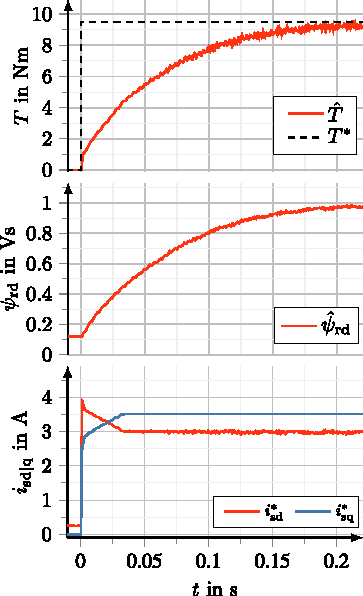
\includegraphics[height=0.8\textheight]{fig/lec04/Torque_transient_example.pdf}
				\caption{Transient torque response example}
				\label{fig:IM_transient_torque_example}
			\end{figure}
		\end{column}
	\end{columns}
\end{frame}

%%%%%%%%%%%%%%%%%%%%%%%%%%%%%%%%%%%%%%%%%%%%%%%%%%%%%%%%%%%%%
\subsubsection{Modulation degree control}
%%%%%%%%%%%%%%%%%%%%%%%%%%%%%%%%%%%%%%%%%%%%%%%%%%%%%%%%%%%%%

%%%%%%%%%%%%%%%%%%%%%%%%%%%%%%%%%%%%%%%%%%%%%%%%%%%%%%%%%%%%%%%
%% Modulation degree control structure %%
%%%%%%%%%%%%%%%%%%%%%%%%%%%%%%%%%%%%%%%%%%%%%%%%%%%%%%%%%%%%%%%%

\begin{frame}
	\frametitle{Modulation degree control structure}
	\centering
	\begin{figure}
		\begin{circuitikz}[>=Latex, scale=0.75, transform shape]
			\tikzset{
				detailblock/.style = {ctrlblock, align=center, minimum width=1.34cm, minimum height=1.02cm, font=\small},
				intblock/.style = {ctrlblock, align=center, minimum width=1.10cm, minimum height=1.02cm, font=\small},
				tfblock/.style = {draw, rectangle, thick, minimum width=2.00cm, minimum height=1.90cm, inner sep=0pt},
				dublock/.style = {ctrlblock, align=center, minimum width=1.72cm, minimum height=1.48cm, font=\small},
				satblock/.style = {draw, rectangle, thick, minimum width=1.64cm, minimum height=1.98cm, inner sep=0pt},
				sig/.style = {font=\small, inner sep=1.5pt},
				tap/.style = {circle, fill=black, inner sep=1.15pt}
			}
			\ctikzset{block left anchors pos=0.7, block right anchors pos=0.7}
			\def\phaseport{0.72}
			\def\smallgap{0.6cm}
			\def\medgap{1.0cm}
			\def\biggap{2.25cm}

			\node[signedmixer, tripoles/signedmixer/west={$+$}, tripoles/signedmixer/south={$-$}] (sumd) {};

			\coordinate[left=\smallgap of sumd] (refd);
			\draw[->, thick] (refd) -- (sumd.west);
			\node[sig, above] at ($(refd)!0.1!(sumd.west)$) {$m^{*}$};

			\coordinate[below=\biggap*0.8 of sumd.south] (fbd);
			\draw[->, thick] (fbd) -- (fbd |- sumd.south);
			\node[sig, left] at ($(fbd)!0.10!(fbd |- sumd.south)$) {$m$};


			\node[detailblock, right=\smallgap of sumd] (kpd) {PI + ARW};

			\draw[->, thick] (sumd) -- (kpd);

			\node[saturationshape, right=\smallgap of kpd] (saturation) {};
			\draw[->, thick] (kpd.east) -- (saturation.left);

			\draw[thick, ->] (saturation.right) -- node[sig, pos=0.4, below, yshift=-1mm]{$\Delta \psi_\mathrm{r}$} ++(\medgap, 0) coordinate (out_delta_psi);

			\node[signedmixer, tripoles/signedmixer/west={$+$}, tripoles/signedmixer/north={$+$}, anchor=west] (sumpsi) at (out_delta_psi){};
			\coordinate[above=\smallgap of sumpsi.north] (fbpsi);
			\draw[->, thick] (fbpsi) -- (fbpsi |- sumpsi.north);
			\node[sig, right, anchor=west] at ($(fbpsi)!0.10!(fbpsi |- sumpsi.north)$) {$\psi'_{\mathrm{r,max}}$};



			\node[detailblock, right=\medgap of sumpsi] (OPS) {OPS};
			\node[detailblock, right=\medgap of OPS] (fluxctrl) {Flux\\controller};
			\node[signedmixer, tripoles/signedmixer/west={$+$}, tripoles/signedmixer/north={$-$}, right=\medgap of fluxctrl] (sumcc) {};
			\draw[->, thick] (fluxctrl.east) -- node[sig, below, yshift=-1mm]{$\bm{i}^*_{\mathrm{s,dq}}$} (sumcc.west);

			\draw[->, thick] (sumpsi.east) --node[sig, below, yshift=-1mm]{$\psi_\mathrm{r,max}$} (OPS.west);
			\draw[->, thick] (OPS.east) -- node[sig, below, yshift=-1mm]{$\bm{\psi}^*_{\mathrm{r,lim}}$} (fluxctrl.west);
			\draw[->, thick] (OPS.east) -- node[sig, above, yshift=1mm]{$T_{\mathrm{lim}}^*$} (fluxctrl.west);

			\node[detailblock, right=\medgap of sumcc] (CC) {Current\\ controller};
			\draw[->, thick] (sumcc.east) -- (CC.west);
			\node[detailblock, right=\smallgap of CC] (MA) {Machine};
			\draw[->, thick] (CC.east) -- (MA.west);
			\draw[->,thick] (MA.east) -- node[sig, pos=0.4, below]{$\bm{i}_{\mathrm{s,dq}}$} ++(\medgap, 0) coordinate (out_idq);
			\coordinate (out_feedback_back) at ($(out_idq)!0.5!(out_idq -| MA.east)$);
			\draw[->, thick] (MA.east) -- (out_feedback_back) to [short, *-] ($(out_feedback_back)+(0, 1.5cm)$) -| (sumcc.north);
			\node[signedmixer, tripoles/signedmixer/east={$*$}, tripoles/signedmixer/north={$/$}] (summ) at (fbd -| sumpsi.north){};
			\coordinate[above=\smallgap of summ.north] (fbudc);
			\draw[->, thick] (fbudc) -- (fbudc |- summ.north);
			\node[sig, right, anchor=west] at ($(fbudc)!0.10!(fbudc |- summ.north)$) {$\nicefrac{u_{\mathrm{dc}}}{\sqrt{3}}$};
			\node[detailblock, left=\medgap of summ] (abs) {$||\bm{x}||_2$};
			\draw[->, thick] ($(CC.east)!0.25!(MA.west)$) to [short, *-] ($(CC.east)!0.25!(MA.west)$) |- node[sig, left, yshift=2mm, xshift=-1mm]{$\bm{u}^*_{\mathrm{s,dq}}$} (summ.east);
			\draw[->, thick] (summ.west) -- (abs.east);
			\draw[->, thick] (abs.west) -| (sumd.south);

		\end{circuitikz}%
		\caption{Modulation degree controller  (inner PI + ARW loop is structurally identical to PMSM case from \figref{fig:modulation_degree_control} and is not shown here due to space reasons).}
		\label{fig:modulation_degree_control_IM}
	\end{figure}\pause%
	\vspace{-0.65cm}
	\begin{varblock}{Remark}
		In contrast to the PMSM case, the closed-loop rotor flux dynamics are mostly dominant for the IM drive. While the above structure focuses on manipulating $\psi_\mathrm{r}$ according to a rotor-flux-oriented FOC approach, the same can be applied to a stator-flux-oriented FOC (or any other controller) concept by replacing $\psi_\mathrm{r}$ with $\psi_\mathrm{s}$.
	\end{varblock}
\end{frame}

%%%%%%%%%%%%%%%%%%%%%%%%%%%%%%%%%%%%%%%%%%%%%%%%%%%%%%%%%%%%%%%
%% Two command-variable views %%
%%%%%%%%%%%%%%%%%%%%%%%%%%%%%%%%%%%%%%%%%%%%%%%%%%%%%%%%%%%%%%%%
\begin{frame}
	\frametitle{IM modulation controller: command-variable choice}
	The modulation controller regulates the voltage utilization via the modulation index:
	\begin{equation}
		m[k]=\sqrt{3}\frac{\left\|\bm{u}^{\psi_{\mathrm r},*}_{\mathrm{s,dq}}[k]\right\|_2}{u_{\mathrm{dc}}[k]},
		\qquad e_m[k]=m^*[k]-m[k].
		\label{eq:IM_mod_v06_m_definition}
	\end{equation}\pause%
	Since $\bm{u}^{\psi_{\mathrm r},*}_{\mathrm{s,dq}}[k]\approx \omega_{\psi_{\mathrm r}}\bm{\psi}_{\mathrm{s,dq}}^{\psi_{\mathrm r}}$, a classical flux-weakening interpretation would let the controller manipulate a stator-flux limit,
	\begin{equation}
		\psi_{\mathrm{s,max}}=\psi'_{\mathrm{s,max}}+\Delta\psi_{\mathrm{s,max}},
		\qquad
		\psi'_{\mathrm{s,max}}=\frac{u_{\mathrm{dc}}}{\sqrt{3}|\omega_{\psi_{\mathrm r}}|} .
		\label{eq:IM_mod_v06_classical_stator_limit}
	\end{equation}\pause%
	In an IM rotor-flux-oriented FOC, however, the OPS and flux controller do not manipulate $\psi_{\mathrm{s}}$ directly. \pause  Their controlled variable is
	\begin{equation}
		\psi_{\mathrm{r,d}}^{\psi_{\mathrm r},*},
		\qquad
		\psi_{\mathrm{r,max}}^{\psi_{\mathrm r},*}=\psi_{\mathrm{r,max}}^{\prime}+\Delta\psi_{\mathrm{r,max}}^{\psi_{\mathrm r},*} .
		\label{eq:IM_mod_v06_actual_rotor_limit}
	\end{equation}\pause%
	Therefore the IM modulation controller must be derived once in the classical stator-flux view and then transformed to the actually implemented rotor-flux command.
\end{frame}

%%%%%%%%%%%%%%%%%%%%%%%%%%%%%%%%%%%%%%%%%%%%%%%%%%%%%%%%%%%%%%%
%% Classical PMSM-like view %%
%%%%%%%%%%%%%%%%%%%%%%%%%%%%%%%%%%%%%%%%%%%%%%%%%%%%%%%%%%%%%%%
\begin{frame}
	\frametitle{Classical stator-flux modulation-controller view}
	From
	\begin{equation*}
		\bm{u}_{\mathrm{s,dq}}^{\psi_{\mathrm r}}
		=R_{\mathrm{s}}\bm{i}_{\mathrm{s,dq}}^{\psi_{\mathrm r}}
		+\frac{\mathrm{d}}{\mathrm{d}t}\bm{\psi}_{\mathrm{s,dq}}^{\psi_{\mathrm r}}
		+\omega_{\psi_{\mathrm r}}\bm{J}\bm{\psi}_{\mathrm{s,dq}}^{\psi_{\mathrm r}}
	\end{equation*}\pause%
	the stator voltage demand during steady state is (neglecting the ohmic voltage drop)
	\begin{equation}
		\left\|\bm{u}_{\mathrm{s,dq}}^{\psi_{\mathrm r}}\right\|_2
		\approx |\omega_{\psi_{\mathrm r}}|\left\|\bm{\psi}_{\mathrm{s,dq}}^{\psi_{\mathrm r}}\right\|_2 .
		\label{eq:IM_mod_v06_voltage_flux_approx}
	\end{equation}\pause%
	If $\Delta\psi_{\mathrm{s,max}}$ were the controller output and the stator-flux realization were summarized by $G_{\psi_{\mathrm{s}}}(\mathrm{z})$, the classical SISO plant would be
	\begin{equation}
		G_{\mathrm{p},m}^{\psi_{\mathrm{s}}}(\mathrm{z})
		=\frac{\Delta M(\mathrm{z})}{\Delta\Psi_{\mathrm{s,max}}(\mathrm{z})}
		\approx
		K_mG_{\psi_{\mathrm{s}}}(\mathrm{z}),
		\qquad
		K_m=\frac{\sqrt{3}|\omega_{\psi_{\mathrm r}}|}{u_{\mathrm{dc}}} .
		\label{eq:IM_mod_v06_classical_siso}
	\end{equation}
\end{frame}


%%%%%%%%%%%%%%%%%%%%%%%%%%%%%%%%%%%%%%%%%%%%%%%%%%%%%%%%%%%%%%%
%% Linear model mapping %%
%%%%%%%%%%%%%%%%%%%%%%%%%%%%%%%%%%%%%%%%%%%%%%%%%%%%%%%%%%%%%%%

\begin{frame}
	\frametitle{Magnetic model: stator-to-rotor flux mapping}
	For the usual apparent inductance definitions and fixed requested torque $T^*$, we have
	\begin{equation}
		\begin{gathered}
			\psi_{\mathrm{s,d}}^{\psi_{\mathrm r}}=a_\psi\psi_{\mathrm r},
			\qquad
			\psi_{\mathrm{s,q}}^{\psi_{\mathrm r}}=\sigma L_{\mathrm{s,app}}\frac{T^*}{c_T\psi_{\mathrm r}},
			\qquad
			a_\psi=\frac{L_{\mathrm{s,app}}}{L_{\mathrm{m,app}}},
			\quad
			c_T=\frac{3}{2}p\frac{L_{\mathrm{m,app}}}{L_{\mathrm{r,app}}}.
		\end{gathered}
		\label{eq:IM_mod_v06_linear_flux_components}
	\end{equation}\pause%
	With the flux ratio
	\begin{equation}
		\kappa_\psi
		=\frac{\psi_{\mathrm{s,q}}^{\psi_{\mathrm r}}}{\psi_{\mathrm{s,d}}^{\psi_{\mathrm r}}}
		=\frac{\sigma L_{\mathrm{m,app}}T^*}{c_T\psi_{\mathrm r}^{2}},
		\label{eq:IM_mod_v06_kappa_def}
	\end{equation}\pause%
	the modulation-relevant stator-flux magnitude is
	\begin{equation}
		\psi_{\mathrm{s}}(\psi_{\mathrm r},T^*)
		=\left\|\bm{\psi}_{\mathrm{s,dq}}^{\psi_{\mathrm r}}\right\|_2
		=a_\psi\psi_{\mathrm r}\sqrt{1+\kappa_\psi^2} .
		\label{eq:IM_mod_v06_linear_psis_map}
	\end{equation}\pause%
	Hence, the \hl{stator-rotor-flux sensitivity} is
	\begin{equation}
		K_{\psi_{\mathrm{s}}\psi_{\mathrm r}}
		=\left.\frac{\partial\psi_{\mathrm{s}}}{\partial\psi_{\mathrm r}}\right|_{T^*}
		=a_\psi\frac{1-\kappa_\psi^2}{\sqrt{1+\kappa_\psi^2}}
		\stackrel{|\kappa_\psi|\ll 1}{\approx} \frac{L_{\mathrm{s,app}}}{L_{\mathrm{m,app}}} .
		\label{eq:IM_mod_v06_linear_sensitivity}
	\end{equation}
\end{frame}


%%%%%%%%%%%%%%%%%%%%%%%%%%%%%%%%%%%%%%%%%%%%%%%%%%%%%%%%%%%%%%%
%% Plant modeling for a rotor-flux-limit command %%
%%%%%%%%%%%%%%%%%%%%%%%%%%%%%%%%%%%%%%%%%%%%%%%%%%%%%%%%%%%%%%%
\begin{frame}
	\frametitle{Plant modeling for a rotor-flux-limit command}
	The local \hl{small-signal chain} based on the controller structure from \figref{fig:modulation_degree_control_IM} is
	\begin{equation}
		\Delta\psi_{\mathrm{r,d,max}}^{*}
		\xrightarrow{K_{\mathrm{OPS}}}
		\Delta\psi_{\mathrm{r}}^{\psi_{\mathrm r},*}
		\xrightarrow{G_{\psi}(\mathrm{z})}
		\Delta\psi_{\mathrm{r}}^{\psi_{\mathrm r}}
		\xrightarrow{K_{\psi_{\mathrm{s}}\psi_{\mathrm r}}}
		\Delta\left\|\bm{\psi}_{\mathrm{s,dq}}^{\psi_{\mathrm r}}\right\|_2
		\xrightarrow{K_m}
		\Delta m .
		\label{eq:IM_mod_v06_actual_chain}
	\end{equation}\pause%
	Assuming that the flux-limiting branch of the OPS is active, it holds:
	\begin{equation}
		K_{\mathrm{OPS}}=\frac{\partial\psi_{\mathrm{r}}^{\psi_{\mathrm r},*}}{\partial\psi_{\mathrm{r,max}}^{\psi_{\mathrm r},*}}
		\approx 1 .
		\label{eq:IM_mod_v06_kops}
	\end{equation}\pause%
	From \eqref{eq:closed_loop_TF_rotor_flux_IM}, the rotor-flux controller design yields the closed-loop transfer function
	\[
		G_{\psi}(z)
		=
		\frac{\Psi_{\mathrm{r,d}}(z)}{\Psi_{\mathrm{r,d}}^*(z)}
		=
		\frac{
			b_\psi\left[(K_{\mathrm p,\psi}+K_{\mathrm i,\psi}T_{\mathrm s})z-K_{\mathrm p,\psi}\right]
		}{
			z^2-S_\psi z+P_\psi
		} .
	\]
\end{frame}

%%%%%%%%%%%%%%%%%%%%%%%%%%%%%%%%%%%%%%%%%%%%%%%%%%%%%%%%%%%%%%%
%% Plant modeling for a rotor-flux-limit command (cont.) %%
%%%%%%%%%%%%%%%%%%%%%%%%%%%%%%%%%%%%%%%%%%%%%%%%%%%%%%%%%%%%%%%
\begin{frame}
	\frametitle{Plant modeling for a rotor-flux-limit command (cont.)}
	With the practical choice \(p_1=p_2=\lambda_\psi\), i.e.
	\(S_\psi=2\lambda_\psi\), \(P_\psi=\lambda_\psi^2\), and the pole-placement gains from the rotor-flux-control design,
	\[
		G_{\psi}(z)
		=
		\frac{
			(a_\psi+1-2\lambda_\psi)z+\lambda_\psi^2-a_\psi
		}{
			(z-\lambda_\psi)^2
		} .
	\]\pause%
	For \hl{reduced (easier) modulation-controller design}, approximate it by a unity-gain PT1 model
	\begin{equation}
		G'_{\psi}(z)
		=
		\frac{1-\lambda'_{\psi}}{z-\lambda'_{\psi}},
		\qquad
		G'_{\psi}(1)=1 .
	\end{equation}\pause%
	A low-frequency moment-matched choice is obtained from
	\begin{equation}
		\left.
		\frac{\mathrm d G'_{\psi}(z)}{\mathrm d z}
		\right|_{z=1}
		=
		\left.
		\frac{\mathrm d G_{\psi}(z)}{\mathrm d z}
		\right|_{z=1},
	\end{equation}\pause%
	which gives the reduced pole matching formula
	\begin{equation}
		\lambda'_{\psi}
		=
		1-
		\frac{(1-\lambda_\psi)^2}{1-a_\psi}.
	\end{equation}
\end{frame}

%%%%%%%%%%%%%%%%%%%%%%%%%%%%%%%%%%%%%%%%%%%%%%%%%%%%%%%%%%%%%%%
%% Time-scale argument %%
%%%%%%%%%%%%%%%%%%%%%%%%%%%%%%%%%%%%%%%%%%%%%%%%%%%%%%%%%%%%%%%
\begin{frame}
	\frametitle{Dominant dynamics of the IM modulation plant}
	The current controller still creates the voltage demand that is used for $m$, but its closed-loop dynamics are much faster than the rotor-flux dynamics:
	\begin{equation}
		\tau_{\mathrm{i,cl}}\ll\tau_{\psi,\mathrm{cl}},
		\qquad
		\tau_{\psi,\mathrm{cl}}\approx 10\ldots100\,\tau_{\mathrm{i,cl}} .
		\label{eq:IM_mod_v06_time_scale}
	\end{equation}\pause%
	Hence, for modulation-controller design, the current loop is treated as quasi-stationary.  The dominant plant becomes
	\begin{equation}
		G_{\mathrm{p},m}(\mathrm{z})
		=\frac{\Delta M(\mathrm{z})}{\Delta\Psi_{\mathrm{r,d,max}}^{*}(\mathrm{z})}
		\approx
		K_mK_{\psi_{\mathrm{s}}\psi_{\mathrm r}}K_{\mathrm{OPS}}G'_{\psi}(\mathrm{z}) .
		\label{eq:IM_mod_v06_flux_dominant_plant}
	\end{equation}\pause%
	With $K_{\mathrm{OPS}}\approx1$, find
	\begin{equation}
		G_{\mathrm{p},m}(\mathrm{z})
		\approx K_mK_{\psi_{\mathrm{s}}\psi_{\mathrm r}}\frac{1-\lambda'_{\psi}}{\mathrm{z}-\lambda'_{\psi}} .
		\label{eq:IM_mod_v06_reduced_rotor_plant}
	\end{equation}
\end{frame}

%%%%%%%%%%%%%%%%%%%%%%%%%%%%%%%%%%%%%%%%%%%%%%%%%%%%%%%%%%%%%%%
%% Direct plant comparison %%
%%%%%%%%%%%%%%%%%%%%%%%%%%%%%%%%%%%%%%%%%%%%%%%%%%%%%%%%%%%%%%%
\begin{frame}
	\frametitle{Plant models: stator- vs. rotor-flux manipulation}
	Both variants share the voltage-to-flux gain and the dominant rotor-flux dynamics,
	\begin{equation}
		K_m=\sqrt{3}\frac{|\omega_{\psi_{\mathrm r}}|}{u_{\mathrm{dc}}},
		\qquad
		G_{\psi}(\mathrm{z})\approx\frac{1-\lambda'_{\psi}}{\mathrm{z}-\lambda'_{\psi}} .
		\label{eq:IM_mod_v06_common_parts}
	\end{equation}\pause%
	The difference is the command domain before the rotor-flux controller:
	\begin{equation}
		\begin{array}{rclcl}
			\Delta\Psi_{\mathrm{s,max}}
			 & \xrightarrow{\;K_{\psi_{\mathrm r}\psi_{\mathrm{s}}}\;}                                         &
			\Delta\Psi_{\mathrm{r,max}}^{*}
			 & \xrightarrow{\;K_{\mathrm{OPS}}G'_{\psi}(\mathrm{z})K_{\psi_{\mathrm{s}}\psi_{\mathrm r}}K_m\;} &
			\Delta M,                                                                                            \\[1mm]
			\Delta\Psi_{\mathrm{r,d,max}}^{*}
			 &                                                                                                 &
			\Delta\Psi_{\mathrm{r,max}}^{*}
			 & \xrightarrow{\;K_{\mathrm{OPS}}G'_{\psi}(\mathrm{z})K_{\psi_{\mathrm{s}}\psi_{\mathrm r}}K_m\;} &
			\Delta M.
		\end{array}
		\label{eq:IM_mod_v06_plant_chains_compact}
	\end{equation}\pause%
	Hence, the two SISO plants are
	\begin{equation}
		\begin{aligned}
			G_{\mathrm{p},m}^{\psi_{\mathrm s}}(\mathrm{z})
			 & =\frac{\Delta M}{\Delta\Psi_{\mathrm{s,max}}}
			\approx K_mK_{\psi_{\mathrm{s}}\psi_{\mathrm r}}K_{\mathrm{OPS}}G'_{\psi}(\mathrm{z})K_{\psi_{\mathrm r}\psi_{\mathrm{s}}}
			\approx K_mG'_{\psi}(\mathrm{z}),                      \\[1mm]\pause%
			G_{\mathrm{p},m}^{\psi_{\mathrm r}}(\mathrm{z})
			 & =\frac{\Delta M}{\Delta\Psi_{\mathrm{r,d,max}}^{*}}
			\approx K_mK_{\psi_{\mathrm{s}}\psi_{\mathrm r}}K_{\mathrm{OPS}}G'_{\psi}(\mathrm{z}).
		\end{aligned}
		\label{eq:IM_mod_v06_plant_models_compact}
	\end{equation}\pause%
	\begin{equation}
		\boxed{\text{same dynamics }G'_{\psi}(\mathrm{z})}
		\qquad
		\boxed{\vphantom{G'}\text{different gain for IM output: }K_{\psi_{\mathrm{s}}\psi_{\mathrm r}}}
	\end{equation}
\end{frame}


%%%%%%%%%%%%%%%%%%%%%%%%%%%%%%%%%%%%%%%%%%%%%%%%%%%%%%%%%%%%%%%
%% PI controller design %%
%%%%%%%%%%%%%%%%%%%%%%%%%%%%%%%%%%%%%%%%%%%%%%%%%%%%%%%%%%%%%%%
\begin{frame}
	\frametitle{PI design for the rotor-flux-output plant}
	The discrete-time PI controller outputs a rotor-flux-limit correction:
	\begin{equation}
		\Delta\Psi_{\mathrm{r,max}}^{*}(\mathrm{z})
		=G_{\mathrm{c},m}(\mathrm{z})E_m(\mathrm{z}),
		\qquad
		G_{\mathrm{c},m}(\mathrm{z})
		=K_{\mathrm{p},m}+K_{\mathrm{i},m}T_{\mathrm{s}}\frac{\mathrm{z}}{\mathrm{z}-1} .
		\label{eq:IM_mod_v06_PI_rotor_output}
	\end{equation}\pause%
	Using
	\begin{equation}
		G_{\mathrm{p},m}(\mathrm{z})
		\approx\frac{b_m}{\mathrm{z}-a_m},
		\qquad
		a_m=\lambda'_{\psi},
		\qquad
		b_m=K_mK_{\psi_{\mathrm{s}}\psi_{\mathrm r}}(1-\lambda'_{\psi}) .
		\label{eq:IM_mod_v06_PT1_for_design}
	\end{equation}\pause%
	The closed-loop characteristic polynomial is
	\begin{equation}
		(\mathrm{z}-1)(\mathrm{z}-a_m)+b_mK_{\mathrm{p},m}(\mathrm{z}-1)+b_mK_{\mathrm{i},m}T_{\mathrm{s}}\mathrm{z}=0 .
		\label{eq:IM_mod_v06_char_poly}
	\end{equation}
	\hl{This is the same PT1-plant design problem as before} (PMSM case), but with a different plant gain.
\end{frame}

%%%%%%%%%%%%%%%%%%%%%%%%%%%%%%%%%%%%%%%%%%%%%%%%%%%%%%%%%%%%%%%
%% Pole placement %%
%%%%%%%%%%%%%%%%%%%%%%%%%%%%%%%%%%%%%%%%%%%%%%%%%%%%%%%%%%%%%%%
\begin{frame}
	\frametitle{Pole-placement formulas and scheduling}
	With desired poles $p_1,p_2$,
	\begin{equation}
		(\mathrm{z}-p_1)(\mathrm{z}-p_2)=\mathrm{z}^2-S_m\mathrm{z}+P_m,
		\qquad
		S_m=p_1+p_2,
		\quad P_m=p_1p_2 .
		\label{eq:IM_mod_v06_desired_poly}
	\end{equation}\pause%
	Coefficient comparison gives the standard discrete PI gains
	\begin{equation}
		K_{\mathrm{p},m}=\frac{a_m-P_m}{b_m},
		\qquad
		K_{\mathrm{i},m}=\frac{1-S_m+P_m}{b_mT_{\mathrm{s}}} .
		\label{eq:IM_mod_v06_PI_gains}
	\end{equation}\pause%
	For the IM implementation use
	\begin{equation}
		b_m=\sqrt{3}\frac{|\omega_{\psi_{\mathrm r}}|}{u_{\mathrm{dc}}}
		K_{\psi_{\mathrm{s}}\psi_{\mathrm r}}(1-\lambda'_{\psi}) .
		\label{eq:IM_mod_v06_scheduled_b}
	\end{equation}\pause%
	Thus, $K_{\mathrm{p},m}$ and $K_{\mathrm{i},m}$ should be scheduled over $(T^*,\psi_{\mathrm{r,d}}^{\psi_{\mathrm r},*},\omega_{\psi_{\mathrm r}},u_{\mathrm{dc}})$ or designed conservatively for the smallest relevant $|b_m|$. As a rule of the thumb, choose $p_1=p_2=[3,\ldots,10]\cdot\lambda'_\psi$ for a sufficiently fast (but not too fast) modulation controller.
\end{frame}

%%%%%%%%%%%%%%%%%%%%%%%%%%%%%%%%%%%%%%%%%%%%%%%%%%%%%%%%%%%%%%%
%% Limits and anti-reset windup %%
%%%%%%%%%%%%%%%%%%%%%%%%%%%%%%%%%%%%%%%%%%%%%%%%%%%%%%%%%%%%%%%
\begin{frame}
	\frametitle{Rotor-flux limits and ARW}
	Since the controller output is a rotor-flux correction, saturation is applied in the rotor-flux domain:
	\begin{equation}
		\Delta\psi_{\mathrm{r,max}}[k]
		=\mathrm{lim}_{\Delta\psi_{\mathrm{r,min}}}^{\Delta\psi_{\mathrm{r,max}}}
		\left\{\Delta\psi_{\mathrm{r,max}}^{*}[k]\right\} .
		\label{eq:IM_mod_v06_rotor_saturation}
	\end{equation}\pause%
	Anti-reset windup is identical in structure to the PMSM case, but with the rotor-flux-domain saturation error:
	\begin{equation}
		\Delta u[k]=\Delta\psi_{\mathrm{r,max}}^{*}[k]-\Delta\psi_{\mathrm{r,max}}[k],
		\qquad
		x_{\mathrm{i},m}[k]=x_{\mathrm{i},m}^{+}[k]-\frac{K_{\mathrm{aw},m}}{K_{\mathrm{i},m}}\Delta u[k] .
		\label{eq:IM_mod_v06_ARW}
	\end{equation}\pause%
	Hence, the choice of $K_{\mathrm{aw},m}$ can follow the same route as in the PMSM case.
\end{frame}

%%%%%%%%%%%%%%%%%%%%%%%%%%%%%%%%%%%%%%%%%%%%%%%%%%%%%%%%%%%%%%%%%%
\subsection{Direct torque control}
%%%%%%%%%%%%%%%%%%%%%%%%%%%%%%%%%%%%%%%%%%%%%%%%%%%%%%%%%%%%%%%%%%

%%%%%%%%%%%%%%%%%%%%%%%%%%%%%%%%%%%%%%%%%%%%%%%%%%%%%%%%%%%%%%
%% Local TikZ block component for the IM-DTC torque loop %%
%%%%%%%%%%%%%%%%%%%%%%%%%%%%%%%%%%%%%%%%%%%%%%%%%%%%%%%%%%%%%%


%%%%%%%%%%%%%%%%%%%%%%%%%%%%%%%%%%%%%%%%%%%%%%%%%%%%%%%%%%%%%%
%% Direct torque control: high-level overview %%
%%%%%%%%%%%%%%%%%%%%%%%%%%%%%%%%%%%%%%%%%%%%%%%%%%%%%%%%%%%%%%
\begin{frame}
	\frametitle{Direct torque control (DTC) for IM drives: high-level overview}
	\centering
	\begin{figure}
		\begin{circuitikz}[x=1cm, y=1cm, scale=0.91, transform shape, >=Latex]
			\def\dtcblockheight{1.5cm}
			\def\dtcblockgaplarge{1.20cm}
			\pgfmathsetmacro{\dtcconverterscale}{\dtcblockheight/(1.4cm*0.7)}
			\tikzset{
				dtcblock/.style = {
						ctrlblock,
						align = center,
						inner sep = 3pt,
						minimum height = \dtcblockheight,
						font = \small
					},
				siglabel/.style = {font = \small, inner sep = 2pt}
			}
			\node[signedmixer, tripoles/signedmixer/west={$+$}, tripoles/signedmixer/south={$-$}] (sumT) {};
			\node[left=1.25cm of sumT] (T0) {};
			\draw[thick, ->] (T0) -- node[above, at start, anchor = south west] {$T^*$} (sumT.west);
			\node[signedmixer, tripoles/signedmixer/west={$+$}, tripoles/signedmixer/south={$-$}, below right = 0.6cm and 0.75cm of sumT] (sumPsi) {};
			\node (Psi0) at (T0 |- sumPsi) {};
			\draw[thick, ->] (Psi0) -- node[above, at start, anchor = south west] {$\|\bm{\psi}_{\mathrm{s}}\|^*$} (sumPsi.west);
			\node[crossingshape, rotate=-90, name = jumpPsi, thick] at (sumPsi.west -| sumT.south) {};
			\node[twolevelhystcontrollershape, right = \dtcblockgaplarge of sumPsi] (hyst1) {};
			\node[threelevelhystcontrollershape] at (hyst1.north |- sumT.east) (hyst2) {};
			\draw[thick, ->] (sumT.east) -- node[above, near start]{$\Delta T$} (hyst2.west);
			\draw[thick, ->] (sumPsi.east) -- node[above]{$\Delta\|\bm{\psi}_{\mathrm{s}}\|$} (hyst1.west);
			\node[dtcblock, minimum width = 2.0cm, minimum height = 3.3cm, right = \dtcblockgaplarge of hyst2.north east, anchor = north west, align = center] (swTab) {Switching\\table};
			\node[dtcblock, minimum width = 2.0cm, minimum height = 3.3cm, below = 0.5cm of swTab, align = center] (Est) {Torque \\ \& \\ flux \\ estimator};
			\draw[thick, ->] (hyst2.east)  -- ($(hyst2.east -| swTab.west)$);
			\draw[thick, ->] (hyst1.east)  -- ($(hyst1.east -| swTab.west)$);

			\node[tdcacshape, right = 2*\dtcblockgaplarge of swTab.north east, anchor = north west,circuitikz/blocks/scale = \dtcconverterscale]  (conv) {};
			\node[threephasemotorshaftshape, below = 3 cm of conv.south, anchor = center, circuitikz/blocks/scale = \dtcconverterscale
			] (motor) {};

			\draw[thick] (conv.south) to[currtap, name=ctdc] (motor.north);
			\coordinate (ctdcQuarterTop) at ($(conv.south)+(0.5,0)$);
			\path[name path = motorcircle] (motor.center) circle[radius = \dimexpr\dtcblockheight/2\relax];
			\path[name path = ctdcQuarterLine] (ctdcQuarterTop) -- ($(ctdcQuarterTop |- motor.south)+(0,-0.2)$);
			\path[name intersections = {of = motorcircle and ctdcQuarterLine, by = ctdcQuarterBottom}];
			\coordinate (ctdcQuarterTapTop) at ($(ctdcQuarterTop)!0.05!(ctdcQuarterBottom)$);
			\coordinate (ctdcQuarterTapBottom) at ($(ctdcQuarterTop)!0.4!(ctdcQuarterBottom)$);
			\draw[thick](ctdcQuarterTop) -- (ctdcQuarterTapTop);
			\draw[thick] (ctdcQuarterTapTop) to[currtap, name=ctdcquarter] (ctdcQuarterTapBottom);
			\draw[thick] (ctdcQuarterTapBottom) -- (ctdcQuarterBottom);
			\coordinate (ctdcQuarterLeftTop) at ($(conv.south)+(-0.5,0)$);
			\path[name path = ctdcQuarterLeftLine] (ctdcQuarterLeftTop) -- ($(ctdcQuarterLeftTop |- motor.south)+(0,-0.2)$);
			\path[name intersections = {of = motorcircle and ctdcQuarterLeftLine, by = ctdcQuarterLeftBottom}];
			\coordinate (ctdcQuarterLeftTapTop) at ($(ctdcQuarterLeftTop)!0.525!(ctdcQuarterLeftBottom)$);
			\coordinate (ctdcQuarterLeftTapBottom) at ($(ctdcQuarterLeftTop)!0.875!(ctdcQuarterLeftBottom)$);
			\draw[thick] (ctdcQuarterLeftTop) -- (ctdcQuarterLeftTapTop);
			\draw[thick] (ctdcQuarterLeftTapTop) to[currtap, name=ctdcquarterleft] (ctdcQuarterLeftTapBottom);
			\draw[thick] (ctdcQuarterLeftTapBottom) -- (ctdcQuarterLeftBottom);

			\coordinate (dtcVoltSenseInA) at ($(Est.north  east)!0.125!(Est.south east)$);
			\coordinate (dtcVoltSenseInB) at ($(Est.north  east)!0.25!(Est.south east)$);
			\coordinate (dtcVoltSenseInC) at ($(Est.north  east)!0.375!(Est.south east)$);
			\coordinate (dtcCurrSenseInA) at ($(Est.north  east)!0.5!(Est.south east)$);
			\coordinate (dtcCurrSenseInB) at ($(Est.north  east)!0.625!(Est.south east)$);
			\coordinate (dtcCurrSenseInC) at ($(Est.north  east)!0.75!(Est.south east)$);
			\coordinate (dtcMotorSense) at ($(Est.north  east)!0.875!(Est.south east)$);


			\coordinate (VoltSenseCEdge) at ($(swTab.north east)!0.429!(conv.north west)$);
			\coordinate (VoltSenseBEdge) at ($(swTab.north east)!0.286!(conv.north west)$);
			\coordinate (VoltSenseAEdge) at ($(swTab.north east)!0.143!(conv.north west)$);
			\coordinate (CurrSenseAEdge) at ($(swTab.north east)!0.571!(conv.north west)$);
			\coordinate (CurrSenseBEdge) at ($(swTab.north east)!0.714!(conv.north west)$);
			\coordinate (CurrSenseCEdge) at ($(swTab.north east)!0.857!(conv.north west)$);

			\node[crossingshape, name = jumpiB, thick] at (ctdcquarter.tap -| conv.south) {};
			\node[crossingshape, name = jumpiC, thick] at (ctdcquarter.tap -| ctdcQuarterLeftTop) {};
			\node[crossingshape, name = jumpiC2, thick] at (ctdc.tap -| ctdcQuarterLeftTop) {};

			\draw[thick] (ctdcquarter.tap) -- (jumpiB.east);
			\draw[thick] (jumpiB.west) -- (jumpiC.east);
			\draw[thick, ->] (jumpiC.west) -| node[above, near end ] {$i_\mathrm{a}$} ($(CurrSenseAEdge |- ctdcquarter.tap)$) |- (dtcCurrSenseInA);
			\draw[thick] (ctdc.tap) -- (jumpiC2.east);
			\draw[thick, ->] (jumpiC2.west) -| node[above, near end ] {$i_\mathrm{b}$} ($(CurrSenseBEdge |- ctdc.tap)$) |- (dtcCurrSenseInB);
			\draw[thick, ->] (ctdcquarterleft.tap) -| node[above, near end ] {$i_\mathrm{c}$} ($(CurrSenseCEdge |- ctdcquarterleft.tap)$) |- (dtcCurrSenseInC);

			\draw[thick, ->] (motor.south) |- node[above left] {$\omega$} (dtcMotorSense);

			\coordinate (swTabOut) at ($(swTab.east |- conv.west)$);

			\foreach \dy/\phase in {0.5/a, 0.00/b, -0.5/c} {
					\draw[thick, ->] ($(swTabOut)+(0,\dy)$) -- ($(conv.west)+(0,\dy)$) coordinate (convS\phase);
					\node[siglabel, above] at ($($(swTabOut)+(0,\dy)$)!0.5!($(conv.west)+(0,\dy)$)$) {$s_\mathrm{\phase}$};
				}
			\coordinate (TorqueEstOut) at ($(Est.north  west)!0.75!(Est.south west)$);
			\coordinate (FluxEstOut) at ($(Est.north  west)!0.5!(Est.south west)$);
			\coordinate (AuxEstOut) at ($(Est.north  west)!0.25!(Est.south west)$);
			\coordinate (AuxSwIn) at ($(swTab.north  west)!0.85!(swTab.south west)$);

			\draw[thick] (TorqueEstOut)  -| node[at start, anchor = south east] {$\hat{T}$} (jumpPsi.east);
			\draw[thick, ->] (jumpPsi.west) -- (sumT.south);
			\draw[thick, ->] (FluxEstOut)  -| node[at start, anchor = south east] {$\|\hat{\bm{\psi}}_{\mathrm{s}}\|$} (sumPsi.south);
			\draw[thick, ->] (AuxEstOut)   -- node[at start, anchor = south east] {$\omega, \hat{\bm{\psi}}_{\mathrm{s},\upalpha\upbeta}$} ($(AuxEstOut -| hyst1.south)$) |-   (AuxSwIn);

			\node[crossingshape, rotate=-90, name = jumpSb, thick] at (convSb -| VoltSenseAEdge) {};
			\node[crossingshape, rotate=-90, name = jumpSc, thick] at (convSc -| VoltSenseAEdge) {};
			\node[crossingshape, rotate=-90, name = jumpSc2, thick] at (convSc -| VoltSenseBEdge) {};

			\draw[thick] ($(VoltSenseAEdge |- convSa)$) to [short, *-] (jumpSb.west);
			\draw[thick] (jumpSb.east) -- (jumpSc.west);
			\draw[thick, ->] (jumpSc.east) |- (dtcVoltSenseInA);
			\draw[thick] ($(VoltSenseBEdge |- convSb)$) to [short, *-] (jumpSc2.west);
			\draw[thick, ->] (jumpSc2.east) |- (dtcVoltSenseInB);
			\draw[thick, ->] ($(VoltSenseCEdge |- convSc)$) to [short, *-] ($(VoltSenseCEdge |- convSc)$) |- (dtcVoltSenseInC);
		\end{circuitikz}
		\caption{Overview of a direct torque control system for IM drives (not considering superimposed OPS and modulation-degree control, the DTC for PMSM and IM are structurally identical).}
		\label{fig:dtc_IM_high_level}
	\end{figure}
\end{frame}



%%%%%%%%%%%%%%%%%%%%%%%%%%%%%%%%%%%%%%%%%%%%%%%%%%%%%%%%%%%%%%
%% IM torque relation in stator-flux DTC %%
%%%%%%%%%%%%%%%%%%%%%%%%%%%%%%%%%%%%%%%%%%%%%%%%%%%%%%%%%%%%%%
\begin{frame}
	\frametitle{DTC torque mechanism for the IM}
	Expressing the stator current in terms of the stator and rotor flux linkages, we have
	\begin{equation}
		\bm{i}_{\mathrm{s},\upalpha\upbeta}
		=\frac{1}{\sigma L_\mathrm{s,app}}\left(\bm{\psi}_{\mathrm{s},\upalpha\upbeta}
		-\frac{L_\mathrm{m,app}}{L_\mathrm{r,app}}\bm{\psi}_{\mathrm{r},\upalpha\upbeta}\right).
		\label{eq:IM_DTC_stator_current_flux_relation_v2}
	\end{equation}\pause%
	The \hl{IM's torque} can be represented as the \hl{dot product of the stator and rotor flux linkages}:
	\begin{equation}
		\begin{split}
			T & = \frac{3}{2}p \bm{i}^{\T}_{\mathrm{s},\upalpha\upbeta}\bm{J}\bm{\psi}_{\mathrm{s},\upalpha\upbeta}
			= \frac{3}{2}p\frac{L_\mathrm{m,app}}{\sigma L_\mathrm{s,app}L_\mathrm{r,app}}
			\bm{\psi}_{\mathrm{s},\upalpha\upbeta}^{\T}\bm{J}\bm{\psi}_{\mathrm{r},\upalpha\upbeta}                 \\
			  & = \frac{3}{2}p\frac{L_\mathrm{m,app}}{\sigma L_\mathrm{s,app}L_\mathrm{r,app}}
			\|\bm{\psi}_\mathrm{s}\|\,\|\bm{\psi}_\mathrm{r}\|\sin(\delta).
		\end{split}
		\label{eq:IM_DTC_torque_flux_angle_v2}
	\end{equation}\pause%
	\begin{itemize}
		\item The rotor flux linkage is a comparatively slow state due to the rotor time constant.\pause%
		\item DTC therefore moves the stator flux vector directly to change both $\|\bm{\psi}_\mathrm{s}\|$ and the torque-producing angle $\delta$.
	\end{itemize}
\end{frame}

%%%%%%%%%%%%%%%%%%%%%%%%%%%%%%%%%%%%%%%%%%%%%%%%%%%%%%%%%%%%%%
%% Stator flux and torque estimation %%
%%%%%%%%%%%%%%%%%%%%%%%%%%%%%%%%%%%%%%%%%%%%%%%%%%%%%%%%%%%%%%
\begin{frame}
	\frametitle{Stator flux and torque estimation for DTC}
	In stationary coordinates, the stator voltage equation directly gives
	\begin{equation}
		\frac{\mathrm{d}}{\mathrm{d}t}\bm{\psi}_{\mathrm{s},\upalpha\upbeta}(t)
		=\bm{u}_{\mathrm{s},\upalpha\upbeta}(t)-R_\mathrm{s}\bm{i}_{\mathrm{s},\upalpha\upbeta}(t).
		\label{eq:IM_DTC_stator_flux_voltage_model_ct_v2}
	\end{equation}\pause%
	A \hl{simple discrete-time voltage-model estimator} is
	\begin{equation}
		\hat{\bm{\psi}}_{\mathrm{s},\upalpha\upbeta}[k+1]
		=\hat{\bm{\psi}}_{\mathrm{s},\upalpha\upbeta}[k]
		+T_\mathrm{s}\left(\hat{\bm{u}}_{\mathrm{s},\upalpha\upbeta}[k]-R_\mathrm{s}\bm{i}_{\mathrm{s},\upalpha\upbeta}[k]\right),
		\label{eq:IM_DTC_stator_flux_voltage_model_dt_v2}
	\end{equation}\pause%
	with the torque estimate
	\begin{equation}
		\hat{T}[k]
		=\frac{3}{2}p\,\bm{i}_{\mathrm{s},\upalpha\upbeta}^{\T}[k]
		\bm{J}\hat{\bm{\psi}}_{\mathrm{s},\upalpha\upbeta}[k].
		\label{eq:IM_DTC_torque_estimate_v2}
	\end{equation}\pause%
	\begin{itemize}
		\item $\hat{\bm{u}}_\mathrm{s}$ is typically reconstructed from $s_\mathrm{a,b,c}$, $u_\mathrm{dc}$ and an inverter model.\pause%
		\item At low stator frequencies, $R_\mathrm{s}$ errors and measurement offsets must be compensated to avoid flux-estimator drift -- or a low-pass filtered integration must be used.
	\end{itemize}
\end{frame}

%%%%%%%%%%%%%%%%%%%%%%%%%%%%%%%%%%%%%%%%%%%%%%%%%%%%%%%%%%%%%%
%% Voltage-model route to rotor flux estimation %%
%%%%%%%%%%%%%%%%%%%%%%%%%%%%%%%%%%%%%%%%%%%%%%%%%%%%%%%%%%%%%%
\begin{frame}
	\frametitle{Voltage-model route: rotor flux dynamics in $\upalpha\upbeta$}
	Starting from the flux ODEs used for the discrete-time IM model, express both flux vectors in stator-oriented $\upalpha\upbeta$ coordinates:
	\begin{equation}
		\begin{aligned}
			\frac{\mathrm{d}}{\mathrm{d}t}\hat{\bm{\psi}}^{\mathrm{s}}_{\mathrm{s},\upalpha\upbeta}
			 & =\hat{\bm{u}}^{\mathrm{s}}_{\mathrm{s},\upalpha\upbeta}
			-R_\mathrm{s}\bm{i}^{\mathrm{s}}_{\mathrm{s},\upalpha\upbeta},            \\
			\frac{\mathrm{d}}{\mathrm{d}t}\hat{\bm{\psi}}^{\mathrm{s}}_{\mathrm{r},\upalpha\upbeta}
			 & =\omega\bm{J}\hat{\bm{\psi}}^{\mathrm{s}}_{\mathrm{r},\upalpha\upbeta}
			-R_\mathrm{r}\bm{i}^{\mathrm{s}}_{\mathrm{r},\upalpha\upbeta}.
		\end{aligned}
		\label{eq:IM_DTC_flux_odes_stator_frame_v6}
	\end{equation}\pause%
	The second equation follows from $\hat{\bm{\psi}}^{\mathrm{s}}_{\mathrm{r},\upalpha\upbeta}=\bm{T}_\mathrm{p}(\varepsilon)\hat{\bm{\psi}}^{\mathrm{r}}_{\mathrm{r},\upalpha\upbeta}$ and $\frac{\mathrm{d}}{\mathrm{d}t}\hat{\bm{\psi}}^{\mathrm{r}}_{\mathrm{r},\upalpha\upbeta}=-R_\mathrm{r}\bm{i}^{\mathrm{r}}_{\mathrm{r},\upalpha\upbeta}$ after differentiating the coordinate transformation.\pause\par\medskip
	Using the apparent-inductance magnetic model in the same coordinate frame gives
	\begin{equation}
		\begin{aligned}
			\bm{i}^{\mathrm{s}}_{\mathrm{s},\upalpha\upbeta}
			 & =\frac{1}{\sigma L_{\mathrm{s,app}}}
			\left(\hat{\bm{\psi}}^{\mathrm{s}}_{\mathrm{s},\upalpha\upbeta}
			-\frac{L_{\mathrm{m,app}}}{L_{\mathrm{r,app}}}
			\hat{\bm{\psi}}^{\mathrm{s}}_{\mathrm{r},\upalpha\upbeta}\right), \\
			\bm{i}^{\mathrm{s}}_{\mathrm{r},\upalpha\upbeta}
			 & =\frac{1}{\sigma L_{\mathrm{r,app}}}
			\left(\hat{\bm{\psi}}^{\mathrm{s}}_{\mathrm{r},\upalpha\upbeta}
			-\frac{L_{\mathrm{m,app}}}{L_{\mathrm{s,app}}}
			\hat{\bm{\psi}}^{\mathrm{s}}_{\mathrm{s},\upalpha\upbeta}\right).
		\end{aligned}
		\label{eq:IM_DTC_apparent_current_elimination_v6}
	\end{equation}
\end{frame}

\begin{frame}
	\frametitle{Voltage-model route: coupled flux-state model}
	Substituting \eqref{eq:IM_DTC_apparent_current_elimination_v6} into \eqref{eq:IM_DTC_flux_odes_stator_frame_v6} yields a \hl{coupled ODE system with only flux linkages as states}:
	\begin{equation}
		\begin{aligned}
			\frac{\mathrm{d}}{\mathrm{d}t}\hat{\bm{\psi}}^{\mathrm{s}}_{\mathrm{s},\upalpha\upbeta}
			 & =\hat{\bm{u}}^{\mathrm{s}}_{\mathrm{s},\upalpha\upbeta}
			-\frac{R_\mathrm{s}}{\sigma L_{\mathrm{s,app}}}
			\hat{\bm{\psi}}^{\mathrm{s}}_{\mathrm{s},\upalpha\upbeta}
			+\frac{R_\mathrm{s}L_{\mathrm{m,app}}}{\sigma L_{\mathrm{s,app}}L_{\mathrm{r,app}}}
			\hat{\bm{\psi}}^{\mathrm{s}}_{\mathrm{r},\upalpha\upbeta},                             \\[0.6ex]
			\frac{\mathrm{d}}{\mathrm{d}t}\hat{\bm{\psi}}^{\mathrm{s}}_{\mathrm{r},\upalpha\upbeta}
			 & =\frac{R_\mathrm{r}L_{\mathrm{m,app}}}{\sigma L_{\mathrm{r,app}}L_{\mathrm{s,app}}}
			\hat{\bm{\psi}}^{\mathrm{s}}_{\mathrm{s},\upalpha\upbeta}
			-\frac{R_\mathrm{r}}{\sigma L_{\mathrm{r,app}}}
			\hat{\bm{\psi}}^{\mathrm{s}}_{\mathrm{r},\upalpha\upbeta}
			+\omega\bm{J}\hat{\bm{\psi}}^{\mathrm{s}}_{\mathrm{r},\upalpha\upbeta}.
		\end{aligned}
		\label{eq:IM_DTC_coupled_flux_state_model_v6}
	\end{equation}\pause%
	Hence, the rotor flux is not obtained from a static relation in this route. It evolves as a state coupled to the stator flux through the magnetizing branch and filtered by the rotor time constant.\pause%
	\begin{equation}
		\hat{\bm{\psi}}^{\mathrm{s}}_{\mathrm{r},\upalpha\upbeta}[k+1]
		=\hat{\bm{\psi}}^{\mathrm{s}}_{\mathrm{r},\upalpha\upbeta}[k]
		+T_\mathrm{s}\,\bm{f}_\mathrm{r}\!\left(
		\hat{\bm{\psi}}^{\mathrm{s}}_{\mathrm{s},\upalpha\upbeta}[k],
		\hat{\bm{\psi}}^{\mathrm{s}}_{\mathrm{r},\upalpha\upbeta}[k],\omega[k]\right),
		\label{eq:IM_DTC_rotor_flux_euler_v6}
	\end{equation}
	where $\bm{f}_\mathrm{r}(\cdot)$ is the second row of \eqref{eq:IM_DTC_coupled_flux_state_model_v6}.
\end{frame}

%%%%%%%%%%%%%%%%%%%%%%%%%%%%%%%%%%%%%%%%%%%%%%%%%%%%%%%%%%%%%%
%% Current-model route to stator flux estimation %%
%%%%%%%%%%%%%%%%%%%%%%%%%%%%%%%%%%%%%%%%%%%%%%%%%%%%%%%%%%%%%%
\begin{frame}
	\frametitle{Current-model route: flux estimates without voltage integration}
	Alternatively, use the previous discrete-time rotor-flux-oriented model parts directly. With
	$\bm{i}^{\psi_\mathrm{r}}_{\mathrm{s,dq}}[k]=\bm{T}_\mathrm{p}(-\hat{\varepsilon}_{\psi_\mathrm{r}}[k])\bm{i}_{\mathrm{s},\upalpha\upbeta}[k]$ and $\tau_\mathrm{r}=L_\mathrm{r,app}/R_\mathrm{r}$, estimate
	\begin{equation}
		\begin{aligned}
			\hat{\psi}^{\psi_\mathrm{r}}_{\mathrm{r,d}}[k+1]
			 & =\left(1-\frac{T_\mathrm{s}}{\tau_\mathrm{r}}\right)
			\hat{\psi}^{\psi_\mathrm{r}}_{\mathrm{r,d}}[k]
			+\frac{T_\mathrm{s}L_\mathrm{m,app}}{\tau_\mathrm{r}}i^{\psi_\mathrm{r}}_{\mathrm{s,d}}[k],                                                                                              \\
			\hat{\omega}_{\psi_\mathrm{r}}[k]
			 & =\omega[k]+\frac{L_\mathrm{m,app}}{\tau_\mathrm{r}\hat{\psi}^{\psi_\mathrm{r}}_{\mathrm{r,d}}[k]}i^{\psi_\mathrm{r}}_{\mathrm{s,q}}[k] = \omega[k] + \hat{\omega}_{\mathrm{slip}}[k], \\
			\hat{\varepsilon}_{\psi_\mathrm{r}}[k+1]
			 & =\hat{\varepsilon}_{\psi_\mathrm{r}}[k]+T_\mathrm{s}\hat{\omega}_{\psi_\mathrm{r}}[k].
		\end{aligned}
		\label{eq:IM_DTC_rotor_flux_current_model_v4}
	\end{equation}\pause%
	Then transform the rotor-flux estimate back into stationary coordinates and reconstruct the stator flux:
	\begin{equation}
		\begin{aligned}
			\hat{\bm{\psi}}_{\mathrm{r},\upalpha\upbeta}[k]
			 & =\bm{T}_\mathrm{p}(\hat{\varepsilon}_{\psi_\mathrm{r}}[k])
			\begin{bmatrix}\hat{\psi}^{\psi_\mathrm{r}}_{\mathrm{r,d}}[k] & 0\end{bmatrix}^{\T}, \\
			\hat{\bm{\psi}}_{\mathrm{s},\upalpha\upbeta}[k]
			 & =\sigma L_\mathrm{s,app}\bm{i}_{\mathrm{s},\upalpha\upbeta}[k]
			+\frac{L_\mathrm{m,app}}{L_\mathrm{r,app}}\hat{\bm{\psi}}_{\mathrm{r},\upalpha\upbeta}[k].
		\end{aligned}
		\label{eq:IM_DTC_stator_flux_from_current_model_v4}
	\end{equation}\pause%
	This route avoids integrating the voltage $\bm{u}_\mathrm{s}-R_\mathrm{s}\bm{i}_\mathrm{s}$, but it needs rotor-speed information and accurate rotor parameters. Moreover, it requires more coordinate transformations.
\end{frame}

%%%%%%%%%%%%%%%%%%%%%%%%%%%%%%%%%%%%%%%%%%%%%%%%%%%%%%%%%%%%%%
%% Mapping elementary voltage vectors for IM-DTC %%
%%%%%%%%%%%%%%%%%%%%%%%%%%%%%%%%%%%%%%%%%%%%%%%%%%%%%%%%%%%%%%
\begin{frame}[b]
	\frametitle{Mapping elementary voltage vectors toward IM flux and torque changes}
	\begin{columns}[T,onlytextwidth]
		\begin{column}{0.50\textwidth}
			Neglecting the ohmic voltage drop over one short sampling interval yields
			\begin{equation}
				\hat{\bm{\psi}}_\mathrm{s}[k+1]
				\approx \hat{\bm{\psi}}_\mathrm{s}[k]+T_\mathrm{s}\bm{u}_\mathrm{s}[k].
				\label{eq:IM_DTC_flux_increment_v2}
			\end{equation}\pause%
			Therefore, the applied elementary voltage vector determines the next stator-flux movement. With slowly varying $\bm{\psi}_\mathrm{r}$:
			\begin{itemize}
				\item tangential movement mainly changes $\delta$ and therefore $T$,
				\item radial movement mainly changes $\|\bm{\psi}_\mathrm{s}\|$,
				\item zero vectors keep $\bm{\psi}_\mathrm{s}$ approximately constant while the torque changes with the rotor dynamics.
			\end{itemize}
		\end{column}
		\begin{column}{0.49\textwidth}
			\centering
			\begin{figure}
				\begin{tikzpicture}[x=1.05cm,y=1.05cm,>=Latex]
					\pgfmathsetmacro{\psiAngle}{47}
					\pgfmathsetmacro{\psiRadius}{2.6}
					\pgfmathsetmacro{\rotorAngle}{15}
					\pgfmathsetmacro{\rotorRadius}{2.7}
					\pgfmathsetmacro{\outerRadius}{0.78}
					\coordinate (O) at (0,0);
					\coordinate (psis) at (\psiAngle:\psiRadius);
					\coordinate (psir) at (\rotorAngle:\rotorRadius);
					\draw[->] (-0.35,0) -- (4.0,0) node[below] {$\upalpha$};
					\draw[->] (0,-0.35) -- (0,3.4) node[left] {$\upbeta$};
					\draw[signalalpha,thick,->] (O) -- node[left,pos=0.55, xshift=-0.5em] {$\hat{\bm{\psi}}_\mathrm{s}$} (psis);
					\draw[signaldelta,thick,->] (O) -- (psir)  node[right] {$\hat{\bm{\psi}}_\mathrm{r}$};
					\foreach \name/\angle in {u1/0,u2/60,u3/120,u4/180,u5/240,u6/300} {
							\coordinate (\name) at ($(psis)+(\angle:\outerRadius)$);
							\draw[signalalpha,->,thick,dashed] (psis) -- (\name);
						}
					\node[right] at (u1) {$T_\mathrm{s}\bm{u}_{\mathrm{i}1}$};
					\node[above] at (u2) {$T_\mathrm{s}\bm{u}_{\mathrm{i}2}$};
					\node[above left] at (u3) {$T_\mathrm{s}\bm{u}_{\mathrm{i}3}$};
					\node[left] at (u4) {$T_\mathrm{s}\bm{u}_{\mathrm{i}4}$};
					\node[below] at (u6) {$T_\mathrm{s}\bm{u}_{\mathrm{i}6}$};
					\draw[thin,->] (15:1) arc (15:47:1) node[midway,left, yshift=-1mm] {$\delta$};
					\fill[signalalpha] (psis) circle (2pt);
				\end{tikzpicture}
				\caption{Local stator-flux increments generated by the active inverter voltage vectors.}
				\label{fig:IM_DTC_voltage_vector_effect_v2}
			\end{figure}
		\end{column}
	\end{columns}
\end{frame}


%%%%%%%%%%%%%%%%%%%%%%%%%%%%%%%%%%%%%%%%%%%%%%%%%%%%%%%%%%%%%
%% DTC switching table %%
%%%%%%%%%%%%%%%%%%%%%%%%%%%%%%%%%%%%%%%%%%%%%%%%%%%%%%%%%%%%%
\begin{frame}
	\frametitle{DTC switching table}
	\begin{table}[htbp]
		\centering
		\begin{tabular}{c c c c c c}
			\toprule
			Sector
			  &
			\begin{tabular}[c]{@{}c@{}}
				$\Delta T > 0$ \\
				$\Delta \|\bm{\psi}_\mathrm{s}\| > 0$
			\end{tabular}
			  &
			\begin{tabular}[c]{@{}c@{}}
				$\Delta T > 0$ \\
				$\Delta \|\bm{\psi}_\mathrm{s}\| < 0$
			\end{tabular}
			  &
			\begin{tabular}[c]{@{}c@{}}
				$\Delta T < 0$ \\
				$\Delta \|\bm{\psi}_\mathrm{s}\| > 0$
			\end{tabular}
			  &
			\begin{tabular}[c]{@{}c@{}}
				$\Delta T < 0$ \\
				$\Delta \|\bm{\psi}_\mathrm{s}\| < 0$
			\end{tabular}
			  &
			\begin{tabular}[c]{@{}c@{}}
				$\Delta T \approx 0$
			\end{tabular}
			\\
			\midrule
			1 & $\bm{s}_{\mathrm{i}2}$ & $\bm{s}_{\mathrm{i}3}$ & $\bm{s}_{\mathrm{i}6}$ & $\bm{s}_{\mathrm{i}5}$ & $\bm{s}_{\mathrm{i}0}, \bm{s}_{\mathrm{i}7}$ \\
			2 & $\bm{s}_{\mathrm{i}3}$ & $\bm{s}_{\mathrm{i}4}$ & $\bm{s}_{\mathrm{i}1}$ & $\bm{s}_{\mathrm{i}6}$ & $\bm{s}_{\mathrm{i}0}, \bm{s}_{\mathrm{i}7}$ \\
			3 & $\bm{s}_{\mathrm{i}4}$ & $\bm{s}_{\mathrm{i}5}$ & $\bm{s}_{\mathrm{i}2}$ & $\bm{s}_{\mathrm{i}1}$ & $\bm{s}_{\mathrm{i}0}, \bm{s}_{\mathrm{i}7}$ \\
			4 & $\bm{s}_{\mathrm{i}5}$ & $\bm{s}_{\mathrm{i}6}$ & $\bm{s}_{\mathrm{i}3}$ & $\bm{s}_{\mathrm{i}2}$ & $\bm{s}_{\mathrm{i}0}, \bm{s}_{\mathrm{i}7}$ \\
			5 & $\bm{s}_{\mathrm{i}6}$ & $\bm{s}_{\mathrm{i}1}$ & $\bm{s}_{\mathrm{i}4}$ & $\bm{s}_{\mathrm{i}3}$ & $\bm{s}_{\mathrm{i}0}, \bm{s}_{\mathrm{i}7}$ \\
			6 & $\bm{s}_{\mathrm{i}1}$ & $\bm{s}_{\mathrm{i}2}$ & $\bm{s}_{\mathrm{i}5}$ & $\bm{s}_{\mathrm{i}4}$ & $\bm{s}_{\mathrm{i}0}, \bm{s}_{\mathrm{i}7}$ \\
			\bottomrule
		\end{tabular}
		\caption{Since DTC is basically manipulating the stator flux position, the switching table is identical to the one used for PMSM DTC. The same applies to the DTC's sector definition as in \figref{fig:DTC_sector_definition}.}
		\label{tab:DTC_switching_table_IM}
	\end{table}
\end{frame}


%%%%%%%%%%%%%%%%%%%%%%%%%%%%%%%%%%%%%%%%%%%%%%%%%%%%%%%%%%%%%%
%% Practical aspects and selected resources %%
%%%%%%%%%%%%%%%%%%%%%%%%%%%%%%%%%%%%%%%%%%%%%%%%%%%%%%%%%%%%%%
\begin{frame}
	\frametitle{IM-DTC: practical aspects and selected reading}
	\begin{columns}[T,onlytextwidth]
		\begin{column}{0.50\textwidth}
			\begin{tcolorbox}[enhanced,arc=1mm,boxrule=0pt,frame hidden,drop fuzzy shadow=black!70,colback=gray!12,colbacktitle=defaultcolor,title={Implementation remarks},fonttitle=\normalsize,left=1mm,right=1mm,top=1mm,bottom=1mm]
				\begin{itemize}
					\item Reconstruct $\hat{\bm{u}}_\mathrm{s}$ from the inverter model when using the voltage model.
					\item<2-> Consider the current model at low speed, but validate rotor-parameter sensitivity.
					\item<3-> Adapt hysteresis widths to control the average switching frequency.
					\item<4-> Choose $\|\bm{\psi}_\mathrm{s}\|^*$ from the OPS mapping: $\|\bm{\psi}_\mathrm{r}\|^* \rightarrow\|\bm{\psi}_\mathrm{s}\|^*$
				\end{itemize}
			\end{tcolorbox}
		\end{column}
		\begin{column}{0.49\textwidth}
			\onslide<5->%
			\begin{tcolorbox}[enhanced,arc=1mm,boxrule=0pt,frame hidden,drop fuzzy shadow=black!70,colback=gray!12,colbacktitle=defaultcolor,title={Selected reading},fonttitle=\normalsize,left=1mm,right=1mm,top=1mm,bottom=1mm]
				\begin{itemize}
					\item \href{https://doi.org/10.1109/TIA.1986.4504799}{Takahashi and Noguchi (1986)}
					\item \href{https://doi.org/10.1109/ISIE.1997.651717}{Buja et al. (1997)}
					\item \href{https://doi.org/10.1109/63.849048}{Casadei et al. (2000)}
					\item \href{https://doi.org/10.1186/s41601-019-0125-5}{El Ouanjli et al. (2019)}
				\end{itemize}
			\end{tcolorbox}
		\end{column}
	\end{columns}
\end{frame}
 % Basic control of induction machines



%%%%%%%%%%%%%%%%%%%%%%%%%%%%%%%%%%%%%%%%%%%%%%%%%%%%%%%%%%%%%
\section{Appendix} % Appendix
%%%%%%%%%%%%%%%%%%%%%%%%%%%%%%%%%%%%%%%%%%%%%%%%%%%%%%%%%%%%%
%\include{tex/dict} % English-German dictionary (subsection)
%%%%%%%%%%%%%%%%%%%%%%%%%%%%%%%%%%%%%%%%%%%%%%%%%%%%%%%%%%%%%%%%%%
\subsection{Time discretization of dynamical systems}
%%%%%%%%%%%%%%%%%%%%%%%%%%%%%%%%%%%%%%%%%%%%%%%%%%%%%%%%%%%%%%%%%%

%%%%%%%%%%%%%%%%%%%%%%%%%%%%%%%%%%%%%%%%%%%%%%%%%%%%%%%%%%%%%
%% Runge-Kutta method %%
%%%%%%%%%%%%%%%%%%%%%%%%%%%%%%%%%%%%%%%%%%%%%%%%%%%%%%%%%%%%%
\begin{frame}
    \frametitle{Runge-Kutta method}
    Consider a general nonlinear ODE
    \begin{equation}\label{eq:system_det_dyn}
        \begin{split}
            \frac{\mathrm{d}}{\mathrm{d}t}\bm{x}(t) & = \bm{f}(\bm{x}(t), \bm{u}(t),t)\, , \quad \bm{x}(t_0)=\bm{x}_0\, , \\
            \bm{y}(t)                               & =\bm{g}\left(\bm{x}(t),\bm{u}(t),t\right)
        \end{split}
    \end{equation}
    with state $\bm{x}(t)\in \mathbb{R}^n$, input $\bm{u}(t)\in \mathbb{R}^m$, output $\bm{y}(t)\in \mathbb{R}^p$, time $t\in \mathbb{R}$, and nonlinear functions $\bm{f}(\cdot): \mathbb{R}^n \times \mathbb{R}^m \times \mathbb{R} \to \mathbb{R}^n$ and $\bm{g}(\cdot): \mathbb{R}^n \times \mathbb{R}^m \times \mathbb{R} \to \mathbb{R}^p$. For each discrete time step $k\in \mathbb{N}_0$ with step size $T_\mathrm{s}$, the state and output at time $t=(k+1)T_\mathrm{s}$ are approximated by the \hl{ Runge-Kutta (RK) method} as
    \begin{equation}
        \begin{split}
            \bm{x}[k+1] & = \bm{x}[k] + T_\mathrm{s}\sum_{j=1}^{s}b_j\bm{h}_j\, , \quad \bm{h}_j  = \bm{f}\left(\bm{x}(t)+T_\mathrm{s} \sum_{l=1}^{s}\alpha_{j,l}\cdot\bm{h}_l, \,\,\bm{u}(t+c_j T_\mathrm{s})\right), \\
            \bm{y}[k]   & = \bm{g}\left(\bm{x}[k],\bm{u}[k]\right)\,.
        \end{split}
        \label{eq:system_det_dyn_RK_explizit}
    \end{equation}
    Here, $s\in \mathbb{N}$ is the number of stages, $\bm{h}_j\in \mathbb{R}^n$ are the stage derivatives, and $b_j$, $\alpha_{j,l}$, and $c_j$ are the method coefficients (chosen for minimal integration error, e.g., \href{https://en.wikipedia.org/wiki/Butcher_tableau}{Butcher tableau}).
\end{frame}


%%%%%%%%%%%%%%%%%%%%%%%%%%%%%%%%%%%%%%%%%%%%%%%%%%%%%%%%%%%%%
\begin{frame}
    \frametitle{Explicit Runge-Kutta method}
    The RK-method \eqref{eq:system_det_dyn_RK_explizit} is called \hl{explicit} if $\alpha_{j,l}=0$ for all $l\geq j$, which allows to compute the stage derivatives sequentially without solving implicit equations.\\[1em]

    \textbf{RK1 / explicit Euler}: The simplest explicit RK method  with $s=1$, $b_1=1$, $\alpha_{1,1}=0$, and $c_1=0$ leading to
    \begin{equation}
        \bm{x}[k+1] = \bm{x}[k] + T_\mathrm{s}\cdot \bm{f}\left(\bm{x}[k],\bm{u}[k]\right)\,.
        \label{eq:RK1}
    \end{equation}
    \\[1em]
    \textbf{RK4 / classical Runge-Kutta method}: A widely used explicit RK method is the fourth-order method (RK4) with $s=4$ stages and coefficients
    \begin{equation}
        \begin{split}
            b_1          & = b_4 = \frac{1}{6}, \quad b_2 = b_3 = \frac{1}{3}, \\
            c_1          & = 0, \quad c_2 = c_3 = \frac{1}{2}, \quad c_4 = 1,  \\
            \alpha_{j,l} & =
            \begin{cases}
                0,   & l\geq j, \\
                c_j, & l<j,
            \end{cases}
        \end{split}
        \label{eq:RK4_coeff}
    \end{equation}
\end{frame}

%%%%%%%%%%%%%%%%%%%%%%%%%%%%%%%%%%%%%%%%%%%%%%%%%%%%%%%%%%%%%
\begin{frame}
    \frametitle{Explicit Runge-Kutta method(cont.)}
    From \eqref{eq:RK4_coeff} one can calculate the next discrete time state using \hl{RK4} as
    \begin{equation}
        \begin{split}
            \bm{x}[k+1] & = \bm{x}[k] + \frac{T_\mathrm{s}}{6}\left(\bm{h}_1 + 2\bm{h}_2 + 2\bm{h}_3 + \bm{h}_4\right),                                                    \\
            \bm{h}_1    & = \bm{f}\left(\vphantom{\frac{T_\mathrm{s}}{2}}\bm{x}(kT_\mathrm{s}),\bm{u}(kT_\mathrm{s})\right),                                               \\
            \bm{h}_2    & = \bm{f}\left(\bm{x}(kT_\mathrm{s}) + \frac{T_\mathrm{s}}{2}\cdot\bm{h}_1, \,\,\bm{u}((k+\frac{1}{2})T_\mathrm{s})\right),                       \\
            \bm{h}_3    & = \bm{f}\left(\bm{x}(kT_\mathrm{s}) + \frac{T_\mathrm{s}}{2}\cdot\bm{h}_2, \,\,\bm{u}((k+\frac{1}{2})T_\mathrm{s})\right),                       \\
            \bm{h}_4    & = \bm{f}\left(\vphantom{\frac{T_\mathrm{s}}{2}}\bm{x}(kT_\mathrm{s}) + T_\mathrm{s}\cdot\bm{h}_3, \,\,\bm{u}(kT_\mathrm{s}+T_\mathrm{s})\right).
        \end{split}
        \label{eq:RK4_calculation_law}
    \end{equation}
    \vspace{-0.2cm}
    \begin{varblock}{}
        While higher order methods can achieve better accuracy for the same step size, they require more function evaluations per step, which increases computational cost. The choice of method and step size should balance accuracy and numerical resources.
    \end{varblock}
\end{frame}

%%%%%%%%%%%%%%%%%%%%%%%%%%%%%%%%%%%%%%%%%%%%%%%%%%%%%%%%%%%%%
%% Runge-Kutta method(cont.) %%
%%%%%%%%%%%%%%%%%%%%%%%%%%%%%%%%%%%%%%%%%%%%%%%%%%%%%%%%%%%%%
\begin{frame}
    \frametitle{Explicit Runge-Kutta method(cont.)}
    \begin{figure}[htbp]
        \centering

        %--------------------------------------------------
        % Subfigure (a)
        %--------------------------------------------------
        \begin{subfigure}[t]{0.48\textwidth}
            \centering
            \begin{tikzpicture}[scale=1.0,>=Latex,line cap=round,line join=round]

                % Axes
                \draw[black, line width=0.9pt, -{Latex[length=3.6mm,width=2.4mm]}]
                (0,0) -- (6.65,0) node[right=-1pt] {$\dfrac{t}{T_\mathrm{s}}$};
                \draw[black, line width=0.9pt, -{Latex[length=3.6mm,width=2.4mm]}]
                (0,0) -- (0,4.25) node[right] {$x$};

                % Key x-positions
                \def\xk{0.8}
                \def\xkp{5.85}

                % Curve x(t)
                \draw[signaldelta, thick, domain=0:6.25, smooth, samples=200]
                plot (\x,{0.42 + 0.07*\x + 0.075*\x*\x});

                % Important points
                \coordinate (Pk)  at (\xk,{0.42 + 0.07*\xk + 0.075*\xk*\xk});
                \coordinate (Pkp) at (\xkp,{0.42 + 0.07*\xkp + 0.075*\xkp*\xkp});

                % Euler extrapolation point
                \coordinate (Pe) at (\xkp,1.48);

                % Dotted helper lines
                \draw[dashed] (\xk,0) -- (Pk);
                \draw[dashed] (0,0 |- Pk) -- (Pk);
                \draw[dashed] (\xkp,0) -- (Pkp);
                \draw[dashed] (0,0 |- Pkp) -- (Pkp);

                % Grey construction line
                \draw[signalalpha, densely dotted, thick]
                (Pk) -- (Pe);

                % Short tangent-like segment h1
                \draw[signalalpha, very thick]
                ($(Pk)+(-0.35,-0.06)$) -- ($(Pk)+(0.35,0.06)$);

                % Markers
                \fill[black] (Pk) circle (1.8pt);
                \fill[black] (Pkp) circle (1.8pt);
                \fill[black] (Pe) circle (1.5pt);

                % Error arrow e
                \draw[black, thick, <->, >=Latex]
                ($(Pkp)+(0.18,0)$) -- ($(Pe)+(0.18,0)$)
                node[midway,right=2pt] {$e$};

                % Labels
                \node[below] at (\xk,0) {$k$};
                \node[below] at (\xkp,0) {$k+1$};

                \node[above] at (Pk) {$x[k]$};
                \node[above left=0pt] at (Pkp) {$x[k+1]$};
                \node at (3.75,2.25) {$x(t)$};

                \node[below right=-2pt] at ($(Pk)+(0.02,-0.02)$) {$h_{1}$};

            \end{tikzpicture}
            \caption{Explicit Euler method (RK1)}
            \label{fig:rk_euler}
        \end{subfigure}
        \hfill
        %--------------------------------------------------
        % Subfigure (b)
        %--------------------------------------------------
        \begin{subfigure}[t]{0.48\textwidth}
            \centering
            \begin{tikzpicture}[scale=1.0,>=Latex,line cap=round,line join=round]

                % Axes
                \draw[black, line width=0.9pt, -{Latex[length=3.6mm,width=2.4mm]}]
                (0,0) -- (6.65,0) node[right=-1pt] {$\dfrac{t}{T_\mathrm{s}}$};
                \draw[black, line width=0.9pt, -{Latex[length=3.6mm,width=2.4mm]}]
                (0,0) -- (0,4.25) node[right] {$x$};

                % Key x-positions
                \def\xk{0.8}
                \def\xkh{3.05}
                \def\xkp{5.85}

                % Curve x(t)
                \draw[signaldelta, thick, domain=0:6.25, smooth, samples=200]
                plot (\x,{0.42 + 0.07*\x + 0.075*\x*\x});

                % Important points on curve
                \coordinate (Pk)   at (\xk,{0.42 + 0.07*\xk + 0.075*\xk*\xk});
                \coordinate (Ph)   at (\xkh,{0.42 + 0.07*\xkh + 0.075*\xkh*\xkh});
                \coordinate (Pkp)  at (\xkp,{0.42 + 0.07*\xkp + 0.075*\xkp*\xkp});

                % RK stage approximation points
                \coordinate (P2) at (\xkh,0.96);
                \coordinate (P3) at (\xkh,1.57);
                \coordinate (P4) at (\xkp,3.10);

                % Helper lines
                \draw[dashed] (\xk,0) -- (Pk);
                \draw[dashed] (0,0 |- Pk) -- (Pk);
                \draw[dashed] (\xkh,0) -- (P2);
                \draw[dashed] (\xkh,0) -- (P3);
                \draw[dashed] (\xkp,0) -- (Pkp);
                \draw[dashed] (0,0 |- Pkp) -- (Pkp);

                % Construction lines
                \draw[signalalpha, densely dotted, thick] (Pk) -- (P2);
                \draw[signalalpha, densely dotted, thick] (Pk) -- (P3);
                \draw[signalalpha, densely dotted, thick] (Pk) -- (P4);

                % Stage slopes
                \draw[signalalpha, very thick]
                ($(Pk)+(-0.35,-0.06)$) -- ($(Pk)+(0.35,0.06)$);

                \draw[signalalpha, very thick]
                ($(P2)+(-0.35,-0.13)$) -- ($(P2)+(0.35,0.13)$);

                \draw[signalalpha, very thick]
                ($(P3)+(-0.35,-0.17)$) -- ($(P3)+(0.35,0.17)$);

                \draw[signalalpha, very thick]
                ($(P4)+(-0.35,-0.29)$) -- ($(P4)+(0.35,0.29)$);

                % Markers
                \fill[black] (Pk) circle (1.8pt);
                \fill[black] (Pkp) circle (1.8pt);
                \fill[black] (P4) circle (1.5pt);
                \fill[black] (P2) circle (1.5pt);
                \fill[black] (P3) circle (1.5pt);

                % Labels
                \node[below] at (\xk,0) {$k$};
                \node[below] at (\xkh,0) {$k+\nicefrac{1}{2}$};
                \node[below] at (\xkp,0) {$k+1$};

                \node[above = 1pt] at (Pk) {$x[k]$};
                \node[above left] at (Pkp) {$x[k+1]$};
                \node at (4.75,2.0) {$x(t)$};

                \node[below right=-2pt] at ($(Pk)+(0.02,-0.02)$) {$h_{1}$};
                \node[below right=-2pt] at (P2) {$h_{2}$};
                \node[above=2pt] at (P3) {$h_{3}$};
                \node[right=1pt] at ($(P4)+(0.02,-0.02)$) {$h_{4}$};

            \end{tikzpicture}
            \caption{Classical Runge-Kutta method (RK4)}
            \label{fig:rk_classical}
        \end{subfigure}

        \caption{Basic principle of explicit Runge-Kutta discretization for a representative scalar state $x$}
        \label{fig:rk_principle}
    \end{figure}
\end{frame}

%%%%%%%%%%%%%%%%%%%%%%%%%%%%%%%%%%%%%%%%%%%%%%%%%%%%%%%%%%%%%
\begin{frame}
    \frametitle{Implicit Runge-Kutta method}
    A RK method is called \hl{implicit} if $\alpha_{j,l}\neq 0$ for some $l\geq j$, which requires to solve implicit equations for the stage derivatives $\bm{h}_j$. Implicit methods are typically more computationally expensive per step but can offer better stability properties.\\
    \textbf{Implicit Euler method (IRK1)}: The implicit Euler method is a first-order implicit RK method with $s=1$, $b_1=1$, $\alpha_{1,1}=1$, and $c_1=1$ leading to
    \begin{equation}
        \bm{x}[k+1] = \bm{x}[k] + T_\mathrm{s}\cdot \bm{f}\left(\bm{x}[k+1],\bm{u}[k+1]\right)\,.
        \label{eq:IRK1}
    \end{equation}
    \\
    \textbf{Implicit classical Runge-Kutta (IRK4)}: The implicit version of the classical RK4 method can be defined by using the same coefficients as in \eqref{eq:RK4_coeff} but with $\alpha_{j,l}=c_j$ for all $l<j$ and $\alpha_{j,j}=c_j$ for all $j$ leading to
    \begin{equation}
        \begin{gathered}
            \bm{x}[k+1]  = \bm{x}[k] + \frac{T_\mathrm{s}}{6}\left(\bm{h}_1 + 2\bm{h}_2 + 2\bm{h}_3 + \bm{h}_4\right),                   \\
            \bm{h}_1     = \bm{f}\left(\bm{x}(kT_\mathrm{s}) + T_\mathrm{s}\cdot\bm{h}_1, \,\,\bm{u}(kT_\mathrm{s}+T_\mathrm{s})\right), \quad
            \bm{h}_2     = \bm{f}\left(\bm{x}(kT_\mathrm{s}) + T_\mathrm{s}\cdot\bm{h}_2, \,\,\bm{u}(kT_\mathrm{s}+T_\mathrm{s})\right), \\
            \bm{h}_3     = \bm{f}\left(\bm{x}(kT_\mathrm{s}) + T_\mathrm{s}\cdot\bm{h}_3, \,\,\bm{u}(kT_\mathrm{s}+T_\mathrm{s})\right), \quad
            \bm{h}_4     = \bm{f}\left(\bm{x}(kT_\mathrm{s}) + T_\mathrm{s}\cdot\bm{h}_4, \,\,\bm{u}(kT_\mathrm{s}+T_\mathrm{s})\right).
        \end{gathered}
    \end{equation}
\end{frame}

%%%%%%%%%%%%%%%%%%%%%%%%%%%%%%%%%%%%%%%%%%%%%%%%%%%%%%%%%%%%%
\begin{frame}
    \frametitle{Exact discretization for linear systems}
    Consider a linear time-invariant system (LTI) state-space representation
    \begin{equation}
        \begin{split}
            \frac{\mathrm{d}}{\mathrm{d}t}\bm{x}(t) & = \bm{A}\bm{x}(t) + \bm{B}\bm{u}(t), \quad \bm{x}(t_0)=\bm{x}_0, \\
            \bm{y}(t)                               & = \bm{C}\bm{x}(t) + \bm{D}\bm{u}(t),
        \end{split}
        \label{eq:LTI_state_space}
    \end{equation}
    with the constant matrices $\bm{A}\in \mathbb{R}^{n\times n}$, $\bm{B}\in \mathbb{R}^{n\times m}$, $\bm{C}\in \mathbb{R}^{p\times n}$, and $\bm{D}\in \mathbb{R}^{p\times m}$. Assuming zero-order hold (ZOH) for the input $\bm{u}(t)$, the \hl{exact discrete-time representation} is given by
    \begin{equation}
        \begin{split}
            \bm{x}[k+1] & = \bm{A}_\mathrm{d}\bm{x}[k] + \bm{B}_\mathrm{d}\bm{u}[k], \\
            \bm{y}[k]   & = \bm{C}_\mathrm{d}\bm{x}[k] + \bm{D}_\mathrm{d}\bm{u}[k],
        \end{split}
        \label{eq:exact_discretization}
    \end{equation}
    where $\bm{C}_\mathrm{d}  = \bm{C}$, $\bm{D}_\mathrm{d}  = \bm{D}$, and
    \begin{equation}
        \begin{split}
            \bm{A}_\mathrm{d}  = e^{\bm{A}T_\mathrm{s}}=\sum_{i=0}^{\infty} \frac{(\bm{A}T_\mathrm{s})^i}{i!}, \quad
            \bm{B}_\mathrm{d}  = \int_{0}^{T_\mathrm{s}} e^{\bm{A}\tau}\mathrm{d}\tau \cdot \bm{B}=\bm{A}^{-1}(e^{\bm{A}T_\mathrm{s}}-\bm{I})\bm{B}.
        \end{split}
        \label{eq:exact_discretization_matrices}
    \end{equation}
    The \hl{matrix exponential} $e^{\bm{A}T_\mathrm{s}}$ can be numerically expensive to compute and, therefore, is typically precomputed offline.
\end{frame}

%%%%%%%%%%%%%%%%%%%%%%%%%%%%%%%%%%%%%%%%%%%%%%%%%%%%%%%%%%%%%
\begin{frame}
    \frametitle{Approximate discretization for linear systems}
    The \hl{explicit Euler method (RK1)} for the LTI system \eqref{eq:LTI_state_space} is given by
    \begin{equation}
        \begin{split}
            \bm{x}[k+1] & = \bm{x}[k] + T_\mathrm{s}(\bm{A}\bm{x}[k] + \bm{B}\bm{u}[k]) = (\bm{I} + T_\mathrm{s}\bm{A})\bm{x}[k] + T_\mathrm{s}\bm{B}\bm{u}[k], \\
            \bm{y}[k]   & = \bm{C}\bm{x}[k] + \bm{D}\bm{u}[k].
        \end{split}
    \end{equation}
    This can be found by either a first-order Taylor series expansion of the matrix exponential \eqref{eq:exact_discretization_matrices} or by applying the RK1 method \eqref{eq:RK1} directly to the LTI system. Likwise, the \hl{implicit Euler method (IRK1)} for the LTI system is given by
    \begin{equation}
        \begin{split}
            \bm{x}[k+1]  = \bm{x}[k] + T_\mathrm{s}(\bm{A}\bm{x}[k+1] + \bm{B}\bm{u}[k+1])\quad             \bm{y}[k]    = \bm{C}\bm{x}[k] + \bm{D}\bm{u}[k]
        \end{split}
    \end{equation}
    leading to
    \begin{equation}
        \begin{split}
            \bm{x}[k+1]  = (\bm{I} - T_\mathrm{s}\bm{A})^{-1}\bm{x}[k] + (\bm{I} - T_\mathrm{s}\bm{A})^{-1}T_\mathrm{s}\bm{B}\bm{u}[k+1], \quad
            \bm{y}[k]    = \bm{C}\bm{x}[k] + \bm{D}\bm{u}[k].
        \end{split}
    \end{equation}

\end{frame} % Time discretization of dynamical systems
\subsection{Nomenclature}

%%%%%%%%%%%%%%%%%%%%%%%%%%%%%%%%%%%%%%%%%%%%%%%%%%%%%%%%%%%%%
%% Mathematical nomenclature (via glossaries-extra package) %%
%% Sort keys use Greek/Latin prefixes, a letter, and a variant suffix. %%
%% This keeps the order extensible without numerical positions.       %%
%%%%%%%%%%%%%%%%%%%%%%%%%%%%%%%%%%%%%%%%%%%%%%%%%%%%%%%%%%%%%

\newglossaryentry{torque}{
	type=nomen,
	name={$T$},
	description={Torque or time period (context-dependent)},
	sort={latin-t-torque}
}

\newglossaryentry{angularspeed}{
	type=nomen,
	name={$\omega$},
	description={Angular speed (electrical)},
	sort={greek-ω-angular-speed}
}

\newglossaryentry{angularspeedmechanical}{
	type=nomen,
	name={$\omega_{\mathrm{me}}$},
	description={Angular speed (mechanical)},
	sort={greek-ω-angular-speed-mechanical}
}

\newglossaryentry{angle}{
	type=nomen,
	name={$\varepsilon$},
	description={Angle (electrical)},
	sort={greek-ε-angle}
}

\newglossaryentry{anglemechanical}{
	type=nomen,
	name={$\varepsilon_{\mathrm{me}}$},
	description={Angle (mechanical)},
	sort={greek-ε-angle-mechanical}
}

\newglossaryentry{speedmechanical}{
	type=nomen,
	name={$n$},
	description={Speed (mechanical)},
	sort={latin-n-speed-mechanical}
}

\newglossaryentry{time}{
	type=nomen,
	name={$t$},
	description={Continuous time},
	sort={latin-t-time}
}

\newglossaryentry{discrete_time_index}{
	type=nomen,
	name={$k$},
	description={Discrete-time index},
	sort={latin-k-discrete-time-index}
}

\newglossaryentry{reference_frame_angular_speed}{
	type=nomen,
	name={$\omega_\mathrm{k}$},
	description={Angular speed (electrical) of the reference frame},
	sort={greek-ω-angular-speed-reference-frame}
}

\newglossaryentry{slip_angular_speed}{
	type=nomen,
	name={$\omega_\mathrm{slip}$},
	description={Slip angular speed},
	sort={greek-ω-angular-speed-slip}
}

\newglossaryentry{current}{
	type=nomen,
	name={$i$},
	description={Current},
	sort={latin-i-current}
}

\newglossaryentry{dc_link_current}{
	type=nomen,
	name={$i_\mathrm{dc}$},
	description={DC-link current},
	sort={latin-i-current-dc-link}
}

\newglossaryentry{voltage}{
	type=nomen,
	name={$u$},
	description={Voltage},
	sort={latin-u-voltage}
}

\newglossaryentry{dc_link_voltage}{
	type=nomen,
	name={$u_\mathrm{dc}$},
	description={DC-link voltage},
	sort={latin-u-voltage-dc-link}
}

\newglossaryentry{winding_resistances}{
	type=nomen,
	name={$R_\mathrm{s}, R_\mathrm{r}$},
	description={Stator and rotor winding resistances},
	sort={latin-r-winding-resistances}
}

\newglossaryentry{flux_linkage}{
	type=nomen,
	name={$\bm{\psi}$},
	description={Flux linkage vector},
	sort={greek-ψ-flux-linkage}
}

\newglossaryentry{permanent_magnet_flux_linkage}{
	type=nomen,
	name={$\psi_\mathrm{PM}$},
	description={Permanent-magnet flux linkage},
	sort={greek-ψ-flux-linkage-permanent-magnet}
}

\newglossaryentry{signal}{
	type=nomen,
	name={$x$},
	description={Signal (often placeholder or general state)},
	sort={latin-x-signal}
}

\newglossaryentry{state_input_output_vectors}{
	type=nomen,
	name={$\bm{x}, \bm{u}, \bm{y}$},
	description={State, input, and output vectors (context-dependent)},
	sort={latin-x-state-input-output}
}

\newglossaryentry{reference_vector}{
	type=nomen,
	name={$\bm{r}$},
	description={Reference vector or trajectory},
	sort={latin-r-reference-vector}
}

\newglossaryentry{tracking_error_vector}{
	type=nomen,
	name={$\bm{e}$},
	description={Tracking or state-error vector},
	sort={latin-e-tracking-error}
}

\newglossaryentry{auxiliary_vector}{
	type=nomen,
	name={$\bm{\xi}$},
	description={Auxiliary state or scenario vector (context-dependent)},
	sort={greek-ξ-auxiliary-vector}
}

\newglossaryentry{referencesignal}{
	type=nomen,
	name={$x^*$},
	description={Reference signal},
	sort={latin-x-reference-signal}
}

\newglossaryentry{hatsignal}{
	type=nomen,
	name={$\hat{x}$},
	description={Estimated quantity or signal amplitude (context-dependent)},
	sort={latin-x-estimated-signal}
}

\newglossaryentry{average}{
	type=nomen,
	name={$\overline{x}$},
	description={Average value of a signal},
	sort={latin-x-average}
}

\newglossaryentry{rectified_average}{
	type=nomen,
	name={$\overline{|x|}$},
	description={Rectified average of a signal},
	sort={latin-x-rectified-average}
}

\newglossaryentry{rms}{
	type=nomen,
	name={$X$},
	description={Root mean square (RMS) of a signal},
	sort={latin-x-rms}
}

\newglossaryentry{identity_matrix}{
	type=nomen,
	name={$\bm{I}$},
	description={Identity matrix},
	sort={latin-i-identity-matrix}
}

\newglossaryentry{state_space_matrices}{
	type=nomen,
	name={$\bm{A}, \bm{B}, \bm{C}, \bm{D}$},
	description={State, input, output, and feedthrough matrices},
	sort={latin-a-state-space-matrices}
}

\newglossaryentry{phaseangle_signal}{
	type=nomen,
	name={$\varphi$},
	description={Phase angle},
	sort={greek-φ-phase-angle}
}

\newglossaryentry{angle_parameter}{
	type=nomen,
	name={$\theta, \bm{\theta}$},
	description={Angle or parameter variable/vector (context-dependent)},
	sort={greek-θ-angle-parameter}
}

\newglossaryentry{harmonic_axis_index}{
	type=nomen,
	name={$\nu$},
	description={Harmonic/sideband order or coordinate-axis index},
	sort={greek-ν-harmonic-axis-index}
}

\newglossaryentry{time_constant_torque}{
	type=nomen,
	name={$\tau$},
	description={Time constant, integration variable, or normalized torque},
	sort={greek-τ-time-constant-torque}
}

\newglossaryentry{clipping_discount_factor}{
	type=nomen,
	name={$\gamma$},
	description={Clipping angle or reinforcement-learning discount factor},
	sort={greek-γ-clipping-discount-factor}
}

\newglossaryentry{transient_regularization_factor}{
	type=nomen,
	name={$\rho$},
	description={Transient-decay or regularization factor},
	sort={greek-ρ-transient-regularization-factor}
}


\newglossaryentry{imaginary_unit}{
	type=nomen,
	name={$\mathrm{j}$},
	description={Imaginary unit},
	sort={latin-j-imaginary-unit}
}

\newglossaryentry{difference_characteristic_polynomial}{
	type=nomen,
	name={$\Delta$},
	description={Increment, difference, or characteristic polynomial},
	sort={greek-δ-difference-characteristic-polynomial}
}


\newglossaryentry{zerosequence_component}{
	type=nomen,
	name={$x_0$},
	description={Zero-sequence component of a three-phase signal},
	sort={latin-x-zero-sequence}
}

\newglossaryentry{abc_signal_vector}{
	type=nomen,
	name={$\bm{x}_{\mathrm{abc}}$},
	description={Three-phase signal vector in abc coordinates},
	sort={latin-x-abc-signal-vector}
}

\newglossaryentry{alphabetagamma_signal_vector}{
	type=nomen,
	name={$\bm{x}_{\upalpha\upbeta\upgamma}$},
	description={Signal vector in $\upalpha\upbeta\upgamma$ coordinates},
	sort={latin-x-alphabetagamma-signal-vector}
}


\newglossaryentry{dq_signal_vector}{
	type=nomen,
	name={$\bm{x}_{\mathrm{dq}\upgamma}$},
	description={Signal vector in rotating $\mathrm{dq}\upgamma$ coordinates},
	sort={latin-x-dq-signal-vector}
}

\newglossaryentry{delta_transformation_matrix}{
	type=nomen,
	name={$\bm{T}_\Delta$},
	description={Transformation matrix from phase to line-to-line quantities},
	sort={latin-t-delta-transformation-matrix}
}

\newglossaryentry{clarke_transformation_matrix}{
	type=nomen,
	name={$\bm{T}_{\mathrm{c}}$},
	description={Clarke transformation matrix},
	sort={latin-t-clarke-transformation-matrix}
}

\newglossaryentry{clarke_transformation_matrix_reduced}{
	type=nomen,
	name={$\bm{T}_{23},\bm{T}_{32}$},
	description={Simplified Clarke transformation matrices},
	sort={latin-t-clarke-transformation-matrix-reduced}
}

\newglossaryentry{park_transformation_matrix}{
	type=nomen,
	name={$\bm{T}_{\mathrm{p}}$},
	description={Park transformation matrix},
	sort={latin-t-park-transformation-matrix}
}

\newglossaryentry{rotation_matrix_j}{
	type=nomen,
	name={$\bm{J}$},
	description={Rotation matrix corresponding to $\nicefrac{\pi}{2}$},
	sort={latin-j-rotation-matrix}
}

\newglossaryentry{z_transform_variable}{
	type=nomen,
	name={$\mathrm{z}, z_i$},
	description={z-transform variable or transfer-function zero},
	sort={latin-z-transform-variable}
}

\newglossaryentry{eigenvalue_pole}{
	type=nomen,
	name={$\lambda$},
	description={Eigenvalue or system pole},
	sort={greek-λ-eigenvalue-pole}
}

\newglossaryentry{transfer_functions}{
	type=nomen,
	name={$G_\mathrm{p}, G_\mathrm{c}, G_\mathrm{f}$},
	description={Plant, controller, and reference-prefilter transfer functions},
	sort={latin-g-transfer-functions}
}

\newglossaryentry{controller_gains}{
	type=nomen,
	name={$K_\mathrm{p}, K_\mathrm{i}, K_\mathrm{f}, \bm{K}$},
	description={Proportional, integral, prefilter, or state-feedback gain},
	sort={latin-k-controller-gains}
}

\newglossaryentry{feedback_decoupling_matrix}{
	type=nomen,
	name={$\bm{F}$},
	description={Feedback or decoupling matrix (context-dependent)},
	sort={latin-f-feedback-decoupling-matrix}
}

\newglossaryentry{riccati_decoupling_matrix}{
	type=nomen,
	name={$\bm{P}$},
	description={Riccati/value-function or decoupling matrix},
	sort={latin-p-riccati-decoupling-matrix}
}

\newglossaryentry{cost_weighting_matrices}{
	type=nomen,
	name={$\bm{Q}, \bm{R}, \bm{S}$},
	description={Quadratic cost-weighting matrices},
	sort={latin-q-cost-weighting-matrices}
}

\newglossaryentry{cost_functional}{
	type=nomen,
	name={$\mathcal{J}$},
	description={Optimal-control cost functional},
	sort={latin-j-cost-functional}
}

\newglossaryentry{stage_cost}{
	type=nomen,
	name={$\ell$},
	description={Stage cost in an optimal-control objective},
	sort={latin-l-stage-cost}
}

\newglossaryentry{optimal_value_function}{
	type=nomen,
	name={$v^*$},
	description={Optimal value function or cost-to-go},
	sort={latin-v-optimal-value-function}
}

\newglossaryentry{feedback_policy}{
	type=nomen,
	name={$\bm{\pi}$},
	description={Feedback policy or controller mapping},
	sort={greek-π-feedback-policy}
}

\newglossaryentry{equilibrium_reference_pair}{
	type=nomen,
	name={$\bm{x}_\mathrm{r}, \bm{u}_\mathrm{r}$},
	description={Equilibrium/reference state and input vectors},
	sort={latin-x-equilibrium-reference-pair}
}

\newglossaryentry{active_power_instantaneous}{
	type=nomen,
	name={$p$},
	description={Pole pair number or instantaneous active power},
	sort={latin-p-active-power-instantaneous}
}

\newglossaryentry{reactive_power_instantaneous}{
	type=nomen,
	name={$q$},
	description={Instantaneous reactive power},
	sort={latin-q-reactive-power-instantaneous}
}

\newglossaryentry{apparent_power_instantaneous}{
	type=nomen,
	name={$s$},
	description={Switching signal, inst. apparent power, or Laplace variable},
	sort={latin-s-apparent-power-switching}
}


\newglossaryentry{carrier_signal}{
	type=nomen,
	name={$c$},
	description={Carrier signal for PWM},
	sort={latin-c-carrier-signal}
}

\newglossaryentry{duty_cycle}{
	type=nomen,
	name={$d$},
	description={Duty cycle, damping ratio, or disturbance (context-dependent)},
	sort={latin-d-duty-cycle}
}

\newglossaryentry{active_power_average}{
	type=nomen,
	name={$P$},
	description={Average active power},
	sort={latin-p-active-power-average}
}

\newglossaryentry{reactive_power_average}{
	type=nomen,
	name={$Q$},
	description={Average reactive power},
	sort={latin-q-reactive-power-average}
}

\newglossaryentry{inductance}{
	type=nomen,
	name={$L$},
	description={Inductance},
	sort={latin-l-inductance}
}

\newglossaryentry{differential_inductance_matrix}{
	type=nomen,
	name={$\bm{L}$},
	description={Differential inductance matrix},
	sort={latin-l-differential-inductance-matrix}
}

\newglossaryentry{pulse_period}{
	type=nomen,
	name={$T_\mathrm{p}$},
	description={Pulse period / switching period},
	sort={latin-t-pulse-period}
}

\newglossaryentry{pulse_frequency}{
	type=nomen,
	name={$f_\mathrm{p}$},
	description={Pulse frequency / switching frequency},
	sort={latin-f-pulse-frequency}
}

\newglossaryentry{sampling_period}{
	type=nomen,
	name={$T_\mathrm{s}$},
	description={Sampling period},
	sort={latin-t-sampling-period}
}


\newglossaryentry{modulation_index}{
	type=nomen,
	name={$m$},
	description={Modulation index},
	sort={latin-m-modulation-index}
}

\newglossaryentry{pulse_number}{
	type=nomen,
	name={$n_\mathrm{p}$},
	description={Pulse number},
	sort={latin-n-pulse-number}
}


\newglossaryentry{line_to_line_voltages}{
	type=nomen,
	name={$u_{\mathrm{a\text{-}b}},u_{\mathrm{b\text{-}c}},u_{\mathrm{c\text{-}a}}$},
	description={Line-to-line voltages},
	sort={latin-u-line-to-line-voltages}
}

\newglossaryentry{inverter_phase_voltages}{
	type=nomen,
	name={$u_{\mathrm{ai}},u_{\mathrm{bi}},u_{\mathrm{ci}}$},
	description={Inverter output phase voltages against the reference potential},
	sort={latin-u-inverter-phase-voltages}
}

\newglossaryentry{neutral_voltage}{
	type=nomen,
	name={$u_{\mathrm{N}}$},
	description={Star-point or neutral-point voltage against ground/reference},
	sort={latin-u-neutral-voltage}
}

\newglossaryentry{elementary_voltage_vector}{
	type=nomen,
	name={$\bm{u}_{\mathrm{i}}$},
	description={Elementary inverter voltage vector in abc coordinates},
	sort={latin-u-elementary-voltage-vector}
}



%%%%%%%%%%%%%%%%%%%%%%%%%%%%%%%%%%%%%%%%%%%%%%%%%%%%%%%%%%%%%
%% Build nomenclature %%
%%%%%%%%%%%%%%%%%%%%%%%%%%%%%%%%%%%%%%%%%%%%%%%%%%%%%%%%%%%%%

\begin{frame}[allowframebreaks]{Nomenclature}
	\glsaddallunused
	\small
	\setlength{\glslistdottedwidth}{.25\linewidth} % Set the width of the dotted lines in the glossary
	\printglossary[style = listdotted, nogroupskip, title = , type = nomen]
\end{frame}

 % Nomenclature (subsection)
\end{document}